%% For double-blind review submission, w/o CCS and ACM Reference (max submission space)
\documentclass[format=acmsmall, screen=true,review,anonymous, nonacm,pdftex,svgnames]{acmart}
%% For double-blind review submission, w/ CCS and ACM Reference
%\documentclass[sigplan,review,anonymous]{acmart}\settopmatter{printfolios=true}
%% For single-blind review submission, w/o CCS and ACM Reference (max submission space)
%\documentclass[sigplan,review]{acmart}\settopmatter{printfolios=true,printccs=false,printacmref=false}
%% For single-blind review submission, w/ CCS and ACM Reference
%\documentclass[sigplan,review]{acmart}\settopmatter{printfolios=true}
%% For final camera-ready submission, w/ required CCS and ACM Reference
%\documentclass[sigplan]{acmart}\settopmatter{}


%% Conference information
%% Supplied to authors by publisher for camera-ready submission;
%% use defaults for review submission.
\acmJournal{PACMPL}
\acmVolume{1}
\acmNumber{PLDI} % CONF = POPL or ICFP or OOPSLA
\acmArticle{1}
\acmYear{2023}
\acmMonth{1}
\acmDOI{} % \acmDOI{10.1145/nnnnnnn.nnnnnnn}
\startPage{1}

%% Copyright information
%% Supplied to authors (based on authors' rights management selection;
%% see authors.acm.org) by publisher for camera-ready submission;
%% use 'none' for review submission.
\setcopyright{none}
%\setcopyright{acmcopyright}
%\setcopyright{acmlicensed}
%\setcopyright{rightsretained}
%\copyrightyear{2018}           %% If different from \acmYear

%% Bibliography style
\bibliographystyle{ACM-Reference-Format}
%% Citation style
%\citestyle{acmauthoryear}  %% For author/year citations
%\citestyle{acmnumeric}     %% For numeric citations
%\setcitestyle{nosort}      %% With 'acmnumeric', to disable automatic
                            %% sorting of references within a single citation;
                            %% e.g., \cite{Smith99,Carpenter05,Baker12}
                            %% rendered as [14,5,2] rather than [2,5,14].
%\setcitesyle{nocompress}   %% With 'acmnumeric', to disable automatic
                            %% compression of sequential references within a
                            %% single citation;
                            %% e.g., \cite{Baker12,Baker14,Baker16}
                            %% rendered as [2,3,4] rather than [2-4].

\citestyle{acmauthoryear}   %% For author/year citations
%%%%%%%%%%%%%%%%%%%%%%%%%%%%%%%%%%%%%%%%%%%%%%%%%%%%%%%%%%%%%%%%%%%%%%
%% Note: Authors migrating a paper from traditional SIGPLAN
%% proceedings format to PACMPL format must update the
%% '\documentclass' and topmatter commands above; see
%% 'acmart-pacmpl-template.tex'.
%%%%%%%%%%%%%%%%%%%%%%%%%%%%%%%%%%%%%%%%%%%%%%%%%%%%%%%%%%%%%%%%%%%%%%



%% Some recommended packages.
\usepackage{booktabs}   %% For formal tables:
                        %% http://ctan.org/pkg/booktabs
\usepackage{subcaption} %% For complex figures with subfigures/subcaptions
                        %% http://ctan.org/pkg/subcaption
\usepackage{bussproofs}
\usepackage[cal=boondoxo]{mathalfa}
\DeclareMathAlphabet{\mathpzc}{OT1}{pzc}{m}{it}
\usepackage{amsmath}
\newtheorem{theorem}{Theorem}[section]
\newtheorem{observation}[theorem]{Observation}
\usepackage{color}
\usepackage{xspace}
\newcommand{\comm}[3][\color{red}]{{#1{[{#2}: {#3}]}}}
%\newcommand{\comm}[3][\color{red}]{}
%\newcommand{\mwh}[1]{\comm[\color{blue}]{Mike}{#1}}

%\input{prooftree}

\newcommand{\ignore}[1]{{}}
\newcommand{\CTLK}{\textbf{CTLK}\xspace}
\newcommand{\TransK}{\textbf{TransK}\xspace}
\newcommand{\IsaK}{\textbf{IsaK}\xspace}
\newcommand{\IsaKa}{\textbf{IsaK+}\xspace}
\def\mcirc{\mathord{\scalebox{1.5}[1]{\scalerel*{\circ}{\strut}}}}
\def\msquare{\mathord{\scalerel*{\Box}{gX}}}
%\newcommand{\K}{\ensuremath{\mathbb{K}}\xspace}
\newcommand{\core}{\textbf{CORE}\xspace}
%\newcommand{\syntax}{\textbf{SYNTAX}\xspace}
\newcommand{\syntaxConstr}{\textbf{Syntax}\xspace}
\newcommand{\tokenConstr}{\textbf{Token}\xspace}
\newcommand{\subsortConstr}{\textbf{Subsort}\xspace}
\newcommand{\listSyntaxConstr}{\textbf{ListSyntax}\xspace}
\newcommand{\terminalConstr}{\textbf{Terminal}\xspace}
\newcommand{\nonterminalConstr}{\textbf{NonTerminal}\xspace}
\newcommand{\getStackType}{\texttt{getStackType}\xspace}
\newcommand{\gtop}{\texttt{top}\xspace}
\newcommand{\pick}{\texttt{pick}\xspace}
\newcommand{\match}{\texttt{match}\xspace}
\newcommand{\subst}{\texttt{subst}\xspace}
%\newcommand{\norm}{\texttt{norm}\xspace}
\newcommand{\typed}{\texttt{typed}\xspace}
\newcommand{\nelist}{\texttt{nelist}\xspace}
\newcommand{\genList}{\texttt{list}\xspace}
\newcommand{\genSet}{\texttt{set}\xspace}
\newcommand{\genLists}{\texttt{lists}\xspace}
\newcommand{\astring}{\texttt{string}\xspace}
\newcommand{\regex}{\texttt{regex}\xspace}
\newcommand{\theSymbol}{\texttt{symbol}\xspace}
\newcommand{\sortId}{\texttt{sortId}\xspace}
\newcommand{\cellId}{\texttt{cellId}\xspace}
\newcommand{\metaId}{\texttt{metaId}\xspace}
\newcommand{\labelId}{\texttt{labelId}\xspace}
\newcommand{\ir}{\textbf{IR}\xspace}
\newcommand{\cool}{\texttt{cool}\xspace}
\newcommand{\forname}{\constant{forname}\;}
\newcommand{\kif}{\constant{if}\;}
\newcommand{\kthen}{\constant{then}\;}
\newcommand{\kelse}{\constant{else}\;}
\newcommand{\kskip}{\constant{skip}\;}
\newcommand{\loopin}{\constant{in}\;}
\newcommand{\heat}{\texttt{heat}\xspace}
\newcommand{\kCell}{\texttt{kCell}\xspace}
\newcommand{\KResult}{\texttt{KResult}\xspace}
\newcommand{\kSyntax}{\texttt{kSyntax}\xspace}
\newcommand{\syntaxDef}[3]{\rulebox{%
\syntaxKeyword$#1\mathrel{::=}{#2}$ \ifthenelse{\equal{#3}{}}{}{[#3]}%
}%
}
\newcommand{\kvariable}[2]{\variable{#1}:\variable{#2}}
\newcommand{\kRule}{\texttt{kRule}\xspace}
\newcommand{\kRules}{\texttt{kRules}\xspace}
\newcommand{\irKRule}{\texttt{irKRule}\xspace}
\newcommand{\irKRules}{\texttt{irKRules}\xspace}
\newcommand{\kFile}{\texttt{kFile}\xspace}
\makeatletter
\newcommand{\shorteq}{%
  \settowidth{\@tempdima}{-}% Width of hyphen
  \resizebox{\@tempdima}{\height}{=}%
}
\makeatother


\newcommand{\RuleLabel}{\textit{RuleLabel}\xspace}
\newcommand{\RuleLabels}{\textit{RuleLabels}\xspace}
\newcommand{\QuestionKey}{\mathbf{?}\xspace}
\newcommand{\StarKey}{\mathbf{*}\xspace}
\newcommand{\Stream}{\textbf{Stream}\xspace}
\newcommand{\stdWord}{\texttt{std}\xspace}
\newcommand{\Multiplicity}{\textbf{Multiplicity}\xspace}
\newcommand{\keyWord}{\texttt{key}\xspace}
\newcommand{\feature}{\texttt{feature}\xspace}
\newcommand{\Context}{\textbf{Context}\xspace}
\newcommand{\Fun}{\textbf{Fun}\xspace}
\newcommand{\FunRule}{\textbf{FunRule}\xspace}
\newcommand{\FunRules}{\textbf{FunRules}\xspace}
\newcommand{\Macro}{\textbf{Macro}\xspace}
\newcommand{\MacroRule}{\textbf{MacroRule}\xspace}
\newcommand{\MacroRules}{\textbf{MacroRules}\xspace}
\newcommand{\Anywhere}{\textbf{Anywhere}\xspace}
\newcommand{\AnywhereRule}{\textbf{AnywhereRule}\xspace}
\newcommand{\AnywhereRules}{\textbf{AnywhereRules}\xspace}
\newcommand{\KNormal}{\textbf{KNormal}\xspace}
\newcommand{\KNormalRule}{\textbf{KNormalRule}\xspace}
\newcommand{\KNormalRules}{\textbf{KNormalRules}\xspace}
\newcommand{\BagNormal}{\textbf{BagNormal}\xspace}
\newcommand{\BagNormalRule}{\textbf{BagNormalRule}\xspace}
\newcommand{\BagNormalRules}{\textbf{BagNormalRules}\xspace}
\newcommand{\synAttr}{\texttt{synAttrib}\xspace}
\newcommand{\ruleAttr}{\texttt{ruleAttrib}\xspace}
\newcommand{\synAttrs}{\texttt{synAttribs}\xspace}
\newcommand{\ruleAttrs}{\texttt{ruleAttribs}\xspace}
\newcommand{\Strict}{\texttt{Strict}\xspace}
\newcommand{\productions}{\texttt{productions}\xspace}
\newcommand*{\Leadsto}{\ensuremath{\leadsto}\xspace}
\newcommand{\bigK}{\texttt{bigK}\xspace}
\newcommand{\bigKBag}{\texttt{bigKBag}\xspace}
\newcommand{\constType}{\texttt{const}\xspace}
\newcommand{\kLabel}{\texttt{kLabel}\xspace}
\newcommand{\kLabels}{\texttt{kLabels}\xspace}
\newcommand{\irPat}{\texttt{irFunPat}\xspace}
\newcommand{\irFunApp}{\texttt{irFunApp}\xspace}
\newcommand{\funApp}{\texttt{funApp}\xspace}
\newcommand{\irKLabel}{\texttt{irKLabel}\xspace}
\newcommand{\irKLabels}{\texttt{irKLabels}\xspace}
\newcommand{\kItem}{\texttt{kItem}\xspace}
\newcommand{\kItems}{\texttt{kItems}\xspace}
\newcommand{\irKItem}{\texttt{irKItem}\xspace}
\newcommand{\irKItems}{\texttt{irKItems}\xspace}
\newcommand{\irBigKBag}{\texttt{irBigKBag}\xspace}
\newcommand{\irBigKBagLabel}{\texttt{irBigKBagLabel}\xspace}
\newcommand{\kList}{\texttt{kList}\xspace}
\newcommand{\kLists}{\texttt{kLists}\xspace}
\newcommand{\irKListElem}{\texttt{irKListElem}\xspace}
\newcommand{\irKList}{(\texttt{irKListElem\;\genList})\xspace}
\newcommand{\irKLists}{(\texttt{irKListElem\;\genLists})\xspace}
\newcommand{\ak}{\texttt{k}\xspace}
\newcommand{\aks}{\texttt{ks}\xspace}
\newcommand{\irKElem}{\texttt{irKElem}\xspace}
\newcommand{\irK}{(\texttt{irKElem\;\genList})\xspace}
\newcommand{\irKs}{(\texttt{irKElem\;\genLists})\xspace}
\newcommand{\alist}{\texttt{aList}\xspace}
\newcommand{\alists}{\texttt{aLists}\xspace}
\newcommand{\irListElem}{\texttt{irListElem}\xspace}
\newcommand{\irList}{(\texttt{irListElem\xspace\genList})\xspace}
\newcommand{\irLists}{(\texttt{irListElem\xspace\genLists})\xspace}
\newcommand{\set}{\texttt{set}\xspace}
\newcommand{\sets}{\texttt{sets}\xspace}
\newcommand{\irSetElem}{\texttt{irSetElem}\xspace}
\newcommand{\irSet}{(\texttt{irSetElem\;\genList})\xspace}
\newcommand{\irSets}{(\texttt{irSetElem\;\genLists})\xspace}
\newcommand{\map}{\texttt{map}\xspace}
\newcommand{\maps}{\texttt{maps}\xspace}
\newcommand{\irMapElem}{\texttt{irMapElem}\xspace}
\newcommand{\irMap}{(\texttt{irMapElem\;\genList})\xspace}
\newcommand{\irMaps}{(\texttt{irMapElem\;\genLists})\xspace}
\newcommand{\cell}{\texttt{cell}\xspace}
\newcommand{\cells}{\texttt{cells}\xspace}
\newcommand{\bag}{\texttt{bag}\xspace}
\newcommand{\bags}{\texttt{bags}\xspace}
\newcommand{\irBagElem}{\texttt{irBagElem}\xspace}
\newcommand{\irBag}{(\texttt{irBagElem\;\genList})\xspace}
\newcommand{\irBags}{(\texttt{irBagElem\;\genLists})\xspace}
\newcommand{\rewrite}{\texttt{rewrite}\xspace}
\newcommand{\rewriteConstr}{\textbf{Rewrite}\xspace}
\newcommand{\rewriteConstrs}{\textbf{Rewrites}\xspace}
\newcommand{\program}{\texttt{program}\xspace}
\newcommand{\kompile}{\textbf{\textit{kompile}}\xspace}
\newcommand{\krun}{\textbf{\textit{krun}}\xspace}
\newcommand{\ksearch}{\textbf{\textit{ksearch}}\xspace}
\newcommand{\ktheory}{\ensuremath{\mathbb{K}}\texttt{\_theory}\xspace}

\newcommand{\genKLabel}{\texttt{genKLabel}\xspace}
\newcommand{\regexPar}{\texttt{regexPar}\xspace}

\newcommand{\kLabelSort}{\texttt{KLabel}\xspace}
\newcommand{\kItemSort}{\texttt{KItem}\xspace}
\newcommand{\kListSort}{\texttt{KList}\xspace}
\newcommand{\kSort}{\texttt{K}\xspace}
\newcommand{\listSort}{\texttt{List}\xspace}
\newcommand{\setSort}{\texttt{Set}\xspace}
\newcommand{\mapSort}{\texttt{Map}\xspace}
\newcommand{\bagSort}{\texttt{Bag}\xspace}

\newcommand{\topSort}{\texttt{topSort}\xspace}
\newcommand{\KItemIR}{\textbf{KItemIR}\xspace}
\newcommand{\IdKItemIR}{\textbf{IdKItemIR}\xspace}
\newcommand{\HOLEIR}{\textbf{HOLEIR}\xspace}
\newcommand{\KListElemIR}{\textbf{KListElemIR}\xspace}
\newcommand{\KListIdIR}{\textbf{KListIdIR}\xspace}
\newcommand{\strict}{\texttt{strict}\xspace}
\newcommand{\seqstrict}{\texttt{seqstrict}\xspace}
%\newcommand{\function}{\texttt{function}\xspace}
\newcommand{\klabelAttr}{\textbf{Klabel}\xspace}
\newcommand{\macroAttr}{\texttt{macro}\xspace}
\newcommand{\anywhereAttr}{\texttt{anywhere}\xspace}
\newcommand{\owiseAttr}{\textbf{Owise}\xspace}
\newcommand{\Transition}{\texttt{Transition}\xspace}
\newcommand{\transition}{\texttt{transition}\xspace}
\newcommand{\add}{\texttt{add}\xspace}
\newcommand{\hasFunTerm}{\texttt{hasFunTerm}\xspace}
\newcommand{\funMatch}{\texttt{funMatch}\xspace}
\newcommand{\kNormMatch}{\texttt{kNormMatch}\xspace}
\newcommand{\bagNormMatch}{\texttt{bagNormMatch}\xspace}
\newcommand{\anywhereMatch}{\texttt{anywhereMatch}\xspace}
\newcommand{\macroMatch}{\texttt{macroMatch}\xspace}
\newcommand{\sortAdjust}{\texttt{sortAdjust}\xspace}
\newcommand{\validMacroRules}{\texttt{validMacroRules}\xspace}
\newcommand{\getKLabel}{\texttt{getKLabel}\xspace}
\newcommand{\isFunLabel}{\texttt{isFunLabel}\xspace}
\newcommand{\cut}{\texttt{split}\xspace}
\newcommand{\compile}{\texttt{compile}\xspace}
\newcommand{\sortOf}{\texttt{sortOf}\xspace}
\newcommand{\argSortsOf}{\texttt{argSortsOf}\xspace}
\newcommand{\smallestSort}{\texttt{smallestSort}\xspace}
%\newcommand{\send}[3]{\textsf{!}[#1|#2]\to#3}

\newcommand{\letin}[3]{{\ensuremath{\textsf{let}\;{#1}={#2}\;\textsf{in}\;{#3}}}}
%[|(#2,#3)|#4|]#5
%% \newcommand{\bigparallels}[5]{{\ensuremath{
%% \begin{array}[t]{l}
%% #1\\
%%  |\![\!\{#2.#3|#4\}\!]\!|\\
%% #5
%% \end{array}}}}
\newcommand{\bigparallels}[5]{{\ensuremath{#1 |\![\!\{#2.#3|#4\}\!]\!|#5}}}
\newcommand{\seque}[2]{#1;#2}
\newcommand{\extchoices}[2]{#1\Box#2}
%\newcommand{\intchoices}[2]{#1|\sim|#2}
\newcommand{\intchoices}[2]{#1\sqcap#2}
\newcommand{\hiding}[4]{#1\setminus\{#2.#3|#4\}}
\newcommand{\rename}[6]{#1\;\ensuremath{[\![\!\{((#2.#3),(#4.#5))|#6\}\!]\!]}}
\newcommand{\WT}[1]{\textsf{Wf}(\textsf{#1})}

\newcommand{\LOGICAND}{{\textsf{Conjunction}}}
\newcommand{\LOGICOR}{{\textsf{Disjunction}}}
\newcommand{\LOGICNOT}{{\textsf{Negation}}}
\newcommand{\WELLTYPE}{{\textsf{Well-formed}}}
\newcommand{\EQUALITY}{{\textsf{Equality}}}
\newcommand{\WEAKENLOGICOR}{{\textsf{Strong-disjunction}}}
\newcommand{\WEAKENLOGICNOT}{{\textsf{Strong-negation}}}


\newcommand{\reglai}[3]{
    \prooftree
         #1
    \justifies  
         #2
    \thickness=0.05em
    \using
        #3
    \endprooftree}

\newcommand{\reglaii}[4]{
    \prooftree
         #1\quad
         #2
    \justifies  
         #3
    \thickness=0.05em
    \using
        #4
    \endprooftree}

\newcommand{\sreglai}[3]{
    \prooftree
\begin{array}{c}
         #1
\end{array}
    \justifies  
         #2
    \thickness=0.05em
    \using
        #3
    \endprooftree}


\newcommand{\sreglaii}[4]{
    \prooftree
\begin{array}{c}
         #1\\
         #2
\end{array}
    \justifies  
         #3
    \thickness=0.05em
    \using
        #4
    \endprooftree}

\newcommand{\sreglaiii}[5]{
    \prooftree
\begin{array}{c}
         #1\\
         #2\\
	 #3
\end{array}
    \justifies  
         #4
    \thickness=0.05em
    \using
        #5
    \endprooftree}

\newcommand{\ssregla}[6]{
    \prooftree
\begin{array}{c}
         #1\\[-.7em]
         #2\\[-.7em]
	 #3\\[-.7em]
	 #4
\end{array}
    \justifies  
         #5
    \thickness=0.05em
    \using
        #6
    \endprooftree}


\newcommand{\reglaiii}[5]{
    \prooftree
         #1\quad
         #2\quad
         #3
    \justifies  
         #4
    \thickness=0.05em
    \using
        #5
    \endprooftree}

\newcommand{\reglaiv}[6]{
    \prooftree
         #1\quad
         #2\quad
         #3\quad
         #4
    \justifies  
         #5
    \thickness=0.05em
    \using
        #6
    \endprooftree}


\newcommand{\pist}{\ensuremath{\mathsf{Iris}}}

% Process terms
\newcommand{\chIn}[3]{\ensuremath{#1?(#2)\ \texttt{in}\ #3}}
\newcommand{\chOut}[2]{\ensuremath{#1![#2]}}
\newcommand{\palel}[2]{#1\ensuremath{|}\,#2}
\newcommand{\branch}{\ensuremath{\rhd}\,}
\newcommand{\select}{\ensuremath{\lhd}\,}
\newcommand{\new}[2]{\ensuremath{(\nu #1)#2}}
\newcommand{\inicioAss}[1]{\ensuremath{\texttt{begin}\ #1}}
\newcommand{\finAss}[1]{\ensuremath{\texttt{end}\ #1}}
\newcommand{\accept}[2]{\ensuremath{\texttt{accept}\ #1\ \texttt{in}\ #2}}
\newcommand{\request}[2]{\ensuremath{\texttt{request}\ #1\ \texttt{in}\ #2}}
\newcommand{\throw}[2]{\ensuremath{\texttt{throw}\ #1[#2]}}
\newcommand{\catch}[3]{\ensuremath{\texttt{catch}\ #1(#2)\ \texttt{in}\ #3}}
\newcommand{\defin}[2]{\ensuremath{\texttt{def}\ #1\ \texttt{in}\ #2}}
%\newcommand{\zero}{\ensuremath{\texttt{stop}}}
\newcommand{\callProc}[2]{\ensuremath{#1[#2]}}
\newcommand{\declProc}[3]{\ensuremath{#1[#2]=#3}}


% ATM example
\newcommand{\Atm}{\ensuremath{\textsf{ATM}}}
\newcommand{\Atmi}{\ensuremath{\textsf{ATM'}}}
\newcommand{\Atmii}{\ensuremath{\textsf{ATM''}}}
\newcommand{\Bank}{\ensuremath{\textsf{Bank}}}
\newcommand{\Client}{\ensuremath{\textsf{Client}}}
\newcommand{\Clienti}{\ensuremath{\textsf{Client'}}}
\newcommand{\Banki}{\ensuremath{\textsf{Bank'}}}
\newcommand{\atmDef}[1]{\ensuremath{\textsf{ATM}(#1)}}
\newcommand{\atmCall}[1]{\ensuremath{\textsf{ATM}[#1]}}
\newcommand{\bankDef}[1]{\ensuremath{\textsf{Bank}(#1)}}
\newcommand{\bankCall}[1]{\ensuremath{\textsf{Bank}[#1]}}
\newcommand{\clientDef}[1]{\ensuremath{\textsf{Client}(#1)}}
\newcommand{\clientCall}[1]{\ensuremath{\textsf{Client}[#1]}}

% Auction example
\newcommand{\Auctioneer}{\ensuremath{\textsf{Auctioneer}}}
\newcommand{\InitAuctioneer}{\ensuremath{\textsf{InitAuctioneer}}}
\newcommand{\Buyer}{\ensuremath{\textsf{Buyer}}}
\newcommand{\InitBuyerManager}{\ensuremath{\textsf{InitBuyerManager}}}
\newcommand{\BuyerManager}{\ensuremath{\textsf{BuyerManager}}}
\newcommand{\Seller}{\ensuremath{\textsf{Seller}}}
\newcommand{\InitSellerManager}{\ensuremath{\textsf{InitSellerManager}}}
\newcommand{\SellerManager}{\ensuremath{\textsf{SellerManager}}}
\newcommand{\BuyerDef}[3]{\ensuremath{\textsf{Buyer}(#1,#2,#3)}}
\newcommand{\SellerDef}[3]{\ensuremath{\textsf{Seller}(#1,#2,#3)}}
\newcommand{\AuctioneerDef}[3]{\ensuremath{\textsf{Auctioneer}(#1,#2,#3)}}
\newcommand{\InitAuctioneerDef}[3]{\ensuremath{\textsf{InitAuctioneer}(#1,#2,#3)}}
\newcommand{\InitBuyerManagerDef}[2]{\ensuremath{\textsf{InitBuyerManager}(#1,#2)}}
\newcommand{\BuyerManagerDef}[4]{\ensuremath{\textsf{BuyerManager}(#1,#2,#3,#4)}}
\newcommand{\InitSellerManagerDef}[2]{\ensuremath{\textsf{InitSellerManager}(#1,#2)}}
\newcommand{\SellerManagerDef}[2]{\ensuremath{\textsf{SellerManager}(#1,#2)}}
\newcommand{\BuyerCall}[3]{\ensuremath{\textsf{Buyer}[#1,#2,#3]}}
\newcommand{\SellerCall}[3]{\ensuremath{\textsf{Seller}[#1,#2,#3]}}
\newcommand{\AuctioneerCall}[3]{\ensuremath{\textsf{Auctioneer}[#1,#2,#3]}}
\newcommand{\InitAuctioneerCall}[3]{\ensuremath{\textsf{InitAuctioneer}[#1,#2,#3]}}
\newcommand{\InitBuyerManagerCall}[2]{\ensuremath{\textsf{InitBuyerManager}[#1,#2]}}
\newcommand{\BuyerManagerCall}[4]{\ensuremath{\textsf{BuyerManager}[#1,#2,#3,#4]}}
\newcommand{\InitSellerManagerCall}[2]{\ensuremath{\textsf{InitSellerManager}[#1,#2]}}
\newcommand{\SellerManagerCall}[2]{\ensuremath{\textsf{SellerManager}[#1,#2]}}


% Types

%\newcommand{\name}{\mathbf{Name}}
\newcommand{\intType}{\ensuremath{\mathbf{Int}}}
\newcommand{\msg}[1]{\ensuremath{\langle #1\rangle}}   % message
\newcommand{\branchType}[2]{\ensuremath{\&\{#1\}#2}}     % branch type
\newcommand{\selectType}[2]{\ensuremath{\oplus\{#1\}#2}} % select type
\newcommand{\effects}[1]{\ensuremath{(\!\mid\!#1\!\mid\!)}}  % mult-set effects
\newcommand{\labl}[1]{\ensuremath{\langle #1\rangle}}

\newcommand{\chInType}[2]{\ensuremath{\downarrow[#1]#2}}
\newcommand{\chOutType}[2]{\ensuremath{\uparrow[#1]#2}}
\newcommand{\chInOutType}[2]{\ensuremath{\updownarrow[#1]#2}}
\newcommand{\dual}[1]{\ensuremath{\overline{#1}}}
\newcommand{\sessType}[1]{\ensuremath{\sigma(#1)}}
%\newcommand{\noConnection}{\ensuremath{\mathbf{\perp}}}
\newcommand{\noConnection}[1]{\ensuremath{\mathbf{\perp}_{#1}}}

\newcommand{\finConnection}{\ensuremath{\mathbf{1}}}
\newcommand{\recType}[2]{\ensuremath{\mu #1.#2}}


% Semantics

\newcommand{\congr}{\ensuremath{\equiv}}
%\newcommand{\redAc}[1]{\ensuremath{\stackrel{{\footnotesize #1}}{\longrightarrow}}}
\newcommand{\redAc}[1]{\ensuremath{\stackrel{{
\mbox{\footnotesize\ensuremath{#1} } }}{\longrightarrow}}}
\newcommand{\silent}{\ensuremath{\tau}}
\newcommand{\gen}[1]{\ensuremath{\mathtt{res}(#1)}}
\newcommand{\inicios}[1]{\ensuremath{\texttt{begins}(#1)}}
\newcommand{\fins}[1]{\ensuremath{\texttt{ends}(#1)}}
\newcommand{\genaction}{\psi}

% Wf types and channels - Rule Names

\newcommand{\wfNilEnv}{\ensuremath{\textsf{Wf Env Nil}}}
\newcommand{\wfConsTypeEnv}{\ensuremath{\textsf{Wf Env ConsT}}}
\newcommand{\wfConsChanEnv}{\ensuremath{\textsf{Wf Env ConsChT}}}

\newcommand{\wfBranch}{\ensuremath{\textsf{Wf Brnch}}}
\newcommand{\wfSelect}{\ensuremath{\textsf{Wf Sel}}}
\newcommand{\wfInOutType}{\ensuremath{\textsf{Wf In/Out}}}
\newcommand{\wfInOutChType}{\ensuremath{\textsf{Wf Ch In/Out}}}

\newcommand{\wfNilEffect}{\ensuremath{\textsf{Wf Eff Nil}}}
\newcommand{\wfConsEffect}{\ensuremath{\textsf{Wf Eff Cons}}}
\newcommand{\wfTypeVar}{\ensuremath{\textsf{Wf Env TVar}}}
\newcommand{\wfChanTypeVar}{\ensuremath{\textsf{Wf Env ChTVar}}}
\newcommand{\wfRecType}{\ensuremath{\textsf{Wf Rec Type}}}
\newcommand{\wfRecChan}{\ensuremath{\textsf{Wf Rec Chan}}}
\newcommand{\wfProcessVar}{\ensuremath{\textsf{Wf PVar}}}

\newcommand{\wfIntType}{\ensuremath{\textsf{Wf Int Type}}}
\newcommand{\wfUnitChannel}{\ensuremath{\textsf{Wf Unit ChT}}}
\newcommand{\wfEndChannel}{\ensuremath{\textsf{Wf End ChT}}}
\newcommand{\wfBulletChannel}{\ensuremath{\textsf{Wf No Comm}}}
\newcommand{\wfSessionType}{\ensuremath{\textsf{Wf Sess Type}}}


\newcommand{\wfProcessParamNil}{\ensuremath{\textsf{Wf PP Nil}}}
\newcommand{\wfProcessParamCons}{\ensuremath{\textsf{Wf PP Cons}}}

% Type System - Rule Names


\newcommand{\typeChan}{\ensuremath{\textsf{Type Chan}}}
\newcommand{\typeAccept}{\ensuremath{\textsf{Type Acpt}}}
\newcommand{\typeRequest}{\ensuremath{\textsf{Type Requ}}}
\newcommand{\typeSubsum}{\ensuremath{\textsf{Type Subsum}}}
\newcommand{\typeSend}{\ensuremath{\textsf{Type Snd}}}
\newcommand{\typeReceive}{\ensuremath{\textsf{Type Rcv}}}
\newcommand{\typeSelect}{\ensuremath{\textsf{Type Sel}}}
\newcommand{\typeBranch}{\ensuremath{\textsf{Type Brnch}}}
\newcommand{\typePar}{\ensuremath{\textsf{Type Par}}}
\newcommand{\typeThrow}{\ensuremath{\textsf{Type Thr}}}
\newcommand{\typeCatch}{\ensuremath{\textsf{Type Cat}}}
\newcommand{\typeBegin}{\ensuremath{\textsf{Type Bgn}}}
\newcommand{\typeEnd}{\ensuremath{\textsf{Type End}}}
\newcommand{\typeNameRes}{\ensuremath{\textsf{Type NRes}}}
\newcommand{\typeChanRes}{\ensuremath{\textsf{Type CRes}}}
\newcommand{\typeStop}{\ensuremath{\textsf{Type Stop}}}
\newcommand{\typeMsgNil}{\ensuremath{\textsf{Msg Nil}}}
\newcommand{\typeMsgCons}{\ensuremath{\textsf{Msg Cons}}}

\newcommand{\wfValueName}{\ensuremath{\textsf{Wf Val EName}}}
\newcommand{\wfValueInt}{\ensuremath{\textsf{Wf Val Int}}}

\newcommand{\typeProcessVar}{\ensuremath{\textsf{Type PVar}}}
\newcommand{\typeDefinition}{\ensuremath{\textsf{Type Def}}}

% Semantics - Structural Congruence

\newcommand{\scRefl}{\ensuremath{\textsf{SC Refl}}}
\newcommand{\scSymm}{\ensuremath{\textsf{SC Symm}}}
\newcommand{\scTrans}{\ensuremath{\textsf{SC Trans}}}
\newcommand{\scStop}{\ensuremath{\textsf{SC Stop}}}
\newcommand{\scPar}{\ensuremath{\textsf{SC Par}}}
\newcommand{\scParComm}{\ensuremath{\textsf{SC Par Comm}}}
\newcommand{\scParAsoc}{\ensuremath{\textsf{SC Par Asoc}}}
\newcommand{\scNewName}{\ensuremath{\textsf{SC New Name}}}
\newcommand{\scNewChan}{\ensuremath{\textsf{SC New Chan}}}
\newcommand{\scNewNameChan}{\ensuremath{\textsf{SC New Name/Chan}}}
\newcommand{\scInCh}{\ensuremath{\textsf{SC Rcv}}}
\newcommand{\scOutCh}{\ensuremath{\textsf{SC Send}}}
\newcommand{\scAccept}{\ensuremath{\textsf{SC Acpt}}}
\newcommand{\scRequest}{\ensuremath{\textsf{SC Requ}}}
\newcommand{\scThrow}{\ensuremath{\textsf{SC Thr}}}
\newcommand{\scCatch}{\ensuremath{\textsf{SC Cat}}}
\newcommand{\scSelect}{\ensuremath{\textsf{SC Sel}}}
\newcommand{\scBranch}{\ensuremath{\textsf{SC Brnch}}}
\newcommand{\scBegin}{\ensuremath{\textsf{SC Begin}}}
\newcommand{\scEnd}{\ensuremath{\textsf{SC End}}}
\newcommand{\scDef}{\ensuremath{\textsf{SC Def}}}
\newcommand{\scResZero}{\ensuremath{\textsf{SC Res Inact}}}
\newcommand{\scResRes}{\ensuremath{\textsf{SC Res Res}}}
\newcommand{\scResPar}{\ensuremath{\textsf{SC Res Par}}}
\newcommand{\scResDef}{\ensuremath{\textsf{SC Res Def}}}
\newcommand{\scDefPar}{\ensuremath{\textsf{SC Def Par}}}
\newcommand{\scDefAnd}{\ensuremath{\textsf{SC Def And}}}

\newcommand{\tagg}{\mathsf{Tag}}
\newcommand{\idch}{\mathsf{RFIDChan}}
%\newcommand{\pat}{\mathsf{Pat}}
\newcommand{\dev}{\mathsf{Dev}}
\newcommand{\threep}{\, |\! |\!|\,}
\newcommand{\capture}{\mathsf{Capture}}
\newcommand{\takeread}{\mathsf{TakeReading}}
\newcommand{\getread}{\mathsf{GetReading}}
\newcommand{\takeid}{\mathsf{TakeID}}
\newcommand{\takepid}{\mathsf{TakePatID}}
\newcommand{\takedid}{\mathsf{TakeDevID}}
\newcommand{\resptor}{\mathsf{RespToReader}}
\newcommand{\resptomm}{\mathsf{RespToMM}}
\newcommand{\getid}{\mathsf{GetID}}
\newcommand{\getp}{\mathsf{GetName}}
\newcommand{\getdev}{\mathsf{GetDev}}
\newcommand{\myif}{{\,\mathsf{if}}\, }
\newcommand{\mythen}{{\,\mathsf{then}}\, }
\newcommand{\myelse}{{\,\mathsf{else}}\, }
\newcommand{\rtom}{\mathsf{ReaderCh}}
\newcommand{\readch}{\mathsf{ReadingChan}}
\newcommand{\synchon}[1]{|\![\!\{#1\}\!]\!|}
\newcommand{\paron}[1]{\displaystyle{\mathop{\threep}_{#1}}}
\newcommand{\MM}{\mathsf{MobMed}}
\newcommand{\mmchan}{\mathsf{MMChan}}
\newcommand{\nursechan}{\mathsf{NurseChan}}
\newcommand{\nurse}{\mathsf{Nurse}}
\newcommand{\yes}{\mathsf{Yes}}
\newcommand{\no}{\mathsf{No}}
\newcommand{\reset}{\mathsf{Reset}}
\newcommand{\env}{\mathsf{Environment}}
\newcommand{\xlate}{\mathsf{Interpret}}
\newcommand{\xlatestore}{\mathsf{Interpret}}
\newcommand{\store}{\mathsf{Store}}
%\newcommand{\discard}{\mathsf{Discard}}
\newcommand{\idnum}{\mathsf{IDnum}}
\newcommand{\emit}{\mathsf{Emit}}
\newcommand{\iddev}{\mathsf{ID\_Device}}
\newcommand{\collread}{\mathsf{TakeCkReading}}
\newcommand{\reqread}{\mathsf{ReqReader}}
\newcommand{\reqdev}{\mathsf{ReqDevice}}
\newcommand{\reader}{\mathsf{Reader}}
\newcommand{\mediator}{\mathsf{Med}}
\newcommand{\myok}{\mathsf{OK}}
\newcommand{\device}{\mathsf{Device}}
\newcommand{\dtom}{\mathsf{DevToMM}}
\newcommand{\db}{\mathsf{EHR}}
\newcommand{\dbint}{\mathsf{EHRInterface}}
\newcommand{\dbch}{\mathsf{EHRCh}}
\newcommand{\btadr}{\mathsf{BTAddr}}
\newcommand{\dbsch}{\mathsf{EHRSCh}}
\newcommand{\dbbe}{\mathsf{EHRBackEnd}}
\newcommand{\dbbech}{\mathsf{EHRBECh}}
\newcommand{\pstop}{\mathsf{Stop}}
\newcommand{\sendName}{\mathsf{Send}}
\newcommand{\auth}{\mathsf{Auth}}
\newcommand{\exchoice}[1]{\displaystyle{\mathop{\square}_{#1}}}
\newcommand{\intchoice}[1]{\displaystyle{\mathop{\sqcap}_{#1}}}
\newcommand{\sendtodb}{\mathsf{SendToDB}}
\newcommand{\ntom}{\mathsf{HCI}}
\newcommand{\err}{\mathsf{Error}}
\newcommand{\viewdata}{\mathsf{ViewData}}
\newcommand{\btch}{\mathsf{BTScan}}
\newcommand{\btdev}{\mathsf{BTDev}}
\newcommand{\allbtd}{\mathsf{BTDevices}}
\newcommand{\scdev}{\mathsf{ScanDev}}
\newcommand{\scpat}{\mathsf{ScanPat}}
\newcommand{\seeid}{\mathsf{SeeID}}
\newcommand{\pname}{\mathsf{Name}}
\newcommand{\myenv}{\mathsf{Env}}
\newcommand{\system}{\mathsf{System}}
\newcommand{\safety}{\mathsf{Safety}}
\newcommand{\given}{\mathsf{Given}}
%\newcommand{\etal}{{\it et al}}
\newcommand{\trainee}{\mathsf{NursePE}}
\newcommand{\traces}{\mathsf{traces}}
\newcommand{\failures}{\mathsf{failures}}
\newcommand{\DF}{\mathsf{LIVE}}
\newcommand{\medread}{{\mathsf{MedRead}}}
\newcommand{\btdevs}{{\mathsf{BTDevs}}}
\newcommand{\mygiven}{{\mathsf{Given}}}
\newcommand{\clicker}{\mathsf{Clicker}}
\newcommand{\broadcast}{\mathsf{Broadcast}}
\newcommand{\room}{\mathsf{Room}}
\newcommand{\censs}{\mathsf{Center}}
\newcommand{\incard}{\mathsf{Incard}}
\newcommand{\atma}{\mathsf{ATM1}}
\newcommand{\atmb}{\mathsf{ATM2}}
\newcommand{\pin}{\mathsf{PIN}}
\newcommand{\req}{\mathsf{Req}}
\newcommand{\dispense}{\mathsf{Dispense}}
\newcommand{\outcard}{\mathsf{Outcard}}
\newcommand{\refuse}{\mathsf{Refuse}}
\newcommand{\kout}{\mathsf{Out}}

% Semantics - Unlabelled Transitions

\newcommand{\opSemLink}{\ensuremath{\textsf{OS Link}}}
\newcommand{\opSemComm}{\ensuremath{\textsf{OS Comm}}}
\newcommand{\opSemBranch}{\ensuremath{\textsf{OS Brnch}}}
\newcommand{\opSemCatch}{\ensuremath{\textsf{OS Catch}}}
\newcommand{\opSemDef}{\ensuremath{\textsf{OS Def1}}}
\newcommand{\opSemBelowDef}{\ensuremath{\textsf{OS Def2}}}
\newcommand{\opSemBegin}{\ensuremath{\textsf{OS Begin}}}
\newcommand{\opSemEnd}{\ensuremath{\textsf{OS End}}}
\newcommand{\opSemPar}{\ensuremath{\textsf{OS Par}}}
\newcommand{\opSemCongr}{\ensuremath{\textsf{OS \congr}}}
\newcommand{\opSemNew}{\ensuremath{\textsf{OS Res}}}


% Semantics - Labelled Transitions

\newcommand{\transLink}{\ensuremath{\textsf{Trans Link}}}
\newcommand{\transComm}{\ensuremath{\textsf{Trans Comm}}}
\newcommand{\transBranch}{\ensuremath{\textsf{Trans Brnch}}}
\newcommand{\transCatch}{\ensuremath{\textsf{Trans Catch}}}
\newcommand{\transDef}{\ensuremath{\textsf{Trans Def1}}}
\newcommand{\transBegin}{\ensuremath{\textsf{Trans Begin}}}
\newcommand{\transEnd}{\ensuremath{\textsf{Trans End}}}
\newcommand{\transPar}{\ensuremath{\textsf{Trans Par}}}
\newcommand{\transCongr}{\ensuremath{\textsf{Trans \congr}}}
\newcommand{\transNewName}{\ensuremath{\textsf{Trans ResN}}}
\newcommand{\transNewChannel}{\ensuremath{\textsf{Trans ResCh}}}
\newcommand{\transBelowDef}{\ensuremath{\textsf{Trans Def2}}}

% Semantics - Transitions
\newcommand{\traceCongr}{\ensuremath{\textsf{Trace \congr}}}
\newcommand{\traceAction}{\ensuremath{\textsf{Trace Action}}}

% Semantics - Actions
\newcommand{\defAc}[1]{\ensuremath{\mathtt{def}(#1)}}


% Miscel

\newcommand{\linea}{\figrule}
\newcommand{\y}{\ensuremath{\cdot}}   % Append to context
\newcommand{\impsubs}[3]{\ensuremath{#1\{#2\leftarrow #3\}}}
\newcommand{\judge}[2]{\ensuremath{#1 \rhd #2}} %Generic/with defs
\newcommand{\transit}[3]{\ensuremath{#1\;#2 \longrightarrow #3}} %Generic/with defs
\newcommand{\transitStar}[3]{\ensuremath{#1\;#2 \longrightarrow^* #3}} %Generic/with defs
\newcommand{\transitLabel}[4]{\ensuremath{#1\;#2 \overset{#3}{\longrightarrow} #4}} %Generic/with defs
\newcommand{\transitLabelStar}[4]{\ensuremath{#1\;#2 \overset{#3}{\longrightarrow^*} #4}} %Generic/with defs
%\newcommand{\judge}[3]{\ensuremath{#1\vdash #2}} % Generic/no defs
\newcommand{\judgeEf}[4]{\ensuremath{#1\vdash_{#4} #2:#3}} % Effects/ with defs
%\newcommand{\judgeEf}[4]{\ensuremath{#1\vdash #2:#3}} %Effects/no defs
\newcommand{\judgeS}[3]{\ensuremath{#1\vdash #2\blacktriangleright #3}}
\newcommand{\judgeMsg}[4]{\ensuremath{#1\vdash #2:#3\blacktriangleright #4}}  % Messages
%\newcommand{\code}[1]{\texttt{#1}}
\newcommand{\dom}[1]{\ensuremath{\mathtt{dom}(#1)}}
\newcommand{\domChan}[1]{\ensuremath{\mathtt{domCh}(#1)}}
\newcommand{\domPlain}[1]{\ensuremath{\mathtt{domPl}(#1)}}
\newcommand{\ran}[1]{\ensuremath{\mathtt{ran}(#1)}}
\newcommand{\ranChan}[1]{\ensuremath{\mathtt{ranCh}(#1)}}
\newcommand{\channel}[1]{\ensuremath{\mathtt{chan}(#1)}}
\newcommand{\fn}[1]{\ensuremath{\mathtt{fn}(#1)}}
\newcommand{\gn}[1]{\ensuremath{\mathtt{gn}(#1)}}
\newcommand{\fpv}[1]{\ensuremath{\mathtt{fpv}(#1)}} % free process variables
\newcommand{\fnMult}[1]{\ensuremath{\mathtt{fnEff}(#1)}}

\newcommand{\integer}{\ensuremath{\mathbf{Z}}}
\newcommand{\comentario}[1]{{\Large \texttt{#1}}}
\newcommand{\judgement}{\ensuremath{{\cal J}}}
\newcommand{\proofSize}[1]{{\small #1}}
\newcommand{\compat}{\ensuremath{\asymp}}
\newcommand{\compose}{\ensuremath{\circ}}
\newcommand{\processParam}[2]{\ensuremath{(#1):(#2)}}
\newcommand{\minus}{\ensuremath{\setminus}}
\newcommand{\Deltaxv}{\ensuremath{\Delta_x^v}}
\newcommand{\Deltaav}{\ensuremath{\Delta_a^v}}
\newcommand{\Pxv}{\ensuremath{P_x^v}}
\newcommand{\exv}{\ensuremath{e_x^v}}
\newcommand{\Pav}{\ensuremath{P_a^v}}
\newcommand{\eav}{\ensuremath{e_a^v}}
\newcommand{\judgementav}{\ensuremath{\judgement_a^v}}
\newcommand{\linCondition}{\ensuremath{\textbf{C1}}}
\newcommand{\cycCondition}{\ensuremath{\textbf{C2}}}

%%%%  Added by Elsa, needs to be changed:


\newcommand{\simulator}{\textsc{HSim}}
\newcommand{\modcheck}{\textsc{HMC}}



\usepackage{xcolor}
\usepackage{colortbl}

\usepackage[utf8]{inputenc}

\usepackage{amsmath}
%\usepackage{stmaryrd}
\usepackage{hyperref}

\usepackage{subcaption}
%\usepackage{subfig}
\usepackage{wrapfig}

\usepackage{xspace}
\usepackage{float}
\usepackage{balance}

\usepackage{textcomp} %just for a vertical quote

\usepackage{changepage}
\usepackage{array}


% References
%\usepackage[capitalize, noabbrev]{cleveref} % must be loaded after hyperref and amsmath
\usepackage{cleveref} % must be loaded after hyperref and amsmath

% Figures
\usepackage{wrapfig}
\usepackage{caption}

% Tables
\usepackage{longtable}
\usepackage{tabu}

% Lists
%\usepackage[inline,shortlabels]{enumitem}

% Proof trees
\usepackage{mathpartir}
%\usepackage{bussproofs}

% Symbolx
\usepackage{mathtools} %psmallmatrix
%\usepackage{stmaryrd} % more math symbols
\usepackage{xfrac} % fractions

% Enumeration
% \usepackage{enumitem} % resume option

% Quantum
\usepackage[qm,braket]{qcircuit}
%\usepackage{braket}
\newcommand{\ketbra}[2]{\ket{#1}\!\bra{#2}}

\hyphenation{Comp-Cert}

%Language names

\newcommand{\qafny}{\textsc{Qafny}\;}
\newcommand{\name}{\textsc{vqo}\xspace}
\newcommand{\qvm}{\textsc{qvm}\xspace}
\newcommand{\sourcelang}{\ensuremath{\mathcal{O}\textsc{qimp}}\xspace}
%\newcommand{\pqasm}{\textsc{oqasm}\xspace}
\newcommand{\oqasm}{\ensuremath{\mathcal{O}\textsc{qasm}}\xspace}
\newcommand{\pqasm}{\ensuremath{\mathcal{O}\textsc{qasm+}}\xspace}
\newcommand{\intlang}{\oqasm}
\newcommand{\vqimp}{\sourcelang}
\newcommand{\vqir}{\intlang}
\newcommand{\sqir}{\textsc{sqir}\xspace}
%\newcommand{\sqir}{\textsc{sqire}\xspace}
\newcommand{\qwire}{\ensuremath{\mathcal{Q}\textsc{wire}}\xspace}
\newcommand{\qbricks}{\ensuremath{\mathcal{Q}\textsc{bricks}}\xspace}
\newcommand{\liquids}{LIQ\emph{Ui}$\ket{}$\xspace}
\newcommand{\liquid}{Liquid\xspace}
\newcommand{\revs}{R\textsc{evs}\xspace}
\newcommand{\reverc}{R\textsc{e}V\textsc{er}C\xspace}
\newcommand{\fstar}{F${}^\star$\xspace}
\newcommand{\voqc}{\textsc{voqc}\xspace}
\newcommand{\tket}{t$\vert$ket$\rangle$\xspace}
\newcommand{\myparagraph}[1]{\paragraph{\textbf{#1}}}
\newcommand{\qket}[1]{\ket{\Phi(#1)}}
%quantum tikz macros
% These are useful if not using qcircuit (which kind of sucks, alternatives do exist
\usepackage{tikz}
\newcommand{\mycontrol}[2]{\draw[fill=black] (#1,#2) circle [radius=0.10];}
\newcommand{\qnot}[2]{\draw (#1,#2) circle [radius=0.20]; \draw (#1,#2-0.20) -- (#1,#2+0.20);}
\newcommand{\cnot}[3]{\qnot{#1}{#3}\mycontrol{#1}{#2}\draw (#1,#2) -- (#1,#3);}
\newcommand{\tof}[4]{\qnot{#1}{#4}\mycontrol{#1}{#2}\mycontrol{#1}{#3}\draw (#1,#2) -- (#1,#4);\draw (#1,#3) -- (#1,#4);}
\newcommand{\unitary}[3]{\draw[fill=white] (#2-0.4,#3-0.4) rectangle node {\texttt{#1}} (#2+0.4,#3+0.4);}
\newcommand{\had}[2]{\unitary{H}{#1}{#2}}
\newcommand{\meas}[2]{\draw[fill=white] (#1-0.8,#2-0.4) rectangle node {\texttt{meas}} (#1+0.8,#2+0.4);}
\newcommand{\discard}[2]{\draw[thick](#1,#2-0.2) -- (#1,#2+0.2);}

% From POPL2017
\newcommand{\shows}{\ensuremath{\vdash}}
\newcommand{\mprod}{\mathbin{\text{\footnotesize \ensuremath{\otimes}}}}
\newcommand{\aprod}{\mathbin{\text{\footnotesize \ensuremath{\&}}}}
\newcommand{\msum}{\mathbin{\text{\footnotesize \ensuremath{\parr}}}}
\newcommand{\asum}{\mathbin{\text{\footnotesize \ensuremath{\oplus}}}}
\newcommand{\lolto}{\ensuremath{\multimap}}
\newcommand{\bang}{\ensuremath{\oc}}
\newcommand{\whynot}{\ensuremath{\wn}}
\newcommand{\one}{\ensuremath{1}}
\newcommand{\zero}{\ensuremath{0}}
\newcommand{\interp}[1]{[ #1 ]}
\newcommand{\interpalt}[1]{\llbracket #1 \rrbracket}
\newcommand{\ecode}[1]{\emph{\texttt{#1}}}
\newcommand{\cmode}{\texttt{C}}
\newcommand{\mmode}{\texttt{M}}
\newcommand{\qmodename}{\texttt{Q}}
\newcommand{\qmode}[1]{\texttt{Q}~#1}
\newcommand{\topt}[1]{#1\;\texttt{opt}}
\newcommand{\slen}[1]{|#1|}
% From QPL2017
\newenvironment{nscenter}
 {\parskip=3pt\par\nopagebreak\centering}
 {\par\noindent\ignorespacesafterend}

% From CoqPL2018
\newcommand{\dimx}[1]{\text{dim}_x(#1)}
\newcommand{\dimy}[1]{\text{dim}_y(#1)}

% From QPL2018

% Standard mathematical definitions
% Field
\newcommand{\F}{\ensuremath{\mathbb{F}}\xspace}
% Integers
\newcommand{\Z}{\ensuremath{\mathbb{Z}}\xspace}
% Naturals
\newcommand{\N}{\ensuremath{\mathbb{N}}\xspace}
% Rationals
\newcommand{\Q}{\ensuremath{\mathbb{Q}}\xspace}
% Reals
\newcommand{\R}{\ensuremath{\mathbb{R}}\xspace}
% Complex
\newcommand{\CC}{\ensuremath{\mathbb{C}}\xspace}
% \newcommand{\C}{\ensuremath{\mathbb{C}}\xspace}

%   Tikz
\usepackage{pgf}

\usepackage{tikz} % circuit diagrams
\usetikzlibrary{%
  arrows,%
  shapes.misc,% wg. rounded rectangle
  shapes.geometric, % diamonds
  shapes.arrows,%
  shapes.callouts,
  shapes.gates.logic.US,
  chains,%
  matrix,%
  positioning,% wg. " of "
  scopes,%
  decorations.pathmorphing,% /pgf/decoration/random steps | erste Graphik
  decorations.text,
  decorations.pathreplacing, % braces
  shadows,%
  automata
}
\tikzset{ machine/.style={
    % The shape:
    rectangle,
    % The size:
    minimum width=25mm,
    minimum height=18mm,
    text width=24mm,
    % The alignment
    align=center,
    % The border:
    very thick,
    draw=black,
    % The colors:
    color=black,
    fill=white,
    % Font
%    font=\ttfamily,
  }
}

% Place two figures side-by-side, possibly overlapping
\newenvironment{pairfigures}[4]{%
\newcommand{\foot}{#4} % yay, clever hackery!
  \let\and&
  \begin{center}%
  \vspace{#3\baselineskip}%
  \begin{tabular}{m{#1}m{#2}}%
}{%
  \end{tabular}
  \vspace{\foot\baselineskip}
  \end{center}
}

\newcommand{\function}[2]{#1~#2}
\newcommand*\rfrac[2]{{}^{#1}\!/_{#2}}
\DeclarePairedDelimiter\abs{\lvert}{\rvert}
\DeclarePairedDelimiter\norm{\lVert}{\rVert}

\makeatletter
\let\oldabs\abs
\def\abs{\@ifstar{\oldabs}{\oldabs*}}
%
\let\oldnorm\norm
\def\norm{\@ifstar{\oldnorm}{\oldnorm*}}
\makeatother

%\DeclarePairedDelimiter{\inpar}[2]{}{}{#1\;\delimsize\|\;#2}
\newcommand{\inpar}{\mathbin{\|}}

% Proper division symbol
\makeatletter
\DeclareRobustCommand{\vardivision}{%
  \mathbin{\mathpalette\@vardivision\relax}% 
}
\newcommand{\@vardivision}[2]{%
  \reflectbox{$\m@th\smallsetminus$}%
}
\makeatother



% Latin  Abbr
\newcommand{\etal}{\emph{et al.}\xspace}
\newcommand{\eg}{\emph{e.g.,}\xspace}
\newcommand{\ie}{\emph{i.e.,}\xspace}
\newcommand{\etc}{\emph{etc.}\xspace}

% Math commands
\DeclareMathOperator{\tr}{tr}

% Table formatting
\newcommand{\ltwo}[1]{\multicolumn{2}{l}{#1}}
\newcommand{\ctwo}[1]{\multicolumn{2}{c}{#1}}
\usepackage{booktabs}

% Types
\newcommand{\One}{\code{One}}
\newcommand{\Bit}{\code{Bit}}
\newcommand{\Qubit}{\code{Qubit}}
% Qwire Syntax
\newcommand{\Gate}[2]{\code{Gate}(#1,#2)}
\newcommand{\Unitary}[2]{\code{Unitary}(#1,#2)}
\renewcommand{\Box}[2]{\code{Box}(#1,#2)}
\newcommand{\mkbox}[2]{\code{box}(#1 \Rightarrow #2)}
\newcommand{\qcontrol}[1]{\code{control}~#1}  % \control conflicts with qcircuit package
\newcommand{\bitcontrol}[1]{\code{bit-control}~#1}

% Code
\newcommand{\None}{\code{None}}
\newcommand{\Some}[1]{\code{Some}~#1}

% Listings
\usepackage{alltt}
\usepackage{listings,lstcoq}
%\usepackage{MnSymbol}
\definecolor{ltblue}{rgb}{0,0.4,0.4}
\definecolor{dkblue}{rgb}{0,0.1,0.6}
\definecolor{dkgreen}{rgb}{0,0.35,0}
\definecolor{dkviolet}{rgb}{0.3,0,0.5}
\definecolor{dkred}{rgb}{0.5,0,0}
\lstset{language=Coq}

\newcommand{\code}[1]{{\small\texttt{#1}}}
%\newcommand{\mcode}[1]{{\small\mathtt{#1}}}
%\newcommand{\code}[1]{\lstinline{#1}}

% Preventing pagebreaks
\newenvironment{absolutelynopagebreak}
  {\par\nobreak\vfil\penalty0\vfilneg
   \vtop\bgroup}
  {\par\xdef\tpd{\the\prevdepth}\egroup
   \prevdepth=\tpd}

 %% VQIMP syntax, semantic values
 \newcommand{\rulelab}[1]{{\small \textsc{#1}}}
\newcommand{\steps}{\ensuremath{\longrightarrow}}
\newcommand{\tbool}{\texttt{bool}}
\newcommand{\tsizeof}{\texttt{sizeof}}
\newcommand{\vbool}{\texttt{Bool}}
\newcommand{\verror}{\texttt{Error}}
\newcommand{\vval}{\mathpzc{val}}
\newcommand{\tfixed}{\texttt{fixedp}}
\newcommand{\tnat}{\texttt{nat}}
\newcommand{\tarr}[2]{\texttt{array}~{#1}~{#2}}
\newcommand{\econst}[2]{({#1}){#2}}
\newcommand{\eindex}[2]{{#1}\texttt{[}{#2}\texttt{]}}

\newcommand{\sexp}[3]{\texttt{let}~{#1}~=~{#2}~\texttt{in}~{#3}}
\newcommand{\sskip}{\texttt{\{\}}}
\newcommand{\sifq}[2]{\texttt{if}~{(#1)}~{\{#2\}}}
\newcommand{\sifb}[3]{\texttt{if}~{(#1)}~{#2}~\texttt{else}~{#3}}
\newcommand{\swhile}[3]{\texttt{while}~{(#1)}~{#2}~{\{#3\}}}
\newcommand{\sqwhile}[5]{\texttt{for}~{(#1;~#2~\&\&~#3~;~#4)}~{\{#5\}}}
\newcommand{\sinit}[1]{\texttt{init}~{#1}}
\newcommand{\sint}[2]{\texttt{int}~{#1}:={#2}}
\newcommand{\sincr}[1]{{#1}\texttt{++}}
\newcommand{\tnor}[1]{\texttt{Nor}~{#1}}
\newcommand{\thad}[1]{\texttt{Had}~{#1}}
\newcommand{\tch}[1]{\texttt{CH}~{#1}}
\newcommand{\shad}[3]{\frac{1}{\sqrt{#1}}\Motimes_{j=0}^{#2}{(\ket{0}+#3\ket{1})}}
\newcommand{\sch}[3]{\Msum_{j=0}^{#1}{#2\ket{#3}}}
\newcommand{\schk}[3]{\Msum_{k=0}^{#1}{#2\ket{#3}}}
\newcommand{\schi}[3]{\Msum^{#1}{#2\ket{#3}}}
\newcommand{\tpower}[1]{\mathcal{P}(#1)}
\newcommand{\iev}[1]{\texttt{ev}(#1)}
\newcommand{\itau}{\mathcal{T}}
\DeclareMathOperator*{\Motimes}{\text{\raisebox{0.25ex}{\scalebox{0.8}{$\bigotimes$}}}}
\DeclareMathOperator*{\Msum}{\text{\raisebox{0.25ex}{\scalebox{0.8}{$\sum$}}}}

\newcommand{\ttype}[2]{\Motimes_{#1}~{#2}}
\newcommand{\cupdot}{\mathbin{\mathaccent\cdot\cup}}
\newcommand{\ias}[1]{\texttt{as}(#1)}
\newcommand{\iasa}[2]{\texttt{as}^{#1}(#2)}
\newcommand{\ibs}[1]{\texttt{bs}(#1)}
\newcommand{\ips}[1]{\texttt{ps}(#1)}
\newcommand{\fivepule}[5]{\{#1\}~\{#2\}~#3~\{#4\}~\{#5\}}

\newcommand{\sassign}[4]{{#1} \leftarrow {#3}~{#2}~{#4}}
\newcommand{\ssassign}[3]{{#1} \xleftarrow{#2} {#3}}
\newcommand{\sand}[2]{{#1}~{\&\&}~{#2}}
\newcommand{\samp}[1]{\texttt{amp}(#1)}
\newcommand{\sreflect}[1]{\texttt{reflect}\{#1\}}
\newcommand{\sdis}{\texttt{dis}}
\newcommand{\samplify}[1]{\texttt{amplify}\{#1\}}
\newcommand{\sdistr}[1]{\texttt{diffuse}(#1)}
\newcommand{\smea}[1]{\texttt{measure}(#1)}
\newcommand{\sret}[1]{\texttt{ret}(#1)}
\newcommand{\size}[1]{\texttt{size}(#1)}

\newcommand{\sfor}[3]{\texttt{for}~{#1}~{#2}~{#3}}
\newcommand{\scall}[3]{{#1}\leftarrow {#2}~{#3}}
\newcommand{\sseq}[2]{{#1}\,\texttt{;}\,{#2}}
\newcommand{\sinv}[1]{\texttt{inv}~{#1}}
\newcommand{\inst}[3][ ]{\texttt{#2}^{#1}~{#3}}
\newcommand{\insttwo}[4][ ]{\texttt{#2}^{#1}~{#3}~{#4}}
\newcommand{\instthree}[5][ ]{\texttt{#2}^{#1}~{#3}~{#4}~{#5}}
\newcommand{\iskip}[1]{\inst{ID}{#1}}
\newcommand{\iu}[1]{\inst{U}{#1}}
\newcommand{\inot}[1]{\inst{X}{#1}}
\newcommand{\ictrl}[2]{\insttwo{CU}{#1}{#2}}
\newcommand{\irz}[3][ ]{\insttwo[#1]{RZ}{#2}{#3}}
\newcommand{\isr}[3][ ]{\insttwo[#1]{SR}{#2}{#3}}
\newcommand{\icnot}[2]{\insttwo{CNOT}{#1}{#2}}
\newcommand{\ilshift}[1]{\inst{Lshift}{#1}}
\newcommand{\irshift}[1]{\inst{Rshift}{#1}}
\newcommand{\irev}[1]{\inst{Rev}{#1}}
\newcommand{\iqft}[3][ ]{\insttwo[#1]{QFT}{#2}{#3}}
\newcommand{\tphi}[1]{\texttt{Phi}~{#1}}
%\newcommand{\thad}[1]{\texttt{Had}~{#1}}
\newcommand{\ihad}[1]{\inst{H}{#1}}
\newcommand{\isp}[2]{\mathcal{#1}_{#2}}
\newcommand{\hsp}[1]{\mathcal{#1}}
\newcommand{\iseq}[2]{{#1}\,\texttt{;}\,{#2}}
\newcommand{\inval}[2]{\insttwo{Nval}{#1}{#2}}
\newcommand{\ihval}[3]{\instthree{Hval}{#1}{#2}{#3}}
\newcommand{\iqval}[2]{\insttwo{Qval}{#1}{#2}}
\newcommand{\itext}[1]{\texttt{#1}}


\newcommand{\iassign}[2]{{#1}\leftarrow{#2}}
\newcommand{\iread}[1]{\texttt{read}{(#1)}}
\newcommand{\iwrite}[1]{\texttt{write}{(#1)}}
\newcommand{\imeas}[1]{\mathpzc{M}\texttt{[}#1\texttt{]}}
\newcommand{\ileta}[3]{\texttt{let }{#1}\texttt{ = }#2\texttt{ in }#3}
\newcommand{\ifstmt}[3]{\texttt{if }\texttt{(}{#1}\texttt{) }{#2}\texttt{ else }{#3}}
\newcommand{\irepeat}[2]{\texttt{repeat }{#1}\texttt{ }{#2}}
\newcommand{\inits}[2]{\texttt{init }{#1}\texttt{ }{#2}}
\newcommand{\ibuild}[2]{{#1}\leftarrow \texttt{build}{(#2)}}
\newcommand{\instr}{\iota}

\newcommand{\app}[3]{#2\texttt{[}{#3}\mapsto{#1}\texttt{]}}
\newcommand{\xsem}{\texttt{xg}}
\newcommand{\hsem}{\texttt{hc}}
\newcommand{\qsem}{\texttt{qt}}
\newcommand{\psem}{\texttt{pm}}
\newcommand{\rsem}{\texttt{rz}}
\newcommand{\rrsem}{\texttt{rrz}}
\newcommand{\cnotsem}{\texttt{flip}}
\newcommand{\csem}{\texttt{cu}}
\newcommand{\srsem}{\texttt{sr}}
\newcommand{\rssem}{\texttt{rs}}

\newcommand{\Omegasz}{\Sigma}
\newcommand{\Omegaty}{\Omega}
%% Coq documentation
%\usepackage{coqdoc}

% VPHL commands
\def\keyfont#1{\texttt{#1}}
\newcommand{\constfont}[1]{\mbox{\ensuremath{\mathtt{#1}}}}
\newcommand{\SKIP}{\keyfont{skip}\xspace}
\newcommand{\ASSN}{\keyfont{:=}}
\newcommand{\assign}[2]{\ensuremath{#1\; \ASSN\; #2}}
\newcommand{\IF}{\keyfont{if}\xspace}
\newcommand{\THEN}{\keyfont{then}\xspace}
\newcommand{\ELSE}{\keyfont{else}\xspace}
\newcommand{\ift}[3]{\ensuremath{\IF\ {#1} \ \THEN\ {#2} \ \ELSE\ {#3}}\xspace}
\newcommand{\END}{\keyfont{end}\xspace} 
\newcommand{\WHILE}{\keyfont{while}\xspace}
\newcommand{\DO}{\keyfont{do}\xspace}
\newcommand{\UNTIL}{\keyfont{until}\xspace}
\newcommand{\while}[2]{\WHILE\ {#1}\ \DO\ {#2}\ \xspace}
\newcommand{\IMP}{\emph{Imp}\xspace}
\newcommand{\PRIMP}{\emph{PrImp}\xspace}
\newcommand{\VPHL}{\emph{VPHL}\xspace}
\newcommand{\TOSS}{\keyfont{toss}\xspace}
\newcommand{\toss}[2]{\ensuremath{#1\; \ASSN \; \TOSS(#2)}\xspace}
\newcommand{\cond}[2]{\ensuremath{#1 \! \mid \! #2}\xspace}
\newcommand{\bicond}[3]{\ensuremath{#1 XYZ_{#2}^{#3}}\xspace}
\newcommand{\hoare}[3]{\ensuremath{\{#1\}\; #2 \; \{#3\}}\xspace}
\newcommand{\denote}[1]{\llbracket #1 \rrbracket\xspace}
%\newcommand{\pdenote}[1]{(\!| #1 |\!)}
\newcommand{\dabs}[1]{|\!| #1 |\!|}
\newcommand{\tos}[1]{(\!| #1 |\!)}
\newcommand{\pdenote}[1]{\{\hspace{-0.2em}| #1 |\hspace{-0.2em}\}}
\newcommand{\dplus}[1]{\texttt{++}#1}
\newcommand{\dminus}[1]{\texttt{-\hspace{0.1em}-}#1}
\newcommand{\lift}[1]{\ensuremath{\lceil #1 \rceil}\xspace} 
\newcommand{\opsem}[3]{\ensuremath{#1 \; / \; #2 \Downarrow#3}\xspace}
\newcommand{\unit}[1]{\ensuremath{\keyfont{Unit} \; #1}\xspace} 
\newcommand{\prb}[2]{\ensuremath{Pr_{#2}(#1)}}
\newcommand{\true}[1]{\ensuremath{\lceil #1 \rceil}}
\newcommand{\TRUE}{\texttt{true}\xspace}
\newcommand{\FALSE}{\texttt{false}\xspace} 
\newcommand{\UNIT}{\ensuremath{\keyfont{Unit}}\xspace} %Changed for VPHL

% Quantum Hoare Commands
\newcommand{\bb}{\textbf{b}}
\newcommand{\bn}{\textbf{n}}
\newcommand{\qb}{\textbf{q}}
\newcommand{\qn}{\textbf{qn}}
\newcommand{\rand}[3][]{\ensuremath{#2 \; \oplus_{#1} \; #3}\xspace}
\newcommand{\lpw}{\ensuremath{\mathcal{L}_{pw}}\xspace}
%\newcommand{\bra}[1]{\ensuremath{\langle #1 |}\xspace}
%\newcommand{\ket}[1]{\ensuremath{| #1 \rangle }\xspace} % bra and ket are defined in qcircuit
%\newcommand{\braket}[2]{\ensuremath{\langle #1 | #2 \rangle}\xspace} % defined as ip in qcircuit
\newcommand{\qif}[3]{\ensuremath{\texttt{qif}\ {#1} \ \THEN\ {#2} \ \ELSE\ {#3}}\xspace}
\newcommand{\case}[3]{\ensuremath{\texttt{case}\ #1 \ \rhd \ 0: {#2}, \dots, n-1: {#3}}\xspace}
\newcommand{\qcase}[3]{\ensuremath{\texttt{qcase}\ #1 \ \rhd \ 0: {#2}, \dots, n-1: {#3}}\xspace}
\newcommand{\masgn}[2]{\ensuremath{#1 \stackrel{m}{\texttt{:=}} #2}} % measure conflicts with qcircuit package
\newcommand{\bit}{\keyfont{bit }\xspace}
\newcommand{\qbit}{\keyfont{qbit }\xspace}
%\newcommand{\discard}[1]{\keyfont{discard } #1\xspace}
\newcommand{\MEASURE}{\ensuremath{\keyfont{measure}}\xspace}
\newcommand{\mif}[3]{\ensuremath{\MEASURE \ {#1} \ \THEN\ {#2} \ \ELSE\ {#3}}\xspace}
\newcommand{\timeseq}{\mathrel{{*}{=}}} % replace with unitary
\newcommand{\ds}[3]{\ensuremath{\denote{\langle #1 \rangle \ #2 \ \langle #3 \rangle}}\xspace}
\newcommand{\mat}[1]{\mathbf{#1}} %May not use
%\newcommand{\unitary}[2]{\ensuremath{\assign{#1}{\mat{#2} #1}}\xspace}
%\newcommand{\unitary}[2]{\ensuremath{#1 \timeseq #2}\xspace}
\newcommand{\mcase}[3]{\ensuremath{\texttt{measure} \ #1[#2] \ : \ #3}\xspace}
\newcommand{\mwhile}[3]{\ensuremath{\WHILE \ #1[#2] \ \DO \ #3}\xspace}
\newcommand{\lqtd}{\ensuremath{\mathcal{L}_{qTD}}\xspace}

\newcommand{\highlight}[1]{\textcolor{red}{#1}}

%% Underscore issues
%\usepackage{relsize}
%\renewcommand{\_}{\textscale{.7}{\textunderscore}}
% LaTeX says no...

%% Unicode
\usepackage{newunicodechar}
\let\Alpha=A
\let\Beta=B
\let\Epsilon=E
\let\Zeta=Z
\let\Eta=H
\let\Iota=I
\let\Kappa=K
\let\Mu=M
\let\Nu=N
\let\Omicron=O
\let\omicron=o
\let\Rho=P
\let\Tau=T
\let\Chi=X

\newunicodechar{Α}{\ensuremath{\Alpha}}
\newunicodechar{α}{\ensuremath{\alpha}}
\newunicodechar{Β}{\ensuremath{\Beta}}
\newunicodechar{β}{\ensuremath{\beta}}
\newunicodechar{Γ}{\ensuremath{\Gamma}}
\newunicodechar{γ}{\ensuremath{\gamma}}
\newunicodechar{Δ}{\ensuremath{\Delta}}
\newunicodechar{δ}{\ensuremath{\delta}}
\newunicodechar{Ε}{\ensuremath{\Epsilon}}
\newunicodechar{ε}{\ensuremath{\epsilon}}
\newunicodechar{ϵ}{\ensuremath{\varepsilon}}
\newunicodechar{Ζ}{\ensuremath{\Zeta}}
\newunicodechar{ζ}{\ensuremath{\zeta}}
\newunicodechar{Η}{\ensuremath{\Eta}}
\newunicodechar{η}{\ensuremath{\eta}}
\newunicodechar{Θ}{\ensuremath{\Theta}}
\newunicodechar{θ}{\ensuremath{\theta}}
\newunicodechar{ϑ}{\ensuremath{\vartheta}}
\newunicodechar{Ι}{\ensuremath{\Iota}}
\newunicodechar{ι}{\ensuremath{\iota}}
\newunicodechar{Κ}{\ensuremath{\Kappa}}
\newunicodechar{κ}{\ensuremath{\kappa}}
\newunicodechar{Λ}{\ensuremath{\Lambda}}
\newunicodechar{λ}{\ensuremath{\lambda}}
\newunicodechar{Μ}{\ensuremath{\Mu}}
\newunicodechar{μ}{\ensuremath{\mu}}
\newunicodechar{Ν}{\ensuremath{\Nu}}
\newunicodechar{ν}{\ensuremath{\nu}}
\newunicodechar{Ξ}{\ensuremath{\Xi}}
\newunicodechar{ξ}{\ensuremath{\xi}}
\newunicodechar{Ο}{\ensuremath{\Omicron}}
\newunicodechar{ο}{\ensuremath{\omicron}}
\newunicodechar{Π}{\ensuremath{\Pi}}
\newunicodechar{π}{\ensuremath{\pi}}
\newunicodechar{ϖ}{\ensuremath{\varpi}}
\newunicodechar{Ρ}{\ensuremath{\Rho}}
\newunicodechar{ρ}{\ensuremath{\rho}}
\newunicodechar{ϱ}{\ensuremath{\varrho}}
\newunicodechar{Σ}{\ensuremath{\Sigma}}
\newunicodechar{σ}{\ensuremath{\sigma}}
\newunicodechar{ς}{\ensuremath{\varsigma}}
\newunicodechar{Τ}{\ensuremath{\Tau}}
\newunicodechar{τ}{\ensuremath{\tau}}
\newunicodechar{Υ}{\ensuremath{\Upsilon}}
\newunicodechar{υ}{\ensuremath{\upsilon}}
\newunicodechar{Φ}{\ensuremath{\Phi}}
\newunicodechar{φ}{\ensuremath{\phi}}
\newunicodechar{ϕ}{\ensuremath{\varphi}}
\newunicodechar{Χ}{\ensuremath{\Chi}}
\newunicodechar{χ}{\ensuremath{\chi}}
\newunicodechar{Ψ}{\ensuremath{\Psi}}
\newunicodechar{ψ}{\ensuremath{\psi}}
\newunicodechar{Ω}{\ensuremath{\Omega}}
\newunicodechar{ω}{\ensuremath{\omega}}

\newunicodechar{ℕ}{\ensuremath{\mathbb{N}}}
\newunicodechar{∅}{\ensuremath{\emptyset}}

\newunicodechar{∙}{\ensuremath{\bullet}}
\newunicodechar{≈}{\ensuremath{\approx}}
\newunicodechar{≅}{\ensuremath{\cong}}
\newunicodechar{≡}{\ensuremath{\equiv}}
\newunicodechar{≤}{\ensuremath{\le}}
\newunicodechar{≥}{\ensuremath{\ge}}
\newunicodechar{≠}{\ensuremath{\neq}}
\newunicodechar{∀}{\ensuremath{\forall}}
\newunicodechar{∃}{\ensuremath{\exists}}
\newunicodechar{±}{\ensuremath{\pm}}
\newunicodechar{∓}{\ensuremath{\pm}}
\newunicodechar{·}{\ensuremath{\cdot}}
\newunicodechar{⋯}{\ensuremath{\cdots}}
\newunicodechar{…}{\ensuremath{\ldots}}
\newunicodechar{∷}{~\mathrel{:\!\!\!:}~}
\newunicodechar{×}{\ensuremath{\times}}
\newunicodechar{∞}{\ensuremath{\infty}}
\newunicodechar{→}{\ensuremath{\to}}
\newunicodechar{←}{\ensuremath{\leftarrow}}
\newunicodechar{⇒}{\ensuremath{\Rightarrow}}
\newunicodechar{↦}{\ensuremath{\mapsto}}
\newunicodechar{↝}{\ensuremath{\leadsto}}
\newunicodechar{∨}{\ensuremath{\vee}}
\newunicodechar{∧}{\ensuremath{\wedge}}
\newunicodechar{⊢}{\ensuremath{\vdash}}
\newunicodechar{⊣}{\ensuremath{\dashv}}
\newunicodechar{∣}{\ensuremath{\mid}}
\newunicodechar{∈}{\ensuremath{\in}}
\newunicodechar{⊆}{\ensuremath{\subseteq}}
\newunicodechar{⊂}{\ensuremath{\subset}}
\newunicodechar{∪}{\ensuremath{\cup}}
\newunicodechar{⋓}{\ensuremath{\Cup}}
\newunicodechar{∉}{\ensuremath{\not\in}}
\newunicodechar{√}{\ensuremath{\sqrt}}



\newunicodechar{⊸}{\ensuremath{\multimap}}
\newunicodechar{⊗}{\ensuremath{\otimes}}
\newunicodechar{⨂}{\ensuremath{\bigotimes}}
\newunicodechar{⊕}{\ensuremath{\oplus}}
\newunicodechar{〈}{\ensuremath{\langle}}
\newunicodechar{⟨}{\ensuremath{\langle}}
\newunicodechar{⟩}{\ensuremath{\rangle}}
\newunicodechar{〉}{\ensuremath{\rangle}}
\newunicodechar{¡}{\ensuremath{\upsidedownbang}}
\newunicodechar{∘}{\ensuremath{\circ}}
\newunicodechar{†}{\ensuremath{\dagger}}
\newunicodechar{⊤}{\ensuremath{\top}}
\newunicodechar{⊥}{\ensuremath{\bot}}

\newunicodechar{〚}{\ensuremath{\llbracket}}
\newunicodechar{〛}{\ensuremath{\rrbracket}}

%% COMMENTS 
\usepackage{etoolbox} % replaces ifthen package
\newtoggle{comments}
\toggletrue{comments}
%\togglefalse{comments}

\iftoggle{comments}{
  \newcommand{\fixme}[1]{\textbf{\textcolor{red}{[ Fixme: #1]}}}
  \newcommand{\todo}[1]{\textbf{\textcolor{green}{[ TODO: #1 ]}}}
  \newcommand{\mwh}[1]{\textbf{\textcolor{red}{[ Mike: #1 ]}}}
  \newcommand{\yxp}[1]{\textbf{\textcolor{blue}{[ Yuxiang: #1 ]}}}
  \newcommand{\khh}[1]{\textbf{\textcolor{orange}{[ Kesha: #1 ]}}}
  \newcommand{\shh}[1]{\textbf{\textcolor{purple}{[ Shih-Han: #1 ]}}}
  \newcommand{\liyi}[1]{\textbf{\textcolor{blue}{[ Liyi: #1 ]}}}
  \newcommand{\oth}[2]{\textbf{\textcolor{red}{[ #1: #2 ]}}}
  \newcommand{\xwu}[1]{\textbf{\textcolor{purple}{[ Xiaodi: #1 ]}}}
  \newcommand{\fsdv}[1]{\textbf{\textcolor{pink}{[ Finn: #1 ]}}}
}{
  \newcommand{\fixme}[1]{}
  \newcommand{\todo}[1]{}
  \newcommand{\rnr}[1]{}
  \newcommand{\mwh}[1]{}  
  \newcommand{\khh}[1]{}
  \newcommand{\liyi}[1]{}
  \newcommand{\shh}[1]{}
  \newcommand{\xwu}[1]{}
  \newcommand{\oth}[2]{}
}

\newtoggle{submission}
\toggletrue{submission}
%\togglefalse{submission}

\iftoggle{submission}{
  \newcommand{\aref}[1]{\Cref{#1} of the extended version of this paper}
}{
  \newcommand{\aref}[1]{\Cref{#1}}
}


%% END COMMENTS

%%% Local Variables:
%%% mode: latex
%%% TeX-master: "main"
%%% End:

\usepackage{pifont}% http://ctan.org/pkg/pifont

\newcommand{\cmark}{\text{\ding{51}}}
\newcommand{\xmark}{\text{\ding{55}}}
\begin{document}

%% Title information
%\title{The Quantum Superposition Virtual Machine}         %% [Short Title] is optional;
                                        %% when present, will be used in
                                        %% header instead of Full Title.
%\titlenote{with title note}             %% \titlenote is optional;
                                        %% can be repeated if necessary;
                                        %% contents suppressed with 'anonymous'
\title{Quantum Natural Proof}                      %% \subtitle is optional
%\subtitlenote{with subtitle note}       %% \subtitlenote is optional;
                                        %% can be repeated if necessary;
                                        %% contents suppressed with 'anonymous'


%% Author information
%% Contents and number of authors suppressed with 'anonymous'.
%% Each author should be introduced by \author, followed by
%% \authornote (optional), \orcid (optional), \affiliation, and
%% \email.
%% An author may have multiple affiliations and/or emails; repeat the
%% appropriate command.
%% Many elements are not rendered, but should be provided for metadata
%% extraction tools.

%% Author with single affiliation.

\def\titlerunning{Quantum Natural Proof}
\def\authorrunning{L. Li, F. Voichick, K. Hietala, Y. Peng, X. Wu \& M. Hicks}

\author{Liyi Li}
\affiliation{
  \institution{University of Maryland}
  \country{USA}
}
\email{liyili2@umd.edu}

\author{Finn Voichick}
\affiliation{
  \institution{University of Maryland}
  \country{USA}
}
\email{finn@umd.edu}

\author{Kesha Hietala}
\affiliation{
  \institution{University of Maryland}
  \country{USA}
}
\email{kesha@cs.umd.edu}

\author{Yuxiang Peng}
\affiliation{
 \institution{University of Maryland}
 \country{USA} 
}
\email{ypeng15@umd.edu}

\author{Xiaodi Wu}
\affiliation{
 \institution{University of Maryland}
 \country{USA} 
}
\email{xwu@cs.umd.edu}

\author{Michael Hicks}
\affiliation{
 \institution{University of Maryland}
 \country{USA} 
}
\email{mwh@cs.umd.edu}


%% Abstract
%% Note: \begin{abstract}...\end{abstract} environment must come
%% before \maketitle command
\begin{abstract}
  Q-Dafny.
\end{abstract}

%% 2012 ACM Computing Classification System (CSS) concepts
%% Generate at 'http://dl.acm.org/ccs/ccs.cfm'.
% \begin{CCSXML}
% <ccs2012>
% <concept>
% <concept_id>10011007.10011006.10011008</concept_id>
% <concept_desc>Software and its engineering~General programming languages</concept_desc>
% <concept_significance>500</concept_significance>
% </concept>
% <concept>
% <concept_id>10003456.10003457.10003521.10003525</concept_id>
% <concept_desc>Social and professional topics~History of programming languages</concept_desc>
% <concept_significance>300</concept_significance>
% </concept>
% </ccs2012>
% \end{CCSXML}

% \ccsdesc[500]{Software and its engineering~General programming languages}
% \ccsdesc[300]{Social and professional topics~History of programming languages}
%% End of generated code


%% Keywords
%% comma separated list
%\keywords{keyword1, keyword2, keyword3}  %% \keywords are mandatory in final camera-ready submission


%% \maketitle
%% Note: \maketitle command must come after title commands, author
%% commands, abstract environment, Computing Classification System
%% environment and commands, and keywords command.
\maketitle

%\section{Introduction}
\label{sec:intro}

% QC offers speedups
% - Source of speedup: Oracle, run coherently

Quantum computers offer unique capabilities that can be used to
program substantially faster algorithms compared to those written for
classical computers.
For example, Shor's algorithm \cite{shors} can factorize a
number in polynomial time (compared to the sub-exponential time for the
best known classical algorithm).
It is well known that quantum computers provide quantum supremacy.
Most quantum algorithms are not classically simulatable because of the property;
therefore, they are verified through rigorous \emph{formal methods}.
Many frameworks were proposed to verify quantum algorithms \cite{qhoreusage,qhoare,qbricks,qsepa,qseplocal,VOQC}, 
which essentially established quantum semantic interpretations and libraries in some interactive theorem provers,
such as Isabelle and Coq, to permit quantum program verification, with some tactics for proof automation; but building and verifying quantum algorithms in these frameworks are time-consuming and require human efforts. 
Not to mention that many of these frameworks have no quantum circuit compilations,
i.e., verified programs require additional efforts to convert to circuits in other platforms. 
On the other hand, automated verification is an active research fields in classical computation with many frameworks being proposed \cite{HoareLogic,separationlogic,nat-proof-fun,nat-proof,nat-proof-frame,10.1145/3453483.3454087,arxiv.1609.00919,martioliet00rewriting,rosu-stefanescu-2011-nier-icse,rosu-stefanescu-ciobaca-moore-2013-lics,10.1007/978-3-642-17511-4_20,10.1007/978-3-642-03359-9_2}, all of which showed strong results in relieving programmers' pain in verifying classical programs. Is there a way to utilize classical automated verification frameworks in verifying quantum programs?

\vspace*{-0.5em}
\begin{figure}[h]
  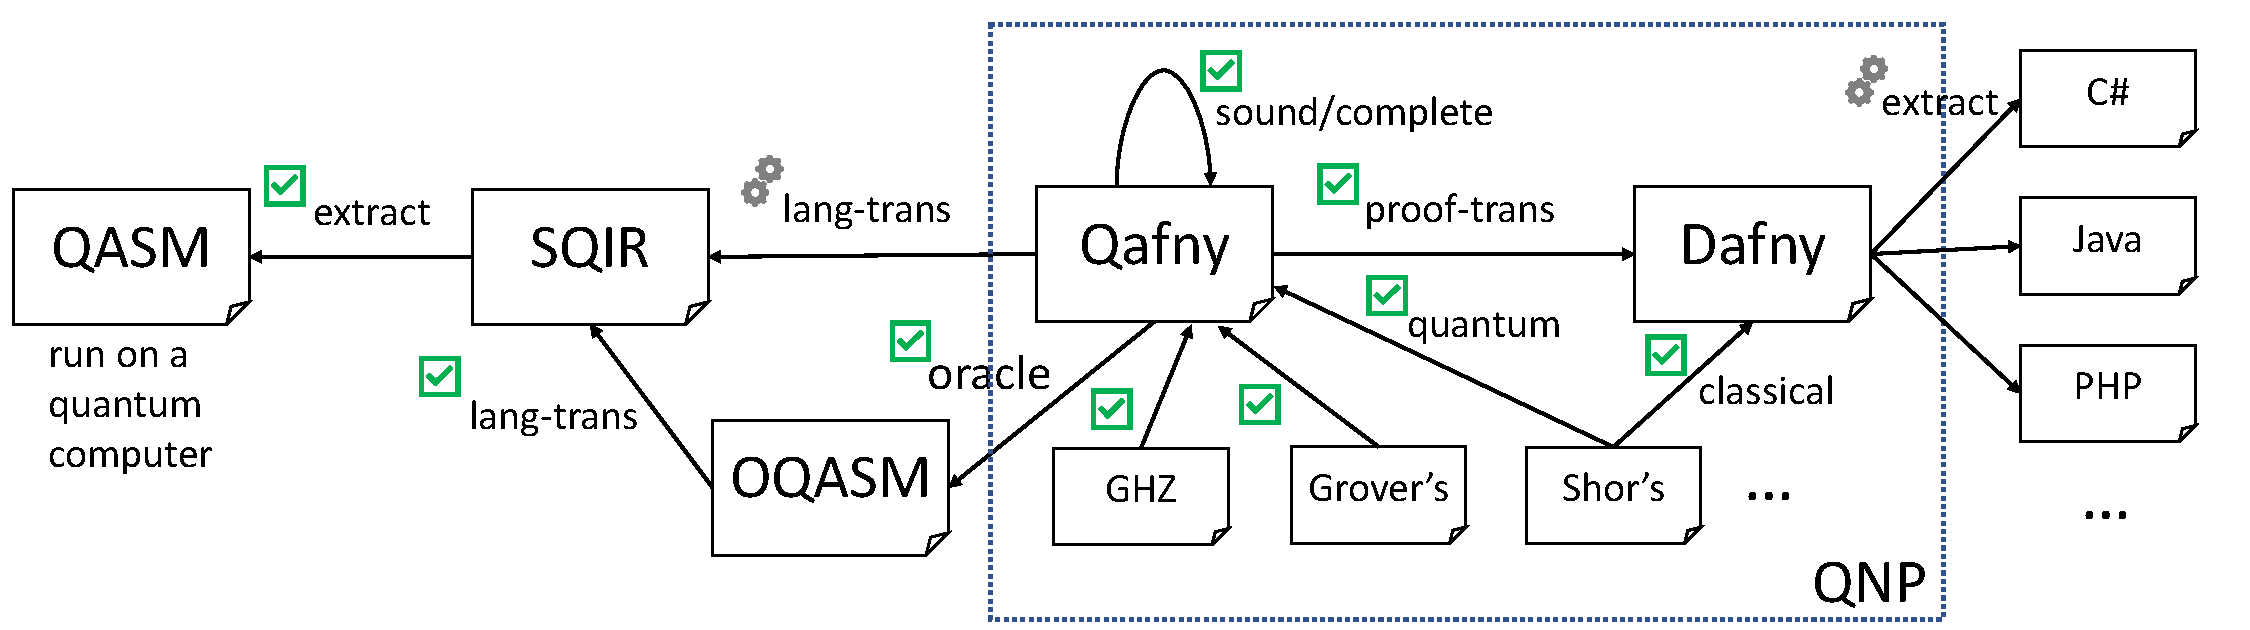
\includegraphics[width=.75\textwidth]{qnp.pdf}
\vspace*{-0.5em}
  \caption{QNP Development Stages and the Key Aspects}
\label{fig:arch}
\end{figure}
\vspace*{-0.5em}

In this paper, we propose \emph{Quantum Natural Proof} (QNP), a framework that help programmers write and verify quantum programs based on the marriage of quantum program semantics and classical automated verification infrastructure. It has several elements, as shown in \Cref{fig:arch}:
1) Using QNP, a quantum program can be specified in a simple, high-level programming
language \qafny, which has standard imperative features and
can express quantum classical hybrid programs with high-level operations,
such as state preparation, oracle, quantum diffusion, quantum conditionals, and for-loops;
2) QNP provides a quantum classical hybird proof system that allows programmers to automatically verify their programs in \qafny.
The quantum portion of the proof system is named the \qafny proof system,
which is specified based on the \qafny quantum language semantics, while the classical part is handled by Dafny \cite{dafnyref};
3) The automated verification in \qafny is compiled to Dafny and utilizes its infrastructure in finishing the task, while the classical component is soley relied on the Dafny proof system, e.g., GHZ and Grover's search algorithms are verified by \qafny, while Shor's algorithm is split into quantum and classical components that are handled by \qafny and Dafny, respectively;
and 4) The \qafny quantum components can be compiled to quantum circuits and run on a quantum computer via the \qafny to SQIR compiler and SQIR to OpenQASM 2.0 \cite{Cross2017} compiler, while the classical components are based on the Dafny infrastructure that can be extracted to several different programming languages, such as C\#, Java and PHP.
%Programmers specify a quantum classical hybrid program specification in QNP. The quantum component verification is relied on the \qafny proof system that translates the quantum part to Dafny and utilizes Dafny's proof infrastructure in finishing the verification, while the classical component is soley relied on the Dafny proof system. For examples, GHZ and Grover's search algorithms have only quantum components and they are verified by \qafny, while Shor's algorithm is split into quantum and classical components, which are verified by \qafny and Dafny, respectively and collaboratively.
%\item The \qafny quantum components can be compiled to quantum circuits and run on a quantum computer via the \qafny to SQIR compiler. 
%We compile a \qafny program to SQIR by partially evaluating its classical components, which can be distinguished by the \qafny type system, and only compile its quantum parts to SQIR,  a circuit language embedded in the Coq proof assistant \cite{PQPC,VOQC}.
%The quantum compilation has two procedures: 1) quantum oracle operations are compiled to SQIR through an intermediate oracle language \oqasm \cite{oracleoopsla}, and 2) the other quantum components are compiled directly to SQIR. SQIR circuits can be optimized and extracted to OpenQASM 2.0 \cite{Cross2017} to run on a real quantum machine. The \qafny classical components are based on the Dafny infrastructure that can be extracted to several different programming languages, such as C\#, Java and PHP. 
% OQASM
% - QFT, Eff. simulatable, virtual qubits
% - Proved-correct comp. to SQIR

\noindent\textbf{\textit{Motivating Examples and Key Design Principles.}}
The key QNP design philosophy leverages the methodology of analogizing quantum operations as classical aggregate operations.
An example that motivates the QNP development is the state preparation in Child's quantum Boolean equation algorithm \cite{ChildsNAND}, as shown in \Cref{fig:intros-example},
where we first prepare a superposition state $\Msum_{j=0}^{2^n}\ket{j}$ \footnote{$2^n$ is excluded from $j$. } by applying $n$ Hadamard operations (see \Cref{sec:background} for quantum background), then apply an oracle operation $f(\ket{\kappa})=(-i)^{\kappa}\ket{\kappa}$.
The oracle operation can be translated as $f(z,\kappa)=((-i)^{\kappa}z,\kappa)$, where we multiply the value $(-i)^{\kappa}$ to the first element in a pair.
If we view the superposition state as an $2^n$ element array, with elements being basis states, the oracle application on the state is exactly a map operation that applies the function $f$ to every array element as in \Cref{fig:intro-example-analog}.
%What we find out is that most quantum operations can be viewed as some aggregate operations and quantum computers essentially provide an efficient way of applying such aggregate operations.
Obviously, quantum algorithms have more complicated structures than a simple array map.
Let's analyze the GHZ example in \Cref{fig:background-circuit-example-proof}. Before entering the for-loop (line 4-6), the input quantum array is split into conceptually two parts, analogized in \Cref{fig:background-circuit-analogy}. 
The two parts have different types. Here, the red part is an array of basis states, while the blue part is an array of qubits.
In each step, we cut one qubit from the blue part and insert it into the white place in the red part by transforming the qubit type.
During this process, the red array structure might vary depending on the inserted qubit state type.
Finally, a quantum conditional is applied on the red array.
Many quantum algorithms have similar structures as the above scenario, such as GHZ \cite{Greenberger1989} and Shor's algorithms. 

QNP is designed to capture the scenario and similar algorithm patterns with two features. First, the language operations in \qafny are designed to be analogized to high level array aggregate operations, so that not only programmers can write programs based on high level operations, but also does the \qafny proof system connect to traditional separation logic; thus, we can then utilize a classical automated proof engine, like Dafny, to automatically verify quantum programs, as our \qafny to Dafny compiler in \Cref{sec:dafny-compilation};
while most quantum proof systems, such as QHL \cite{qhoreusage}, QBricks \cite{qbricks},  QSL/BI \cite{qsepa}, and QSL \cite{quantumseparation}, built proof systems based on quantum computation theories
%The proof system compilation is based on viewing \qafny quantum operations as classical array aggregate operations, i.e., the operations presented in \Cref{fig:intros-example} can be easily verified by Danfy's array operation libraries regardless the exponential state size.
Second, a type system that tracks qubit array bounds and the qubit state type transformation, as the scenario indicates, is designed in QNP. Apparently, tracking bounds in quantum arrays is not as easy as tracking classical array bounds, because qubits from different arrays can be entangled together, i.e., their states are not separable. In QNP, we invented the concept \emph{sessions}, representing groups of qubit array pieces that are possibly entangled with each other. Tracking quantum array bounds is to track the session scopes in our type system that ensures that applications on a session do not interfere with others. 

\noindent\textbf{\textit{Contributions.}}
We identify several QNP achieves as follows, which are partly indicated in \Cref{fig:arch}.
%The second level is the proof system. While most quantum proof systems, such as QHL \cite{qhoreusage}, QBricks \cite{qbricks},  QSL/BI \cite{qsepa}, and QSL \cite{quantumseparation}, built proof systems based on quantum computation theories, QNP tries to connect the \qafny proof system to traditional separation logic; thus, we can then utilize a classical automated proof engine, like Dafny, to automatically verify quantum programs, as our \qafny to Dafny compiler in \Cref{sec:dafny-compilation}.The proof system compilation is based on viewing \qafny quantum operations as classical array aggregate operations, i.e., the operations presented in \Cref{fig:intros-example} can be easily verified by Danfy's array operation libraries regardless the exponential state size.
%QNP is designed to reflect the analogy and has two levels of advantages: the programming language and the automated proof system levels. The QNP programming language, \qafny, permits the quantum operations that can be compiled to quantum circuits.
%In \qafny, we think about program operations as their functionality such as preparing superposition states, applying aggregate oracle operations, quantum conditionals, etc. For example, \Cref{fig:intros-example} is implemented as a state preparation operation, that is compiled to $n$ Hadamard gates, followed by an oracle function $f$. The GHZ \cite{Greenberger1989} implemention in \Cref{fig:background-circuit-example-proof} is a single gate state preparation followed by a for-loop to entangle a list of qubits. 
% by using Hadamard ($\texttt{H}$) and quantum Fourier transform ($\texttt{QFT}$) operations. \Cref{fig:background-circuit-example-proof} Line 2 applies a $\texttt{H}$ operation on $x[0]$, the $0$-th position of the array $x$, but the application can also be applied on the whole array, to prepare superposition of $n$-qubits, as in \Cref{fig:shorqafny}. After the \texttt{H} operator, in the standard implementation of the Greenberger-Horne-Zeilinger (GHZ) circuit \cite{Greenberger1989}, they applies $n-1$ \emph{controlled-not} (\coqe{CNOT}) gates. as shown in \Cref{fig:background-circuit-examplea}. However, in \qafny, we think of \coqe{CNOT} gate's behavior as an application of $n-1$ for-loop steps of quantum conditionals in \Cref{fig:background-circuit-example-proof} line 4-6. In the $j$-th step, the array $x[0..n]$, 
%The second level is the proof system. While most quantum proof systems, such as QHL \cite{qhoreusage}, QBricks \cite{qbricks},  QSL/BI \cite{qsepa}, and QSL \cite{quantumseparation}, built proof systems based on quantum computation theories, QNP tries to connect the \qafny proof system to traditional separation logic; thus, we can then utilize a classical automated proof engine, like Dafny, to automatically verify quantum programs, as our \qafny to Dafny compiler in \Cref{sec:dafny-compilation}.
%The proof system compilation is based on viewing \qafny quantum operations as classical array aggregate operations, i.e., the operations presented in \Cref{fig:intros-example} can be easily verified by Danfy's array operation libraries regardless the exponential state size.
%Indeed, quantum gate applications are linear in the sense that the whole state effect can be viewed as a synthesized effect of applications on individual basis states. For example, applying a $\texttt{X}$ gate on the first qubit in a Bell pair $\frac{1}{\sqrt{2}}(\ket{00} + \ket{11})$ is equal to $\frac{1}{\sqrt{2}}(\texttt{X}\ket{00} + \texttt{X}\ket{11})$, the sum of applying the gate on the second elment of the individual basis states.

\begin{itemize}

\item We define the \qafny semantics as a small-step semantics, and the \qafny proof system based on viewing quantum operations as array aggregate operations. Especially, we define a quantifier free proof rule for quantum conditionals and for-loops whose Boolean guards involve quantum variables. To the best of our knowledge, this is the first inference rule definition for quantum conditionals and for-loops. 

\item We proved in Coq the \qafny type system soundness as well as the proof system soundness and completeness with respect to the \qafny semantics on type-correct programs.

\item We proved in Coq the \qafny to separation logic proof system compilation correctness, as a verification for the \qafny to Dafny compiler. To the best of our knowledge, this is the first work that connects a quantum proof system and classical separation logic proof system.

\item We implemented the \qafny proof system on Dafny, a proof framework based on separation logic, and verified many quantum algorithms (\Cref{fig:circ-evaluation}) with automation. For example, users do not need to specify any teal parts in \Cref{fig:background-circuit-example-proof} and \Cref{fig:shorqafny}, as they are inferred by the \qafny proof system. \Cref{sec:arith-oqasm} shows that program specifications in QNP can be a lot shorter than other quantum proof systems and QNP saves human efforts in verifying quantum programs.

\item We also show in \Cref{sec:arith-oqasm} two case studies that QNP can help programmers to construct verification for new quantum algorithms based on the reuse of existing quantum algorithm proofs. Programmers can also learn about the intuitive behaviors of quantum programs that are previously described as physical procedures. 

\item The circuit compilation from \qafny to OQASM is verified in Coq, while the one from \qafny to SQIR is tested by extracting a \qafny interpreter to Ocaml, and we test program behaviors in the interpreter against the extracted OpenQASM code from SQIR. 
\end{itemize}

\begin{figure}[t]
  \centering
    \captionsetup[subfigure]{justification=centering}
{
\begin{tabular}{l}
\begin{minipage}[t]{.5\textwidth}
\subcaption{State Preparation Circuit}
{\quad
  \small
  \Qcircuit @C=0.5em @R=0.5em {
 \lstick{\ket{0}}  & \qw    & \gate{H} & \qw & \multigate{3}{f(\ket{\kappa})=(-i)^{\kappa}\ket{\kappa}}   & \qw &\qw & \qw \\
   &  \vdots &          &     &                                          &    \rstick{\Msum_{j=0}^{2^n}(-i)^{j}\ket{j}} & &\\
   & \vdots  &          &     &                                          &     &       &  \\
  \lstick{\ket{0}} &  \qw   & \gate{H} & \qw &  \ghost{f(\ket{\kappa})=(-i)^x\ket{\kappa}}         &\qw  &\qw    & \qw
    }
}
\label{fig:intros-example}
\end{minipage}
%
\begin{minipage}[t]{.4\textwidth}
\subcaption{State Preparation Analogy}
{
\small
  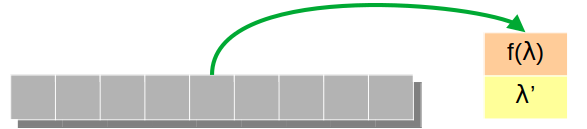
\includegraphics[width=1\textwidth]{oracle}
}
\label{fig:intro-example-analog}
\end{minipage}
\\[-1em]
\begin{tabular}{c c}
\begin{tabular}{l}
\begin{minipage}[t]{.38\textwidth}
\subcaption{GHZ Circuit}
{\qquad
  \small
  \Qcircuit @C=0.5em @R=0.5em {
    \lstick{\ket{0}} & \gate{H} & \ctrl{1} & \qw &\qw & & \dots & \\
    \lstick{\ket{0}} & \qw & \targ & \ctrl{1} & \qw & &  \dots &  \\
    \lstick{\ket{0}} & \qw & \qw   & \targ & \qw & &  \dots &  \\
    & \vdots &   &  &  & & & \\
    & \vdots &  & \dots & & & \ctrl{1} & \qw  \\
    \lstick{\ket{0}} & \qw & \qw & \qw &\qw &\qw & \targ & \qw
    }
}

\label{fig:background-circuit-examplea}
\end{minipage}
\\
\begin{minipage}[t]{.38\textwidth}
\subcaption{GHZ For-loop Analogy}
{
\small
  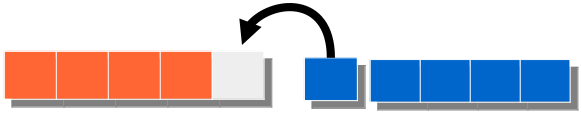
\includegraphics[width=1\textwidth]{ghzforloop}
}
\label{fig:background-circuit-analogy}
\end{minipage}
\end{tabular}
&
\begin{tabular}{l}
\begin{minipage}[t]{.6\textwidth}
\subcaption{\qafny GHZ Program and Proof}
{\small
\[\hspace*{-2em}
\begin{array}{r l}
\textcolor{blue}{1}
&
\textcolor{purple}{
\{x[0..n]\mapsto \ket{\overline{0}}\}
}
\\[0.3em]
\textcolor{blue}{2}
&
\ssassign{x[0]}{}{\ihadh};\\[0.2em]

\textcolor{blue}{3}
&
\textcolor{teal}{
\{x[0..1]\mapsto \frac{1}{\sqrt{2}}(\ket{0}+\ket{1}) * x[1..n]\mapsto \ket{\overline{0}}\}
}
\\[0.3em]

\textcolor{blue}{4}
&
\texttt{for}~{(\texttt{int}~j \in [0,n\,\sminus\,1)~\&\&~x[j])}
\\[0.3em]

\textcolor{blue}{5}
&
\quad
\textcolor{purple}{
\{x[0..\snext{j}]\mapsto \schii{2}{\frac{1}{\sqrt{2}}}{\overline{i}} * x[\snext{j}..n]\mapsto \ket{\overline{0}} * \snext{j} < n\}
}
\\[0.3em]

\textcolor{blue}{6}
&
\quad\;\;
\ssassign{x[\snext{j}]}{}{x[\snext{j}]+1};
\\[0.3em]

\textcolor{blue}{7}
&
\textcolor{teal}{
\{x[0..n]\mapsto \schii{2}{\frac{1}{\sqrt{2}}}{\overline{i}} * x[n..n]\mapsto \ket{\overline{0}}\}
}
\\[0.3em]

\textcolor{blue}{8}
&
\textcolor{purple}{
\{x[0..n]\mapsto \schii{2}{\frac{1}{\sqrt{2}}}{\overline{i}}\}
}
\end{array}
\]
}
\label{fig:background-circuit-example-proof}
\end{minipage}
\end{tabular}
\end{tabular}
\end{tabular}
}
\vspace*{-1em}
\caption{Motivating Examples. $\snext{j}=j\,\splus\,1$. Assume that we have $\kappa\mapsto \schii{2}{}{\overline{i}}$, then $\slen{\kappa}$ is the length of $\kappa$, and $\ket{\overline{i}}$ refers to $m$ number of $i\in[0,1]$ bits, where $m=\slen{\kappa}$. $*$ is the separation conjunction in separation logic. In (d), black parts are \qafny programs, while purple and teal parts are state predicates. }
\label{fig:background-circuit-example}
\end{figure}







%\section{Background}
\label{sec:background}

Here, we provide background information for quantum computing and classical proof systems.

\myparagraph{Quantum States and Alternative State Representations} A quantum state consists of one or more quantum bits (\emph{qubits}). A qubit can be expressed as a two dimensional vector $\begin{psmallmatrix} \alpha \\ \beta \end{psmallmatrix}$ where $\alpha,\beta$ are complex numbers such that $|\alpha|^2 + |\beta|^2 = 1$.  The $\alpha$ and $\beta$ are called \emph{amplitudes}. 
%
We frequently write the qubit vector as $\alpha\ket{0} + \beta\ket{1}$ where $\ket{0} = \begin{psmallmatrix} 1 \\ 0 \end{psmallmatrix}$ and $\ket{1} = \begin{psmallmatrix} 0 \\ 1 \end{psmallmatrix}$ are \emph{computational basis states}. When both $\alpha$ and $\beta$ are non-zero, we can think of the qubit as being ``both 0 and 1 at once,'' a.k.a. a \emph{superposition}. For example, $\frac{1}{\sqrt{2}}(\ket{0} + \ket{1})$ is an equal superposition of $\ket{0}$ and $\ket{1}$. 
We can join multiple qubits together to form a larger quantum state with the \emph{tensor product} ($\otimes$) from linear algebra. For example, the two-qubit state $\ket{0} \otimes \ket{1}$ (also written as $\ket{01}$) corresponds to vector $[~0~1~0~0~]^T$. 
Sometimes a multi-qubit state cannot be expressed as the tensor of individual states; such states are called \emph{entangled}. One example is the state $\frac{1}{\sqrt{2}}(\ket{00} + \ket{11})$, known as a \emph{Bell pair}.

$n$-qubit quantum states are typically represented as $2^n$ dimensional vectors. Alternatively, the states can be represented as different forms. For example, a newly generated qubit typically has a state $\ket{0}$ or $\ket{1}$, which is named \textit{normal typed state} ($\tnort$) in QNP. $n$ Qubits that are in superposition but not entangled, such as $\frac{1}{\sqrt{2}}(\ket{0} + \ket{1})\otimes ... \otimes \frac{1}{\sqrt{2}}(\ket{0} + \ket{1})$, can be expressed as a summation of tensor products as $\shad{2^n}{n}{\alpha(r_j)}$, where $\alpha(r_j)=e^{2\pi i r}$ and $r \in \mathbb{R}$, which is named \textit{Hadamard typed state} ($\thadt$) in QNP.
$\alpha(r_j)$ is named the \emph{local phase} of the state, which are special quantum amplitudes (see below) such that the norm is $1$, i.e., $\slen{\alpha(r_j)}=1$. In the above state, we can view the local phase $1$ as $e^{0}$, and $\frac{1}{\sqrt{2^n}}e^{0}$ is the amplitude for every basis state.

The most general representation is to express quantum states as a path-sum formula as: $\sch{m}{z_j}{c_j}$, where $z_j\in \mathbb{C}$ is an amplitude, $c_j$ is an $n$-length bitstring named \emph{basis}, and $m \le 2^n$. The path-sum formula is same as ${z_0}\ket{c_0}+...+{z_{m-1}}\ket{c_{m-1}}$, such that each $j$-th element ${z_j}\ket{c_j}$ represents a \emph{basis state} in the superposition state. 
This is named \textit{entanglement typed state} ($\tcht$) in QNP.
For example, the bell pair can be represented as $\sch{2}{\frac{1}{\sqrt{2}}}{c_j}$ with $c_0=00$ and $c_1=11$.
Notice that the amplitudes satisfy the relation $\sum_{0}^{m}\slen{z_j}^2 = 1$. However, in some intermediate program evaluation in QNP, we loose the restriction to be $\sum_{0}^{m}\slen{z_j}^2 \le 1$, because a state $\sch{m}{z_j}{c_j}$ can be split into two parts as $\sch{m}{z_j}{c_j}=\schii{m_1}{z_i}{c_i}+\schk{m_2}{z_k}{c_k}$, and we might only want to reason about a portion of the state $\schii{m_1}{z_i}{c_i}$ locally, so that $\sum_{0}^{m_1}\slen{z_i}^2 < 1$. 

In QNP, each quantum state is associated with a \emph{session}, referring to a cluster of quantum array pieces possibly entangled with each other. We can view a session as a virtual quantum array that manages quantum physical qubit arrays living in different locations but are locally connected through entanglement. See \Cref{sec:quantum-state}.
As a shortcut of basis state representations, we might write $\ket{c_1}\otimes \ket{c_2}=\ket{c_1}\ket{c_2}=\ket{c_1.c_2}$ where $c_1.c_2$ is the bitstring concatenation and $c_1$ and $c_2$ are bitstrings of some sizes that relate to session lengths.
\ignore{
\myparagraph{Sessions}
If we analogize a quantum state $\sch{m}{z_j}{c_j}$ as an $m$-length array and each basis state $z_j\ket{c_j}$ as the $j$-th element in the array. \Cref{fig:background-circuit-example-proof} line 1, we have a singleton array $x[0..n]$, each element of which is $n$-length.
In QNP, we named the name structure referring to an array representing a quantum state as a \emph{session}. Here $x[0..n]$ is a session indicating that the location of the array is in a region named $x$, and the range is from $0$ to $n$, which means that the length of each element is $n$. After the application of $\ssassign{x[0]}{}{\ihadh}$, we split the session into two parts: $x[0..1]$ and $x[1..n]$ having a $\thadt$ type ($\frac{1}{\sqrt{2}}(\ket{0}+\ket{1})$) and $\tnort$ ($\ket{\overline{0}}$) type states, respectively.
Here, the singleton element in $x[1..n]$ is now $n-1$ length.
State $\frac{1}{\sqrt{2}}(\ket{0}+\ket{1})$ can also be viewed as $\sch{2}{\frac{1}{\sqrt{2}}}{\overline{i}}$ with $i\in[0,1]$.
Here, $\overline{i}$ is a singleton bitstring. 
In each step of the loop in line 4-6, we cut off the $j$-th bit in the singleton element array, so the array session becomes $x[\snext{j}..n]$, then we put the bit in the original $x[0..1]$ session which is now structured as $x[0..j]$.
The state becomes $\sch{2}{\frac{1}{\sqrt{2}}}{\overline{i}}\ket{0}$. Notice that the quantum conditional in each loop step applies on the $j$-th and $(\snext{j})$-th bits of the two basis states ($\overline{0}$ and $\overline{1}$). When $i=0$, we do nothing; if $i=1$, we flip the bit, which means that we turn the state to be $\sch{2}{\frac{1}{\sqrt{2}}}{\overline{i}}$, with the $\overline{i}$ length increases by one and it is the same as the length the session $x[0..\snext{j}]$. In the end, we can remove the $x[n..n]\mapsto \ket{\overline{0}}$ in the final state, because session $x[n..n]$ means that each element in the state array is $0$, so we claim such session as empty. 
}

\myparagraph{Quantum Computations and Conditionals} High-level quantum programming languages are usually designed to follow the \emph{QRAM model}~\cite{Knill1996}, where quantum computers are used as co-processors to classical computers. The classical computer generates descriptions of circuits to send to the quantum computer and then processes the measurement results.
Computation on a quantum state consists of a series of \emph{quantum operations}, each of which acts on a subset of qubits in the quantum state. In the standard presentation, quantum computations are expressed as \emph{circuits}, as shown in \Cref{fig:background-circuit-examplea}, which constructs a circuit that prepares the Greenberger-Horne-Zeilinger (GHZ) state \cite{Greenberger1989}, which is an $n$-qubit entangled quantum state of the form: $\ket{\text{GHZ}^n} = \frac{1}{\sqrt{2}}(\ket{0}^{\otimes n}+\ket{1}^{\otimes n})$.

In these circuits, each horizontal wire represents a qubit and boxes on these wires indicate quantum operations, or \emph{gates}. The circuit in \Cref{fig:background-circuit-examplea} uses $n$ qubits and applies $n$ gates: a \emph{Hadamard} (\coqe{H}) gate and $n-1$ \emph{controlled-not} (\coqe{CNOT}) gates.
Applying a gate to a state \emph{evolves} the state. 
The \qafny implementation in \Cref{fig:background-circuit-example-proof} shows the evolving. In the $j$-th loop step, the quantum state of array $x[0..j]$ is $\frac{1}{\sqrt{2}}(\ket{\overline{0}}+\ket{\overline{1}})$ \footnote{$\ket{\overline{0}}$ and $\ket{\overline{1}}$ have the same length as $x[0..j]$}, and a qubit $\ket{0}$ is added to the state and transforms the state to $\frac{1}{\sqrt{2}}(\ket{\overline{0}}\ket{0}+\ket{\overline{1}}\ket{0})$, which adds a bit $0$ to the end of every basis state. Then, the quantum conditional 
($\sifq{x[j]}{\ssassign{x[\snext{j}]}{}{x[\snext{j}]+1}}$) turns $\ket{0}$ in the second basis state to $\ket{1}$ as $\frac{1}{\sqrt{2}}(\ket{\overline{0}}\ket{0}+\ket{\overline{1}}\ket{1})$, because the quantum conditional checks the $j$-th qubit in every basis state, if it is $1$, then the conditional body is applied; otherwise, it does nothing.

\myparagraph{Measurement} A special, non-unitary \emph{measurement} operation is used to extract classical information from a quantum state, typically when a computation completes. Measurement collapses the state to one of the basis states with a probability related to the state's amplitudes. For example, measuring $\frac{1}{\sqrt{2}}(\ket{0} + \ket{1})$ will collapse the state to $\ket{0}$ with probability $\frac{1}{2}$ and likewise for $\ket{1}$, returning classical values 0 or 1, respectively.

\myparagraph{Quantum Oracles} Quantum algorithms manipulate input information encoded in ``oracles,'' which are callable black box circuits. For example, Grover's algorithm for unstructured quantum search \cite{grover1996,grover1997} is a general approach for searching a quantum ``database,'' which is encoded in an oracle for a function $f : \{0, 1\}^n \to \{0, 1\}$. Grover's finds an element $x \in \{0, 1\}^n$ such that $f(x) = 1$ using $O(2^{n/2})$ queries, a quadratic speedup over the best possible classical algorithm, which requires $\Omega(2^n)$ queries. Oracles are typically viewed as quantum reversible implementations of classical operations, especially arithmetic operations. OQASM \cite{oracleoopsla} is a language that permits the effective testing of quantum oracles.

\myparagraph{Dafny and Natural Proof} Dafny \cite{10.1007/978-3-642-17511-4_20} is a language that is designed to make it easy to write correct code. It permits imperative programming with logical specifications which can be automatically verified through the Dafny proof system, a separation logic based system. The natural proof methodology was first proposed by Madhusudan \textsf{et al.} \cite{nat-proof,10.1145/2103621.2103673}, which exploits a fixed set of proof tactics, keeping the expressiveness of powerful logics, retaining the
automated nature of proving validity, but giving up on completeness, e.g., the \qafny to Dafny compilation is only sound but not complete. 
The \qafny implementation of the natural proof methodology identifies a subclass of proofs $\mathpzc{N}$ such that
(1) a large class of valid verification specifications of near term classical quantum hybrid programs have a proof in $\mathpzc{N}$, 
and (2) searching for a proof in $\mathpzc{N}$ is efficiently decidable. 
In the original natural proof, the subclass identification is based on mapping heap data-structures, such as trees and link lists, to logical invariant properties. In QNP, the identification is through the \qafny type system in classifying quantum sessions and state types so that quantum operation applications on a specific session can be compiled to classical aggregate operations that have rich proof infrastructures in Dafny. 











%\input{overview}
\section{Qafny: A High-level Quantum Language Admitted a Proof System}
\label{sec:qafny}

Here, we first introduce \qafny state equational properties and type system. Then, we discuss its semantics and proof system.

\subsection{State Equivalence, Type, and Sequence Rules}\label{sec:state}

\begin{figure}
{\footnotesize
{\hspace*{-6em}
\begin{minipage}[t]{0.35\textwidth}
\begin{center}
 \[
  \begin{array}{l@{~}cl}
  \tau & \sqsubseteq & \tau \\
  \tnort &\sqsubseteq& \tcht\\
  \thadt &\sqsubseteq& \tcht
    \end{array}
  \]
\end{center}
\subcaption{Subtyping}
  \label{fig:qafny-subtype}
\end{minipage}
\qquad
\begin{minipage}[t]{0.5\textwidth}
\begin{center}
   \[
   \begin{array}{l@{~}cl}
   q & \equiv_{\slen{q}} & q \\
  \ket{c} &\equiv_n& \sch{1}{ }{c}\\
  \shad{2^n}{n}{\alpha(r_j)} &\equiv_n& \sch{2^n}{\frac{\alpha(\sum_{k=0}^{n} r_k \cdot \tos{j}[k])}{\sqrt{2^n}}}{j}
    \end{array}
 \]
\end{center}
\subcaption{Quantum Value Equivalence}
  \label{fig:qafny-sequiv}
\end{minipage}
\hfill{}
\begin{minipage}[t]{0.8\textwidth}
\begin{center}
 \[
  \begin{array}{l @{~} c @{~} l l@{~}c @{~} l l @{~}c @{~} l l @ {~} c @{~} l}
\lambda &\equiv & \lambda
&
\qquad
x[n,n] & \equiv & \bot
&
\qquad
\bot \uplus \lambda & \equiv & \lambda
&
\qquad
x[n,m]\uplus\lambda & \equiv & x[n,j]\uplus x[j,m] \uplus\lambda
\\
&&&&&&&&&&&
\texttt{where}\;\;n \le j < m

    \end{array}
  \]
\end{center}
\subcaption{Session Equivalence}
  \label{fig:qafny-ses-equal}
\end{minipage}
\hfill{}
\hspace*{-5em}
\begin{minipage}[t]{0.475\textwidth}
\begin{center}
 \[
  \begin{array}{l@{~}c@{~}l}
    \sigma & \preceq & \sigma \\[0.2em]
  \{\bot:\tau\} \cup \sigma &\preceq& \sigma\\[0.2em]
   \{\lambda:\tau\} \cup \sigma &\preceq& \{\lambda:\tau'\} \cup \sigma\\
&&\texttt{where}\;\;\tau\sqsubseteq_{\slen{\lambda}}\tau' \\[0.2em]
  \{\lambda_1\uplus l_1 \uplus l_2 \uplus \lambda_2 :\tau\} \cup \sigma &\preceq& \{\lambda_1\uplus l_2 \uplus l_1 \uplus \lambda_2 : \tau\} \cup \sigma\\[0.2em]
  \{\lambda_1 :\tau\} \cup \{\lambda_2 :\tau\} \cup \sigma &\preceq& \{\lambda_1 \uplus \lambda_2 :\tau\} \cup \sigma \\[0.2em]
  \{\lambda_1 \uplus \lambda_2 :\tau\} \cup \sigma &\preceq& \{\lambda_1 :\tau\} \cup \{\lambda_2 :\tau\} \cup \sigma
\\
&&\texttt{where}\;\;\tau\neq\tcht
    \end{array}
  \]
\end{center}
\subcaption{Environment Equivalence}
  \label{fig:env-equiv}
\end{minipage}
\begin{minipage}[t]{0.475\textwidth}
\begin{center}
   \[
   \begin{array}{l@{~}c@{~}l}
    \varphi & \equiv & \varphi \\[0.2em]
  \{\bot:q\} \cup \varphi &\equiv& \varphi\\[0.2em]
   \{\lambda:q\} \cup \varphi &\equiv& \{\lambda:q'\} \cup \varphi\\
   &&\texttt{where}\;\;q\equiv_{\slen{\lambda}}q' 
   \\[0.2em]
  \{\lambda_1\uplus l_1 \uplus l_2 \uplus \lambda_2 :q\} \cup \varphi &\equiv& \{\lambda_1\uplus l_2 \uplus l_1 \uplus \lambda_2 : \texttt{mut}(q,\slen{\lambda_1})\} \cup \varphi\\[0.2em]
  \{\lambda_1 :q_1\} \cup \{\lambda_2 :q_2\} \cup \varphi &\equiv& \{\lambda_1 \uplus \lambda_2 :\texttt{mer}(q_1,q_2)\} \cup \varphi 
   \\[0.2em]
  \{\lambda_1 \uplus \lambda_2 :\varphi\} \cup \sigma &\equiv& \{\lambda_1 :\varphi_1\} \cup \{\lambda_2 :\varphi_2\} \cup \sigma
\\
&&\texttt{where}\;\;\texttt{spt}(\tau,\slen{\lambda_1})=(\varphi_1,\varphi_2)
    \end{array}
 \]
\end{center}
\subcaption{State Equivalence}
  \label{fig:qafny-stateequiv}
\end{minipage}
{\footnotesize
\[
\begin{array}{l}
\texttt{pmut}((c_1.i_1.i_2.c_2),n)=(c_1.i_2.i_1.c_2) \;\;\texttt{when}\;\slen{c_1}=n
\\[0.2em]
\texttt{mut}(\ket{c},n)=\ket{\texttt{pmut}(c,n)}
\\[0.2em]
\texttt{mut}(\frac{1}{\sqrt{2^m}}(q_1 \bigotimes (\ket{0}+\alpha(r_n)\ket{1}) \bigotimes (\ket{0}+\alpha(r_{n+1})\ket{1}) \bigotimes q_2),n)
\\
\qquad\qquad
=\frac{1}{\sqrt{2^m}}(q_1 \bigotimes (\ket{0}+\alpha(r_{n+1})\ket{1}) \bigotimes (\ket{0}+\alpha(r_n)\ket{1}) \bigotimes q_2)
\quad\texttt{when\;}\slen{q_1}=n
\\[0.2em]
\texttt{mut}(\sch{m}{z_j}{c_j},n)=\sch{m}{z_j}{\texttt{pmut}(c_j,n)}
\\[0.2em]
\texttt{mer}(\ket{c_1},\ket{c_2})=\ket{c_1.c_2}
\\[0.2em]
\texttt{mer}(\shad{2^n}{n}{\alpha(r_j)},\shad{2^m}{m}{\alpha(r_j)})=\shad{2^{n+m}}{n+m}{\alpha(r_j)}
\\[0.2em]
\texttt{mer}(\sch{n}{z_j}{c_j},\schk{m}{z_k}{c_k})=\schi{n*m}{z_j\cdot z_k}{c_j.c_k}
\\[0.2em]
\texttt{spt}(\ket{c_1.c_2},n)=(\ket{c_1},\ket{c_2}) \;\;\texttt{when}\;\slen{c_1}=n
\\[0.2em]
\texttt{spt}(q_1\bigotimes q_2,n)=(q_1,q_2) \;\;\texttt{when}\;\slen{q_1}=n
\end{array}
\]
}
  \caption{\qafny type/state relations. $\{\tos{j}|j\in[0,2^n)\}(2^n)$ defines a set $\{\tos{j}|j\in[0,2^n)\}$ with the emphasis that it has $2^n$ elements. $\{0,1\}$ is a set of two single element bitstrings $0$ and $1$. $\cdot$ is the multiplication operation, $\tos{j}$ turns a number $j$ to a bitstring, $\tos{j}[k]$ takes the $k$-th element in the bitstring $\tos{j}$, and $\ket{j}$ is an abbreviation of $\ket{\tos{j}}$. We use set union ($\cup$) to describe the state concatenation with the empty set operation $\emptyset$. $i$ is a single bit either $0$ or $1$. The $.$ operation is bitstring concatenation. Term $\Msum^{n*m}P$ is a summation formula that omits the indexing details.
Term $(\frac{1}{\sqrt{2^{n}}}\Motimes_{j=0}^{n}q_j) \bigotimes(\frac{1}{\sqrt{2^{m}}}\Motimes_{j=0}^{m}q_j)$ is equivalent to $\frac{1}{\sqrt{2^{n+m}}}\Motimes_{j=0}^{n+m}q_j$.}
  \label{fig:qafny-eq}
}
}
\end{figure}

As we suggested in \Cref{sec:shors}, quantum states have certain level of permutation symmetries. Essentially, quantum computation is implemented as circuits. In \Cref{fig:background-circuit-example}, if the first and second circuit lines and qubits are permuted, it is intuitive that the two circuit results are equivalence up to the permutation. Additionally, as indicated in \Cref{sec:shors}, we need quantum sessions to be split and regrouped sometimes. All these properties are formulated in \qafny as equational properties in \Cref{fig:qafny-eq} that rely on session rewrites, which can then be used as builtin libraries in the proof system. As one can imagine, the equational properties might bring nondeterminism in the \qafny implementation, such that the automated system does not know which equations to apply in a step. In dealing with the nondeterminism, we design a type system for \qafny to track the uses, split, and join of sessions, as well as the three state types in every transition step, so that the system knows exactly how to apply an equation.

\myparagraph{State Equivalence}
\Cref{fig:qafny-eq} shows the equivalence relations on types and states.
\Cref{fig:qafny-subtype} shows the subtyping relation such that $\tnort$ and $\thadt$ subtype to $\tcht$.
Correspondingly, the subtype of $\tnort$ to $\tcht$ represents the first line equation in \Cref{fig:qafny-sequiv}, where a $\tnort$ state is converted to a $\tcht$ form. Similarly, a $\thadt$ state can also be converted to a $\tcht$ state in the second line.
Additionally, \Cref{fig:qafny-ses-equal} defines the equivalence relations for the session concatenation operation $\uplus$: it is associative, identitive with the identity empty session element $\bot$.
We also view a range $x[n,n]$ to be empty ($\bot$), and a range $x[n,m]$ can be split into a two ranges in the session as $x[n,j] \uplus x[j,m]$. 

The main result to define state equivalence is to capture the permutation symmetry, split, and join of sessions introduced in \Cref{sec:shors}. The first rule describes the case for empty session, while the second rule in \Cref{fig:qafny-stateequiv} connects the quantum value equivalence to the state equivalence.
The third rule describes the qubit permutation equivalence by the \texttt{mut} function.
The fourth rule describes the join of two sessions in a state.
For the two sessions are of the type $\tnort$ and $\thadt$, a join means an array concatenation.
If the two sessions have $\tcht$ types, a join means a Cartesian product of the two basis states.
The final rule is to split a session, where we only allows the split of a $\tnort$ and $\thadt$ type state and their splits are simply array splits. Splitting a $\tcht$ type state is equivalent to qubit disentanglement, which is a hard problem and we need to upgrade the type system to permit certain types of such disentanglement. In \Cref{sec:newtype}, we upgrade the \qafny type system to a dependent type system to track the disentanglement of $\tcht$ type state.


\begin{figure}[t]
{
{\Small
  \begin{mathpar}
    \inferrule[TPar]{\sigma \preceq \sigma' \\ \Omega;\sigma' \vdash_g s \triangleright \sigma''}{\Omega;\sigma \vdash_g s \triangleright \sigma'' }

    \inferrule[TEXP]{\Omega[x\mapsto \cmode];\sigma\vdash_g s[n/x] \triangleright \sigma'}{\Omega;\sigma \vdash_g \sexp{x}{n}{s} \triangleright \sigma' }

    \inferrule[TMEA]{ \Omega(y)=\qmode{j} \\ \sigma(y) = \{y[0..j]\uplus\lambda\mapsto \tau \}
     \\\\ \Omega[x\mapsto \mmode];\sigma[\lambda \mapsto \tcht]\vdash_{\cmode} s \triangleright  \sigma'}{\Omega;\sigma \vdash_{\cmode} \sexp{x}{\smea{y}}{s} \triangleright \sigma' }

    \inferrule[TA-CH]{ FV(\Omega,\mu)=\lambda\\ \sigma(\lambda\uplus\lambda') = \tcht}{\Omega;\sigma \vdash_g \ssassign{\lambda}{}{\mu} \triangleright \{\lambda\uplus\lambda':\tcht\} }

    \inferrule[TDIS]{ FV(\Omega,l)=\lambda\\ \sigma(\lambda\uplus\lambda') = \tcht}{\Omega,\sigma \vdash_g \ssassign{\lambda}{}{\sdis} \triangleright \{l\uplus\lambda':\tcht\} }

    \inferrule[TSEQ]{\Omega;\sigma\vdash_g s_1 \triangleright\sigma_1
 \\\\\Omega;\sigma[\uparrow \sigma_1]\vdash_g s_2 \triangleright\sigma_2}{\Omega;\sigma \vdash_g \sseq{s_1}{s_2}\triangleright \;\sigma_2\cup\sigma_1|_{\not\in\dom{\sigma_2}} }

\inferrule[TIF]{ 
FV(\Omega,b)=\lambda\\
\lambda\cap FV(\Omega,s) =\emptyset 
\\\\
     \Omega;\sigma[\lambda \mapsto \tcht] \vdash_{\mmode} s \triangleright \{\lambda':\tcht\}} 
{\Omega;\sigma[\lambda \uplus \lambda' \mapsto \tcht] \vdash_g \sifq{b}{s} \triangleright \{\lambda\uplus \lambda':\tcht\} }


    \inferrule[TLOOP]{ \forall j\in[n_1,n_2)\;.\;\Omega;\sigma[\uparrow \sigma'[j/x]]\vdash_g \sifq{b}{s} \triangleright \sigma'[\texttt{S}\;j/x] }
                  {\Omega;\sigma \vdash_g \sqwhile{x}{n_1}{n_2}{b}{s} \triangleright \sigma'[n_2/x]}
  \end{mathpar}
}
{\footnotesize
\[
\sigma[\uparrow \sigma'] = \sigma[\forall \lambda:\tau \in \sigma'\;.\;\tau/\lambda]
\qquad
\sigma|_{\not\in\dom{\sigma'}}=\{\lambda:\tau|\lambda \not\in \dom{\sigma'}\}
\]
}
}
  \caption{\qafny type system. $\sigma(y)=\{\lambda\mapsto \tau\}$ produces the map entry $\lambda\mapsto \tau$ and the range $y[0..\slen{y}]$ is in $\lambda$. $\sigma(\lambda)=\tau$ is an abbreviation of $\sigma(\lambda)=\{\lambda\mapsto \tau\}$. $FV(\Omega, -)$ produces a session by union all qubits appearing in $-$ with the qubit group info in $\Omega$; see \Cref{sec:session-gen}.}
  \label{fig:exp-sessiontype}
\end{figure}

\myparagraph{Type Checking: A Quantum Session Type System}
In \qafny, typing is with respect to a \emph{kind environment} $\Omega$ and a \emph{finite type environment} $\sigma$,
which map \qafny variables to kinds and map sessions to types, respectively.
The typing judgment is written as $\Omega; \sigma\vdash_{g} s \triangleright \sigma'$,
which states that statements $s$ is well-typed under the context mode $g$ and environments $\Omega$ and $\sigma$,
the sessions representing $s$ is exactly the domain of $\sigma'$ as $\dom{\sigma'}$,
and $s$ transforms types for the sessions in $\sigma$ to types in $\sigma'$.
$\Omega$ describes the kinds for all program variables.
$\Omega$ is populated through \texttt{let} expressions that introduce variables,
and the \qafny type system enforces variable scope; such enforcement is neglected in \Cref{fig:exp-sessiontype} for simplicity.
We also assume that variables introduced in \texttt{let} expressions are all distinct through proper alpha conversions.
$\sigma$ and $\sigma'$ describe types for sessions referring to possibly entangled quantum clusters pointed to by quantum variables in $s$. 
$\sigma$ and $\sigma'$ are both finite and the domain of them contain sessions that do not overlap with each other; $\dom{\sigma}$ is large enough to describe all sessions pointed to by quantum variables in $s$,
while $\dom{\sigma'}$ should be the exact sessions containing quantum variables in $s$.
Selected type rules are given in \Cref{fig:exp-sessiontype}; the rules not mentioned are similar and listed in \Cref{sec:qafny-app}.

The type system enforces five invariants.  First, well-formed and context restrictions for quantum programs.
Well-formedness means that qubits mentioned in the Boolean guard of a quantum conditional cannot be accessed in the conditional body,
while context restriction refers to the fact that the quantum conditional body cannot create (\texttt{init}) and measure (\texttt{measure}) qubits. 
For example the $FV$ checks in rule \textsc{TIF} enforces that the session for the Boolean and the conditional body does not overlap.
Coincidentally, we utilize the modes ($g$, either $\cmode$ or $\mmode$) as context modes for the type system. 
Context mode $\cmode$ permits most \qafny operations. Once a type rule turns a mode to $\mmode$, such as in the conditional body in rule \textsc{TIF}, we disallow \texttt{init} and \texttt{measure} operations. For example, rules \textsc{TMEA} is valid only if the input context mode is $\cmode$.

Second, the type system tracks the basis state of every qubit in sessions. In rule \textsc{TA-CH}, we find that the oracle $\mu$ is applied on $\lambda$ belonging to a session $\lambda \uplus \lambda'$. The $\mu$ application preserves the session in $\tcht$ provided that the input type is turned to $\tcht$ type through rule $\textsc{TPar}$.
Third, the type system enforces equational properties of 
quantum qubit sessions through a partial order relation over type environments, including subtyping, qubit position permutation, merge and split quantum sessions through rule $\textsc{TPar}$.
Essentially, we can view two qubit arrays be equivalent if there is a bijective permutation on the qubit positions of the two.
To analyze a quantum application on a qubit array, if the array is arranged in a certain way, the semantic definition will be a lot more trivial than other arrangements. For example, in applying a quantum oracle to a session (rule \textsc{TMEA}), we fix the qubits that permits the $\mu$ operation to always live in the front part ($\lambda$ in $\lambda\uplus\lambda'$).
This is achieved by a consecutive application of the mutation rule ($\texttt{mut}$) in the partial order ($\preceq$) in \Cref{fig:env-equiv}, which casts the left type environment to the format on the right through rule \textsc{TPar}.

Fourth, the type system enforces that the $\cmode$ classical variables can be evaluated to values in the compilation time. \footnote{We consider all computation that only needs classical computer is done in the compilation time.}, while tracks $\mmode$ variables which represent the measurement results of quantum sessions. Rule \textsc{TEXP} enforces that a classical variable $x$ is replaced with its assignment value $n$ in $s$. The substitution statement $s[n/x]$ also evaluates classical expressions in $s$, which is described in \Cref{sec:qafny-app}.
Finally, the type system extracts the result type environment of a for-loop as $\sigma'[n_2/x]$ based on the extraction of a type environment invariant on the $i$-th loop step of executing a conditional $\sifq{b}{s}$ in rule \textsc{TLOOP}, regardless if the conditional is classical or quantum. 

\begin{figure*}[t]
{\small
\begin{tabular}{l}   
{\noindent\textcolor{blue}{\text{Predicate modeling:}}}\\

  \begin{mathpar}
    \inferrule[]{\Omega;\sigma\vdash \lambda \\  \models \varphi(\lambda) \mapsto q }{\Omega;\sigma,\varphi\models \lambda \mapsto q }

    \inferrule[]{ q\equiv_{\slen{q}} q' }{\models q \mapsto q' }

    \inferrule[]{ \sch{m}{z_j}{c_j} \subseteq \sch{m}{z'_j}{c'_j} \\ 
             \sch{m}{z'_j}{c'_j} \subseteq \sch{m}{z_j}{c_j} }{\models \sch{m}{z_j}{c_j} \mapsto \sch{m}{z'_j}{c'_j} }

    \inferrule[]{\sigma \bot \sigma' \\ \varphi \bot \varphi' 
      \\ \Omega;\sigma, \varphi \models P \\ \Omega;\sigma',\varphi' \models Q}
        {\Omega;\sigma \cup \sigma',\varphi \cup \varphi'\models P * Q }

    
  \end{mathpar}

\\[1em]
{\noindent\textcolor{blue}{\text{Sequence Semantic and Proof Rules:}}}\\[0.5em]


  \begin{mathpar}
    \inferrule[SSeq-1]{(\varphi,s_1) \longrightarrow (\varphi',s'_1)}{(\varphi,\sseq{s_1}{s_2})\longrightarrow (\varphi',\sseq{s'_1}{s_2}) }

    \inferrule[SSeq-2]{}{(\varphi,\sseq{\{\}}{s_2})\longrightarrow (\varphi,s_2) }

    \inferrule[PSeq]{
          \Omega;\sigma\vdash_g s_1 \triangleright \sigma' \\\\
       \fivepule{\Omega}{\sigma}{g}{P}{s_1}{R} \\ 
           \fivepule{\Omega}{\sigma[\uparrow \sigma']}{g}{R}{s_2}{Q}}
                {\fivepule{\Omega}{\sigma}{g}{P}{\sseq{s_1}{s_2}}{Q}}

  \end{mathpar}

\\[1em]
{\noindent\textcolor{blue}{\text{Pre-condition strengthening and Post-condition weakening Proof Rules:}}}\\[0.5em]

  \begin{mathpar}
    \inferrule[PConL]{
       (\Omega,\sigma,P) \Rightarrow (\Omega,\sigma',P') \\ \fivepule{\Omega}{\sigma'}{g}{P'}{s}{Q}}
                {\fivepule{\Omega}{\sigma}{g}{P}{s}{Q}}

    \inferrule[PConR]{\Omega,\sigma\vdash_g s_1 \triangleright \sigma'\\\\
          \fivepule{\Omega}{\sigma'}{g}{P}{s}{Q'} \\(\Omega,\sigma'',Q') \nRightarrow (\Omega,\sigma[\uparrow \sigma'],Q) }
                {\fivepule{\Omega}{\sigma}{g}{P}{s}{Q}}
  \end{mathpar}
\end{tabular}
}
{\footnotesize
\[
\begin{array}{l}
\\
(\Omega,\sigma,P) \Rightarrow (\Omega,\sigma',P') \triangleq \Omega,\sigma\vdash P \wedge \Omega,\sigma' \vdash P' \wedge \sigma \preceq \sigma' \wedge P \Rightarrow P'
\\[0.2em]
(\Omega,\sigma,Q) \nRightarrow (\Omega,\sigma',Q') \triangleq \Omega,\sigma\vdash Q \wedge \Omega,\sigma' \vdash Q' \wedge \sigma' \preceq \sigma \wedge Q \Rightarrow Q'
\ignore{
\\[0.2em]
\varphi \equiv \varphi' \wedge \varphi \models P \wedge \varphi' \models P' \Rightarrow (P \Leftrightarrow P') 
}
\end{array}
\]
}
\caption{Sequence and Consequence Rules}
\label{fig:exp-proofsystem-1}
\end{figure*}

\myparagraph{Taste of Semantic and Proof Rules: Sequence and Consequence}
We define the small step operational semantics of an \qafny program as a relation $(\Phi,s) \longrightarrow (\Phi',s')$, where $\Phi$ and $\Phi'$ are the pre- and post- states.

partial function
$\llbracket\rrbracket$ from
an instruction $\instr$ and input state $\varphi$ to an output state
$\varphi'$, written 
$\llbracket \instr \rrbracket\varphi=\varphi'$, shown in \Cref{fig:deno-sem}.


\begin{figure*}[t]
{\small

\begin{minipage}[t]{0.4\textwidth}
\subcaption{Application Analogy}
  \vspace{1cm}
  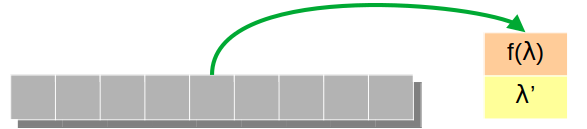
\includegraphics[width=\textwidth]{oracle}
  \label{fig:qafny-oracle-analog}
\end{minipage}
\hfill
\begin{minipage}[t]{0.5\textwidth}
\subcaption{App Function Modeling}
  \begin{mathpar}

    \inferrule[]{\forall j.\;\slen{c_{j1}}=n \\ \Omega;\sigma;\varphi\models \sch{m}{z_j}{\denote{\mu}(c_{j1}).c_{j2}\,\beta_j} \mapsto q}
          {\Omega;\sigma;\varphi\models \eth \;n.\denote{\mu}(\sch{m}{z_j}{c_{j1}.c_{j2}\,\beta_j}) 
              \mapsto q }
  \end{mathpar}
  \label{fig:qafny-mu-model}
\end{minipage}

\begin{minipage}[t]{\textwidth}
\subcaption{Semantic/Proof Rules}
  \begin{mathpar}
    \inferrule[SA-CH]{ \varphi(\lambda)=\{\lambda\uplus\lambda'\mapsto \sch{m}{z_j}{c_{j1}.c_{j2}\,\beta_j}\} \\\\ 
     \forall j.\; \slen{c_{j1}}=\slen{\lambda} \wedge \llbracket \mu \rrbracket c_{j1} = z'_j\ket{c'_{j1}} }{ (\varphi,\ssassign{\lambda}{}{\mu}) \longrightarrow (\varphi[\lambda\uplus\lambda'\mapsto \sch{m}{z'_j\cdot z_j}{c'_{j1}.c_{j2}\,\beta_j}],\{\}) }

    \inferrule[PA-CH]{\sigma(\lambda)=\{\lambda \uplus \lambda' \mapsto \tcht\}}
                {\fivepule{\Omega}{\sigma}{g}{P[\eth \;\lambda.\denote{\mu}(\lambda \uplus \lambda') / \lambda \uplus \lambda']}{\ssassign{\lambda}{}{\mu}}{P}}

    \inferrule[SH-N]{ FV(\emptyset,l)= \lambda \\ \varphi(\lambda)=\ket{c} }{ (\varphi,\ssassign{l}{}{\texttt{H}}) \longrightarrow (\varphi[\lambda\mapsto \shad{2^{\slen{c}}}{\slen{c}}{\alpha(\frac{1}{2^{c[j]}})}],\{\}) }

    \inferrule[PH-N]{FV(\Omega,l)=\lambda \\ \sigma(\lambda)=\tau}
                {\fivepule{\Omega}{\sigma}{g}{P[\eth \;\lambda.\denote{\texttt{H}}(\lambda) / \lambda]}{\ssassign{l}{}{\texttt{H}}}{P}}

  \end{mathpar}
  \label{fig:qafny-oracle-rules}
\end{minipage}
}
\caption{Oracle application and state preparation rules. $\eth$ is an array map operation, where $\eth \;\lambda.\denote{\mu}(\lambda \uplus \lambda')$ means that for every basis state in the state of $\lambda \uplus \lambda'$, we apply $\denote{\mu}$ to $\lambda$ part of session. }
\label{fig:exp-proofsystem-2}
\end{figure*}

\myparagraph{State Preparation and Oracle Application Rules}\label{sec:oracle-state}
The \qafny state preparation $\ssassign{l}{}{op}$ and oracle application $\ssassign{\lambda}{}{\mu}$ operations
are analogized to classical array map operation as indicated by the image on top of \Cref{fig:exp-proofsystem-2}, in which we have a session $\lambda\uplus \lambda'$, for each element $z_j\ket{c_{j1}.c_{j2}\,\beta_j}$ in the $\tcht$ type state, managed as an array having the form $\sch{m}{z_j}{c_{j1}.c_{j2}\,\beta_j}$ and $c_{j1}$ are the basis state for the $\lambda$ positions, we apply $\mu$ on the $c_{j1}$ part, which is described in the semantic rule \textsc{SA-CH}. Rule \textsc{PA-CH} describes the proof rule for capturing the array map analogy, where we substitute session $\lambda \uplus \lambda'$, representing the state before applying $\mu$, with the application of $\eth \;\lambda.\denote{\mu}$ on every element of $\lambda \uplus \lambda'$.
For example, in the loop body in \Cref{fig:shorqafny} line 8, we apply $\ssassign{y}{}{a^{2^j}y\;\%\; N}$ to a state $\{y[0..n]\} \mapsto \sch{2^{k\,\sminus\,1}}{\frac{1}{\sqrt{2^{k\,\sminus\,1}}}}{\tos{a^{\tos{j}}\;\%\;N} \,|\,\tos{j}.1}$ \footnote{The state is a equivalence state ($\{x[0..k],y[0..n]\} \mapsto \sch{2^k}{\frac{1}{\sqrt{2^k}}}{\tos{j}.\tos{a^{j}\;\%\;N}}$) of the masking session $x[0..j\,\splus\,1]$.}. The result is $\sch{2^{k\,\sminus\,1}}{\frac{1}{\sqrt{2^{k\,\sminus\,1}}}}{\tos{a^{\tos{j}.1}\;\%\;N} \,|\,\tos{j}.1}$ \footnote{We take the bitstring exponent formula as: $a^{c}= a^{\sum_{j}^{2^{c[j]}}}$. }.

Apparently, state preparation operations $\ssassign{l}{}{op}$ can also be described by an array map operation. The only tricky case is that applying an $\texttt{H}$ or $\texttt{QFT}$ gate in a basis state might result in generating more elements because of state preparations essentially turns a $\tnort$ state to become superposition. Here, we list the semantics and proof rules \textsc{SH-N} and \textsc{PH-N} for the case when dealing with $\tnort$ states. The other cases are listed in \Cref{sec:qafny-app}.

\begin{figure*}[t]
{\footnotesize
\begin{minipage}[t]{0.4\textwidth}
\subcaption{Conditional Analogy}
  \vspace{2cm}
  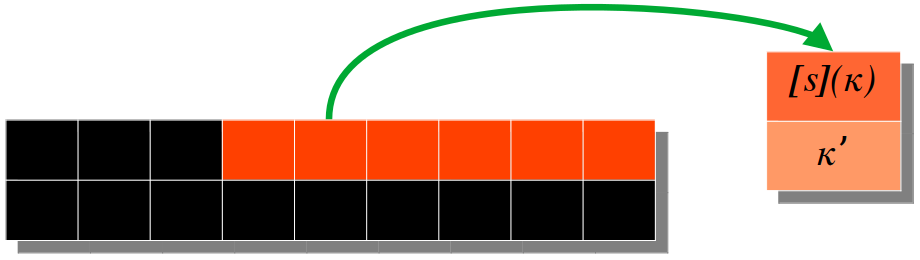
\includegraphics[width=1\linewidth]{conditional}

  \label{fig:qafny-con-analog}
\end{minipage}
\hfill
\begin{minipage}[t]{0.5\textwidth}
\subcaption{Mask/Unmask Function Modeling}
  \begin{mathpar}
    \inferrule[]{R \\ \Omega;\sigma;\varphi\models \theta \mapsto \sch{m}{z_j}{c_{j2}\,|c_{j1}\,\beta_j}}
          {\Omega;\sigma;\varphi\models \mathpzc{M}(b,\theta) 
              \mapsto \sch{m}{z_j}{c_{j1}.c_{j2}\,\beta_j}+q(\lambda,\neg b) }

    \inferrule[]{R
            \\\Omega;\sigma,\varphi\models \theta \mapsto \sch{m'}{z'_j}{c_{j1}.c'_{j2}\,\beta_j}+q(\lambda,\neg b)}
          {\Omega;\sigma,\varphi\models \mathpzc{U}(\neg b,\theta) \mapsto \sch{m}{z_j}{c_{j1}.c_{j2}\,\beta_j}+q(\lambda,\neg b)
  \\\\ \\ * \mathpzc{U}(b,\theta) \mapsto \sch{m'}{z'_j}{c'_{j2}\,|c_{j1}\,\beta_j} }
  \end{mathpar}

  \label{fig:qafny-mu-model}
\end{minipage}

{\begin{minipage}[t]{\textwidth}
\subcaption{Semantic/Proof Rules}
  \begin{mathpar}

\inferrule[SIF]{ R \\ FV(\emptyset,s)\subseteq \lambda'
          \\(\varphi[\lambda'\mapsto \sch{m}{z_j}{c_{j2}\,|c_{j1}\,\beta_j}],s) 
      \longrightarrow (\varphi[\lambda'\mapsto \sch{m'}{z'_j}{c'_{j2}\,|c_{j1}\,\beta_j}],s') } 
{(\varphi[\lambda\uplus\lambda'\mapsto \sch{m}{z_j}{c_{j1}.c_{j2}\,\beta_j}+q(\lambda,\neg b)],\sifq{b}{s}) \longrightarrow 
          (\varphi[\lambda\uplus\lambda'\mapsto \sch{m'}{z'_j}{c_{j1}.c'_{j2}\,\beta_j}+q(\lambda,\neg b)],\sifq{b}{s'}) }

    \inferrule[PIF]{\Omega;\{\lambda' : \tcht\} \vdash Q' \\ \fivepule{\Omega}{\sigma[\lambda' \mapsto \tcht]}{\mmode}{P[\mathpzc{M}(b,\lambda')/ \lambda \uplus \lambda']}{s}{Q * Q'}}
                {\fivepule{\Omega}{\sigma[\lambda \uplus \lambda' \mapsto \tcht]}{g}{P}{\sifq{b}{s}}{P[\mathpzc{U}(\neg b,\lambda \uplus \lambda')/\lambda \uplus \lambda')] * Q'[\mathpzc{U}(b,\lambda \uplus \lambda')/\lambda']}}

\mprset{flushleft}
    \inferrule[SLOOP]{ n_1 < n_2 }
                  {(\varphi,\sqwhile{j}{n_1}{n_2}{b}{s}) \longrightarrow \\\\ \quad (\varphi,\sseq{\sifq{b}{s}}{\sqwhile{j}{\texttt{S}\;n_1}{n_2}{b}{s})}}

    \inferrule[PLOOP]{n_1 < n_2\\ \fivepule{\Omega}{\sigma}{\mmode}{P(j)\wedge j \,\slt\, n_2}{\sifq{b}{s}}{P(\snext{j})} }
     {\fivepule{\Omega}{\sigma}{g}{P(n_1)}{ \sqwhile{j}{n_1}{n_2}{b}{s} }{P(n_2)} }

  \end{mathpar}

  \label{fig:qafny-mu-rules}
\end{minipage}
}
}
{\footnotesize
\[
\begin{array}{l}
\theta := q \mid \lambda
\\[0.2em]
q(\lambda,\neg b) = \schk{m}{z_k}{c_{k1}.c_{k2}\,\beta_k}
\;\;\texttt{where}\;\forall k.\;\slen{c_{k1}}=\slen{\lambda}\wedge \denote{\neg b[c_{k1}/\lambda]}
\\[0.2em]
R = FV(\emptyset,b)=\lambda \wedge \forall j.\; \slen{c_{j1}}=\slen{\lambda}\wedge\denote{b[c_{j1}/\lambda]}
\end{array}
\]
}
\caption{Semantic and Proof Rules for Conditionals and For-loops. $\theta$ is either a session or a quantum state. $\mathpzc{M}$ is the mask function and $\mathpzc{U}$ is the unmask function. }
\label{fig:exp-proofsystem-3}
\end{figure*}

\myparagraph{Rules for Conditionals and For-Loops}\label{sec:conditionals}
\Cref{fig:qafny-con-analog} describes the analogy of quantum conditionals in \qafny, which are partial map functions that only apply applications on the marked red parts and mask the marked black parts.
It contains two level of masking. For each basis state element in a state with session $\lambda_b\uplus \lambda_a$, it masks the $\lambda_b$ part of the state, i.e., if the state has the form: $\sch{m}{z_j}{c_{j1}.c_{j2}\beta_j}$ with $\slen{c_{j1}} = \slen{\lambda_b}$, we mask the $c_{j1}$ part by pushing it to a masked stack as $\sch{m}{z_j}{c_{j2}\,|\,c_{j1}\,\beta_j}$, which is described in preparing the pre-state of the upper-level transition in rule \textsc{SIF} (\Cref{fig:qafny-mu-rules}).
The second level of masking happens in selecting elements in the state by checking the Boolean condition $b$ on them.
The $R$ condition in rule\textsc{SIF} finishes such task for us.
Here, we split the state into two parts as $\sch{m}{z_j}{c_{j1}.c_{j2}\,\beta_j}+q(\lambda,\neg b)$, where the first part are all basis states satisfying $b$ since if we replace the variables in $b$ with $c_{j1}$, the evaluation $\denote{b[c_{j1}/\lambda]}$ returns true, while the second part $q(\lambda,\neg b)$ contains all basis states evaluated to false.
After the masking, we apply the application $s$ on each element in the selected states, install the results ($z'_j$ and $c'_{j2}$ back to the unmasked state, and result in $\sch{m'}{z'_j}{c_{j1}.c'_{j2}\,\beta_j}+q(\lambda,\neg b)$.
The result state number $m'$ might be different from the pre-state number $m$ because applications in $s$ might increase the state numbers such as applying a quantum diffusion operation.

To design a proof rule for such partial map, we develop the mask ($\mathpzc{M}$) and unmask ($\mathpzc{U}$) operations (\Cref{fig:qafny-mu-model}), both take a Boolean expression $b$ and a quantum state as the argument. $\mathpzc{M}$'s modeling materializes the masking mechanism above. For a state $\sch{m}{z_j}{c_{j1}.c_{j2}\,\beta_j}+q(\lambda,\neg b)$, we preserve the basis states satisfying $b$, as shown in the predicate $R$, remove the unsatisfied basis states $q(\lambda,\neg b)$, and push the bases $c_{j1}$ to state stacks.
Here, we do not need to input $\mathpzc{M}$ the session associated with $c_{j1}$, because we can learn it through $b$.
In the pre-condition manipulation of rule \textsc{PIF} (\Cref{fig:qafny-mu-rules}), we substitute $\lambda \uplus \lambda'$ with $\mathpzc{M}(b,\lambda')$. During the process, the type for the session in $\sigma$ is changed from $\lambda \uplus \lambda'$ in the bottom to $\lambda'$ in the upper level.
The unmask function $\mathpzc{U}$ assembles the result state of applying $s$ to the masked $\lambda$ state with the other parts hidden in the unmasked state (the part marked black in \Cref{fig:qafny-con-analog}). Function $\mathpzc{U}$ is usually appeared to be a pair with both $b$ and $\neg b$. In the post-condition manipulation, we substitute $\lambda \uplus \lambda'$ with $\mathpzc{U}(\neg b,\lambda \uplus \lambda')$ in $P$, representing the unchanged and masked state, substitute $\lambda'$ with $\mathpzc{U}(b,\lambda \uplus \lambda')$ in $Q'$, representing the result of applying $s$ on the unmasked part, and assemble them together through the separation operation $*$.
$\mathpzc{U}$'s modeling in \Cref{fig:qafny-mu-model} captures the assemble procedure by merging two $\mathpzc{U}$ constructs together.

Rules \textsc{SLOOP} and \textsc{PLOOP} are the semantic and proof rules for a for-loop, which is a repeat operation of conditionals in \qafny. The $P(j)$ is a loop invariant with $j$ being a variable. The case for $n_1 \ge n_2$ is given in \Cref{sec:newtype}. As an example, we show the proof for a loop-step in \Cref{fig:shorqafny}.

{\footnotesize
  \begin{mathpar}
\mprset{flushleft}
\inferrule[]{
   \inferrule[]
   { \inferrule[] {
    \fivepule{\Omega}{\sigma_2}{\mmode}{X(\snext{j}) * \{y[0..n]\}\mapsto C(j).1}{ s }{X(\snext{j}) * \{y[0..n]\}\mapsto C'(j).1} }
  { \fivepule{\Omega}{\sigma_2}{\mmode}{X(\snext{j}) * \mathpzc{M}(b,\{y[0..n]\})\mapsto 0.C(j)+1.C(j)}{ s }{X(\snext{j}) * \{y[0..n]\}\mapsto C'(j).1} } }
   {  \Omega,\sigma_1\vdash_{\mmode} \{X(\snext{j}) * \{x[0..\snext{j}],y[0..n]\}\mapsto 0.C(j)+1.C(j)\} \sifq{x[j]}{s}
     \\\\\qquad\qquad \{ X(\snext{j}) * \mathpzc{U}(\neg x[j],\{x[0..\snext{j}],y[0..n]\})\mapsto 0.C(j)
          * \mathpzc{U}(x[j],\{x[0..\snext{j}],y[0..n]\})\mapsto C'(j).1\}
     } } {
\fivepule{\Omega}{\sigma}{\mmode}{X(j) * \{x[0..j],y[0..n]\}\mapsto C(j)}{ \sifq{x[j]}{s} }{X(j\,\sminus\,1) * \{x[0..\snext{j}],y[0..n]\} \mapsto 0.C(j)+1.C'(j)} }
  \end{mathpar}
{\hspace*{-1.5em}
$\begin{array}{l}
X(j)=\shad{2^{n \,\sminus\,  j}}{n \,\sminus\, j}{}
\quad
C(j)=\sch{2^k}{\frac{1}{\sqrt{2^k}}}{\tos{j}^{k}.\tos{a^{\tos{j}^k}\;\%\;N}}
\quad
i.C(j)=\sch{2^{\snext{k}}}{\frac{1}{\sqrt{2^{\snext{k}}}}}{\tos{j}^k.i.\tos{a^{\tos{j}^k}\;\%\;N}}
\\
C'(j).i=\sch{2^{\snext{k}}}{\frac{1}{\sqrt{2^{\snext{k}}}}}{\tos{a^{\tos{j}^k.1}\;\%\;N}\,|\,\tos{j}^k.i}
\qquad
i.C'(j)=\sch{2^{\snext{k}}}{\frac{1}{\sqrt{2^{\snext{k}}}}}{\tos{j}^k.i.\tos{a^{\tos{j}^k.1}\;\%\;N}}
\\
\sigma_1=\{x[0..n\,\sminus\,\snext{j}] \mapsto \thadt, \{x[0..\snext{j}],y[0..n]\} \mapsto \tcht \}
\quad
\sigma=\{x[0..n\,\sminus\,\snext{j}] \mapsto \thadt, y[0..n] \mapsto \tcht \}
\quad
s=\ssassign{y}{}{a^{2^j}y\;\%\; N}
\end{array}$
}
}

The proof is built from bottom up. We first cut the $\thadt$ type state into two sessions ($x[0..n\,\sminus\,\snext{j}]$ and $x[j]$), join $x[j]$ with session $\{x[0..j],y[0..n]\}$, and double the state elements to be $0.C(j)+1.C(j)$, which is proved by applying the consequence rules. Notice that the type environment is also transitioned from $\sigma$ to $\sigma_1$.
By the same strategy of the $\mathpzc{U}$ rule in \Cref{fig:qafny-mu-model}, we combine the two $\mathpzc{U}$ terms into the final result. 
The second step applies rule \textsc{PIF} to substitute session $\{x[0..\snext{j}],y[0..n]\}$ with the mask construct $\mathpzc{M}(b,\{y[0..n]\})$ in the pre-condition and create two $\mathpzc{U}$ terms in the post-condition. The step on the top applies the modulo multiplication on every element in the masked state $\mapsto C(j).1$ by rule \textsc{PA-CH}.

\begin{figure*}[t]
{\footnotesize
\begin{minipage}[t]{0.4\textwidth}
\subcaption{Measurement Analogy}
  \vspace{0.5cm}
  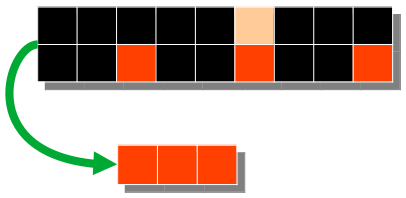
\includegraphics[width=1\linewidth]{measure}

  \label{fig:qafny-mea-analog}
\end{minipage}
\hfill
\begin{minipage}[t]{0.5\textwidth}
\subcaption{Measurement Modeling}
  \begin{mathpar}
    \inferrule[]{\Omega;\sigma;\varphi\models \theta \mapsto \theta'}
          {\Omega;\sigma;\varphi\models \mathpzc{F}(x,n,\theta) \mapsto \mathpzc{F}(x,n,\theta') }

    \inferrule[]{\slen{c}=n \\
           \Omega;\sigma;\varphi\models \theta \mapsto 
                      \sch{m}{\frac{z_j}{\sqrt{r}}}{c_{j}} \wedge x = (r,\tov{c})}
          {\Omega;\sigma,\varphi\models \mathpzc{F}(x,n,\theta) \mapsto \sch{m}{z_j}{c.c_{j}}+q(n,\neq c) }
  \end{mathpar}

  \label{fig:qafny-mea-model}
\end{minipage}

{\begin{minipage}[t]{\textwidth}
\subcaption{Semantic/Proof Rules}
  \begin{mathpar}

    \inferrule[SMea]{\varphi(y) = \{y[0..n]\uplus\lambda\mapsto \sch{m}{z_j}{c.c_{j}}+q(n,\neq c)\}}{(\varphi,\sexp{x}{\smea{y}}{s}) \longrightarrow (\varphi[\lambda \mapsto  \sch{m}{\frac{z_j}{\sqrt{r}}}{c_{j}}],s[(r,\tov{c})/x]) }

    \inferrule[PMea]{\fivepule{\Omega[x\mapsto \mmode]}{\sigma[\lambda\mapsto \tcht]}{\cmode}{P[\mathpzc{F}(x,n,\lambda)/y[0,n]\uplus\lambda]}{s }{Q} }
     {\fivepule{\Omega[y\mapsto \qmode{n}]}{\sigma[y[0,n]\uplus\lambda\mapsto \tcht]}{\cmode}{P}{\sexp{x}{\smea{y}}{s} }{Q} }

  \end{mathpar}

  \label{fig:qafny-mea-rules}
\end{minipage}
}
}
{\footnotesize
\[r= \sum_{k=0}^{m} \slen{z_k}^2
\qquad\qquad
q(n,\neq c) = \schk{m'}{z'_k}{c'.c'_{k}} \;\;\texttt{where}\;c'\neq c\]
}
\caption{Semantic and Proof Rules for Measurement. $\mathpzc{F}$ is the measurement function construct. $\tov{c}$ turns bitstring $c$ to an integer, and $r$ is the likelihood that the bitstring $c$ appears in a basis state. }
\label{fig:exp-proofsystem-4}
\end{figure*}

\myparagraph{Rules for Measurement}\label{sec:measurement}
As \Cref{fig:qafny-mea-analog} describes, quantum measurement is a two-step array filter: 1) each element in the state is partitioned into two parts, and we select a first part of an element as a key, as shown in the marked pink part; and 2) we create a new array state by removing all the first parts in the old state and collecting the elements whose first part is equal to the key.
The second step actually collects elements in a periodical manner as shown in the analogy in \Cref{fig:qafny-mea-analog}, where the marked red basis states appear in a periodical pattern in the whole state. This behavior is universally true for quantum operations, and many quantum algorithms utilize the periodical pattern of quantum computation.

In rule \textsc{SMea}, we pick an $n$-length bitstring $c$ as the marked pink key, and elect $m$ basis states $\sch{m}{z_j}{c.c_{j}}$ that has the key $c$. In the post-state, we update the remaining session $\lambda$ to $\sch{m}{\frac{z_j}{\sqrt{r}}}{c_{j}}$ with the adjustment of amplitude $\frac{1}{\sqrt{r}}$, and replace the variable $x$ in the statement $s$ with the value $(r,\tov{c})$.
In designing the proof rule \textsc{PMea}, the operation $\mathpzc{F}(x,n,\lambda)$ is invented,
whose modeling is in \Cref{fig:qafny-mea-model}, to do exactly the two steps above by selecting an $n$-length prefix bitstring $c$ in a basis state, computing the probability $r$, and assigning $(r,\tov{c})$ to variable $x$.
Rule \textsc{PMea} in \Cref{fig:qafny-mea-rules} replaces the session $y[0..n]\cup \lambda$ in $P$ with the measurement result session $\mathpzc{F}(x,n,\lambda)$ and updates the type state $\Omega$ and $\sigma$. 

{\footnotesize
  \begin{mathpar}
\inferrule[]{
   \inferrule[]
   { \fivepule{\Omega[u\mapsto \mmode]}{\sigma[\lambda \mapsto \tcht]}{\mmode}{\mathpzc{F}(u,n,x[0..n])\mapsto C'}{ \{\} }{x[0..n] \mapsto D * E} }
   { \fivepule{\Omega}{\sigma}{\mmode}{\{y[0..n],x[0..n]\}\mapsto C'}{ \sexp{u}{\smea{y}}{\{\}} }{x[0..n] \mapsto D * E}
     } } {\fivepule{\Omega}{\sigma}{\mmode}{\{x[0..n],y[0..n]\}\mapsto C}{ \sexp{u}{\smea{y}}{\{\}} }{x[0..n] \mapsto D * E} }
  \end{mathpar}
{\hspace*{-1em}
$\begin{array}{l}
C=\sch{2^{n}}{\frac{1}{\sqrt{2^{n}}}}{\tos{j}.\tos{a^{j}\;\%\;N}}
\quad
C'=\sch{2^{n}}{\frac{1}{\sqrt{2^{n}}}}{\tos{a^{j}\;\%\;N}.\tos{j}}
\quad
\sigma=\{\{x[0..\snext{j}],y[0..n]\}:\tcht\}
\\
D=\smch{\frac{1}{\sqrt{s}}}{s}{t\,\splus\,k p}
\quad
E=p = \texttt{ord}(a,N)
\wedge
u=(\frac{s}{2^n},a^{t}\;\%\;N)
\wedge
s=\texttt{rnd}(\frac{2^n}{p})
\end{array}$
}
}

For an instance, we show a proof fragment above for the partial measurement in line 11 in \Cref{fig:shorqafny}.
The bottom two lines are to modify the array group order of the session from 
$\{y[0..n],x[0..n]\}$ to $\{x[0..n],y[0..n]\}$ through the consequence rule of state equivalence.
The second line proof, applies rule $\textsc{PMea}$ by replacing session $\{x[0..n],y[0..n]\}$ with $\mathpzc{F}(u,n,x[0..n])$.
On the top statement, the pre- and post-conditions are equivalent, because of the periodical aspects in quantum computing.
In session $\{y[0..n],x[0..n]\}$, group $y[0..n]$ stores the basis state $\tos{a^{j}\;\%\;N}$, which contains value $j$ that represents the basis states for group $x[0..n]$. Selecting a basis state $a^{t}\;\%\;N$ also filters the $j$ in $x[0..n]$, which refers to any values $j$ having the relation $a^{j}\;\%\;N=a^{t}\;\%\;N$. Notice that modulo multiplication is a periodical function, which means that the relation can be rewritten $a^{t+kp}\;\%\;N=a^{t}\;\%\;N$, such that $p$ is the period order. Thus, the $x[0..n]$ state is rewritten as a summation of $k$: $\smch{\frac{1}{\sqrt{s}}}{s}{t\,\splus\,k p}$. The probability of selecting $\tos{a^{j}\;\%\;N}$ is $\frac{s}{2^n}$.
In \qafny, we set up additional axioms for representing these periodical manners, which is why the pre- and post-condition equivalence is granted.

\begin{figure*}[t]
{\footnotesize
\begin{minipage}[t]{0.35\textwidth}
\subcaption{Diffusion Analogy}
  \vspace{0.5cm}
  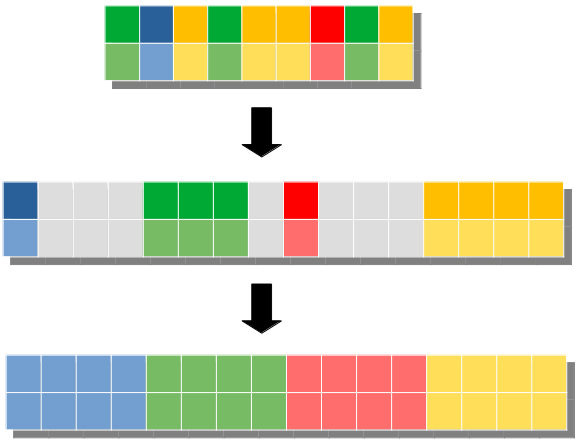
\includegraphics[width=1\linewidth]{diffuse}

  \label{fig:qafny-dis-analog}
\end{minipage}
\hfill
\begin{minipage}[t]{0.6\textwidth}
\subcaption{Diffusion Modeling}
  \begin{mathpar}
    \inferrule[]{\Omega;\sigma;\varphi\models \theta \mapsto \theta'}
          {\Omega;\sigma;\varphi\models \mathpzc{D}(n,\theta) \mapsto \mathpzc{D}(n,\theta') }

    \inferrule[]{\Omega;\sigma;\varphi\models \theta\mapsto \mathpzc{D'}(n,\sch{n'}{z_{i}}{c_{i}})}
          {\Omega;\sigma;\varphi\models \mathpzc{D}(n,\theta) \mapsto \schii{n'}{z_{i}}{c_{i}} }

    \inferrule[]{\slen{\tos{j}}=n
   \\ \Omega;\sigma;\varphi\models \theta\mapsto \Msum_{j=0}^{m}\schk{2^n}{(2 z_{jk}\sum_{t=0}^{2^n}z_{jt} - z_{jk})}{\tos{k}.c_{jk}}}
          {\Omega;\sigma;\varphi\models \theta \mapsto \mathpzc{D'}(n,\Msum_{j=0}^{m}\schk{2^{n}}{z_{jk}}{\tos{k}.c_{jk}}) }
  \end{mathpar}

  \label{fig:qafny-dis-model}
\end{minipage}

{\begin{minipage}[t]{\textwidth}
\subcaption{Semantic/Proof Rules}
  \begin{mathpar}

    \inferrule[SDis]{FV(\Omega,l)=\lambda \\ \varphi(\lambda) = \{\lambda\uplus\lambda'\mapsto q\}}
      {(\varphi,\ssassign{l}{}{\sdis}) \longrightarrow (\varphi[\lambda\uplus\lambda' \mapsto \mathpzc{D}(\slen{\lambda},q)],\{\}) }

    \inferrule[PDis]{ FV(\Omega,l)=\lambda\\\sigma(\lambda)=\{\lambda\uplus\lambda:\tcht\} }
     {\fivepule{\Omega}{\sigma}{g}{P[\mathpzc{D}(\slen{\lambda},\lambda\uplus\lambda')/\lambda\uplus\lambda']}{\ssassign{l}{}{\sdis} }{P} }

  \end{mathpar}

  \label{fig:qafny-dis-rules}
\end{minipage}
}
}
\caption{Semantic and Proof Rules for Diffusion Operations. $\mathpzc{D}$ models the diffusion operations. }
\label{fig:exp-proofsystem-5}
\end{figure*}

\myparagraph{Rules for Diffusion}\label{sec:diffuse}
Quantum diffusion operations ($\ssassign{l}{}{\sdis}$) reorient the amplitudes of basis states based on the basis state corresponding to $l$. They are analogized to an aggregate operation of reshape and mean computation, both appeared in many programming languages \footnote{Such as Python}.
The aggregate operation first applies a reshape, where elements are regrouped into a normal form, as the first agree of \Cref{fig:qafny-dis-analog}. More specifically, the diffusion modeling function $\mathpzc{D}(n,\theta)$ takes an $n'$-element state $\sch{n'}{z_{j}}{c_{j}}$ as the second rule in \Cref{fig:qafny-dis-model}. The $n$ number corresponds to the number of bits in the session potion matching $l$.
Then, we rearrange the state by a helper function $\mathpzc{D'}$ by extending the element number from $n'$ to $m*n$ with probably adding new elements that originally have zero amplitude (the marked white elements in \Cref{fig:qafny-dis-analog}), as the third rule in \Cref{fig:qafny-dis-model}.
Here, let's view a basis $c_{i}$ as a small-endian (LSB) number $\tov{c_{i}}$. The rearrangement of changing bases $c_{i}$ (for all $i$) to $\tos{k}.c_{jk}$ is analogized to rearranging a number $\tov{c_{i}}$ to become the form $2^n j+k$, with $k\in [0,2^n)$. 
Basically, the reshape step rearranges the basis states to be placed in a periodical counting sequence, with $2^n$ being the order.

The mean computation analogy (the second arrow in \Cref{fig:qafny-dis-analog}) takes every period in the reshaped state, and for each basis state, we redistribute the amplitude by the formula $(2 z_{jk}\sum_{t=0}^{2^n}z_{jt} - z_{jk})$.
In another word, for each period, given a basis state $k$, we sum all the amplitudes from $0$ to $2^n$ in the period as $z_{sum}$, then the redistributed amplitude for $k$ is $2 z_k z_{sum}-z_k$. 

Rule \textsc{SDis} is the semantics for diffusion $\ssassign{l}{}{\sdis}$, which applies the $\mathpzc{D}$ function to the session $\lambda \uplus \lambda'$, where $\lambda$ corresponds to the $l$'s session. Proof rule \textsc{PDis} replaces session $\lambda\uplus \lambda'$ with the application $\mathpzc{D}$ on the session.
Quantum diffusion operations are used in many algorithms, such as amplifying a basis state's amplitude value in Grover's search algorithm, or redistributing a possible path direction in quantum walk algorithm.
In these algorithms, the session piece that is diffused has either a small constant number of qubits or the whole session, meaning that the $n$ number in the $\mathpzc{D}$ function is either very small or equal to $\slen{\lambda \uplus \lambda'}$, as the whole session.
In either case, the summation formula in $\mathpzc{D}$'s modeling (\Cref{fig:qafny-dis-model}) can be rewritten as very few terms that facilitate the automated verification, which is exactly how we handle the diffusion operations in \qafny.
An example of Grover's search and quantum walk algorithm is given in \Cref{sec:arith-oqasm}.

\subsection{\qafny Metatheory}\label{sec:theorems}

The type system is sound and the proof system is proved to be sound and complete.


\myparagraph{Type Soundness}
We prove that well-typed \qafny programs are well defined; i.e., the
type system is sound with respect to the semantics. 
We begin by defining the session domain and state well-formedness.

\begin{definition}[Well-formed session domain]\label{def:well-formed-ses}\rm 
  A type environment $\sigma$'s session domain is \emph{well-formed}, written
  $\Omega \vdash \dom{\sigma}$, iff for every session $\lambda\in \dom{\sigma}$:
\begin{itemize}
\item $\lambda$ is disjoint unioned, i.e., for every two ranges $x[i..j]$ and $y[i'..j']$, $x[i..j]\cap y[i'..j']=\emptyset$.

\item For every range $x[i..j]\in\lambda$, $\Omega(x)=\qmode{n}$ and $[i,j) \subseteq [0,n)$.
\end{itemize}
\end{definition}

\begin{definition}[Well-formed \qafny state]\label{def:well-formed}\rm 
  A state $\varphi$ is \emph{well-formed}, written
  $\Omega;\sigma \vdash \varphi$, iff $\dom{\sigma} = \dom{\varphi}$, $\Omega\vdash\dom{\sigma}$, and:
\begin{itemize}
\item For every $\lambda \in \sigma$ such that $\sigma(\lambda) = \tnort$, $\varphi(\lambda)=\ket{c}$ and $\slen{c}=\slen{\lambda}$.

\item For every $\lambda \in \sigma$ such that $\sigma(\lambda) = \thadt$, $\varphi(\lambda)=\shad{2^n}{n}{\alpha(r_j)}$ and $\slen{\lambda}=n$.

\item For every $\lambda \in \sigma$ such that $\sigma(\lambda) = \tcht$, $\varphi(\lambda)=\sch{m}{z_j}{c_j\,\beta_j}$ and $\slen{\lambda}=\slen{c_j}$ for all $j$.
\end{itemize}
\end{definition}

The \qafny type soundness is stated as two theorems, type progress and preservation theorems. The proofs are done by induction on \qafny statements $s$ and mechanized in Coq. Type progress states that any well-typed \qafny program can take a move, while type preservation states that for any such move, the transitioned type and state are preserved and well-typed, respectively.

\begin{theorem}[\qafny type progress]\label{thm:type-progress-oqasm}\rm 
If $\Omega;\sigma \vdash_g s \triangleright \sigma'$ and $\Omega;\sigma \vdash \varphi$, then either $s=\{\}$, or there exists $\varphi'$ and $s'$ such that $(\varphi,s)\longrightarrow (\varphi',s')$.
\end{theorem}

\begin{theorem}[\qafny type preservation]\label{thm:type-preservation-oqasm}\rm 
If $\Omega;\sigma \vdash_g s \triangleright \sigma'$, $\Omega;\sigma \vdash \varphi$, and $(\varphi,s)\longrightarrow (\varphi',s')$, then 
there exists $\Omega'$ and $\sigma''$, $\Omega';\sigma'' \vdash_g s' \triangleright \sigma'$ and $\Omega';\sigma'' \vdash \varphi'$.
\end{theorem}

\myparagraph{Proof System Soundness and Completeness}
We prove that the \qafny proof system is well defined; i.e., any properties derived in the \qafny proof system for well-typed \qafny programs can be interpreted by the state transitions in the \qafny semantics.
In \qafny, there are three different state representations for a session $\lambda$ and two sessions can be joined into a large session.
Hence, given a statement $s$ and an initial state $\varphi$, the semantic transition $(\varphi,s) \longrightarrow^{*} (\varphi',\{\})$ might not be unique, in the sense that there might be different representations of $\varphi'$, due to the different state representations.
However, any $\tnort$ and $\thadt$ type state can be represented as a $\tcht$ type state, so that $\tcht$ type states can be viewed as the \emph{most general} state representation. We also have state equivalence relations defined for capturing the behaviors of session permutation, join and split. We define a \emph{most general state representation} of evaluating a statement $s$ in an initial state $\varphi$ below.

\begin{definition}[Most general \qafny state]\label{def:most-gen}\rm 
  Given a statement $s$, an initial state $\varphi$, kind environment $\Omega$, type environment $\sigma$, and context mode $g$, such that $\Omega;\sigma\vdash \varphi$, $\vdash_g s \triangleright \sigma^*$, $\Omega;\sigma[\uparrow \sigma^*]\vdash \varphi^*$, and $(\varphi,s) \longrightarrow^{*} (\varphi^*,\{\})$, $\varphi^*$ is the most general state representation of evaluating $(\varphi,s)$, iff for all $\sigma'$ and $\varphi'$, such that $\vdash_g s \triangleright \sigma'$, $\Omega;\sigma[\uparrow \sigma']\vdash \varphi'$ and $(\varphi,s) \longrightarrow^{*} (\varphi',\{\})$, $\sigma' \preceq \sigma^*$ and $\varphi' \equiv \varphi^*$.
\end{definition}

The \qafny proof system correctness is defined by the soundness and relatively completeness theorems below, which has been formalized and proved in Coq. The \qafny proof system only describes the quantum portion of the whole Qafny+Dafny system, and the quantum portion contains non-terminated programs. Hence, the soundness and completeness essentially refers to the partial correctness of the \qafny proof system and the total correctness is achieved by the Qafny+Dafny system through mapping \qafny to Dafny, i.e., a separation logic proof system. Essentially, the \qafny proof system correctness is defined in terms of programs being well-typed. The type soundness theorem suggests that any intermediate transitions of evaluating a well-typed \qafny program is also well-typed. Thus, we can conclude that the pre- and post- conditions of a program are modeled properly through the above modeling rules that rely on well-typed transition states.

\begin{theorem}[proof system soundness]\label{thm:proof-soundness}\rm 
For a well-typed program $s$, such that $\Omega;\sigma\vdash_g s \triangleright \sigma'$, $\fivepule{\Omega}{\sigma}{g}{P}{s}{Q}$, $\Omega;\sigma;\varphi\models P$, then there exists a state representation $\varphi'$, such that $(\varphi,s)\longrightarrow (\varphi',\{\})$ and $\Omega;\sigma[\uparrow\sigma'];\varphi'\models Q$, and there is a most general state representation $\varphi^*$ of evaluating $(\varphi,s)$ as $(\varphi,s)\longrightarrow (\varphi^*,\{\})$ and $\varphi' \equiv \varphi*$.
\end{theorem}

\begin{theorem}[proof system relative completeness]\label{thm:proof-completeness}\rm 
For a well-typed program $s$, such that $\Omega;\sigma\vdash_g s \triangleright \sigma'$, $(\varphi,s)\longrightarrow (\varphi',\{\})$ and $\Omega;\sigma\vdash \varphi$, there is most general state representation $\varphi^*$, such that $(\varphi,s)\longrightarrow (\varphi',\{\})$ and $\varphi' \equiv \varphi^*$ and $\Omega;\sigma\vdash_g s \triangleright \sigma^*$ and $\Omega;\sigma[\uparrow \sigma^*]\vdash \varphi^*$, and there are predicates $P$ and $Q$, such that $\Omega;\sigma;\varphi\models P$ and $\Omega;\sigma[\uparrow\sigma^*];\varphi^* \models Q$ and $\fivepule{\Omega}{\sigma}{g}{P}{s}{Q}$.
\end{theorem}





%\section{Key Features through A Running Example}
\label{sec:shors}

\begin{figure}[t]
{\small
\[\hspace*{-1em}
\begin{array}{r l  l}
\textcolor{blue}{1}
&&
\{A(x) * A(y) * B \}
\quad\text{where}\;\;
A(\beta) = \beta[0..n] \mapsto \ket{\overline{0}} 
\\[0.2em]
&&
\qquad\qquad\qquad
\qquad\qquad\quad
\begin{array}{l}
B = 1 < a < N \wedge n > 0 \;\wedge
\\\qquad N < 2^n \wedge \texttt{gcd}(a,N)=1
\end{array}
\\[0.5em]
\textcolor{blue}{2}
&
&
\textcolor{teal}{
\Rightarrow
\{\dabs{\ihadh}(x[0..n]) \mapsto C * A(y) * B \}
}
\\[0.2em]
&&
\qquad\qquad\qquad
\qquad\;\;
\text{where}
\;\;
\textcolor{teal}{
C = \shad{2^n}{n}{}
}
\\[0.5em]
\textcolor{blue}{3}
& \ssassign{x}{}{\ihadh};
&
\textcolor{teal}{
\{x[0..n] \mapsto C * A(y) * B \}
}
\\[0.4em]
\textcolor{blue}{4}
&
&
\textcolor{teal}{
\Rightarrow
\{x[0..n] \mapsto C * \dabs{y\splus 1}(y[0..n]) \mapsto \ket{\overline{0}.1} * B \}
}
\\[0.4em]
\textcolor{blue}{5}
& \ssassign{y}{}{y\splus 1};
&
\textcolor{teal}{
\{x[0..n] \mapsto C * y[0..n] \mapsto \ket{\overline{0}.1} * B \}
}
\\[0.4em]
\textcolor{blue}{6}
& 
&
\textcolor{teal}{
\Rightarrow
\{ E(0) * B \}
}
\;\;
\texttt{where}\;\;
\textcolor{teal}{E(k) =}
\\[0.2em]
&&
\qquad\qquad\quad\;
\qquad
\textcolor{teal}{
\begin{array}{l}
x[0..n\,\sminus\,k] \mapsto \shad{2^{n \,\sminus\,  k}}{n \,\sminus\, k}{}\;*
\\[0.2em]
\{x[0..k],y[0..n]\} \mapsto \sch{2^k}{\frac{1}{\sqrt{2^k}}}{\tos{j}.\tos{a^{j}\;\%\;N}}
\end{array}
}
\\[0.4em]
\textcolor{blue}{7}
&\sqforh{\sint{j}{0}}{j\,\slt\, n}{x[j]}{\dplus{j}}
&
\{E(j) * B \}
\\[0.4em]
\textcolor{blue}{8}
&
\{\quad  \ssassign{y}{}{a^{2^j}y\;\%\; N}
&
\textcolor{teal}{
\{E(j\,\splus\, 1) * B \}
}
\\[0.4em]
\textcolor{blue}{9}
&
\}
&
\textcolor{teal}{
\{E(n) * B \}
}
\\[0.4em]
\textcolor{blue}{10}
&
&
\textcolor{teal}{
\Rightarrow
\{\{x[0..n],y[0..n]\} \mapsto \sch{2^{n}}{\frac{1}{\sqrt{2^{n}}}}{\tos{j}.\tos{a^{j}\;\%\;N}} * B \}
}
\\[0.4em]
\textcolor{blue}{11}
& \sexp{u}{\smea{y}}{...}
&
\textcolor{purple}{
\big{\{}
\begin{array}{l}
x[0..n] \mapsto \smch{\frac{1}{\sqrt{s}}}{s}{t\,\splus\,k p} 
\wedge
p = \texttt{ord}(a,N)
\\
\wedge\;
\texttt{nat}(u)=a^{t}\;\%\;N
\wedge
s=\texttt{rnd}(\frac{2^n}{p}) \wedge B
\end{array}
\big{\}}
}
\end{array}
\]
}
\caption{First half of the Shor's algorithm quantum part. Second half in \Cref{fig:shorqafny2}. $\snat{u}$ gets the integer number part of $u$ (mode $\mmode$). $\sord{a,N}$ gets the order of $a$ and $N$. $\srnd{r}$ rounds $r$ to the nearest integer. }
\label{fig:shorqafny}
\end{figure}

As an illustration of QNP, we implement and prove part of the Shor's algorithm in \Cref{fig:shorqafny}.
Given an integer $N$, Shor's algorithm finds its nontrivial prime factors, which has the following step: (1) randomly pick a number $1 < a < N$ and compute $k=\texttt{gcd}(a,N)$ \footnote{compute the greatest common divisor of $a$ and $N$}; (2) if $k \neq 1$, $k$ is the factor; (3) otherwise, $a$ and $N$ are coprime and we find the order $p$ of $a$ and $N$ \footnote{the order $p$ is the smallest number such that $a^p \% N = 1$}; (4) if $p$ is even and $a^{\frac{p}{2}} \neq -1 \% N$, $\texttt{gcd}(a^{\frac{p}{2}}\pm 1,N)$ are the factors, otherwise, we repeat the process. Step (2) is the quantum part of Shor's algorithm and \Cref{fig:shorqafny} and \Cref{fig:shorqafny2} show its automated proof in QNP. In \Cref{fig:shorexample}, we show the actual implementation and proof in the Qafny tool.

\begin{wrapfigure}{r}{8.2cm}
  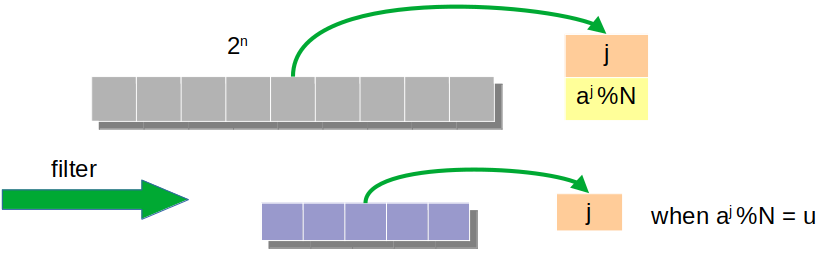
\includegraphics[width=.60\textwidth]{shorsmap}
  \caption{The array analogy of Shor's first half in \Cref{fig:shorqafny}. }
\label{fig:shorsanalog}
\end{wrapfigure}

The Shor's quantum first half in \Cref{fig:shorqafny} can be analogized as an efficient array filter operation.
The steps before line 11 (steps at line 3, 4 and 7-9) create a $2^n$-length of pairs, each of which is formed as $(j,a^j \% N)$ where $j\in [0,2^n)$. The measurement in line 11 filters the array as a new one ($x$) with all elements $j$ satisfying $a^j \% N=z$ where $z$ is a randomly picked number. Notice that modulo multiplication $f(j)=a^j\%N$ is a periodic function. All elements in $x$ satisfy $a^j \% N=z$, which means that 1) there will be a smallest $t$ such that $a^t \% N=z$, and 2) all elements can be rewritten as $j=t+kp$ and $p$ is the period of the modulo multiplication function because $a^{t+kp} \% N=z$, which is given as the post-condition on the right of line 11.
The first half implementation and correctness proof in \Cref{fig:shorqafny} exactly reflects the array analogy aspect.
One of the biggest advantage of using \qafny is that we can analogize quantum operations to classical array operations, so that we can utilize the existing automated proof infrastructure in many tools, such as Dafny.
In the Qafny implementation, verifying a quantum program usually requires only the user input of the pre-, post-, and loop invariant. For example, the proof of \Cref{fig:shorqafny} in \qafny requires none of the states marked teal, but only the conditions marked black and purple. \footnote{The purple is also not needed if we combine the Shor's first and second half algorithms together.}
Here, we step by step discuss the states, program syntax, and proofs of the aspect.

\begin{figure}[t]
{
  \small
\[\hspace*{-0.5em}
\begin{array}{l}
\textcolor{blue}{\text{Basic Terms:}}\\[0.2em]
\begin{array}{llcl llcl llcl}
\text{Nat. Num} & m, n & \in & \mathbb{N}
&
      \text{Real} & r & \in & \mathbb{R}
&
      \text{Complex Number} & z & \in & \mathbb{C}
\\
      \text{Variable} & x,y &&

 & \text{Bit} & d & ::= & 0\mid 1       
&
      \text{Bitstring} & c & \in & d^{+}      
\\
\text{Phase} & \alpha(r) & ::= & e^{2\pi i r}
\\
\end{array}
\\[1em]
\textcolor{blue}{\text{Modes, Kinds, Types, and Classical/Quantum Values:}}\\[0.2em]
\begin{array}{llclll} 
      \text{Mode} & g & ::= & \cmode  \mid \mmode\\
      \text{Classical Value} & v & ::= & n \mid (r,n)\\
      \text{Full Mode (Kind)} & \overline{g} & ::= & g \mid \qmode{n} \\
      \text{Quantum Type} & \tau & ::= & \tnort &\mid \thadt & \mid \tcht \\
      \text{Quantum Value} & q & ::= & \ket{c} & \mid \shad{2^n}{n}{\alpha(r_j)} &\mid \sch{m}{z_j}{c_j \,\beta_j} \\
    \end{array}
\\[1em]
\textcolor{blue}{\text{Quantum Sessions, Environment, and States}}\\[0.2em]
\begin{array}{llclcl} 
      \text{Range} & l & ::= & x[n..m] \\
      \text{Session} & \lambda & ::= & \overline{x[n..m]} & \text{by} & \uplus \\
      \text{Type Environment} & \sigma & ::= & \overline{\lambda : \tau } & \text{by} & \cup \\
      \text{Quantum State} & \varphi & ::= & \overline{ \lambda : q } & \text{by} & \cup \\
    \end{array}
\end{array}
  \]
}
  \caption{\qafny element syntax. Each range $x[n..m]$ in a session $\overline{x[n..m]}$ represents the number range $[n,m)$ in a qubit array $x$. Sessions are finite lists, while type environments and states are finite sets. the operations after "by" refer to the concatenation operations for session, type environments and quantum states. }
  \label{fig:qafny-state}
\end{figure}

\myparagraph{Classical and Quantum States}
On the right of \Cref{fig:shorqafny} line 1, it is the the pre-condition of the program, which describes two quantum arrays; both are initialized to be $n$-qubit of bits $0$ (as $\overline{0}$), represented as predicates $A(x)$ and $A(y)$, and other restrictions for integers $a$ and $N$ represented as predicate $B$.
In Qafny, there are three kinds of values, two of which are classical ones represented by the two modes: $\cmode$ and $\mmode$ in \Cref{fig:qafny-state}. The former represents classical values, represented as a natural number $n$, that do not intervene with quantum measurements and are evaluated in the compilation time, the latter represents values, represented as a pair $(r,n)$, produced from a quantum measurement. The real number $r$ is a characteristic representing the theoretical probability of the measurement resulting in the natural number value $n$. In \Cref{fig:shorqafny}, $a$ and $N$ are $\cmode$-mode values and $u$ is a $\mmode$ value so that we can use function $\texttt{nat}$ to produce its natural number part. Quantum values are defined in the units of qubit arrays that represent potentially entangled qubit clusters and are represented as kind $\qmode{n}$, where $n$ is the array size. \qafny represents qubit arrays as \emph{sessions} ($\lambda$), which consist of different \emph{disjoint ranges}, each of which describes an array fragment $x[n..m]$, where $x$ is a variable representing a qubit array piece, named a qubit group, initialized by an \texttt{init} statement, and $[n..m]$ represents the array fragment from position $n$ to $m$ (exclusive) in group $x$.
For simplicity, we assume that there are no aliasing array piece variables in this paper, i.e., two distinct variables represent disjoint array pieces. For example, $\{\{x[0..n],y[0..n]\}$ in \Cref{fig:shorqafny} line 10 represents a $2n$ qubit array containing two disjoint pieces $x[0..n]$ and $y[0..n]$ referring to the ranges $[0,n)$ in groups $x$ and $y$, respectively.
We also abbreviate a singleton session $\{x[n..m]\}$ as a range $x[n..m]$.

Each length-$n$ session is associated to a quantum state with the same length that can be one of the three forms ($q$ in \Cref{fig:qafny-state}) that are corresponding to three different types ($\tau$ in \Cref{fig:qafny-state}). 
A $\tcht$-type session has state form $\sch{m}{z_j}{c_j\,\beta_j}$, which is the most general quantum state representation and is designed as an analogy to classical arrays in the sense that each quantum state basis is viewed as an individual array element that does not Intervene with other elements.
For example, In \Cref{fig:shorqafny} line 10, session $\{\{x[0..n],y[0..n]\}$ has state $\sch{2^{n}}{\frac{1}{\sqrt{2^{n}}}}{\tos{j}.\tos{a^{j}\;\%\;N}}$, represented as a $2^n$ entanglement array, whose element is a triple of an amplitude $\frac{1}{\sqrt{2^{n}}}$, a basis $\tos{j}.\tos{a^{j}\;\%\;N}$ \footnote{$\tos{j}.\tos{a^{j}\;\%\;N}$ can be split into $\tos{j}$ and $\tos{a^{j}\;\%\;N}$ -- both are $n$-length bitstrings and the the basis states for the $n$-length group $x[0..n]$ and $y[0..n]$, respectively.}, and an empty $\beta_j$ term. The state is represented in \qafny as an array of the form: $\frac{1}{\sqrt{2^{n}}}\ket{\tos{0}.\tos{a^{0}\;\%\;N}}+...+\frac{1}{\sqrt{2^{n}}}\ket{\tos{n-1}.\tos{a^{n-1}\;\%\;N}}$; thus, applying any quantum unitary operation on the state results in applying the operation on individual basis term $\frac{1}{\sqrt{2^{j}}}\ket{\tos{j}.\tos{a^{j}\;\%\;N}}$ in the state, which indicates that a unitary operation on a quantum state is analogized to an array map function.

The state representation of the other two types$ \tnort$ and $\thadt$ is an array of qubits rather than a basis state in the $\tcht$ type state.
A $\tnort$ type state has the form $\ket{c}$ which is a qubit array, each element of which is $0$ or $1$. The $A(x)$ predicate in \Cref{fig:shorqafny} line 1 means that an $n$-size session $x[0..n]$ has $\tnort$ type state $\ket{\overline{0}}$ with $n$ qubits and all are bit $0$. A $\thadt$ type state has the form $\shad{2^n}{n}{\alpha(r_j)}$, which represents an $n$-length array of qubits that are in superposition but not entangled. We represent the state based on qubit elements for these two types because the split and join of a session is as simple as the split and join of an array, while the join of two $\tcht$ type sessions are computing the Cartesian product and the split of a $\tcht$ type state is disentanglement, a very hard problem.
In many quantum algorithms, the entangled qubit establishment is to add a single superposition qubit to an existing $\tcht$ type session.
For example, in the loop body in line 8, each iteration grows the entanglement session $\{x[0..j],y[0..n]\}$ to $\{x[0..j\,\splus\,1],y[0..n]\}$ by adding a $\thadt$ type qubit $\{x[j\,\sminus\,1..j]\}$ that is split from the \thadt type session $\{x[0..j]\}$.
In this procedure, the elements $\tcht$ state are doubled, which will be explained shortly.

\begin{figure}[t]
{
  \small
  \[\begin{array}{llcl} 
      \text{\oqasm Expr} & \mu\\
      \text{Parameter} & l & ::= & x \mid x[a] \\
      \text{Arith Expr} & a & ::= & x \mid v \mid a + a \mid a * a \mid ... \\
      \text{Bool Expr} & b & ::= & x[a] \mid (a = a) @ x[a] \mid (a < a) @ x[a] \mid ... \\
      \text{Predicate} & P & ::= & a = a \mid a < a \mid \lambda \mapsto q \mid P \wedge P \mid P * P \mid ... \\
      \text{Gate Expr} & op & ::= & \texttt{H} \mid \iqft[\lbrack -1 \rbrack]{}{} \\
      \text{C/M Moded Expr}& e & ::= & a \mid \sinit{a} \mid \smea{y} \mid \textcolor{red}{\sret{y,(r,n)}} \\
      \text{Statement} & s & ::= & \sskip \mid \sexp{x}{e}{s} \mid  \ssassign{l}{}{op} \mid \ssassign{\lambda}{}{\mu} 
                                 \mid \ssassign{l}{}{\sdis}
                                 \\ & & \mid & \sseq{s}{s} \mid \sifq{b}{s} \mid
                                     \sqwhile{j}{a_1}{a_2}{b}{s}
    \end{array}
  \]
}
  \caption{Core \qafny syntax. \oqasm is in \Cref{sec:qafny}. For an operator \texttt{OP}, $\texttt{OP}^{\lbrack -1 \rbrack}$ indicates that the operator has a built-in inverse available. Arithmetic expressions in $e$ are only used for classical operations, while Boolean expressions are used for both classical and quantum operations. $x[a]$ represents the $a$-th element in the qubit array $x$, while a quantum variable $x$ represents the qubit group $x[0..n]$ and $n$ is the length of $x$. }
  \label{fig:vqimp}
\end{figure}

\myparagraph{Language Syntax} One of the key \qafny design principles is to allow programmers think of quantum programs as sequences of functional operations that are analogized to array map functions, instead of dealing with quantum circuit gates in many other languages.
For example, line 3 in \Cref{fig:shorqafny}, we prepare a state by applying a series of \texttt{H} to each qubit in group $x$. In an iteration in line 8, for the session $\{\{x[0..n],y[0..n]\}$ having $\tcht$ type, the operation first selects the basis states where the $x[j]$ qubit basis being $1$, then applies the modulo multiplication ${a^{2^j}y\;\%\; N}$ only to these basis states.
\Cref{fig:vqimp} shows the \qafny syntax.
A program consists of a sequence of C-like statements $s$ that end at a SKIP operation $\sskip$.
The let operation ($\sexp{x}{e}{s}$) in the first row introduces a new variable $x$ with its initial value defined $e$ and used in $s$. If $e$ is an arithmetic expression ($a$), it introduces a $\cmode$ or $\mmode$ classical variable. For simplicity, we assume that $\mmode$ arithmetic operations manipulates the \texttt{nat} number parts, so that $(r,n_1)+n_2=(r,n_1+n_2)$; and we only interacts a $\mmode$ value with a $\cmode$ one in an arithmetic operation, i.e., the $(r_1,n_1)+(r_2,n_2)$ is disallowed in \qafny. $\sexp{x}{\sinit{a}}{s}$ initializes an $a$-length qubit group named $x$ with the value $\ket{\overline{0}}$ ($a$ number of bit $0$) and is used in statement $s$, while $\sexp{x}{\smea{y}}{s}$ measures qubit group $y$, stores the result in $\mmode$-mode variable $x$, and is used in $s$.
The measurement semantic definition relies on a ghost expression $\texttt{ret}$, and it turns $\smea{y}$ to $\sret{y,(r,n)}$, which does not appear in a \qafny source program but appears during semantic evaluation, and it records the intermediate measurement result of group $y$ as $(r,n)$.

The last three operations in first row are the quantum data-flow operations.
$\ssassign{l}{}{op}$ is a quantum state preparation operation that prepares superposition of quantum qubits $l$ through Hadamard gates $\texttt{H}$ or $\texttt{QFT}$ gates. It is also used to transform quantum qubit states by a $\texttt{QFT}^{-1}$ gate in the end of the quantum phase estimation algorithm. 
We only permit $op$ to be state preparation gates such as \texttt{H} and $\iqft[\lbrack -1 \rbrack]{}{}$ gates.
The other gate applications are done through $\ssassign{\lambda}{}{\mu}$ that performs quantum oracle computation $\mu$ on each basis state of a $\tcht$ type session $\lambda$, such as quantum arithmetic operation. While let operation only performs classical arithmetic computation, quantum oracle arithmetic operation is performed through \oqasm expressions \cite{oracleoopsla} (also in \Cref{sec:qafny}), which can be used to define almost all reversible arithmetic operations such as the ones in \Cref{fig:vqimp}. 
For example, the Shor's algorithm implementation in \Cref{fig:shorqafny} utilizes the addition (line 5) and modulo multiplication (line 8) on qubit group $y$, which can be expressed as an \oqasm circuit.
$\ssassign{l}{}{\sdis}$ is a quantum diffusion operation applying on the parameter $l$, where $l$ may be part of a session.
The main functionality is to increase and average the occurrence likelihood of some quantum bases in a quantum state. Details are in \Cref{sec:qafny}.

The second row of statements in \Cref{fig:vqimp} are control-flow operations.
$\sseq{s_1}{s_2}$ is a sequential operation.
$\sifq{b}{s}$ is a classical or quantum conditional depending on if $b$ contains quantum parameter.
%Every quantum parameter $l$ appearing in $b$ must not appear in $s$.
%In the \qafny type system, we define a \texttt{well\_formed} predicate to check such property.
If $b$ is quantum, it must be reversible as quantum gate applications are essentially unitary matrix operations.
The reversibility requires that a Boolean equality and inequality expression to be written as $(a_1 = a_2) @ x[a]$ and $(a_1 < a_2) @ x[a]$, respectively; where an additional bit $x[a]$ is required to hold the result of computing $a_1=a_2$ or $a_1<a_2$.
$\sqwhile{j}{a_1}{a_2}{b}{s}$ is a possibly quantum for-loop depending on if $b$ contains quantum parameters.
A classical variable $j$ is introduced and it is initialized as the lower bound $a_1$, increments in each loop step defined by $\dplus{j}$, and ends at the upper bound $a_2$.
For example, line 7-9 in \Cref{fig:shorqafny} uses a for-loop to repeatably entangle the $x[j]$ qubit with the entangled qubit session $\{x[0..j],y[0..n]\}$ with the application of the modulo multiplication at line 8.
In \qafny implementation, $\dplus{j}$ and $j<a_2$ can be arbitrary monotonic increment and comparison functions.
For simplicity, we restrict the two to be $\dplus{j}$ and $j<a_2$ in this paper.

\myparagraph{Proofs in \qafny} QNP intends to create a proof system that utilizes classical automated reasoning infrastructure in analyzing quantum programs. As we introduced above, quantum operations can be analogized to classical array map functions.
Thus, the prototype of designing the QNP proof system is the array application rule in classical Hoare Logic \cite{Gordon12backgroundreading}, written as:

{\small
\begin{center}
$\{P[\wp(\lambda)/\lambda]\} \ssassign{\lambda}{}{\wp} \{P\}$
\end{center}
}

We analogize array variable as the quantum state sessions that are represented arrays here.
$\wp(\lambda)$ is the result of applying an operation $\wp$ to every element in $\lambda$. 
For example, in \Cref{fig:shorqafny} line 3, the post-condition of apply the $\texttt{H}$ gate is $x[0..n] \mapsto C * A(y) * B$, so that the pre-condition in line 2 is $\dabs{\ihadh}(x[0..n]) \mapsto C * A(y) * B$, by replacing $x[0..n]$ with $\dabs{\ihadh}(x[0..n])$.
The state $A(x)\equiv x[0..n]\mapsto \ket{\overline{0}}$ in line 1 can be rewritten to $\dabs{\ihadh}(x[0..n]) \mapsto C$, because if we apply $\dabs{\ihadh}$ on the both side, it becomes:

{\small
\begin{center}
 $\dabs{\ihadh}(x[0..n]) \mapsto \dabs{\ihadh}(\ket{\overline{0}}) = \shad{2^n}{n}{} = C
\qquad 
\texttt{where}
\;\;
\dabs{\ihadh}(\ket{0})= \frac{1}{\sqrt{2}}(\ket{0}+\ket{1})
$
\end{center}
}

The right hand side formula is a typical superposition state preparation by a Hadamard gate in quantum computation.
In \qafny, we are using the separating conjunction operation $*$ from separation logic \cite{separationlogic}, where $\varphi \cup \varphi' \models P * Q$ iff $\varphi \bot \varphi'$ and $\varphi \models P$ and $\varphi' \models Q$. Here, $\varphi$ and $\varphi'$ are finite quantum states mapping from sessions to the three forms above.

In mapping \qafny rules to classical array proof rules, there are three subtleties. First, sessions are both indicators, which are viewed as array structures that record qubit positions, for entangled qubit groups; as well as variables, which are viewed as names, representing qubit states in pre- and post-conditions.
In preserving the two session roles, we design a type system in \Cref{sec:qafny} 
to track transitions of sessions and require that 
a well-formed pre-condition only mentions the sessions defined in a given type environment.
Second, we also define equational properties, representing the permutation symmetries of quantum states, for 
sessions and quantum states mapping from sessions to the three forms above.
This permits the use of ideal quantum state form in proving a statement.
For example, in \Cref{fig:shorqafny} line 10, the session $\{\{x[0..n],y[0..n]\}$ has the state $\sch{2^{n}}{\frac{1}{\sqrt{2^{n}}}}{\tos{j}.\tos{a^{j}\;\%\;N}}$, which can also be equivalently formulated as a session $\{\{y[0..n],x[0..n]\}$ having the state 
$\sch{2^{n}}{\frac{1}{\sqrt{2^{n}}}}{\tos{a^{j}\;\%\;N}.\tos{j}}$ by switching the $x$ and $y$ positions. Details are in \Cref{sec:state}.

Third, line 7-9 describes the transition for a for-loop based on a series of quantum conditionals.
In each iteration, a $\thadt$ type qubit $x[j]$ is joined into the entangled session $\{x[0..j],y[0..n]\}$, 
so that the session is extended to $\{x[0..\snext{j}],y[0..n]\}$ and the basis state number is doubled.
Then, the conditional body modulo multiplication in line 8 is applied to exactly half of the basis states whose $x[j]$ position's bit value is $1$, while the others are preserved to be the same.
There are two mysterious points in the above scenario.
The first one is the quantum state split and join operations that can be captured by additional equational properties in \Cref{sec:state}.
The second point is the proof rule for a quantum conditional that represents the partial map behavior where operations in the conditional body are only applied to some of the basis states. Details are in \Cref{sec:typesystem}.

Fourth, line 11 is a partial measurement operation. Given a quantum state $\varphi$, a measurement is the only operation that modifies $\varphi$'s domain and it cannot be placed inside a quantum conditional; otherwise, the system leaks quantum information during a quantum computation, a violation of a quantum information principle. More details are in \Cref{sec:semantics}.

%\input{compilation-vqir}
%

% \liyi{Outline starts:}

% 1. describing the syntax of \vqimp by using a small graph with a smart way of representing different operations in one chunck. Mainly, we will talk about while,condition operations.

% a. list the syntax figure of \vqimp. \url{https://github.com/inQWIRE/SQIR/blob/rcir-plus/SQIR/MiniQASM.v#L458}

% b. introduce the idea of static-time determinable and dynamic computation determinable. This are useful concepts for doing dynamic constant prorogation in \vqimp. 

% c. focus on the features of \vqimp.
% \begin{itemize}
%    \item function calls and an extra \texttt{inv} operations for reversible computation. 

%    \item difference between constant operations and operations involving quantum qubits. 
%    \item in the for-loop, the iterator is a constant value, so the number of iteration in for-loop is dynamically determinable (meaning that without the involvement of quantum computations).
% \end{itemize}

% 2. Pick an operation to describe its behaviors by using an example. Constructing an example function with only two operations, one for constant expression and the other for quantum expression. Showing that a function call on expression $e$ first happens by evaluating the constants in the expression, and then we construct a circuit as e'; copy ret to x ; inv e'.

% 3. Show type rules for important concepts. Why we need type rules? What is good for? We show some rules with some examples (maybe from overview section). 

% \begin{itemize}
%    \item Describe the type system. \url{https://github.com/inQWIRE/SQIR/blob/rcir-plus/SQIR/MiniQASM.v#L696}. The type system is to discover if a variable is constant/quantum-value in a program. It will traverse every expression in a program and compute the meet type of the input-variables and then determine the type of the output of an expression.

%    \item The second static analysis is to ensure a simplified form of SSA. The SSA is to ensure that for every expression, the output variable is not the same as any of the input arguments. \url{https://github.com/inQWIRE/SQIR/blob/rcir-plus/SQIR/MiniQASM.v#L1176}.
%    \item The third static analysis is to perform on \texttt{inv} expressions. In \vqimp, we allow for single instruction inverse operation. The operation will take in a single expression and reverse the effect of the expression. For simplicity, we require in the region between the expression and its \texttt{inv}, there is no updates of any of the arguments/output of the expression. The way of handling this is to keep a scratch space. The scratch space is empty in the beginning and it is required to be empty after the static analysis process. It will traverse the expressions in a program, and then inserts the expression one at a time. Once it hits an \texttt{inv} expression ($\texttt{inv}\;e$), we pop out expression in the scratch space until it hits the same expression $e$. \url{https://github.com/inQWIRE/SQIR/blob/rcir-plus/SQIR/MiniQASM.v#L1332}.
% \end{itemize}

% \mwh{Changes to make in the body that follows}
% \begin{enumerate}
% \item Use the new syntax given in
%   Figure~\ref{fig:syntax}. Changes from the old syntax figure include:
%   \begin{itemize}
%   \item $t \in n\_ty$ is now ``base type'' $\omega$ and $vt \in
%     var\_ty$ is now ``type'' $\tau$. The formatting of these things
%     has been changed somewhat.
%   \item ``factor'' is now ``value'' with literals expressed in cast notation
%   \item ``qvar'' is now ``lvalue''
%   \item $b$ is a bitstring. In the text, it refers to the
%     function-implementation of bitsrings as maps from nats to bools;
%     this detail can get dropped.
%   \item $cexp$ is now ``boolean expr'' $e$
%   \item operators have been replaced with their mathematical symbols;
%     we overload $\times$ to be both (what was) \texttt{fmul} and
%     \texttt{nmul}, etc.
%   \item  $exp$ (which was not actually an expression) is statement
%     $s$. The \texttt{cast\_Q} expression form has been dropped; it's
%     not needed. The $inv$ form now takes an l-value, rather than a
%     statement. 
%   \item Functions have been extended to have explicit parameter
%     lists. These should always be classical. The $init$ form has been
%     dropped (it was also misnamed, since there initialization is
%     implicit); declarations are now written directly, with overbar
%     notation and the preferred type given, for both function
%     parameters and local variables. It is assumed that all local
%     variables are initialized to 0.
%   \item Programs have a list of declared global variables followed by
%     a sequence of function definitions. We assume (and should say in
%     the text) that the last function definition acts as ``main'' and
%     should have no parameters, so that it can just be run directly.
%     \end{itemize} \liyi{finished}
%   \item We have a ``front end'' that compiles to the language given in
%     the figure, but I don't think we need to talk about that here. It
%     can come in the overview section. So don't mention this as the
%     ``backend'' language. \liyi{finished}
%   \item After describing the syntax, we should go right into the type
%     rules.   The mention of mode C and Q should mention that these are
%     lattice ordered, $C \sqsubset Q$. Comes up in the typing rules
%     with the LUB computation. \liyi{finished}
%  \item The well formedness of \texttt{inv} discussion should come
%     after typing. When introducing the syntax, just mention that
%     there's a well formedness check. Also worth mentioning: The local
%     \texttt{inv} form is never really needed, since uncomputation is
%     done automatically at the end of a function call. The local form
%     is just an optimization. Ideally, this well formedness discussion
%     could get formalized as a judgment. \liyi{finished}
%   \item The discussion about negative numbers should get dropped from
%     this section; what's new/notable in it should get incorporated
%     into section 2. The reader can simply be reminded that we don't
%     need/want negative numbers. \liyi{finished}
%   \item We don't need the max scratch space index for the operational
%     semantics. \liyi{We don't need scratch space index in operational semantics either. finished}
%   \item The operational semantics should be presented as a step
%     relation. For example, we can define a runtime configuration $C$
%     as a pair $\langle n, \sigma\rangle$, where $n$ is the scratch
%     space index and $\sigma$ is the store (a map from variables to
%     values). Then the semantics has the form $F \vdash_n C;s
%     \longrightarrow C'$, where $F$ is the map from function names to
%     function bodies, and $n$ is the number of bits to use for
%     numbers. I have dropped the ``max scratch space index'' because I
%     don't think we need that. \liyi{finished}

% \item Probably there should be some sort of soundness theorem, i.e.,
%   that all well-typed programs have a proper meaning, i.e., don't get
%   stuck looking up variables etc. \liyi{finished}
%   \end{enumerate}
    
% \liyi{Here starts body:}

  % \mwh{TODO: For the operational semantics and type rules, use the
  %   mathpartir library, or something like that. Looks better. E.g.,
  %   see}
  %   \url{https://github.com/plum-umd/checkedc-atc/blob/master/post2019/paper.tex#L754}

  %   The most prominent feature of \vqimp is the division between the classical ($C$) and quantum ($Q$) variables. If a \vqimp expression contains quantum variables ($Q$), a quantum circuit is generated for it; otherwise, we partially evaluate the expression to a constant value and create a circuit directly for initializing the value (using \coqe{X} gates to give a list of $\ket{0}$ qubits to the same binary format as the value's). 
% Another feature is \vqimp provides reverse operations. All functions in \vqimp are automatically reversible. If a function $f$ has the form: $e; \texttt{return}\;a$, and a function-call ($x=\texttt{call}\;f$) is applied, its semantics is that we evaluate the function $f$, and assigns the value of $a$ to $x$, and discards other side-effects of $f$.
% Users are also able to manually uncompute a $Q$-mode variable by using the \texttt{inv} operation, but this is only valid for uncomputing an expression that outputs a $Q$-mode value.
% We have a well-formedness check for \texttt{inv} operations. 
% Since every function in \vqimp is automatically reversible, \texttt{inv} operations are not necessary for users to implement. However, it serves as an optimization strategy to optimize the total qubit usage. For example, in Fig.~\ref{fig:sine-impl}, the statement $\sinv{z}$ is not needed. It is there because we can now reuse the quantum variable $z$ to store the computation result for a loop-step; otherwise, every time when a loop-step is called, we create a new instance of $z$ during compilation.


\subsection{Data Representations: Rationale}
\label{sec:data-rationale}

\qvm's representations---that numbers are nonnegative, and real
numbers are limited to the range $[0,1)$---aim to save resources over
common alternatives.  Upon examining a variety of quantum algorithms,
we found that negative arithmetic computations have no significant
use. When quantum algorithms might involve subtractions, the expected
result is usually greater than zero, or made so by the computation
$a+2^n-b$ if $b$ is less than $a$ and $n$ is the bit-width, such as subtractions
in Shor's algorithm.  As such, we eschewed 1s or 2s complement
representations of integers, as used in prior work, for natural
numbers (represented as bitstrings), to save both gates and qubits.
% The problem with one's complement representation is that it has two different representations of $0$, To add two numbers $x$ and $y$, one needs to compare the sign-bits to see if $x$ and $y$ are negative numbers or not; and the circuits constructed for the comparison of positive and negative values are different. In particular, every time users perform an addition, the circuit requires an ancillary qubit for comparison, which is definitely unacceptable. Two's complement representation may be a better choice, but it is still expensive. In doing subtraction, the circuit in two's complement needs to negate the result and then add $1$ only to get the negative number, so it means that a subtraction needs to double the size of a circuit. This is expensive. 
% This is why we choose not to allow negative numbers, so that we can
% save as many qubits/gates in computing arithmetic operations as
% possible.

We also save qubits by limiting real numbers to the range $[0,1)$, but
at the cost of added size of the computation and complexity for the
programmer. In the near term, researchers are willing to increase
quantum gate counts by a square-root factor to reduce qubit
usage by 20\% \cite{ccx-adder}, so we believe that our design choice makes
sense.
%
Most prior schemes represent real numbers with
fixed precision, preallocating bits to each side of the decimal point;
e.g., Quipper~\cite{10.1145/2491956.2462177} uses 64 bits with 32 on
either side of the decimal point. This can lead to wasted qubits. 
%
For example, when input $x$ has the range $[0,\frac{\pi}{2}]$, then
$0\le\sin{x}\le 1$, which means almost half of the bits in Quipper's
format are wasted. $\sin{x}$ can be computed for other values of $x$
efficiently via equivalence formulas (as Quipper does, itself).

For computing with larger numbers, \qvm allows the programmer to
specify, for a $\tfixed$ number $x$, a compiler parameter $\eta$ to
indicate the number should be interpreted as in range
$[0,2^\eta)$. The compiler will insert necessary left- and
right-shifts to support this interpretation. For example, when
assigning a literal $i$ to $x$, the compiler would assign
$\frac{i}{2^{\eta}}$ instead. To compute $\texttt{sin}(1)$ in
Fig.~\ref{fig:sine-impl}, a user could set $\eta$ of $x$ to $1$ so
that the logical literal $1$ is represented as
$\frac{1}{2^1}$ as an input.
For an output value, we re-assign the decimal point in the value so that the output $\frac{1}{2^1}$ is interpreted as $1$.
The computation itself operates on numbers in the range $[0,1)$.
When computing $\texttt{sin}(x)$, the input $x$ is represented as $\frac{x}{2}$
We want to compute the output of $\frac{\texttt{sin}(x)}{2}$, because we know it is interpreted as $\texttt{sin}(x)$ in the end.
Fig.~\ref{fig:sine-impl} shows the computation of sine via such an adjusted Taylor expansion.

The sine example has an output in the range $[0,1)$.
But consider computing $\texttt{arcsin}(x)$, whose input is in $[0,1)$
but whose output is in the range $[0,2)$. To accommodate it, we set $\eta$ to be $1$.
We know the input $x$ is represented as $\frac{x}{2}$,
so we want to compute $\frac{\texttt{arcsin}(x)}{2}$. 
We then rewrite the standard Taylor series for computing arcsine as: $\frac{\texttt{arcsin}(x)}{2}=\frac{x}{2}+\frac{1}{2}\frac{2^2*\frac{x}{2}^3}{3}+(\frac{1}{2}\frac{3}{4})\frac{2^4*\frac{x}{2}^5}{5}...=\Sigma^{\infty}_{n=0}\frac{(2n-1)!!}{2n!!}\frac{2^{2n}*\frac{x}{2}^{2n+1}}{2n+1}$.

\ignore{\mwh{In essence, we are supporting different fixed-point
  representations---should we have different tfixed types, indicating
  the range of numbers allowed by those types, and conversions as
  well? This could be future work; would be nice to verify that it's correct.}}

\subsection{Semantics, Typing, Soundness}\label{sec:qimp-sem}

We define a big-step operational semantics for \vqimp, which is
essentially standard. The main judgment has the form
$\Xi \vdash \sigma; s \steps r$ which states that under function
environment $\Xi$ and input store $\sigma$, statement $s$ evaluates to
result $r$. Here, $\Xi$ is a partial map from function variables $f$
to their definitions, and $\sigma$ is a partial map from lvalues $x$
and $\eindex{x}{n}$ to a \emph{history} of literal
values $\overline{\econst{\omega}{b}}$. A read of an lvalue $l$
returns the topmost element of the history.
An assignment ($\sassign{l}{op}{v_1}{v_2}$) computes the result of the rhs $v_1\;op\;v_2$,
looks up the most recent value ($v$) of $l$, and pushes $v\oplus (v_1\;op\;v_2)$ to $l$'s history.
Uncomputation (by
$\sinv{x}$ or a return from a function) pops the topmost
element. A result $r$ is either an output store $\sigma'$ or a run-time failure
\texttt{Error}, which arises due to an out-of-bounds index or a
division by zero. Further details are given in \Cref{sec:source-semantics}.

We define a type system for \vqimp whose main judgment has the form
$\Xi;\Gamma; q \vdash s$, which states that under function environment
$\Xi$, variable environment $\Gamma$, and computation label $q$,
statement $s$ is well formed. The type system treats modes $q$ on base
types like information flow labels \cite{Sabelfeld-flow},
implementing a kind of \emph{binding time analysis} \cite{Core_Calculus}: $Q$-mode data may not
flow into $C$-mode data, but the reverse is allowed; i.e.,
$C \sqsubset Q$. These restrictions are needed
to ensure that partial evaluation during compilation will work
out.  The computation label $q$ is like the \emph{program counter
  label} in information flow type systems,
and is used to prevent implicit flows from $Q$-mode conditional guards
to $C$-mode variables via assignments in the branches. In
\Cref{fig:sine-impl}, the conditional is allowed because the guard has
mode $C$ and the branches are mode $Q$. Further details are given in \Cref{sec:source-typing}.

\vqimp enjoys a standard type soundness result. In sum: If \vqimp
program $P$ type checks, then evaluating that program in an empty
store will produce a final result of the expected type, or else will
terminate with an \texttt{Error}. Proof is by progress and
preservation, as usual. Further details are given in \Cref{app:source-soundness}.

\subsection{Compilation from \vqimp to \vqir}\label{sec:vqimp-vqir}


\begin{figure}[h]
{\footnotesize
\begin{tabular}{c}
\begin{minipage}{.5\textwidth}
\begin{coq}
Fixpoint rz_adder_c' (a) (b:nat -> bool) (n:nat) (size:nat) :=
  match n with 
  | 0 => ID (a,0)
  | S m => rz_adder_c' a b m size
           ; if b m then SR (size - n) a else ID (a,m)
  end.
\end{coq}
\end{minipage} 
\\
\begin{minipage}{.4\textwidth}
\begin{coq}
Definition rz_adder_c (a:var)
                      (b:nat -> bool) (n:nat) := 
  Rev a ; $QFT$ a ;
  rz_adder_c' a b n n;
  $QFT^{-1}$ a; Rev a.
\end{coq}
\end{minipage}
\end{tabular}
}
\caption{Adding a \vqimp variable to a constant, in \vqir}
\label{fig:circuit-example2}
\end{figure}

\qvm compiles a core \vqimp program by evaluating its $C$-mode
components, storing the results in a store $\sigma$, and at the same
time using these results while translating its $Q$-mode components
into \vqir code. For example, when compiling the \texttt{for} loop in
\Cref{fig:sine-impl}(b), the compiler will look up the value of
loop-bound variable $n$ in the store and update $i$'s value in that
store, for each iteration. When compiling the loop-body statement
$n_1 \leftarrow i + 1$, variable $n_1$ will simply be updated in the
store, and no code generated whereas when compiling statement
$x_z \leftarrow \texttt{pow}^{x/2} (n_4)$, the fact that $x_z$ has
mode $Q$ means that \vqir code must be generated. Each iteration will
compile the non $C$-mode aspects of the body, essentially inlining the
loop (as illustrated at the end of \Cref{sec:partial-eval}, but in
terms of \vqir code, not \vqimp code).

Each \vqimp arithmetic operator is associated with a handful of Coq
functions that generate the appropriate \vqir code. For example, for
addition the compiler uses \coqe{rz_adder} from
\Cref{fig:circuit-example} when adding two variables $x$ and $y$: for
a statement $\sassign{x}{+}{y}{z}$, \qvm will invoke \coqe{rz_adder}
on $y~z~n$ (where $n$ is the bitwidth of $x$ and $y$} to generate the
addition circuit, and then emit some additional code to connect its
output wire $x$. Operators also have functions for operating on
constants; e.g., \Cref{fig:circuit-example2} shows \coqe{rz_adder_c},
which adds a variable to a constant (represented as a bitstring of
type \coqe{nat -> bool}). 

We have partially verified the compilation from core \vqir to \sqir is
correct, in Coq. Details are presented in
\Cref{sec:source-compilation-correctness}. The proof proceeds by
induction on the compilation judgment. All cases are fully proved
except for those involving some arithmetic expressions. Proofs for
assignment statements are parameterized by correctness statements
about the involved operators.  Each Coq operator function has a
correctness statement associated with it, e.g., that \vqir code
produced by compiling an addition operation corresponds to addition at
the \vqimp level. Mechanized proofs of operator correctness can be
tedious, so these are not all completed. Fortunately, because \vqir is
efficiently simulatable, we can use randomized testing to provide some
assurance that operators are implemented correctly. We tabulate which
operators we have fully verified and which we have randomly tested in
\Cref{sec:arith-circuits}.

The compiler from frontend \vqimp to core \vqimp is not verified, and
is provided as a convenience. It applies standard techniques for
breaking down compound expressions into simpler ones, and also
performs the shifting operations mentioned in
\Cref{sec:data-rationale}. We consider this part of \qvm a work in
progress and at present, we always inspect, and sometimes modify, the
output core \vqimp to ensure it is correct.


%\input{compilation-vqimp}
%\section{Evaluation and Case Studies}
\label{sec:arith-oqasm}

\begin{figure*}[t]
{\footnotesize
\begin{tabular}{|l|c|c|c|c|c|}
\hline
Algorithm & Run Time (sec) & QBricks Run Time (sec) & \# Lines& QBricks \# Lines  & Human Effort (days)\\
                     \hline
GHZ & 4.2 & - & 11 & - & < 1 \\
Controlled GHZ & 6.4 & - & 7 & - & < 1 \\
Deutsch–Jozsa & 3.3 & 79 & 8 & 57  & < 1 \\
Grover's search & 26.7 & 283 & 22 & 193 &  2\\
Shor's algorithm & 36.3 & 1380  & 31 & 1163 & 30  \\
Quantum Walk & 43.1 & - & 43 & - & 3 \\
\hline                           
\end{tabular}
}
\caption{Computer running time and program line numbers and human effort for verifying algorithms in \qafny. Verification running time (Run Time) is measured in a i7 windows computer. 
QBricks running time is based on \cite{qbricks}, and \texttt{-} means no data.
The human effort measures the time for a single person to finish programming and verifying an algorithm. The quantum walk algorithm is the core in \cite{Wong_2022}.}
\label{fig:circ-evaluation}
\end{figure*}

We evaluate QNP by (1) demonstrating how quantum algorithms are verified in the framework, and (2) showing that it saves the time for programmers to write and verify quantum programs, especially, it helps them to discover possible new ways of integrating quantum operations.
%
This section presents the facts about verifying quantum programs in \qafny. Then, we discuss two case studies, including the verification of the controlled GHZ and quantum walk algorithms, as demonstrations of verifying quantum algorithms in \qafny.

\Cref{fig:circ-evaluation} shows the algorithms being verified in \qafny. When we started the QNP project, we first tried to verify Shor's algorithm directly on Dafny, which spent a researcher 30 days to finish. After that, we built the \qafny compiler on Dafny, and run a \qafny version of the Shor's algorithm proof, which is much more cleaner than the code written directly in Dafny. The running time for that proof is 36.3 seconds. In fact, running any \qafny verification does not take more than a minute to finish, which is relatively comparable with most nowadays automated verification framework \cite{DBLP:conf/pldi/Qiu0SM13,dafnyref}, and better than the existing quantum automated frameworks, such as QBricks \cite{qbricks}, as indicated in \Cref{fig:circ-evaluation}.

Computer running time is usually a less important factor in verifying programs, while the human effort is more concerning. We believe that QNP saves a great amount of human resources. This fact is indicated by the number of lines in writing the algorithm specifications in \qafny. As shown in \Cref{fig:circ-evaluation}, all the algorithms are written with less than 43 lines of code.
In contrast, algorithm specifications and verification in other framework requires much more lines.
For example, the Grover's search specification in quantum Haore Logic \cite{qhoreusage} has 3184 lines of code, and the Shor's algorithm specification in QBricks \cite{qbricks} has 1163 lines of code in \Cref{fig:circ-evaluation} \footnote{We do not mean to compare the coding lines to other frameworks since the coding line numbers might be varied depending on many factors, but we only provide a hint on the automation in \qafny.}.
In terms of human effort, other than Shor's algorithm, which was done before the \qafny compiler was fully constructed, most algorithms were written and verified in \qafny (\Cref{fig:circ-evaluation}) in three days by a single researcher. 
As a comparison, the complete Shor's algorithm correctness proof \cite{shorsprove} was finished by four researchers that spent two years. Even the oracle in the Shor's algorithm, the modulo multiplication circuit, was verified by three researchers that spent four months. We believe that QNP relieves programmers' pain in reasoning about quantum programs.
Below, we show two examples of helping programmings to understand and integrate quantum algorithms by QNP.

\begin{figure}[t]
{\centering
{
\begin{tabular}{c c}
  \small
  \Qcircuit @C=0.5em @R=0.5em {
    \lstick{\ket{0}} & \gate{H} & \qw & \ctrl{1} & \qw & \qw  & \\
    \lstick{\ket{0}} & \qw & \qw & \multigate{3}{\texttt{GHZ}} & \qw &\qw &  \\
    & \vdots &   &  &  & & \\
    & \vdots &  & \dots & & &  \\
    \lstick{\ket{0}} & \qw & \qw & \ghost{\texttt{GHZ}} &\qw &\qw &
    }

&
{
$\small
\begin{array}{r l}
\textcolor{blue}{1}
&
\{x[0..1]\mapsto \ket{0},y[0..n]\mapsto \ket{\overline{0}}\}\\[0.2em]
\textcolor{blue}{2}
&
\ssassign{x[0]}{}{\ihadh};\\[0.2em]

\textcolor{blue}{3}
&
\textcolor{teal}{
\{x[0..1]\mapsto \frac{1}{\sqrt{2}}(\ket{0}+\ket{1}) * y[0..n]\mapsto \ket{\overline{0}}\}
}
\\[0.2em]

\textcolor{blue}{4}
&
\textcolor{teal}{
\Rightarrow
\{\{x[0..1],y[0..n]\}\mapsto \scha{2}{}{j}{\ket{\overline{0}}}\}
}
\\[0.2em]

\textcolor{blue}{5}
&
\sifq{x[0]}{\texttt{ghz}(y)};
\\[0.2em]

\textcolor{blue}{6}
&
\{\{x[0..1],y[0..n]\}\mapsto \frac{1}{\sqrt{2}}\ket{\overline{0}}+\frac{1}{2}\ket{1}\ket{\overline{0}}+\frac{1}{2}\ket{\overline{1}} \}
\end{array}
$
}
\end{tabular}
}
}
\vspace*{-0.5em}
\caption{Controlled GHZ circuit and proof. $\texttt{ghz}(y)$ is given in \Cref{fig:background-circuit-example}. Lines 3-4 are automatically inferred.}
\label{fig:background-circuit-example-controlled}
\end{figure}

\subsection{Controlled GHZ Case Study: Building Quantum Algorithms on Others}

One important criteria appearing in many automated verification frameworks is to reuse existing verification proofs to synthesize new algorithm verification. 
However, in most quantum proof systems nowadays, this criteria is neglected. For example, QBricks did not utilize the quantum phase estimation (QPE) proof, which is the core part of Shor's algorithm, to construct their Shor's algorithm proof.
In VOQC \cite{VOQC}, the QPE reuse in the Shor's proof was done by proving many new theorems that were not originally required in the QPE proofs. QNP opens a windows towards the reusable proofs for verifying new algorithms.
\Cref{fig:background-circuit-example-controlled} provides a proof of the Controlled GHZ algorithm based on the GHZ proof in \Cref{fig:background-circuit-example-proof}. The focal point is at \Cref{fig:background-circuit-example-controlled} line 5, where the GHZ function requires input to be a $\tnort$ state of all $0$ qubits, but the given state, in line 4, is an entanglement $\scha{2}{}{j}{\ket{\overline{0}}}$. In \qafny, we automatically verify the proof by rule \rulelab{PIF} and the equational relation to rewrite a singleton $\tcht$ state to a $\tnort$ state, as $\sch{1}{z_j}{c_j}\equiv z_0\ket{c_0}$. The detailed proofs for the conditional is given below, where $\kappa=\{x[0..1],y[0..n]\}$. 

\vspace*{-1em}
{\footnotesize
  \begin{mathpar}
\inferrule[]{
   \inferrule[]
   { 
  { \fivepule{\Omega}{\{y[0..n]:\tnort\}}{\mmode}
{\textcolor{teal}{
y[0..n]\mapsto {\ket{\overline{0}}}}
\textcolor{purple}{\ket{1}}
}{ \texttt{ghz}(y) }{
\textcolor{teal}{
y[0..n]\mapsto \schii{2}{\frac{1}{\sqrt{2}}}{\overline{i}}}
\textcolor{purple}{\ket{1}}
}
} }
   {
\fivepule{\Omega}{\{y[0..n]:\tcht\}}{\cmode}
{\textcolor{teal}{
\mathpzc{M}(x[0],y[0..n])\mapsto \scha{2}{}{j}{\ket{\overline{0}}}
}
}{ \texttt{ghz}(y) }{
\textcolor{teal}{
y[0..n]\mapsto \schii{2}{\frac{1}{\sqrt{2}}}{\overline{i}}}
\textcolor{purple}{\ket{1}}
}} } {
\inferrule[]
{\fivepule{\Omega}{\sigma}{\cmode}
{\textcolor{teal}{
\kappa\mapsto \scha{2}{}{j}{\ket{\overline{0}}}
}
}{ \sifq{x[0]}{\texttt{ghz}(y)} }{
\textcolor{teal}{
\mathpzc{U}(\neg x[0],\kappa)\mapsto \scha{2}{}{j}{\ket{\overline{0}}}
*
\mathpzc{U}(x[0],\kappa)\mapsto \schii{2}{\frac{1}{\sqrt{2}}}{\overline{i}}}
\textcolor{purple}{\ket{1}} }}
{\fivepule{\Omega}{\sigma}{\cmode}
{\textcolor{teal}{
\kappa\mapsto \scha{2}{}{j}{\ket{\overline{0}}}
}
}{ \sifq{x[0]}{\texttt{ghz}(y)} }{
\textcolor{teal}{
\kappa \mapsto \frac{1}{\sqrt{2}}\ket{\overline{0}}+\frac{1}{2}\ket{1}\ket{\overline{0}}+\frac{1}{2}\ket{\overline{1}}
} }}
}
  \end{mathpar}
}

Once rule \rulelab{PIF} is applied on the second and third line, session $y[0..n]$'s state is actually a $\tnort$ type state $\textcolor{teal}{\ket{\overline{0}}}\textcolor{purple}{\ket{1}}$, where $\overline{0}$ is $n$ qubits and $\ket{1}$ is frozen, which is marked purple. Now, the state satisfies the input state for GHZ above,
so that we can safely reuse the GHZ proof in \Cref{fig:background-circuit-example-proof} and finish the proof. 
The type of $y[0..n]:\tcht$ on the top of \Cref{fig:background-circuit-example-controlled} is turned to $\tnort$ by extra axioms defined in the \qafny to Dafny compiler to rewrite type predicates.
In \Cref{sec:newtype}, we implement a new type system that tracks both sessions and basis states, where the type rewrite can automatically happens without extra predicate axioms.

\begin{figure}[t]
{\centering
{\small
\[
\begin{array}{r l}
\textcolor{blue}{1}
&
\textcolor{teal}{
\{ x[0..t] \mapsto \shadi{2^t}{t}{} *
   y[0..m] \mapsto \ket{\overline{0}} *
   u[0..1] \mapsto \ket{0} *
   w[0..n] \mapsto \ket{\overline{0}} * m = 2^t \wedge m < n\}
}
\\[0.3em]
\textcolor{blue}{2}
&
\texttt{for}~{(\texttt{int}~j \in [0,m)~\&\&~x < \snext{j} \,@\, y[j])}
\\[0.3em]

\textcolor{blue}{3}
&
\;\;
\textcolor{purple}{\{ \{x[0..t],y[0..j],u[0..1],w[0..n]\} \mapsto q(j) \wedge \texttt{is\_steps}(j,q(j)) \}}
\\[0.3em]

\textcolor{blue}{4}
&
\{
\;\;\;
\ssassign{u}{}{\sdis};
\\[0.2em]

\textcolor{blue}{5}
&
\quad
\sifq{u[0]}{\texttt{left}(w)};
\\[0.2em]

\textcolor{blue}{6}
&
\quad
\sifq{\neg u[0]}{\texttt{right}(w)}; \;\}
\\[0.4em]

\textcolor{blue}{7}
&
\textcolor{teal}{
\{ \{x[0..n],y[0..m],u[0..1],w[0..n]\} \mapsto q(m) \wedge \texttt{is\_steps}(m,q(m)) \}
}
\end{array}
\]
}
{\footnotesize
$
\begin{array}{l}
\texttt{pat}(i,j) = \ket{0}^{\otimes \lfloor\log\;i \rfloor}\ket{1}^{\otimes (j\,\sminus\,\lfloor\log\;i \rfloor)}\\[0.1em]

q(j)=\schai{2^{(\snext{j})}\,\sminus\,2}{z_i}{\lfloor\log\;i \rfloor}{\ket{\texttt{pat}(i,j)}\ket{u_i}\ket{\texttt{key}(i)}} + \ssum{k=j}{2^t}{z_k\ket{k}\ket{\overline{0}}\ket{0}\ket{\overline{0}}}
\\[0.1em]
\texttt{is\_steps}(j,q(j))=
\forall i.\, \ket{\lfloor\log\;i \rfloor}\ket{\texttt{pat}(i,j)}\ket{u_i}\ket{\texttt{key(i)}} \in q(j)
\Rightarrow \texttt{is\_suc}(j\,\sminus\,\lfloor\log\;i \rfloor,\texttt{key}(i))
  \end{array}
$
}
}
\caption{Quantum walk reachable node verification for a complete binary tree. As a circuit, the conditional ($\texttt{if}~(\neg u[0]) \,s$) is interpreted as $\texttt{X}(u[0]);\,\texttt{if}~(u[0])\,s$. $\texttt{left}$ and $\texttt{right}$ reach the left and right children in a tree. $q(j)$ is a quantum state with variable $j$. $\texttt{key}(i)$ accesses $i$-th node's key in a tree.
$\texttt{is\_suc}(t,i)$ judges if $i$ is a $t$-depth node. $\lfloor r \rfloor$ rounds $r$ down to nearest nat. }
\label{fig:background-circuit-example-walk}
\end{figure}

\subsection{Case Study: Understanding Quantum Walk}\label{sec:quantumwalk}

Quantum walk \cite{Wong_2022,ChildsNAND,Venegas_Andraca_2012} is a quantum version of the classical random walk \cite{RayleighThePO}, and an important algorithmic protocol for writing quantum algorithms. However, most quantum walk analyses were based on Hamiltonian simulation evolving, which deters many computer programmers to invent quantum walk algorithms. Here, we show that discrete time quantum walk, at its very least, is a quantum version of breadth first search. 

\Cref{fig:background-circuit-example-walk} provides the core loop of a discrete time quantum walk algorithm on a complete binary tree. In quantum walk, there are four quantum array pieces: $x$ (size $t$) is the loop step register in superposition; $y$ (size $m=2^t$) stores the result of evaluating $x<\snext{j}$ in every loop step; $u$ (size $1$) is the coin, $1$ for the left direction and $0$ for the right one, and determines the moving direction of next step ; and $w$ (size $n$) stores the node keys with $\overline{0}$ being the root node. The loop entangles all these four pieces together as session $\{x[0..t],y[0..j],u[0..1],w[0..n]\}$. 
Before the $j$-th step, every basis states are divided into two sets based on the values of range $x[0..t]$, described by $q(j)$'s two parts separated by $+$, if a basis state has $\tov{x[0..n]}<j$, it is in the active set, while the rest ones are inactive. In the loop, we first compare $x[0..n]$ with $\snext{j}$; move exactly one basis state, the one $\tov{x[0..n]}=j$, to the active set; insert $y[j]$ qubit into the four piece session; and store the Boolean result $\tov{x[0..n]}<\snext{j}$ to $y[j]$.
Then, we apply a diffusion operation on the coin of all active set basis states and double the active set size. In each loop step, we have $2^{(\snext{j})}-2$ numbers of active basis states.
For every basis state, diffusion redistributes its amplitude to "copy" a new basis state with exactly the same content except that the $u$ coin is now in an opposite direction. 
The next two statements in \Cref{fig:background-circuit-example-walk} line 5-6 transition every active set basis state's node key to its child's keys depending on the coin directions \footnote{The tree representations and \texttt{left} and \texttt{right} functions can be implemented as data structures based on \oqasm.}.

If the for-loop executes $m$ steps, the result state contains all possible tree nodes up to $m$-depth except the root node, stored as basis states; stated as the post-condition in \Cref{fig:background-circuit-example-walk}.
Apparently, the amplitudes, which represent the basis state likelihood, are low for each basis state here. In quantum computing, there are amplification operations that serve the opposite of quantum diffusion to increase certain basis state amplitudes. In the full \qafny implementation, we have an amplifier operation $\ssassign{w}{}{\texttt{reduce}(\overline{0})}$ that reduces the root node amplitude while increases the other basis state amplitudes. We can insert the operation in \Cref{fig:background-circuit-example-walk} line 4, so that every time if am active set basis state holds the root node key in range $w$, we reduce its amplitude. Notice that every new basis state that just becomes active in each loop step starts with the root node, which means that basis states having $\snext{j}$-th depth nodes have a higher amplitudes than basis states having $j$-th depth nodes, so that leaf nodes having the biggest amplitudes, which is ideal because most tree algorithms are likely to work on the leaves rather than the middle transition nodes. 














%\section{Related Work}
\label{sec:related}

\noindent\textbf{\textit{Quantum Proof Systems and Verification Frameworks.}}
Previous quantum proof systems, including quantum Hoare Logics \cite{qhoare,qhoreusage,10.1145/3456877,10.1007/s00165-018-0465-3},
quantum separation logics \cite{qseplocal,qsepa}, quantum relational logics \cite{relationlogic,10.1145/3290346}, and probabilistic Hoare logic for quantum programs \cite{10.1007/978-3-642-10622-4_7}, enlightened the development of QNP. The problems of these works are three: 1) their conditionals are solely classical, while QNP has quantum conditionals; 2) most of them are theoretical works or implemented as tactics in an interactive theorem provers, so that it is unclear if they can be implemented in a classical computer and utilize classical SMT solvers for proof automation for verifying comprehensive quantum programs; and 3) they did not compile quantum programs to circuits.  Most quantum programming languages are either built by meta-programs embedded in a host language, such as Python (for Qiskit~\cite{Qiskit}, Cirq~\cite{cirq}, PyQuil~\cite{PyQuil}, and others), Haskell (for Quipper~\cite{Green2013}), or Coq (for \sqir and \voqc \cite{VOQC}), or contain some high level operations with the mix of some circuit gates without a compiler, like \cite{sliqlanguage} and \cite{qsharp}.
Quantum separation logic \cite{qseplocal} discusses a frame rule that indicates a $\thadt$ type quantum state can be split into two parts, which is similar to our $\thadt$ type state split equations but different from the frame rule in QNP that is based directly on classical separation logic frame rule and utilizing the \qafny type system to ensure the separation. 

There are works on formally verifying quantum programs includes Qwire~\cite{RandThesis}, SQIR~\cite{PQPC}, and QBricks~\cite{qbricks}. These tools have been used to verify a range of quantum algorithms, from Grover's search to quantum phase estimation.
The former two tools provided libraries in a proof assistant to help verify quantum programs and they have circuit compilation models, while the latter one built a proof system on top of a proof assistant to achieve some proof automation without providing a circuit compilation model. The comparison between QBricks and QNP is given in \Cref{sec:arith-oqasm}.

\noindent\textbf{\textit{Classical Proof Systems.}}
The \qafny proof system is enlightened by the classical seapration logic \cite{separationlogic}, and many others \cite{10.1145/3453483.3454087,arxiv.1609.00919,10.1007/978-3-319-89960-2_13,10.1007/978-3-319-89960-2_2,nat-proof-fun}. Especially, the \qafny proof system is compiled to Dafny \cite{10.1007/978-3-642-17511-4_20}, a language that is designed to make it easy to write correct code. It permits imperative programming with logical specifications which can be automatically verified through the Dafny proof system, a separation logic based system. 
The methodology of QNP is enlightened by the natural proof methodology \cite{nat-proof-fun,nat-proof-frame,10.1145/2103621.2103673}, which  was first proposed by Madhusudan \textsf{et al.} \cite{nat-proof,10.1145/2103621.2103673}, which exploits a fixed set of proof tactics, keeping the expressiveness of powerful logics, retaining the
automated nature of proving validity, but giving up on completeness, e.g., the \qafny to Dafny compilation is only sound but not complete. 
The \qafny implementation of the natural proof methodology identifies a subclass of proofs $\mathpzc{N}$ such that
(1) a large class of valid verification specifications of near term classical quantum hybrid programs have a proof in $\mathpzc{N}$, 
and (2) searching for a proof in $\mathpzc{N}$ is efficiently decidable. 
In the original natural proof, the subclass identification is based on mapping heap data-structures, such as trees and link lists, to logical invariant properties. In QNP, the identification is through the \qafny type system in classifying quantum sessions and state types so that quantum operation applications on a specific session can be compiled to classical aggregate operations that have rich proof infrastructures in Dafny. 



%\section{Conclusion}

We present QNP, a system for expressing and automatically verifying classical quantum hybrid programs, whose quantum components can be compiled to quantum circuits. QNP's methodology is to develop a proof system that views quantum operations as classical array aggregate operations, such as viewing quantum measurements as array filters, so that we can map the proof system to classical verification infrastructure. 
The key component of QNP is \qafny, a quantum programming language admitting a proof system, which allows programmers to specify quantum programs and logic properties that are automatically verified against the programs.
The \qafny proof system is sound and complete with respect to the \qafny semantics for well-typed \qafny programs. 
We have verified the soundness of the translator from \qafny to Dafny, and utilized the Dafny proof infrastructure to verify many quantum programs. We also compile \qafny programs to SQIR, which allow the quantum components to run on a quantum computer.
We have demonstrated the ability of using QNP to write and verify new quantum algorithms and we believe that the classical interpretation of quantum operations help programmers to understand quantum computation. 


%\section{RCIR+: its Type System and Semantics}
\label{sec:semantics}

As we have mentioned above, RCIR+ is a language for the purpose of compiling quantum oracle algorithms (or some other quantum algorithms, like Grover's algorithm, quantum walk and singular value transformation). Every quantum state in RCIR+ is represented by one of the three froms: $e^{\alpha}*|0>$ (or $e^{\alpha}*|1>$), $e^{\alpha}*(\pm|0>+\pm|1>)$, and $e^{\beta}*(|0> + e^{\alpha}*|1>)$. Based on the representation, we actually represent our quantum states as:

{
\[
rval = nat \to bool\qquad val = \texttt{nval}\; bool\;rval \;|\;\texttt{hval}\;bool\;bool\;rval\;|\;\texttt{qval}\;rval\;rval 
\]
}

Since all \texttt{Rz} gates in RCIR+ do rotations in the form either $2\pi i *\frac{1}{2^n}$ or $2\pi i *(1-\frac{1}{2^n})$, every angle rotation $\alpha$ in a state can be represented as a Boolean angle function $f$, whose meaning is defined as:

{
\[
 2\pi i * (\frac{1}{2^{1*(f(0))}} + \frac{1}{2^{2*(f(1))}} + ... + \frac{1}{2^{n*(f(n-1))}})
\]
}

\texttt{nval} is the state representation for $e^{\alpha}*|0>$ (or $e^{\alpha}*|1>$), and the Boolean value represents if the qubit state is $|0>$ or $|1>$. \texttt{hval} is the state representation for the form $e^{\alpha}*(\pm|0>+\pm|1>)$. The first Boolean value represents the $\pm$ sign for the $|0>$ qubit, and the second Boolean value represents the $\pm$ sign for the $|1>$ qubit. \texttt{qval} is to represent the states as the form $e^{\beta} * (|0> + e^{\alpha}*|1>)$. The first angle $rval$ represents $\beta$, while the second one represents $\alpha$ in the form with the semantic meaning described in the syntax above. In \texttt{Phi} mode, the only angle that can be rotated is $\alpha$.

For each state, we also have a type system to defines the type for it. The small type system has the following types:

\[
 type \;= \;\texttt{Nor}\; | \;\texttt{Had}\; |\; \texttt{Phi}\;nat
\]
 
The three different types refer to the three different modes of states described above. For a qubit state, it is impossible to have two kinds of states at the same time. \texttt{Nor} represents a state in \texttt{nval}, \texttt{Had} represents a state in \texttt{hval}, and \texttt{Phi} represents a state in \texttt{qval}. The natural number $nat$ associated with the \texttt{Phi} type represents the number of qubits that are related together in a QFT transformation. Turning a group of qubits to the \texttt{Phi} mode is essentially to do QFT on a group of qubits.  The type system will be associated with expressions in RCIR+. We first introduce the RCIR+ expressions here. Expressions in RCIR+ can be divided into three layers described in Fig.~\ref{fig:exp-layer}.

\begin{figure}[h]
\centering
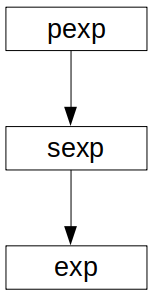
\includegraphics[width=0.15\textwidth]{exp_relation.png}
\caption{The Layer of Expressions in RCIR+}
\label{fig:exp-layer}
\end{figure}

The bottom level ($exp$) contains traditional quantum gates, like \texttt{X}, \texttt{CU}, \texttt{Rz} gates. On top of it, there is a set of operations ($sexp$) that deal with quantum state position swapping. Due to the virtual locations, the position swapping does not really have any effects in the actual physical quantum state locations. Instead, it changes the "view of qubits", which means we change the mapping from virtual state locations to physical locations. The top level ($pexp$) is to switch state space, which means that all operations there enforce certain type of state changes from one form to the other. We will discuss these expressions one by one. 

The syntax of the bottom level ($exp$) is described as follows:

\[
\begin{array}{l}
 exp \;= \texttt{SKIP}\; p \;|\; \texttt{X} \;p\; | \;\texttt{CU} \;p\; exp
        \;| \;\texttt{RZ} \;nat \;p
        \;|\; \texttt{RRZ} \;nat\; p 
\\\qquad
        \;|\; \texttt{SR}\; nat\; var
        \;|\; \texttt{SRR}\; nat\; var
        \;|\; \texttt{HCNOT} \;p\;p
        \;|\; \texttt{Seq} \;exp\; exp
\end{array}
\]

In $exp$, $p$ is a pair of a variable and a natural number. It represents the virtual location of a qubit state, and the application virtual location of a gate. The natural number ($n$, type: \texttt{nat}) appeared in the \texttt{RZ} and \texttt{RRZ} gates represents the rotation angle $2\pi i *\frac{1}{2^n}$ and $2\pi i *(1-\frac{1}{2^n})$, respectively. \texttt{RZ} represents actually the so-called \texttt{Rk} gate \cite{2000quant} in many traditional quantum gate descriptions, and \texttt{RRZ} is to apply an inverse \texttt{Rk} gate, which has the effect of applying the rotation $2\pi i *(1-\frac{1}{2^n})$ on the qubit state. 
\texttt{SR} gate is a special gate that is only used in \texttt{Phi} mode. It is actually a shortcut for a series of \texttt{RZ} gates. 
In \texttt{Phi} space, each qubit forms a suffix relation. In the first qubit in a \texttt{Phi} space, the $i$-th rotation position has to be the same as the $(i - m)$-th position for the $m$ qubit where $m\le i$. We call any of the rotation position across different qubits as linked rotation position. The \texttt{SR} gate is to enforce that every lined rotation position happened in \texttt{Phi} must rotate at the same angle every time. Otherwise, once we apply an inverted QFT after a rotation is applied to a \texttt{Phi} space, the system is not turned back to normal space. \texttt{SRR} is similar to \texttt{SR} but it contains a series of \texttt{RRZ} gates instead of \texttt{RZ} gates. \texttt{HCNOT} gate is essentially a \texttt{CNOT} gate with the restriction that the two positions must all in \texttt{Had} space. We will see examples of using these gates in the next section.

\begin{figure}[h]
\centering
\[\footnotesize
\begin{array}{l}
\begin{array}{llll}
\begin{array}{l}
\texttt{(1)}\;
\AxiomC{$$}
\UnaryInfC{$ \Gamma \vdash \texttt{SKIP}\;p$}
\DisplayProof
\end{array}
&
\begin{array}{l}
\texttt{(2)}\;
\AxiomC{$\Gamma(\texttt{fst}\;p)=\texttt{Nor}$}
\UnaryInfC{$ \Gamma \vdash \texttt{X}\;p$}
\DisplayProof
\end{array}
&
\begin{array}{l}
\texttt{(3)}\;
\AxiomC{$\Gamma(\texttt{fst}\;p)=\texttt{Had}$}
\UnaryInfC{$ \Gamma \vdash \texttt{X}\;p$}
\DisplayProof
\end{array}
&
\begin{array}{l}
\texttt{(4)}\;
\AxiomC{$\Gamma(\texttt{fst}\;p)=\texttt{Nor}\quad
 \Gamma\vdash e $}
\UnaryInfC{$ \Gamma \vdash \texttt{CU}\;p\;e$}
\DisplayProof
\end{array}
\end{array}
\\[2em]
\begin{array}{lll}
\begin{array}{l}
\texttt{(5)}\;
\AxiomC{$\Gamma(\texttt{fst}\;p_1)=\texttt{Had}\quad
 \Gamma(\texttt{fst}\;p_2)=\texttt{Had} $}
\UnaryInfC{$ \Gamma \vdash \texttt{CU}\;p_1\;p_2$}
\DisplayProof
\end{array}
&
\begin{array}{l}
\texttt{(6)}\;
\AxiomC{$\Gamma(\texttt{fst}\;p)=\texttt{Nor} $}
\UnaryInfC{$ \Gamma \vdash \texttt{RZ}\;q\;p$}
\DisplayProof
\end{array}
&
\begin{array}{l}
\texttt{(7)}\;
\AxiomC{$\Gamma(\texttt{fst}\;p)=\texttt{Had} $}
\UnaryInfC{$ \Gamma \vdash \texttt{RZ}\;1\;p$}
\DisplayProof
\end{array}
\end{array}
\\[2em]
\begin{array}{lll}
\begin{array}{l}
\texttt{(8)}\;
\AxiomC{$\Gamma(\texttt{fst}\;p)=\texttt{Nor} $}
\UnaryInfC{$ \Gamma \vdash \texttt{RRZ}\;q\;p$}
\DisplayProof
\end{array}
&
\begin{array}{l}
\texttt{(9)}\;
\AxiomC{$\Gamma(\texttt{fst}\;p)=\texttt{Had} $}
\UnaryInfC{$ \Gamma \vdash \texttt{RRZ}\;1\;p$}
\DisplayProof
\end{array}
&
\begin{array}{l}
\texttt{(10)}\;
\AxiomC{$\Gamma(x)=\texttt{Phi}\;n\quad
m<n $}
\UnaryInfC{$ \Gamma \vdash \texttt{SR}\;m\;x$}
\DisplayProof
\end{array}
\end{array}
\\[2em]
\begin{array}{ll}
\begin{array}{l}
\texttt{(11)}\;
\AxiomC{$\Gamma(x)=\texttt{Phi}\;n\quad
m<n $}
\UnaryInfC{$ \Gamma \vdash \texttt{SRR}\;m\;x$}
\DisplayProof
\end{array}
&
\begin{array}{l}
\texttt{(12)}\;
\AxiomC{$\Gamma \vdash \;e_1\quad \Gamma \vdash \;e_2 $}
\UnaryInfC{$ \Gamma \vdash \;\texttt{Seq}\;e_1\;e_2$}
\DisplayProof
\end{array}
\end{array}
\end{array}
\]
\caption{Well-Typed Definition For Exp}
\label{fig:exp-well-typed}
\end{figure}

The semantics of the expression is basically the same as ones appeared in SQIR. The only difference is that we are dealing with quantum states that are no entanglements. Therefore, the semantic description is more about to define the situation of applying different gates in the three modes of qubit states described above. The only tricky item here is that we have restrictions on the usage of different gates in different state modes. The relation that defines which gate is allowed to run on which mode is described in Fig.~\ref{fig:exp-well-typed}. In the figure, $\Gamma$ is a map from variables to modes. For example, \texttt{X} gates are allowed in the \texttt{Nor} and \texttt{Had} modes, while the control positions of \texttt{CU} gates are only allowed to run on the \texttt{Nor} mode, but the sub-expression of a \texttt{CU} gate can be run in other modes. \texttt{RZ} gate is fully allowed to run on the \texttt{Nor} mode, while if it is run on \texttt{Had}, the rotation angle is only allowed to be \texttt{1}, which means that the gate is a Pauli-Z gate. It is possible to extend the limitation to include \texttt{P} and \texttt{T} gates, but it will require more advanced state representation for \texttt{Had} mode. 
\texttt{SR} and \texttt{SRR} gates are \texttt{Phi} mode specific gates, while the two positions of \texttt{HCNOT} gates must be in the \texttt{Had} mode.

The second level expression ($sexp$) is mainly for swapping state positions. The syntax of $sexp$ is described as follows:

\[
sexp \;= \;\texttt{Lshift}\;x \;|\; \texttt{Rshift}\;x \;|\;\texttt{Rev}\;x 
                 \;|\; \texttt{Exp}\; exp \;|\; \texttt{SSeq} \;sexp\; sexp
\]

The variable $x$ in some expressions represents the virtual locations of a group of qubits. It has the same meaning as the first element of a pair $p$ appeared in $exp$. \texttt{Lshift} is to shift qubit virtual positions one step towards left for all qubits in $x$. If $x$ is allocated to have $n$ qubits, then, after the shift, the relation of the new state function $f'$ and the old one $f$ is: $f'(x,(i+1) \% n) = f(x,i)$ for $i=0,...,n-1$. \texttt{Rshift} is the opposite of \texttt{Lshift}, and the relation between $f'$ and old $f$ is: $f'(x,i) = f(x,(i+1)\%n)$ for $i=0,...,n-1$. \texttt{Rev} (the reverse operation) is to make the qubit positions up-side-down in $x$. Its semantic relation between $f'$ and old $f$ is given as: $f'(x,n-1-i) = f(x,i)$ for $i=0,...,n-1$.

The power of RCIR+ on dealing with these position swapping operations is that the compilations of these operations to SQIR all generate \textbf{zero} gates! During the compilation, instead of generating actually swap gates to do the operations, we actually change the mapping function from virtual qubit locations to its physical locations. For example, if we have a variable $x$ containing \texttt{4} qubits, and we applying a series of operations on it, such as $\texttt{SSeq}\;(\texttt{Lshift}\;x)\;e$. In this expression, $e$ is an expression that is applied to $x$ after the left-shift operation. Before applying the shift, let's assume that the compilation mapping is $\{(x,0) \mapsto 0, (x,1) \mapsto 1, (x,2) \mapsto 2, (x,3) \mapsto 3\}$. Then, after applying the shift, the compilation mapping becomes  $\{(x,3) \mapsto 0, (x,2) \mapsto 1, (x,1) \mapsto 2,(x,3) \mapsto 0\}$. Then, we also pass the mapping to deal with the applications in $e$. 

Since there is no \texttt{CU} gates in the $sexp$ and the top level, this mappings on each step can be generated during the program compilation time. One limitation is that, in RCIR+, one can never write a program with the \texttt{CU} gate on top of an expression containing these shift and reverse operations. We can call our shift/reverse operations as the static shift/reverse operations. If users really want the "dynamic" ones that live inside a \texttt{CU} gate, they can always define \texttt{SWAP} gates by using RCIR+. However, what we found out during the definition of the modulo-multiplication algorithm in RCIR+ is that we don't need to have "dynamic" shift/reserve operations and the static shift/reverse operations in RCIR+ can satisfy any needs in the algorithm. 

The top level expression ($pexp$) is to do another kind of "swapping" operations that swap/shift the qubit state modes, which is orthogonal with respect to the position swapping operations described above. The syntax of $pexp$ is described as follows:

\[
pexp \;=\; \texttt{SExp}\;sexp \;|\; \texttt{QFT} \;x \;| \;\texttt{RQFT}\; x
               \;|\; \texttt{H}\; x \;|\; \texttt{FSeq}\;pexp\;pexp
\]

\texttt{QFT} is to allow a quantum fourier transform (QFT) to all qubits in $x$, \texttt{RQFT} is the inverse QFT operation. \texttt{H} is a Hadamard gate. In the $sexp$ level, the types are actually not important since every shift/reverse operation can be applied in any mode. The types re-appear to be important in the $pexp$ level. The gates that live in this level actually shift the qubit state modes from one to the other. 

\begin{figure}[h]
\centering
\[\footnotesize
\begin{array}{l}
\begin{array}{ll}
\begin{array}{l}
\texttt{(13)}\;
\AxiomC{$\Gamma \vdash e$}
\UnaryInfC{$ (\Sigma,\Gamma) \vdash \texttt{SExp}\;e \triangleright \Gamma$}
\DisplayProof
\end{array}
&
\begin{array}{l}
\texttt{(14)}\;
\AxiomC{$\Gamma(x)=\texttt{Nor}\quad \Sigma(x)=n$}
\UnaryInfC{$ (\Sigma,\Gamma) \vdash \texttt{QFT}\;x\triangleright \Gamma[x\mapsto \texttt{Phi}\;n]$}
\DisplayProof
\end{array}
\end{array}
\\[2em]
\begin{array}{ll}
\begin{array}{l}
\texttt{(15)}\;
\AxiomC{$\Gamma(x)=\texttt{Phi}\;n$}
\UnaryInfC{$ (\Sigma,\Gamma) \vdash \texttt{RQFT}\;x\triangleright \Gamma[x\mapsto \texttt{Nor}]$}
\DisplayProof
\end{array}
&
\begin{array}{l}
\texttt{(16)}\;
\AxiomC{$\Gamma(x)=\texttt{Nor}\quad
 \Gamma\vdash e $}
\UnaryInfC{$ (\Sigma,\Gamma) \vdash \texttt{H}\;x\triangleright \Gamma[x\mapsto \texttt{Had}]$}
\DisplayProof
\end{array}
\end{array}
\\[2em]
\begin{array}{ll}
\begin{array}{l}
\texttt{(17)}\;
\AxiomC{$\Gamma(x)=\texttt{Had}$}
\UnaryInfC{$ (\Sigma,\Gamma) \vdash \texttt{H}\;x\triangleright \Gamma[x\mapsto \texttt{Nor}]$}
\DisplayProof
\end{array}
&
\begin{array}{l}
\texttt{(18)}\;
\AxiomC{$(\Sigma,\Gamma)\vdash e_1\triangleright \Gamma'
\quad(\Sigma,\Gamma')\vdash e_2\triangleright \Gamma'' $}
\UnaryInfC{$ (\Sigma,\Gamma) \vdash \texttt{FSeq}\;e_1\;e_2\triangleright \Gamma''$}
\DisplayProof
\end{array}
\end{array}
\end{array}
\]
\caption{Well-Typed Definition For PEXP}
\label{fig:pexp-well-typed}
\end{figure}

The well-typed definition for $pexp$ is listed in Fig.~\ref{fig:pexp-well-typed}. $\Sigma$ is an invariant map that records the number of qubits for each variable in the system. 
\texttt{QFT} can switch a state in the \texttt{Nor} mode to \texttt{Phi}, while \texttt{RQFT} can switch a state from \texttt{Phi} back to \texttt{Nor}. \texttt{H} gate switches the mode from \texttt{Nor} to \texttt{Had}, and switch a state in \texttt{Had} back to \texttt{Nor}.
The semantics of the $pexp$ gates has no essential difference from the same gates defined in SQIR. The only difference is that the gates are dealing with different qubit state representations than the ones in SQIR, and they also need to take care of mode switching.

\section{Example Quantum Circuits}
\label{sec:example}

In this section, we discuss the utility of RCIR+. As we mentioned above, we plan to utilize RCIR+ to analyze quantum circuits. The analysis means that doing property proofs, simulations, and random testing on quantum circuits. 
Here, we provide some example circuits that RCIR+ is capable of analyzing.

A trivial example of using RCIR+ is the ripple-carry adder \cite{ripple-carry}, since the gates used in the adder are essentially \texttt{X}, \texttt{CNOT}, and \texttt{CCX} gates, which are gates that can be analyzed in the \texttt{Nor} mode in RCIR+. 
A good example of using RCIR+ is probably the QFT-based arithmetic circuits. 

\begin{figure}[h]
\centering
     \begin{subfigure}[b]{0.6\textwidth}
         \centering
         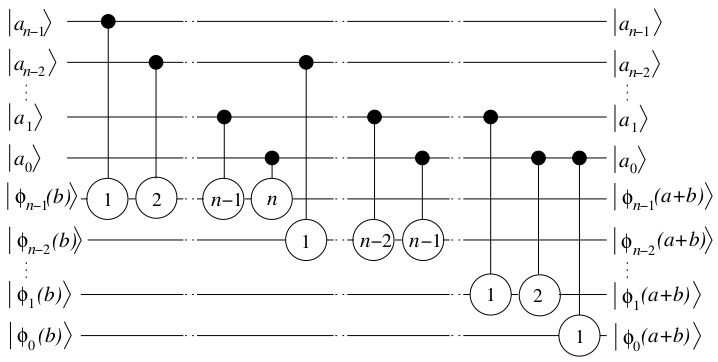
\includegraphics[width=1\textwidth]{qft-addition.png}
         \caption{QFT-based Addition Circuit}
         \label{fig:addition}
     \end{subfigure}%
     ~
     \begin{subfigure}[b]{0.6\textwidth}
         \centering
         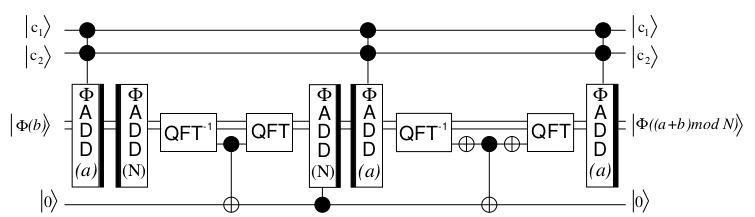
\includegraphics[width=1\textwidth]{qft-mod.png}
         \caption{QFT-based Modulo Multiplier Circuit}
         \label{fig:mod}
     \end{subfigure}

\caption{QFT-based Arithmetic Circuits}
\label{fig:qft-circuit}
\end{figure}

In Fig.~\ref{fig:qft-circuit}, we show the QFT-based addition circuit and a QFT-based modulo multiplier circuit. 
In Fig.~\ref{fig:addition}, the QFT-based addition circuit is assumed to have the input qubits for variable $b$ in the \texttt{Phi} mode, while qubits in variable $a$ are in the \texttt{Nor} mode.
To add the number $a$, which is represented as a binary Boolean values, to the $b$ value, it uses \texttt{CU} gates on variable $a$ qubits, and \texttt{RZ} gates for $b$. In RCIR+, we require gates in the \texttt{Phi} mode to only use \texttt{SR} and \texttt{SRR} gates. By exterminating the circuit carefully, we found that this is actually the case. For every qubit position $i$ in $a$, it touches only the $i$ rotation position in the rotation angle in each qubit of $b$. For example, the second $n-2$ qubit in $a$ rotates $\texttt{RZ}\;1$ in the $n-2$ qubit in $b$, and $\texttt{RZ}\;2$ in the $n-3$ qubit in $b$, and so on. We can conclude that an $n-i$ qubit in $a$ has \texttt{CU}-\texttt{RZ} gates on the $n-m$ qubit in $b$ where $m<i$, and the angle rotated in the $n-m$ qubit is $\texttt{RZ};(i-m+1)$. Hence, the \texttt{RZ} gates for each qubit in $a$ forms a \texttt{SR} gate in RCIR+. 
Fig.~\ref{fig:mod} show how to use mode transformation in RCIR+. We assume that the input for $b$ for the circuit is in the \texttt{Phi} mode, the two QFT-based addition circuits in the left can be done in the \texttt{Phi} mode, and the \texttt{RQFT} gate turns the mode of $b$ back to \texttt{Nor}, then it allows the \texttt{CNOT} gate (\texttt{CU} plus \texttt{X} gates) after \texttt{RQFT} is valid to run in the \texttt{Nor} mode. Then, the \texttt{QFT} gate turns $b$ back to \texttt{Phi}, and some other QFT-based addition operations can be applied on qubits in $b$. 

\begin{figure}[h]
\centering
         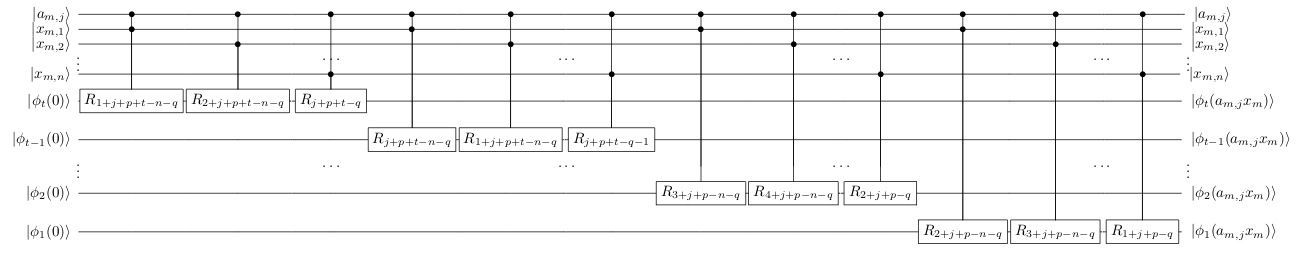
\includegraphics[width=\textwidth]{controlled-weight-sum.png}
\caption{QFT-based Controlled Weighted Sum Circuit}
\label{fig:qft-contol-circuit}
\end{figure}

Basically, all QFT-based arithmetic operations are analyzable by only using \texttt{SR} and \texttt{SRR} gates for \texttt{Phi}-mode qubits (obviously, we need other gates for qubits in the \texttt{Nor} mode). An example in the controlled weighted sum circuit in Fig.~\ref{fig:qft-contol-circuit}, which has the formula: $\Sigma^{2^n}_{m=1}a_m x_m$.

\begin{figure}[h]
\centering
     \begin{subfigure}[b]{0.6\textwidth}
         \centering
         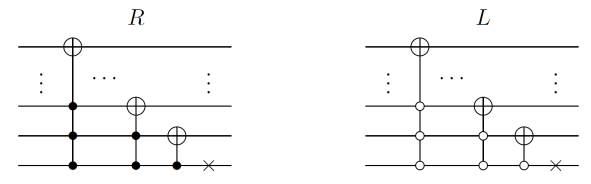
\includegraphics[width=1\textwidth]{lr-circuit.png}
         \caption{Circuits for L and R}
         \label{fig:lr-graph}
     \end{subfigure}

     \begin{subfigure}[b]{0.3\textwidth}
         \centering
         \includegraphics[width=1\textwidth]{circle-8-graph.png}
         \caption{Circle Graph (N = 8)}
         \label{fig:circle}
     \end{subfigure}%
     ~
     \begin{subfigure}[b]{0.7\textwidth}
         \centering
         \includegraphics[width=1\textwidth]{whole-quantum-walk.png}
         \caption{Full Circuit For Circle Graph Quantum Walk Oracle}
         \label{fig:quantum-walk-circle}
     \end{subfigure}

\caption{Quantum Walk Oracle Circuit}
\label{fig:circle-circuit}
\end{figure}

Another example circuit that can be analyzed is the oracle circuits in quantum walk in Fig.~\ref{fig:circle-circuit}. 
Most gates in the circuit are run in the \texttt{Nor} mode, and they can be analyzed by RCIR+. The only possible problem is the controlled-Z gate (\texttt{CZ}, listed as controlled $\pi$ in the Fig~\ref{fig:quantum-walk-circle}) surrounded by two \texttt{H} gates. In RCIR+, \texttt{CZ} gates are essentially \texttt{CU} gates and a $\texttt{RZ}$ gate with a rotation of angle $\pi$, and the \texttt{CU} gates are applied on qubits in \texttt{Nor}, as well as the \texttt{RZ} gate is applied on a qubit in the \texttt{Had} mode.
In Fig.~\ref{fig:quantum-walk-circle}, it seems that the \texttt{CZ} gate is applied on a controlled qubit in \texttt{Had} and all other qubits to be in \texttt{Nor}. What we find out is that these two \texttt{CZ} gate applications have the same effect. Any vector that is applied by a \texttt{CZ} gate where all controlled qubits are in \texttt{Nor} and the \texttt{RZ} applied qubit in the \texttt{Had} mode has the same effect as the one that is applied by a \texttt{CZ} gate where any one of the controlled qubit is in \texttt{Had} and all other qubits are in \texttt{Had}. This is why we are able to use RCIR+ to analyze the quantum walk oracle circuit in Fig.~\ref{fig:circle-circuit}.

\begin{figure}[h]
\centering
     \begin{subfigure}[h]{0.25\textwidth}
         \centering
         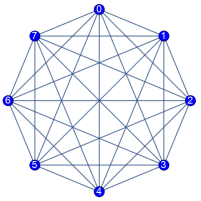
\includegraphics[width=1\textwidth]{k-graph.png}
     \end{subfigure}%
     ~
     \begin{subfigure}[h]{0.5\textwidth}
         \centering
         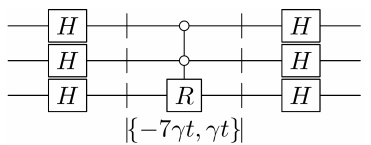
\includegraphics[width=1\textwidth]{tim-evolve-k-graph.png}
     \end{subfigure}
\caption{Quantum Walk Time-evolution Operator for $K_8$ Graph}
\label{fig:quantum-walk-time-evol}
\end{figure}

Unfortunately, not all quantum walk algorithm components are analyzable in RCIR+ with the qubit inputs to be in the \texttt{Nor} mode. 
Fig.~\ref{fig:quantum-walk-time-evol} shows a time-evolution operator in quantum walk for a $K_8$ graph.
This circuit is not analyzable in RCIR+ if the input qubits are in \texttt{Nor}.
To analyze this circuit in RCIR+, we first investigate an important theorem in dealing with quantum circuits in Observation~\ref{basic-state-thm}. 

\begin{observation}
\label{basic-state-thm}
\rm
If a quantum algorithm property is correct for all basis-vector inputs, the property can be extended for general quantum inputs.
\end{observation}

This Observation is a direct corollary from a theorem that is proved in the VOQC project \cite{10.1145/3434318}, where if two matrices produce the same output when they are multiplied by any basis-vector (a vector with $1$ in one row and $0$ in any other rows), then the two matrices are the same. An application of a quantum algorithm on an input is essentially to do a matrix multiplication on vectors as the input. The theorem tells us that if two algorithms are the same, then we only need to see if all basis-vectors as input for the two algorithms are the same. In contrast, if two quantum algorithms are tested to be the same under all basis-vectors, then we are not able to distinguish them by any input. In other word, if an algorithm property is correct in one algorithm $\sigma$, and there is another algorithm $\delta$ that is tested the same as $\sigma$ with all basis-vector inputs, then the property is also held in the algorithm $\delta$, because essentially algorithm properties are based on the input and output of algorithms. 

On the other hand, since all quantum algorithms are essentially matrix-vector multiplications, and any vectors can be viewed as a sum of scale multiplications of several basis vectors, if a property is held for all basis-vectors for an algorithm, the output behaviors of the property is calculable for arbitrary input vectors. 
This Observation can be extended to other forms of "basis" inputs for a quantum algorithms. Essentially, a basis-vector is a Kronecker product of qubits $|0>$ and $|1>$. One can produce a proportional relation between qubits $|+>$ ($\frac{1}{\sqrt{2}}(|0>+|1>)$) and $|->$ ($\frac{1}{\sqrt{2}}(|0>-|1>)$) are qubits $|0>$ and $|1>$. For example, $|0>\propto |+> + |->$. Hence, if a algorithm property is preserved for any Kronecker product of arbitrary $|+>$ and $|->$ (actually, we just need to analyze an arbitrary Kronecker product of exactly one $|->$ and many $|+>$), for arbitrary input qubits, the effects of the property is also calculable. 
For example, in dealing with the time-evolution operator in Fig.~\ref{fig:quantum-walk-time-evol}, if we assume that the input is an Kronecker product of $|+>$ and $|->$, then the inputs are in the \texttt{Had} mode, with the application of \texttt{H} gates, we can then analyze the effects of the \texttt{CU}-\texttt{RZ} gate in the middle. The quantum states to analyze in this format is a lot simpler than the ones if we assume that the input is with qubits $|0>$ and $|1>$. Additionally, if we keep the input as Kronecker products of $|+>$ and $|->$, in every computation step of the time-evolution operator, the quantum state is not entangled, which means that we can separately analyze every single qubit individually during the process. The direct consequence of analyzing the operator by using $|+>$ and $|->$ qubits is that we are able to design a traditional random testing algorithms to capture the behaviors for the time-evolution operator. We can then design the random testing kit in RCIR+ to have both inputs of Kronecker products of $|0>$ and $|1>$ (the \texttt{Nor} mode) and Kronecker products of $|+>$ and $|->$ (the \texttt{Had} mode) , so the random testing kit in RCIR+ now is able to show behaviors of more quantum algorithms. 

\begin{figure}[h]
\centering
         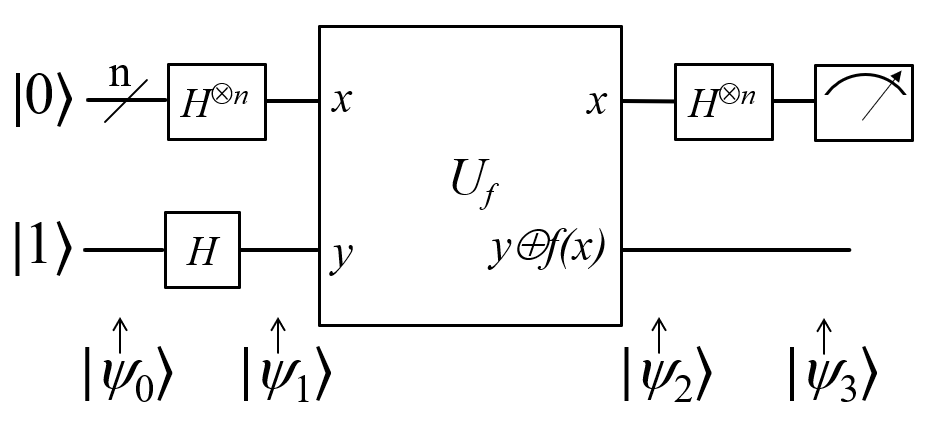
\includegraphics[width=0.5\textwidth]{deutsch-jozsa.png}
\caption{Deutsch-Jozsa Circuit}
\label{fig:Deutsch–Jozsa}
\end{figure}

A usage of the $|+>$/$|->$ qubit inputs is the analysis of the Deutsch–Jozsa algorithm (Fig.~\ref{fig:Deutsch–Jozsa}). By using the \texttt{Had} mode input, we are able to show the behaviors of step computations in this algorithm, and then for each step, we can produce the output behaviors of the algorithm with \texttt{Nor} mode input with a proper calculation. 

\section{An Example Usage of RCIR+: QSSA}
\label{sec:qssa}

One of the example usage of RCIR+ is the compilation of a high level SSA-formed (static single assignment formed) language with only arithmetic operations, such as math addition, subtraction, and multiplication, etc.

We first list the grammar of QSSA below:

\[
\begin{array}{l}
 fact \;= \texttt{Var}\; var \;|\; \texttt{Num} \;nat
\qquad
flag \;=\texttt{QFTA}\;|\;\texttt{Classic}
\qquad
bty\;=\texttt{Nat}\;|\;\texttt{Float}
\\[0.5em]
iexp \;=\texttt{plus}\;flag\;fact\;fact\;|\;\texttt{minus}\;flag\;fact\;fact\;|\;\texttt{mult}\;flag\;fact\;fact
\\\quad\;|\;\texttt{div}\;flag\;fact\;fact\;|\;\texttt{mod}\;flag\;fact\;fact\;|\;\texttt{load}\;var
\\[0.5em]
cexp \;=\texttt{clt}\;flag\;fact\;fact\;|\;\texttt{ceq}\;flag\;fact\;fact
\\[0.5em]
qexp\;=\texttt{inst}\;var\;nat\;bty\;iexp\;|\;\texttt{add}\;flag\;fact\;fact\;|\;\texttt{sub}\;flag\;fact\;fact
\\\quad\;|\;\texttt{times}\;flag\;fact\;fact
\;|\;\texttt{call}\;fvar
\;|\;\texttt{if}\;cexp\;qexp\;qexp
\;|\;\texttt{while}\;cexp\;qexp
\\\quad
\;|\;\texttt{ret}\;(list\;(var * var))
\;|\;\texttt{seq}\;qexp\;qexp
\\[0.5em]
fun\;=(fvar * qexp)
\qquad
prog\;=(nat * nat * nat * list\;(var * nat) * list\;fun)
\end{array}
\]

In QSSA, each variable is either a value representing a natural number (\texttt{Nat}) of a floating pointer number (\texttt{Float}). In addition, a variable can be either a global variable or a local variable. The expression \texttt{load} loads the value in a global variable to a local variable. The instruction \texttt{ret} returns a list of pairs of variables when a function is returned. In each pair $(x,u)$, $x$ must be a global variable and $u$ must be a local variable. The semantic meaning of \texttt{ret} for each pair $(x,u)$ is that $x:=u\oplus x$. From $iexp$, except \texttt{load}, all other expressions in QSSA are arithmetic operations. The $flag$ in each expression is either \texttt{QFTA} or \texttt{Classic}, meaning that the expression is computed using a QFT-based circuit and a classical circuit, respectively. $qexp$ represents instructions in a function. The basic instruction is $\texttt{inst}\;x\;n\;ty\;e$, where $x$ is the target variable to store the computation result, $n$ represents the number of bits in variable $x$, $ty$ defines if the value is a floating-point value or a natural number, and $e$ is an expression ($iexp$). All basic instructions $\texttt{inst}$ are required to be in SSA-format in a function, meaning that an variable $x$ in an \texttt{inst} can be assigned only once. For any \texttt{inst} having the form $x:=y\;\texttt{op}\;z$, it is corresponding to a reversible computation having the form as $[y][z][0]\rightarrow[y][z][x]$, where $x$ is the computation result of $y\;\texttt{op}\;z$.

In QSSA, we have a branching operation \texttt{if} and a loop operation \texttt{while}. Their Boolean guards are $cexp$ expressions. We currently allow users to compare if one value is smaller than the other one ($\texttt{clt}$), or if they are equal (\texttt{ceq}). 
In the body of a \texttt{while} loop in QSSA, we require that there is no basic instructions (\texttt{inst}). Instead, we provide three different operations for users in a loop body: \texttt{add}, \texttt{sub}, and \texttt{times}, with other kinds of instructions like \texttt{call}, \texttt{if}, \texttt{while}, \texttt{ret}, and \texttt{seq}. \texttt{add}, \texttt{sub}, and \texttt{times} represents math addition, subtraction, and multiplication, respectively. The difference between them and the ones in \texttt{inst} is the reversible computation formation. These three operations have the form: $[x][y]\rightarrow[x][y\;\texttt{op}\;x]$; so \texttt{add} can be better understood as "adding to", and \texttt{sub} is more like "subtracting from". We have the separation because of the efficiency concerns. Eventually, all variables in a QSSA function is mapped to an array of qubits. If we need to create a variable every time when a re-enter a loop body, this might not be feasible in the current status of a quantum circuit. Instead, most users might be interested in creating a variable before entering a loop, and updating the value in the variable when re-entering the loop. 
For each function ($fun$), there is also two global setting numbers that are related to the execution of a loop. The first number defines the stack size of a function, and the second number defines the maximum number of steps for executing a loop. The problem of having a loop in a quantum circuit is the loop Boolean guard. When executing a loop, every Boolean guard needs to be stored in a qubit, and for every step of computation, once a qubit is used for a Boolean guard, it cannot be re-used in the further step of loop-evaluation before the loop computation is finished. Hence, the compiler needs to know a place to swap clean ancillary qubits for storing a Boolean guard value.This is the so-called stack for a function, and the stack size for each function is pre-determined. In addition, for each loop execution, the maximum number of steps is also pre-determined, due to the fact that our compiler needs to expand the loop code before executing the loop operation.

In QSSA, function calls have no arguments at this point, and it is also not recursive. The usage of a function is to provide a automatic inverse circuit. For a function having the form: $f()\{e;\texttt{ret}\; l\}$, it is actually to execute the following: $e;\texttt{ret}\; l;\texttt{inv}\;e$. We first evaluate the function body $e$, and then the return instruction copies all local variables to global variables, and then we do an inverse of the function body $e$ (\texttt{inv}). 

Now, we discuss some about the compilation and type system of QSSA. Each variable in QSSA is having a type that is represented as a tuple of two different type fragments as: 

\[
\begin{array}{l}
bty\;=\texttt{Nat}\;|\;\texttt{Float}
\quad
aty\;=\texttt{C}\;nat\;|\;\texttt{Q}\;nat
\quad
type\;=(aty * bty)
\\[0.5em]
\end{array}
\]

Other than the \texttt{bty} fragment to classify if a variable representing a float or a natural number, the \texttt{aty} fragment checks if the value of a variable is "statically" determinable or "dynamically" determinable. 
The meaning of "statical"/"dynamical" determination is different from the version used in a classical compiler field. Here, we refer to statically determinable variable as its value is commutable without using quantum circuits, while dynamically determinable variable must hand to a quantum circuit to compute its value. The logic behinds this classification is that any effective computation that is compatible in a classical computer is a lot "cheaper" than doing the computation in a quantum machine.
The QSSA type system and compiler aggressively checks every line of code in a function and finds statically determinable variables as much as possible and per-compute all values for all statically determinable variables, and then we generate quantum circuits for only dynamical determinable variables.

A key observation of doing the compilation from QSSA to RCIR+ is that every operation in QSSA is a computation starting at a \texttt{Nor} mode and also ends at a \texttt{Nor} mode. If we think of the instruction in QSSA in terms of a compiled circuit in RCIR+, we find that the input for every operation is basically a series of qubits $|0>$ and $|1>$, and the output for every operation is also a series of $|0>$ and $|1>$. No matter the middle circuit is a QFT-based or a classical circuit, if the starting mode is \texttt{Nor}, then the ending mode is also \texttt{Nor}. This observation ease the compilation proofs from QSSA to RCIR+, and it also enables us to have a rich language representation.

One final thing worth noting is that QSSA is an example of using RCIR+. RCIR+ might enables more operations than the set of QSSA instructions listed here, such as the graph oracles and time evolving operators in quantum walk algorithms. For some enhanced quantum oracles or algorithm components, users might want to write their own effective circuit implementation in RCIR+. The RCIR+ random testing kit provides a way for helping users to validate and debug their large circuit implementations without going through the "pain" of proving the correctness of a compiler. 

\section{Evaluation and Future Study}
\label{sec:eval}
 
Currently, I have finished implementing the type system and semantics for RCIR+. I have already proved the correctness of compilation from RCIR+ to SQIR for $exp$ and $sexp$. I also the classical and QFT-based modulo multiplier on RCIR+, as well as the correctness proof for the classical modulo multiplier. There are several takeaways here. 

First, RCIR+ solves the problem of "can". By using RCIR+, we are able to define the classical and QFT-based adders and other oracle algorithms in a \textbf{single} framework. I also plan to define Grover's algorithm, as well as quantum walk algorithms in RCIR+. 
Second, RCIR+ also helps reduce the compilation gates. In dealing with the classical modulo multiplier, we are able to reduce 60\% of the
gates when we compile the circuit to SQIR. This is mainly because the fact that we don't need to do any static shift/reverse operations as well as reduce many swap operations. 
Third, RCIR+ helps the problem of "simplification". In defining the modes and restricting when a gate can be applied, we are able to avoid qubits having entanglements. This will certainly help simplifying the analysis of many quantum algorithms, especially oracle algorithm, that do not rely on entanglements. 
In addition, we can simplify the design of an RCIR+ simulator because the three different modes of qubit states that are based on natural numbers can improve the performance. 

For future study, I plan to define the sine/cosine functions based on the cordic method that relies on addition and shift operations, as well as many quantum oracles and components in quantum walk. Since I have finished the design for classical and QFT-based modulo multipliers, these automatically give us the addition, subtraction, and multiplication operations. These can be the basis of the compilation from QSSA to RCIR+. I can imagine the compilation will be easy to do since we have all separated components. Please feel free to talk to me and I need cooperation. 





%%Acknowledgments
\begin{acks}                            %% acks environment is optional
                                        %% contents suppressed with 'anonymous'
  %% Commands \grantsponsor{<sponsorID>}{<name>}{<url>} and
  %% \grantnum[<url>]{<sponsorID>}{<number>} should be used to
  %% acknowledge financial support and will be used by metadata
  %% extraction tools.
  % This material is based upon work supported by the
  % \grantsponsor{GS100000001}{National Science
  %   Foundation}{http://dx.doi.org/10.13039/100000001} under Grant
  % No.~\grantnum{GS100000001}{nnnnnnn} and Grant
  % No.~\grantnum{GS100000001}{mmmmmmm}.  Any opinions, findings, and
  % conclusions or recommendations expressed in this material are those
  % of the author and do not necessarily reflect the views of the
  % National Science Foundation.
We thank Leonidas Lampropoulos for helping us with effective use of
QuickChick, and Aaron Green and Robert Rand for helpful comments and contributions
during the development of this work. This material is based upon work supported
by the U.S. Department of 
Energy, Office of Science, Office of Advanced Scientific Computing
Research, Quantum Testbed Pathfinder Program under Award Number
DE-SC0019040, and the Air Force Office of Scientific Research under Grant No.
FA95502110051.
\end{acks}


%% Bibliography
\bibliography{reference}
\newpage
\section{\oqasm: An Assembly Language for Quantum Oracles}
\label{sec:vqir}

\begin{figure}[t]
{\small
  \begin{lstlisting}[numbers=left,language=C++,xleftmargin=4 mm]
method Shor ( a : int, N : int, n : int, m : int, x : Q[n], y : Q[n] )
 requires (n > 0)
 requires (1 < a < N)
 requires (N < 2^(n-1))
 requires (N^2 < 2^m <= 2 * N^2)
 requires (gcd(a, N) == 1)
 requires ( type(x) = Tensor n (Nor 0))
 requires ( type(y) = Tensor n (Nor 0))
 ensures (gcd(N, r) == 1)
 ensures (p.pos >= 4 / (PI ^ 2))
{
  x *= H ;
  y *= cl(y+1); //cl can be omitted.
  for (int i = 0; i < n; x[i]; i ++)
    invariant (0 <= i <= n)
    invariant (saturation(x[0..i]))
    invariant (type(y,x[0..i]) = Tensor n (ch (2^i) {k | j baseof x[0..i] && k = (a^j mod N,j)}))
    //psum(k=b,M,p(k),b(k)) = sum_{k=b}^M p(k)*b(k)
    invariant ((y,x[0..i]) == psum(k=0,2^i,1,(a^k mod N,k))) 
  {
    y *= cl(a^(2^i) * y mod N);
  }

 M z := measure(y);//partial measurement, actually measure(y,r) r is the period
 x *= RQFT;
 M p := measure(x); //p.pos and p.base
 var r := post_period(m,p.base) // exists t. 2^m * t / r = p.base
}
  \end{lstlisting}
}
\caption{Shor's Algorithm in Q-Dafny}
\label{fig:shorexample}
\end{figure}

We designed \oqasm to be able to express efficient quantum
oracles that can be easily tested and, if desired, proved
correct.
\oqasm operations leverage both the standard
computational basis and an alternative basis connected by the quantum
Fourier transform (QFT). 
\oqasm's type system tracks the bases of variables in
\oqasm programs, forbidding operations that would introduce
entanglement. \oqasm states are therefore efficiently
represented, so programs can be effectively tested and are simpler to
verify and analyze. In addition, \oqasm uses \emph{virtual qubits}
to support \emph{position shifting operations}, which support
arithmetic operations without introducing extra gates during
translation. All of these features are novel to quantum assembly
languages. 

This section presents \oqasm states and the language's syntax,
semantics, typing, and soundness results.  As a running example, we use the QFT
adder~\cite{qft-adder} shown in \Cref{fig:circuit-example}. The Coq
function \coqe{rz_adder} generates an \oqasm program that adds two
natural numbers \coqe{a} and \coqe{b}, each of length \coqe{n} qubits.

\begin{figure*}[t]
  \centering
  \begin{tabular}{c @{\quad} c}
  \begin{minipage}[b]{.55\textwidth}
  % 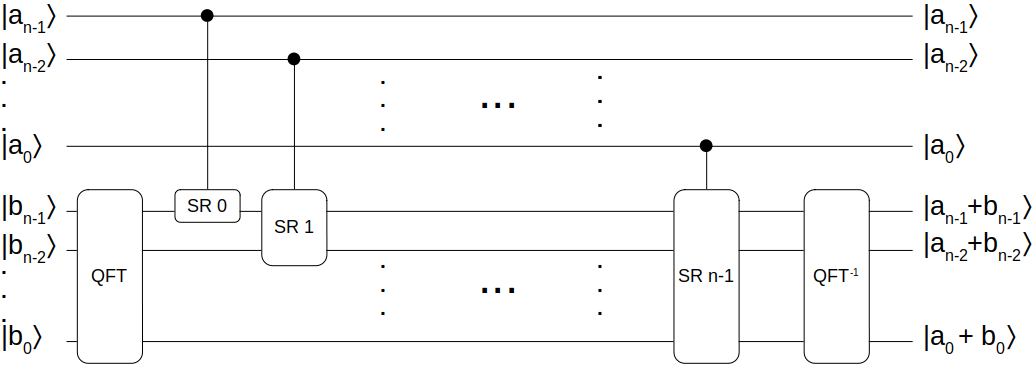
\includegraphics[width=1\textwidth]{qft-adder.png}
    \Small
    \Qcircuit @C=0.5em @R=0.75em {
      \lstick{\ket{a_{n-1}}} & \qw & \ctrl{5} & \qw & \qw & \qw & \qw & \qw & \qw & \qw & \rstick{\ket{a_{n-1}}} \\
      \lstick{\ket{a_{n-2}}} & \qw & \qw & \ctrl{4} & \qw & \qw & \qw & \qw & \qw & \qw & \rstick{\ket{a_{n-2}}}\\
      \lstick{\vdots} & & & & & & & & & & \rstick{\vdots} \\
      \lstick{} & & & & & & & & & & \\
      \lstick{\ket{a_0}} & \qw & \qw & \qw & \qw & \qw & \qw & \ctrl{1} & \qw & \qw & \rstick{\ket{a_0}} \\
      \lstick{\ket{b_{n-1}}} & \multigate{5}{\texttt{QFT}} & \gate{\texttt{SR 0}} & \multigate{3}{\texttt{SR 1}} & \qw & \qw & \qw & \multigate{5}{\texttt{SR (n-1)}} & \multigate{5}{\texttt{QFT}^{-1}} & \qw & \rstick{\ket{a_{n-1} + b_{n-1}}} \\
      \lstick{} & & & & & \dots & & & & \\
      \lstick{\ket{b_{n-2}}} & \ghost{\texttt{QFT}} & \qw  &  \ghost{\texttt{SR 1}} & \qw & \qw & \qw & \ghost{\texttt{SR (n-1)}} & \ghost{\texttt{QFT}^{-1}} & \qw & \rstick{\ket{a_{n-2} + b_{n-2}}} \\
      \lstick{\vdots} & & & & & & & & & & \rstick{\vdots} \\
      \lstick{} & & & & & & & & & & \\
      \lstick{\ket{b_0}} & \ghost{\texttt{QFT}} & \qw & \qw & \qw & \qw & \qw & \ghost{\texttt{SR (n-1)}} & \ghost{\texttt{QFT}^{-1}}  & \qw & \rstick{\ket{a_0 + b_0}} 
      }
  \subcaption{Quantum circuit}
  \end{minipage} &
  \begin{minipage}[b]{.35\textwidth}
  \begin{coq}
  Fixpoint rz_adder' (a b:var) (n:nat) 
    := match n with 
       | 0 => ID (a,0)
       | S m => CU (a,m) (SR m b); 
                rz_adder' a b m
       end.
  Definition rz_adder (a b:var) (n:nat) 
    := Rev a ; Rev b ; $\texttt{QFT}$ b ;
       rz_adder' a b n;
       $\texttt{QFT}^{-1}$ b; Rev b ; Rev a.
  \end{coq}
  \subcaption{\oqasm metaprogram (in Coq)}
  \end{minipage}
  \end{tabular}
  \vspace{-0.5em}
  \caption{Example \oqasm program: QFT-based adder}
  \label{fig:circuit-example}
  \end{figure*}

\subsection{\oqasm States} \label{sec:pqasm-states}

\begin{figure}[t]
  \small
  \[\hspace*{-0.5em}
\begin{array}{l>{$} p{1.2cm} <{$} c l}
      \text{Bit} & b & ::= & 0 \mid 1 \\
      \text{Natural number} & n & \in & \mathbb{N} \\
      \text{Real} & r & \in & \mathbb{R}\\
      \text{Phase} & \alpha(r) & ::= & e^{2\pi i r} \\
      \text{Basis} & \tau & ::= & \texttt{Nor} \mid \texttt{Phi}\;n \\
      \text{Unphased qubit} & \overline{q} & ::= & \ket{b} ~~\mid~~ \qket{r} \\
      \text{Qubit} & q & ::= &\alpha(r) \overline{q}\\
      \text{State (length $d$)} & \varphi & ::= & q_1 \otimes q_2 \otimes \cdots \otimes q_d
    \end{array}
  \]
  \caption{\oqasm state syntax}
  \label{fig:vqir-state}
\end{figure}

An \oqasm program state is represented according to the grammar in
\Cref{fig:vqir-state}. A state $\varphi$ of $d$ qubits is 
a length-$d$ tuple of qubit values $q$; the state models the tensor
product of those values. This means that the size of $\varphi$ is
$O(d)$ where $d$ is the number of qubits. A $d$-qubit state in a
language like \sqir is represented as a length $2^d$ vector of complex
numbers, which is $O(2^d)$ in the number of qubits.  Our linear state
representation is possible because applying any well-typed \oqasm
program on any well-formed \oqasm state never causes qubits to be
entangled.

A qubit value $q$ has one of two forms $\overline{q}$, scaled by a
global phase $\alpha(r)$. The two forms depend on the \emph{basis}
$\tau$ that the qubit is in---it could be either \texttt{Nor} or \texttt{Phi}. A \texttt{Nor} qubit has form
$\ket{b}$ (where $b \in \{ 0, 1 \}$), which is a
computational basis value. 
A \texttt{Phi} qubit has form $\qket{r} = \frac{1}{\sqrt{2}}(\ket{0}+\alpha(r)\ket{1})$, which is a value of the (A)QFT basis.
The number $n$ in \texttt{Phi}$\;n$ indicates the precision of the state $\varphi$.
As shown by~\citet{qft-adder}, arithmetic on the computational basis can sometimes be more efficiently carried out on the QFT basis, which leads to the use of quantum operations (like QFT) when implementing circuits with classical input/output behavior.
 
\subsection{\oqasm Syntax, Typing, and Semantics}\label{sec:oqasm-syn}

\liyi{add RZ gate back}

\begin{figure}[t]
\begin{minipage}[t]{0.5\textwidth}
{\small \centering

  $ \hspace*{-0.8em}
\begin{array}{llcl}
      \text{Position} & p & ::= & (x,n) \qquad   \text{Nat. Num}~n
                                  \qquad   \text{Variable}~x\\
      \text{Instruction} & \instr & ::= & \iskip{p} \mid \inot{p}
                                          \mid \irz[\lbrack -1 \rbrack]{n}{p} \mid \iseq{\instr}{\instr}\\
                & & \mid &  \isr[\lbrack -1 \rbrack]{n}{x} \mid \iqft[\lbrack -1 \rbrack]{n}{x} \mid \ictrl{p}{\instr}  \\
                      & & \mid & \ilshift{x} \mid \irshift{x} \mid \irev{x} 
    \end{array}
  $
}
  \caption{\oqasm syntax. For an operator \texttt{OP}, $\texttt{OP}^{\lbrack -1 \rbrack}$ indicates that the operator has a built-in inverse available.}
  \label{fig:vqir}
\end{minipage}
\hfill
\begin{minipage}[t]{0.45\textwidth}
\centering
\begin{tabular}{c@{$\quad=\quad$}c}
  \begin{minipage}{0.3\textwidth}
  \Small
%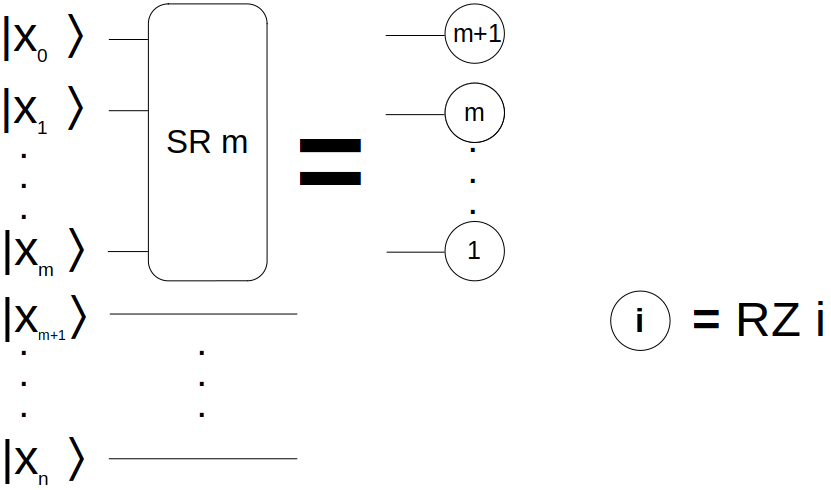
\includegraphics[width=0.3\textwidth]{sr-meaning.png}
  \Qcircuit @C=0.5em @R=0.5em {
    \lstick{} & \qw     & \multigate{4}{\texttt{SR m}} & \qw & \qw \\
    \lstick{} & \qw     & \ghost{\texttt{SR m}}           & \qw & \qw \\
    \lstick{} & \vdots & & \vdots & \\
    \lstick{} & & & & \\
    \lstick{} & \qw     & \ghost{\texttt{SR m}}           & \qw  & \qw
    }
  \end{minipage} & 
  \begin{minipage}{0.3\textwidth}
  \Small
  \Qcircuit @C=0.5em @R=0.5em {
    \lstick{} & \qw     & \gate{\texttt{RZ (m+1)}} & \qw & \qw \\
    \lstick{} & \qw     & \gate{\texttt{RZ m}}          & \qw & \qw \\
    \lstick{} & & \vdots & & \\
    \lstick{} & & & & \\
    \lstick{} & & & & \\
    \lstick{} & \qw     & \gate{\texttt{RZ 1}}           & \qw  & \qw
    }
  \end{minipage} 
\end{tabular}
\caption{\texttt{SR} unfolds to a series of \texttt{RZ} instructions}
\label{fig:sr-meaning}
\end{minipage}
\end{figure}

\Cref{fig:vqir} presents \oqasm's syntax. An \oqasm program consists of
a sequence of instructions $\instr$. Each instruction applies an
operator to either a variable $x$, which represents a group of qubits,
or a \emph{position} $p$, which identifies a particular offset into a variable $x$. 

The instructions in the first row correspond to simple single-qubit
quantum gates---$\iskip{p}$, $\inot{p}$, and $\irz[\lbrack -1 \rbrack]{n}{p}$
 ---and instruction sequencing.
The instructions in the next row apply to whole variables: $\iqft{n}{x}$
applies the AQFT to variable $x$ with $n$-bit precision and
$\iqft[-1]{n}{x}$ applies its inverse.
If $n$ is equal to the size of $x$, then the AQFT operation is exact.
$\isr[\lbrack -1 \rbrack]{n}{x}$
applies a series of \texttt{RZ} gates (\Cref{fig:sr-meaning}). 
Operation $\ictrl{p}{\instr}$
applies instruction $\instr$ \emph{controlled} on qubit position
$p$. All of the operations in this row---\texttt{SR}, \texttt{QFT}, and \texttt{CU}---will be translated to multiple \sqir
gates. Function \coqe{rz_adder} in \Cref{fig:circuit-example}(b) uses
many of these instructions; e.g., it uses \texttt{QFT} and \texttt{QFT}$^{-1}$ and applies
\texttt{CU} to the $m$th position of variable \texttt{a} to control
instruction \texttt{SR m b}.

In the last row of \Cref{fig:vqir}, instructions $\ilshift{x}$,
$\irshift{x}$, and $\irev{x}$ are \emph{position shifting operations}.
Assuming that $x$ has $d$ qubits and $x_k$ represents the $k$-th qubit
state in $x$, $\texttt{Lshift}\;x$ changes the $k$-th qubit state to
$x_{(k + 1)\% d}$, $\texttt{Rshift}\;x$ changes it to
$x_{(k + d - 1)\% d}$, and \texttt{Rev} changes it to $x_{d-1-k}$. In
our implementation, shifting is \emph{virtual} not physical. The \oqasm
translator maintains a logical map of variables/positions to concrete
qubits and ensures that shifting operations are no-ops, introducing no extra gates.

Other quantum operations could be added to \oqasm to
allow reasoning about a larger class of quantum programs, while still
guaranteeing a lack of entanglement. In \Cref{sec:extended-oqasm}, we
show how \oqasm can be extended to include the Hadamard gate
\texttt{H}, $z$-axis rotations \texttt{Rz}, and a new basis
\texttt{Had} to reason directly about implementations of QFT and AQFT\@.
However, this extension compromises the property of type reversibility
(\Cref{thm:reversibility}, \Cref{sec:metatheory}), and we have not found it necessary in
oracles we have developed.

\begin{figure}[t]
\begin{minipage}[t]{0.6\textwidth}
{\Small
  \begin{mathpar}
    \inferrule[X]{\Omegaty(x)=\texttt{Nor} \\ n < \Omegasz(x)}{\Sigma;\Omega \vdash \inot{(x,n)}\triangleright \Omega}
  
    \inferrule[RZ]{\Omegaty(x)=\texttt{Nor} \\ n < \Omegasz(x)}{\Sigma;\Omega \vdash \irz{q}{(x,n)} \triangleright \Omega}

    \inferrule[SR]{\Omegaty(x)=\tphi{n} \\ m < n}{\Sigma;\Omega \vdash \texttt{SR}\;m\;x\triangleright \Omega}   

    \inferrule[QFT]{\Omegaty(x)=\texttt{Nor}\\n \le \Omegasz(x)}{\Sigma; \Omega \vdash \iqft{n}{x}\triangleright \Omega[x\mapsto \tphi{n}]}    
     
    \inferrule[RQFT]{\Omegaty(x)=\tphi{n}\\n \le \Omegasz(x)}{\Sigma; \Omega \vdash \iqft[-1]{n}{x}\triangleright \Omega[x\mapsto \texttt{Nor}]}             
    
    \inferrule[CU]{\Omegaty(x)=\texttt{Nor} \\ \texttt{fresh}~(x,n)~\instr \\\\ \Sigma; \Omega\vdash \instr\triangleright \Omega \\ \texttt{neutral}(\instr)}{\Sigma; \Omega \vdash \texttt{CU}\;(x,n)\;\instr \triangleright \Omega} 
     
    \inferrule[LSH]{\Omegaty(x)=\texttt{Nor}}{\Sigma; \Omega \vdash \texttt{Lshift}\;x\triangleright \Omega}

     \inferrule[SEQ]{\Sigma; \Omega\vdash \instr_1\triangleright \Omega' \\ \Sigma; \Omega'\vdash \instr_2\triangleright \Omega''}{\Sigma; \Omega \vdash \instr_1\;;\;\instr_2\triangleright \Omega''} 
    
  \end{mathpar}
}
  \caption{Select \oqasm typing rules}
  \label{fig:exp-well-typed}
\end{minipage}
\hfill
\begin{minipage}[t]{0.35\textwidth}
{\footnotesize
\begin{center}\hspace*{-1em}
\begin{tikzpicture}[->,>=stealth',shorten >=1pt,auto,node distance=3.2cm,
                    semithick]
  \tikzstyle{every state}=[fill=black,draw=none,text=white]

  \node[state] (A)              {$\texttt{Nor}$};
  \node[state]         (C) [left of=A] {$\tphi{n}$};

  \path (A) edge [loop above]            node {$\Big\{\begin{array}{l}\texttt{ID},~\texttt{X},~\texttt{RZ}^{\lbrack -1 \rbrack},~\texttt{CU},\\
              \texttt{Rev},\texttt{Lshift},\texttt{Rshift}\end{array}\Big\}$} (A)
            edge   node [above] {\{$\texttt{QFT}\;n$\}} (C);
  \path (C) edge [loop above]            node {$\{\texttt{ID},~\texttt{SR}^{\lbrack -1 \rbrack}\}$} (C)
            edge  [bend right]             node {$\{\texttt{QFT}^{-1}\;n\}$} (A);
\end{tikzpicture}
\end{center}
}
\caption{Type rules' state machine}
\label{fig:state-machine}
\end{minipage}
\end{figure}

\myparagraph{Typing}
\label{sec:vqir-typing}

In \oqasm, typing is with respect to a \emph{type environment}
$\Omega$ and a predefined \emph{size
  environment} $\Sigma$, which map \oqasm
variables to their basis and size (number of qubits), respectively.
The typing judgment is written $\Sigma; \Omega\vdash \instr \triangleright \Omega'$ which
states that $\instr$ is well-typed under $\Omega$ and $\Sigma$, and
transforms the variables' bases to be as in $\Omega'$ ($\Sigma$ is unchanged). 
\liyi{good?}
$\Sigma$ is fixed because the number of qubits in an execution is always fixed.
It is generated in the high level language compiler, such as \sourcelang in \Cref{sec:qimp}.
The algorithm generates $\Sigma$ by taking an \sourcelang program and scanning through
all the variable initialization statements.
Select type rules are given in \Cref{fig:exp-well-typed}; 
the rules not shown (for \texttt{ID}, \texttt{Rshift}, \texttt{Rev}, \texttt{RZ}$^{-1}$, and \texttt{SR}$^{-1}$) are similar.

The type system enforces three invariants.  First, it enforces that
instructions are well-formed, meaning that gates are applied to valid
qubit positions (the second premise in \rulelab{X}) and that any control qubit is distinct from the
target(s) (the \texttt{fresh} premise in
\rulelab{CU}).  This latter property enforces the quantum
\emph{no-cloning rule}.
For example, we can apply the \texttt{CU} in \code{rz\_adder'} (\Cref{fig:circuit-example})
because position \code{a,m} is distinct from variable \code{b}.

Second, the type system enforces that instructions leave affected
qubits in a proper basis (thereby avoiding entanglement). The
rules implement the state machine shown in
\Cref{fig:state-machine}. For example, $\texttt{QFT}\;n$ transforms a variable from \texttt{Nor} to
$\tphi{n}$ (rule \rulelab{QFT}), while $\texttt{QFT}^{-1}\;n$
transforms it from $\tphi{n}$ back to \texttt{Nor} (rule
\rulelab{RQFT}). Position shifting operations 
are disallowed on variables $x$ in
the \texttt{Phi} basis because the qubits that make up $x$ are
internally related (see \Cref{appx:well-formed}) and cannot be rearranged. Indeed, applying a
\texttt{Lshift} and then a $\texttt{QFT}^{-1}$ on $x$ in \texttt{Phi}
would entangle $x$'s qubits.

% \begin{figure}[t]
% {\footnotesize
% \begin{center}
% \begin{tikzpicture}[->,>=stealth',shorten >=1pt,auto,node distance=3.2cm,
%                     semithick]
%   \tikzstyle{every state}=[fill=white,draw=black,text=black]
% 
%   \node[initial,accepting,state] (A)              {$\texttt{OK}$};
%   \node[state]         (B) [right of=A] {$ $};
% 
%   \path (A) edge [loop above]            node {$b,\epsilon / \epsilon$} (A)
%             edge  [above] node {$a,\emptyset / a$} (B);
%   \path (B) edge [loop right]            node [right] {$\begin{array}{l}b,\epsilon / \epsilon\\
%                                                                 a,a' / a a'\\
%                                                                 a,\overline{a} / \epsilon\\
%                                                  \end{array}$} (B)
%             edge  [bend left]             node [above] {$\epsilon,\emptyset / \emptyset$} (A);
% \end{tikzpicture}
% \end{center}
% }
% {
% \footnotesize
% $
% \begin{array}{l}
% a,a'\in \{\ilshift{x},\irshift{x},\irev{x} \} \wedge a' \neq \overline{a}
% \\
% \overline{\ilshift{x}}=\irshift{x}
% \quad
% \overline{\irshift{x}}=\ilshift{x}
% \quad
% \overline{\irev{x}}=\irev{x}
% \\
% b\not\in\{\ilshift{x},\irshift{x},\irev{x}, \instr;\instr \}
% \\
% \emptyset=\text{ no element in stack}
% \end{array}
% $
% }
% 
% \caption{Pushdown automata for \texttt{neutral}}
% \label{fig:pushdown-neu}
% \end{figure}

Third, the type system enforces that the effect of position shifting
operations can be statically tracked. The \texttt{neutral} condition of
\rulelab{CU} requires that any shifting within $\instr$ is restored by the time it
completes. 
For example, $\sseq{\ictrl{p}{(\ilshift{x})}}{\inot{(x,0)}}$ is not well-typed, because knowing the final physical position of qubit $(x,0)$ would require statically knowing the value of $p$. 
On the other hand, the program $\sseq{\ictrl{c}{(\sseq{\ilshift{x}}{\sseq{\inot{(x,0)}}{\irshift{x}}})}}{\inot{(x,0)}}$ is well-typed 
because the effect of the \texttt{Lshift} is ``undone'' by an \texttt{Rshift} inside the body of the \texttt{CU}.

% \texttt{neutral}'s definition in \Cref{fig:pushdown-neu}
% views $\instr$ as a string concatenated
% by the sequence operation ($;$) and requires $\instr$ to be
% accepted according to a family of pushdown automatas $\{G\}_{x}$ for every $x$ presented in $\instr$. 
% A program $\instr$ is \texttt{neutral}, iff, $\instr$ as a string is
% accepted by all the automatas in $\{G\}_{x}$.

\myparagraph{Semantics}\label{sec:pqasm-dsem}

\begin{figure}[t]
{\footnotesize
\[
\begin{array}{lll}
\llbracket \iskip{p} \rrbracket\varphi &= \varphi\\[0.2em]

\llbracket \inot{(x, i)} \rrbracket\varphi &= \app{\uparrow\xsem(\downarrow\varphi(x,i))}{\varphi}{(x,i)}
& \texttt{where  }\xsem(\ket{0})=\ket{1} \qquad\, \xsem(\ket{1})=\ket{0}
\\[0.5em]

\llbracket \ictrl{(x,i)}{\instr} \rrbracket\varphi &=  \csem(\downarrow\varphi(x,i),\instr,\varphi)
&
\texttt{where  }
\csem({\ket{0}},{\instr},\varphi)=\varphi\quad\;\,
\csem({\ket{1}},{\instr},\varphi)=\llbracket \instr \rrbracket\varphi
\\[0.4em]

\llbracket \irz{m}{(x,i)} \rrbracket\varphi &= \app{\uparrow {\rsem}({m},\downarrow\varphi(x,i))}{\varphi}{(x,i)}
&\texttt{where  }{\rsem}(m,\ket{0})=\ket{0} \; \quad{\rsem}(m,\ket{1})=\alpha(\frac{1}{2^m})\ket{1}
\\[0.5em]

\llbracket \irz[-1]{m}{(x,i)} \rrbracket\varphi &= \app{\uparrow {\rrsem}({m},\downarrow\varphi(x,i))}{\varphi}{(x,i)}
 &\texttt{where  }{\rrsem}(m,\ket{0})=\ket{0}
\quad{\rrsem}(m,\ket{1})=\alpha(-\frac{1}{2^m})\ket{1}
\\[0.5em]

\llbracket \isr{m}{x} \rrbracket\varphi &
                                            \multicolumn{2}{l}{= \app{\uparrow \qket{r_i+\frac{1}{2^{m-i+1}}}}{\varphi}{\forall i \le m.\;(x,i)}
\qquad \texttt{when  }
\downarrow\varphi(x,i) = \qket{r_i}}\\[0.5em]

\llbracket \isr[-1]{m}{x} \rrbracket\varphi&\multicolumn{2}{l}{= \app{\uparrow \qket{r_i-\frac{1}{2^{m-i+1}}}}{\varphi}{\forall i \le m.\;(x,i)}
\qquad \texttt{when  }
\downarrow\varphi(x,i) = \qket{r_i}}\\[0.5em]

\llbracket \iqft{n}{x} \rrbracket\varphi &= \app{\uparrow\qsem(\Sigma(x),\downarrow\varphi(x),n)}{\varphi}{x}
& \texttt{where  }\qsem(i,\ket{y},n)=\bigotimes_{k=0}^{i-1}(\qket{\frac{y}{2^{n-k}}})
\\[0.5em]

\llbracket \iqft[-1]{n}{x} \rrbracket\varphi &=  \app{\uparrow\qsem^{-1}(\Sigma(x),\downarrow\varphi(x),n)}{\varphi}{x}
\\[0.5em]

\llbracket \ilshift{x} \rrbracket\varphi &= \app{{\psem}_{l}(\varphi(x))}{\varphi}{x}
&
\texttt{where  }{\psem}_{l}(q_0\otimes q_1\otimes \cdots \otimes q_{n-1})=q_{n-1}\otimes q_0\otimes q_1 \otimes \cdots
\\[0.5em]

\llbracket \irshift{x} \rrbracket\varphi &= \app{{\psem}_{r}(\varphi(x))}{\varphi}{x}
&
\texttt{where  }{\psem}_{r}(q_0\otimes q_1\otimes \cdots \otimes q_{n-1})=q_1\otimes \cdots \otimes q_{n-1} \otimes q_0
\\[0.5em]

\llbracket \irev{x} \rrbracket\varphi &= \app{{\psem}_{a}(\varphi(x))}{\varphi}{x}
&
\texttt{where  }{\psem}_{a}(q_0\otimes \cdots \otimes q_{n-1})=q_{n-1}\otimes \cdots \otimes q_0
\\[0.5em]

\llbracket \iota_1; \iota_2 \rrbracket\varphi &= \llbracket \iota_2 \rrbracket (\llbracket \iota_1 \rrbracket\varphi)
\end{array}
\]
}
{\footnotesize
$
\begin{array}{l}
\\[0.2em]
\downarrow \alpha(b)\overline{q}=\overline{q}
\qquad
\downarrow (q_1\otimes \cdots \otimes q_n) = \downarrow q_1\otimes \cdots \otimes \downarrow q_n
\\[0.2em]
\app{\uparrow \overline{q}}{\varphi}{(x,i)}=\app{\alpha(b)\overline{q}}{\varphi}{(x,i)}
\qquad \texttt{where  }\varphi(x,i)=\alpha(b)\overline{q_i}
\\[0.2em]
\app{\uparrow \alpha(b_1)\overline{q}}{\varphi}{(x,i)}=\app{\alpha(b_1+b_2)\overline{q}}{\varphi}{(x,i)}
\qquad \texttt{where  }\varphi(x,i)=\alpha(b_2)\overline{q_i}
\\[0.2em]
\app{q_x}{\varphi}{x}=\app{q_{(x,i)}}{\varphi}{\forall i < \Sigma(x).\;(x,i)}
\\[0.2em]
\app{\uparrow q_x}{\varphi}{x}=\app{\uparrow q_{(x,i)}}{\varphi}{\forall i < \Sigma(x).\;(x,i)}
\end{array}
$
}
\vspace*{-0.5em}
\caption{\oqasm semantics}
  \label{fig:deno-sem}
\end{figure}

We define the semantics of an \oqasm program as a partial function
$\llbracket\rrbracket$ from
an instruction $\instr$ and input state $\varphi$ to an output state
$\varphi'$, written 
$\llbracket \instr \rrbracket\varphi=\varphi'$, shown in \Cref{fig:deno-sem}.
% The definition for $\llbracket\rrbracket$ is syntax-driven, meaning that it is defined in terms of the state syntax presented in \Cref{fig:vqir-state}.

% defines the denotational semantics of \oqasm, which maps a \oqasm instruction $\instr \in \{\instr\}$ to its unitary operator on $\varphi \in \hsp{S}^d$.

% The key takeaway of the \oqasm denotational semantics is that given an input $\varphi \in \hsp{S}^d$, a well typed instruction affects only one qubit (notation: $\varphi{(x,n)}$ or $q_{(x,n)}$) or qubit array (notation: $\varphi{(x)}$ or $q_x$), which means it \emph{does not create entanglement}.
% The benefit of this is that we can completely describe the state $\varphi$ using $d$ terms, instead of considering a length $2^d$ vector, as would generally be required to analyze an $d$-qubit system.

Recall that a state $\varphi$ is a tuple of $d$ qubit values,
modeling the tensor product $q_1\otimes \cdots \otimes q_d$. 
The rules implicitly map each variable $x$ to a
range of qubits in the state, e.g., 
$\varphi(x)$ corresponds to some sub-state $q_k\otimes \cdots \otimes q_{k+n-1}$
where $\Omegasz(x)=n$.
%
Many of the rules in \Cref{fig:deno-sem} update a \emph{portion} of a
state. We write $\app{q_{(x,i)}}{\varphi}{(x,i)}$ to update the $i$-th
qubit of variable $x$ to be the (single-qubit) state $q_{(x,i)}$, and
$\app{q_{x}}{\varphi}{x}$ to update variable $x$ according to
the qubit \emph{tuple} $q_x$.
$\app{\uparrow q_{(x,i)}}{\varphi}{(x,i)}$ and $\app{\uparrow q_{x}}{\varphi}{x}$ 
are similar, except that they also accumulate the previous global phase of $\varphi(x,i)$ (or $\varphi(x)$).
We use $\downarrow$ to convert a qubit $\alpha(b)\overline{q}$ to an unphased qubit $\overline{q}$.
%Thus, we have $\downarrow \alpha(b)\overline{q}=\overline{q}$ 
%and $\downarrow (q_1\otimes...\otimes q_n) = \downarrow q_1\otimes...\otimes \downarrow q_n$. 
%$\app{\uparrow q_{(x,i))}}{\varphi}{(x,i)}$ means to put back the global phase to the result qubit assigning to $(x,i)$. 
%%If $\varphi(x,i)=e^{2\pi i b}\overline{q}$ 
%and the result $q_{(x,i)}=\overline{q_{(x,i)}}$, 
%then we assign $e^{2\pi i b}\overline{q_{(x,i)}}$ to $(x,i)$;
%if the result $q_{(x,i)}=e^{2\pi i b_1}\overline{q_{(x,i)}}$, then we assign $e^{2\pi i (b+b_1)}\overline{q_{(x,i)}}$ to $(x,i)$. $\app{\uparrow q_{x}}{\varphi}{x}$ applies the above scenario to a list of qubits $q_k\otimes ... \otimes q_{k+n-1}$
%where $\Omegasz(x)=n$.

Function $\xsem$ updates the state of a single
qubit according to the rules for the standard quantum gate $X$.  
\texttt{cu} is a conditional operation
depending on the \texttt{Nor}-basis qubit $(x,i)$. 
\liyi{good?}
\texttt{RZ} (or $\texttt{RZ}^{-1}$) is an z-axis phase rotation operation.
Since it applies to \texttt{Nor}-basis, it applies a global phase.
By \Cref{thm:sem-same}, when we compiles it to \sqir,
the global phase might be turned to a local one.
For example, to prepare the state $\sum_{j=0}^{2^n}(-i)^x\ket{x}$ \cite{ChildsNAND}, 
we apply a series of Hadamard gates following by several controlled-\texttt{RZ} gates on $x$,
where the controlled-\texttt{RZ} gates are definable by \oqasm.
\texttt{SR} (or
$\texttt{SR}^{-1}$) applies an $m+1$ series of \texttt{RZ} (or
$\texttt{RZ}^{-1}$) rotations where the $i$-th rotation
applies a phase of $\alpha({\frac{1}{2^{m-i+1}}})$
(or $\alpha({-\frac{1}{2^{m-i+1}}})$).
$\qsem$ applies an approximate quantum Fourier transform; $\ket{y}$ is an abbreviation of
$\ket{b_1}\otimes \cdots \otimes \ket{b_i}$ (assuming $\Omegasz(y)=i$)
and $n$ is the degree of approximation.
If $n = i$, then the operation is the standard QFT\@.
Otherwise, each qubit in the state is mapped to $\qket{\frac{y}{2^{n-k}}}$, which is equal to $\frac{1}{\sqrt{2}}(\ket{0} + \alpha(\frac{y}{2^{n-k}})\ket{1})$ when $k < n$ and $\frac{1}{\sqrt{2}}(\ket{0} + \ket{1}) = \ket{+}$ when $n \leq k$ (since $\alpha(n) = 1$ for any natural number $n$).
$\qsem^{-1}$ is the inverse function of $\qsem$. 
Note that the input state to $\qsem^{-1}$ is guaranteed to have the form $\bigotimes_{k=0}^{i-1}(\qket{\frac{y}{2^{n-k}}})$ because it has type $\tphi{n}$.
$\psem_l$, $\psem_r$, and
$\psem_a$ are the semantics for \itext{Lshift}, 
\itext{Rshift}, and \itext{Rev}, respectively.   
% Several takeaways about \oqasm denotational semantics.
% For any operation application within the space domain $\hsp{S}^d$, the semantic application $U$ only has effect on the specific qubit ($\varphi_{(x,n)}$) / qubit array ($\varphi_{x}$) that it targets at, which does not create entanglement with other subsystems.
% This clear separation only works for the domain $\hsp{S}^d$.
% When we compile these operations to \sqir and see their effects on a general Hilbert space $\hsp{H}$, they might have entanglement effects.
% \yxp{Even if we turn it into unitary over the Hilbert space, it still does not generate entanglement with other subsystems.}
% \liyi{Can you have CNOT x y when you have x is Had and y is in Nor, then you will definitely have entanglement. }
% However, the clear separation in $\hsp{S}^d$ provides us a decompositional and analytical way of verifying and validating quantum oracles; thus, each sub-oracle-component can be analyzed individually. The potential entanglements in a general Hilbert space becomes the naturally extended (additive) superposition effects.
% In addition, all semantic functions in Fig.~\ref{fig:deno-sem} are carefully engineered to only target qubits in a register $\varphi$, and does not target on invidual vectors in the vector space $\varphi$ represents.
% For example, $\xsem$ is defined for a basis phase space case $\ket{c}$, and we also define the case for superposition $\frac{1}{\sqrt{2}}(\ket{0}+(-1)^c\ket{1})$. We do not assume the the semantics of the basis phase space is automatically extended to dealing with individual elements in the superposition case.
% By using the semantics to prove quantum oracle properties, we only need to consider $O(n)$ qubits instead of the possible $2^n$ expanded vector elements.
% The semantics of a universal quantum assembly language like \sqir, by contrast, represents a quantum state as a unitary matrix whose size is \emph{exponential} in the number of vectors by expanding qubits to vectors in a register. \sqir's semantics also relies on the use of concrete qubits; using a unitary matrix and virtual positions would inject a virtual-to-physical mapping into the semantic definition, which can severely complicate proofs~\cite{PQPC}. This leads to the successful correctness proof of the QFT-adder for the first time (Sec.~\ref{sec:op-verification}).
% We only define semantic functions for qubit forms when it is possible to apply. For example, we do not define $\xsem$ for the form $\frac{1}{\sqrt{2}}(\ket{0}+e^{2\pi{i} b}\ket{1})$, because the \oqasm type system does not allow it. 

\subsection{\oqasm Metatheory}\label{sec:metatheory}

\myparagraph{Soundness}
We prove that well-typed \oqasm programs are well defined; i.e., the
type system is sound with respect to the semantics. 
We begin by defining the well-formedness of an \oqasm state.

\begin{definition}[Well-formed \oqasm state]\label{appx:well-formed}\rm 
  A state $\varphi$ is \emph{well-formed}, written
  $\Sigma;\Omega \vdash \varphi$, iff:
\begin{itemize}
\item For every $x \in \Omega$ such that $\Omegaty(x) = \texttt{Nor}$,
  for every $k <\Omegasz(x)$, $\varphi(x,k)$ has the form
  $\alpha(r)\ket{b}$.

\item For every $x \in \Omega$ such that $\Omegaty(x) = \tphi{n}$ and $n \le \Omegasz(x)$,
  there exists a value $\upsilon$ such that for
  every $k < \Omegasz(x)$, $\varphi(x,k)$ has the form
  $\alpha(r)\qket{\frac{\upsilon}{ 2^{n- k}}}$.\footnote{Note that $\Phi(x) = \Phi(x + n)$, where the integer $n$ refers to phase $2 \pi n$; so multiple choices of $\upsilon$ are possible.}
\end{itemize}
\end{definition}

\noindent
Type soundness is stated as follows; the proof is by induction on $\instr$, and is mechanized in Coq.

\begin{theorem}\label{thm:type-sound-oqasm}\rm[\oqasm type soundness]
If $\Sigma; \Omega \vdash \instr \triangleright \Omega'$ and $\Sigma;\Omega \vdash \varphi$ then there exists $\varphi'$ such that $\llbracket \instr \rrbracket\varphi=\varphi'$ and $\Sigma;\Omega' \vdash \varphi'$.
\end{theorem}

\myparagraph{Algebra}
Mathematically, the set of well-formed $d$-qubit \oqasm states for a given $\Omega$ can be interpreted as a subset $\hsp{S}^d$ of a $2^d$-dimensional Hilbert space $\hsp{H}^d$,\footnote{A \emph{Hilbert space} is a vector space with an inner product that is complete with respect to the norm defined by the inner product. $\hsp{S}^d$ is a sub\emph{set}, not a sub\emph{space} of $\hsp{H}^d$ because $\hsp{S}^d$ is not closed under addition: Adding two well-formed states can produce a state that is not well-formed.}
and the semantics function $\llbracket \rrbracket$ can be interpreted as a $2^d \times 2^d$ unitary matrix, as is standard when representing the semantics of programs without measurement~\cite{PQPC}.
Because \oqasm's semantics can be viewed as a unitary matrix, correctness properties extend by linearity from $\hsp{S}^d$ to $\hsp{H}^d$---an oracle that performs addition for classical \texttt{Nor} inputs will also perform addition over a superposition of \texttt{Nor} inputs. We have proved that $\hsp{S}^d$ is closed under well-typed \oqasm programs.

\liyi{good?}
Given a qubit size map $\Sigma$ and type environment $\Omega$, the set of \oqasm programs that are well-typed with respect to $\Sigma$ and $\Omega$ (i.e., $\Sigma;\Omega \vdash \instr \triangleright \Omega'$) form a algebraic structure $(\{\instr\},\Sigma, \Omega,\hsp{S}^d)$, where $\{\instr\}$ defines the set of valid program syntax, such that there exists $\Omega'$, $\Sigma;\Omega \vdash \instr \triangleright \Omega'$ for all $\instr$ in $\{\instr\}$; $\hsp{S}^d$ is the set of $d$-qubit states on which programs $\instr\in \{\instr\}$ are run, and are well-formed ($\Sigma;\Omega \vdash \varphi$) according to \Cref{appx:well-formed}.
From the \oqasm semantics and the type soundness theorem, for all $\instr \in \{\instr\}$ and $\varphi \in \hsp{S}^d$, such that $\Sigma;\Omega \vdash \instr \triangleright \Omega'$ and $\Sigma;\Omega \vdash \varphi$, we have $\llbracket \instr \rrbracket\varphi=\varphi'$, $\Sigma;\Omega' \vdash \varphi'$, and $\varphi' \in \hsp{S}^d$. Thus, $(\{\instr\},\Sigma, \Omega,\hsp{S}^d)$, where $\{\instr\}$ defines a groupoid.

We can certainly extend the groupoid to another algebraic structure $(\{\instr'\},\Sigma,\hsp{H}^d)$, where $\hsp{H}^d$ is a general $2^d$ dimensional Hilbert space $\hsp{H}^d$ and $\{\instr'\}$ is a universal set of quantum gate operations.
Clearly, we have $\hsp{S}^d \subseteq \hsp{H}^d$ and $\{\instr\} \subseteq \{\instr'\}$, because sets $\hsp{H}^d$ and $\{\instr'\}$ can be acquired by removing the well-formed ($\Sigma;\Omega \vdash \varphi$) and well-typed ($\Sigma;\Omega \vdash \instr \triangleright \Omega'$) definitions for $\hsp{S}^d$ and $\{\instr\}$, respectively.
$(\{\instr'\},\Sigma,\hsp{H}^d)$ is a groupoid because every \oqasm operation is valid in a traditional quantum language like \sqir. We then have the following two two theorems to connect \oqasm operations with operations in the general Hilbert space: 

 \begin{theorem}\label{thm:subgroupoid}\rm
   $(\{\instr\},\Sigma, \Omega,\hsp{S}^d) \subseteq (\{\instr\},\Sigma,\hsp{H}^d)$ is a subgroupoid.
 \end{theorem}

\begin{theorem}\label{thm:sem-same}\rm
Let $\ket{y}$ be an abbreviation of $\bigotimes_{m=0}^{d-1} \alpha(r_m) \ket{b_m}$ for $b_m \in \{0,1\}$.
If for every $i\in [0,2^d)$, $\llbracket \instr \rrbracket\ket{y_i}=\ket{y'_i}$, then $\llbracket \instr \rrbracket (\sum_{i=0}^{2^d-1} \ket{y_i})=\sum_{i=0}^{2^d-1} \ket{y'_i}$.
\end{theorem}

We prove these theorems as corollaries of the compilation correctness theorem from \oqasm to \sqir (\Cref{thm:vqir-compile}). 
\Cref{thm:subgroupoid} suggests that the space $\hsp{S}^d$ is closed under the application of any well-typed \oqasm operation.
\Cref{thm:sem-same} says that \oqasm oracles can be safely applied to superpositions over classical states.\footnote{Note that a superposition over classical states can describe \emph{any} quantum state, including entangled states.}

\begin{figure}[t]
  {\Small
    \begin{mathpar}
      \inferrule[ ]{}{\inot{(x,n)}\xrightarrow{\text{inv}} \inot{(x,n)}}
    
      \inferrule[  ]{}{\texttt{SR}\;m\;x\xrightarrow{\text{inv}} \texttt{SR}^{-1}\;m\;x}
  
      \inferrule[ ]{}{\iqft{n}{x} \xrightarrow{\text{inv}}  \iqft[-1]{n}{x}}   
  
      \inferrule[ ]{}{\texttt{Lshift}\;x\xrightarrow{\text{inv}} \texttt{Rshift}\;x} 
       
      \inferrule[ ]{\instr \xrightarrow{\text{inv}} \instr'}{\texttt{CU}\;(x,n)\;\instr \xrightarrow{\text{inv}} \texttt{CU}\;(x,n)\;\instr'} 
  
      \inferrule[ ]{\instr_1 \xrightarrow{\text{inv}} \instr'_1 \\ \instr_2 \xrightarrow{\text{inv}} \instr'_2}{\instr_1\;;\;\instr_2\xrightarrow{\text{inv}} \instr'_2\;;\;\instr'_1} 
      
    \end{mathpar}
  }
  \caption{Select \oqasm inversion rules}
  \label{fig:exp-reversed-fun}
\end{figure}

\begin{figure}[t]
\centering
\begin{tabular}{c@{$\quad=\quad$}c@{\qquad}c@{$\quad=\quad$}c}
  \begin{minipage}{0.25\textwidth}
  \footnotesize
  \Qcircuit @C=0.25em @R=0.35em {
    & \qw & \multigate{3}{(x+a)_n} & \qw \\
    & \vdots & & \\
    & & & \\
    & \qw & \ghost{(x+a)_n} & \qw \\
    }
  \end{minipage}
&
\begin{minipage}{.45\textwidth}
% 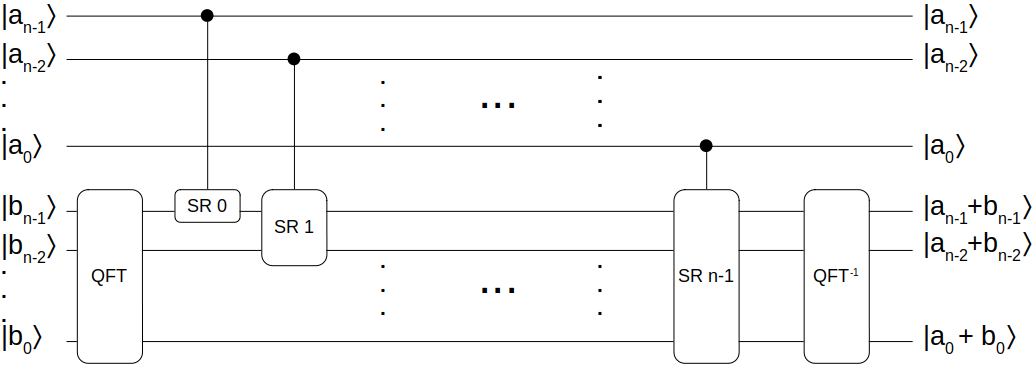
\includegraphics[width=1\textwidth]{qft-adder.png}
  \footnotesize
  \Qcircuit @C=0.35em @R=0.55em {
     & \qw & \gate{\texttt{SR}\;0} & \multigate{3}{\texttt{SR}\;1} & \qw & \qw & \qw & \multigate{5}{\texttt{SR}\;(n-1)} & \qw  \\
      & & & & & \dots & & &  \\
      & \qw & \qw  &  \ghost{\texttt{SR}\; 1} & \qw & \qw & \qw & \ghost{\texttt{SR}\;(n-1)} & \qw \\
      & & & & & & & &  \\
     & & & & & & & &  \\
   & \qw & \qw & \qw & \qw & \qw & \qw & \ghost{\texttt{SR}\;(n-1)}  & \qw 
    }
\end{minipage}
&  
\begin{minipage}{0.25\textwidth}
  \footnotesize
  \Qcircuit @C=0.25em @R=0.35em {
    & \qw & \multigate{3}{(x-a)_n} & \qw \\
    & \vdots & & \\
    & & & \\
    & \qw & \ghost{(x+a)_n} & \qw \\
    }
  \end{minipage}
&
\begin{minipage}{.45\textwidth}
% 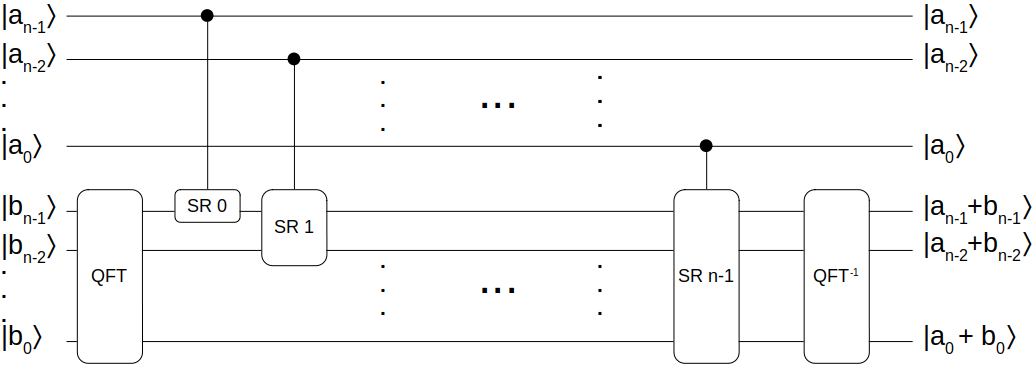
\includegraphics[width=1\textwidth]{qft-adder.png}
  \footnotesize
  \Qcircuit @C=0.35em @R=0.55em {
    & \qw & \multigate{5}{\texttt{SR}^{-1} (n-1)} & \qw & \qw & \qw & \multigate{3}{\texttt{SR}^{-1} 1} & \gate{\texttt{SR}^{-1} 0} & \qw \\
    &     &                                  &     & \dots &   &                              &                      &   \\
    & \qw & \ghost{\texttt{SR}^{-1} (n-1)}        & \qw & \qw   & \qw & \ghost{\texttt{SR}^{-1} 1} & \qw & \qw  \\
      & & & & & & & &  \\
     & & & & & & & &  \\
    & \qw & \ghost{\texttt{SR}^{-1} (n-1)} & \qw & \qw & \qw & \qw & \qw & \qw 
    }
\end{minipage}
\end{tabular}
\caption{Addition/subtraction circuits are inverses}
\label{fig:circuit-add-sub}
\end{figure}

\oqasm programs are easily invertible, as shown by the rules in \Cref{fig:exp-reversed-fun}.
This inversion operation is useful for constructing quantum oracles; for example, the core logic in the QFT-based subtraction circuit is just the inverse of the core logic in the addition circuit (\Cref{fig:exp-reversed-fun}).
This allows us to reuse the proof of addition in the proof of subtraction.
The inversion function satisfies the following properties:

 \begin{theorem}\label{thm:reversibility}\rm[Type reversibility]
    For any well-typed program $\instr$, such that $\Sigma; \Omega \vdash \instr \triangleright \Omega'$, its inverse $\instr'$, where $\instr \xrightarrow{\text{inv}} \instr'$, is also well-typed and we have $\Sigma;\Omega' \vdash \instr' \triangleright \Omega$. Moreover, $\llbracket \instr ; \instr' \rrbracket \varphi=\varphi$.
 \end{theorem}



\section{The full definitions of \qafny}
\label{sec:qafny-app}


\subsection{\qafny Session Generation}\label{sec:session-gen}

\begin{figure}[t]
{\Small
  \begin{mathpar}
    \inferrule[ ]{ }{\Omega \vdash x : \Omega(x)}



    \inferrule[ ]{\Omega(x)=(x,0,\Sigma(x)) }{\Omega \vdash x[n] : [(x,n,n+1)]}

    \inferrule[ ]{ \Omega \vdash a_1 : q_1 \\ \Omega \vdash a_2 : q_2 }{\Omega \vdash a_1 + a_2 : q_1 \sqcup q_2}   

    \inferrule[ ]{ \Omega \vdash a_1 : q_1 \\ \Omega \vdash a_2 : q_2 }{\Omega \vdash a_1 * a_2 : q_1 \sqcup q_2}   
 

    \inferrule[ ]{ \Omega \vdash a_1 : q_1 \\ \Omega \vdash a_2 : q_2 \Omega \vdash a_3 : q_3  }{\Omega \vdash (a_1 = a_2)@x[n] : q_1 \sqcup q_2\sqcup q_3}   

    \inferrule[ ]{ \Omega \vdash a_1 : q_1 \\ \Omega \vdash a_2 : q_2 \Omega \vdash a_3 : q_3  }{\Omega \vdash (a_1 < a_2)@x[n] : q_1 \sqcup q_2\sqcup q_3}

    \inferrule[ ]{ \Omega \vdash b : q}{\Omega \vdash \neg b : q}  

    \inferrule[ ]{ \Omega \vdash e : \zeta_2 \sqcup \zeta_1 }{\Omega \vdash e : \zeta_1 \sqcup \zeta_2}   

  \end{mathpar}
}
{\footnotesize
\[
\begin{array}{l}
\zeta_1 \sqcup \zeta_2 = \zeta_1 \uplus \zeta_2
\zeta \sqcup g = \zeta
\qquad 
g \sqcup \zeta = \zeta
\qquad
\cmode \sqcup \cmode = \cmode
\qquad
\qmode \sqcup \cmode = \qmode
\qquad
\cmode \sqcup \qmode = \qmode
\qquad
\cmode \le \qmode \le \zeta
\\[0.2em]
\bot \uplus l = l
\qquad 
l \uplus \bot = l

\qquad

[(x,v_1,v_2)] \uplus [(y,v_3,v_4)] = [(x,v_1,v_2), (y,v_3,v_4)]

\\

[v_2,v_2] \cap [v_3,v_4] \neq \emptyset \Rightarrow [(x,v_1,v_2)] \uplus [(x,v_3,v_4)] = [(x,\texttt{min}(v_1,v_3),\texttt{max}(v_2,v_4))]

\end{array}
\]
}
  \caption{Arith, Bool, Gate Mode Checking}
  \label{fig:exp-well-typed}
\end{figure}


A type is written as $\ttype{n}{t}$, where $n$ refers to the total number of qubits in a session,
and $t$ describes the qubit state form. 
A session being type $\ttype{n}{\tnor{\overline{d}}}$
means that every qubit is in normal basis (either $\ket{0}$ or $\ket{1}$),
and $\overline{d}$ describes basis states for the qubits.
The type corresponds to a single qubit basis state $\alpha(n)\ket{\overline{d}}$,
where the global phase $\alpha(n)$ has the form $e^{2 \pi i \frac{1}{n}}$ and $\overline{d}$ is a list of bit values.
Global phases for \texttt{Nor} type are usually ignored in many semantic definitions.
In QWhile, we record it because in quantum conditionals, such global phases might be turned to local phases.

$\ttype{n}{\thad{w}}$ means that every qubit in the session has the state: $(\alpha_1\ket{0} + \alpha_2\ket{1})$;
the qubits are in superposition but they are not entangled.
$\bigcirc$ represents the state is a uniform superposition,
while $\infty$ means the phase amplitude for each qubit is unknown.
If a session has such type, it then has the value form $\Motimes_{k=0}^{m}\ket{\Phi(n_k)}$,
where $\ket{\Phi(n_k)}=\frac{1}{\sqrt{2}}(\ket{0}+\alpha(n_k)\ket{1})$.

All qubits in a session that has type $\ttype{n}{\tch{m}{\beta}}$ are supposedly entangled (eventual entanglement below).
$m$ refers to the number of possible different entangled states in the session,
and the bitstring indexed set $\beta$ describes each of these states, while every element in $\beta$ is indexed by $i\in [0,m)$.
$\beta$ can also be $\infty$ meaning that the entanglement structure is unknown.
For example, in quantum phase estimation, after applying the $\texttt{QFT}^{-1}$ operation, the state has type $\ttype{n}{\tch{m}{\infty}}$. In such case, the only quantum operation to apply is a measurement.
If a session has type $\ttype{n}{\tch{m}{\beta}}$ and the entanglement is a uniform superposition,
we can describe its state as $\sum_{i=0}^{m}{\frac{1}{\sqrt{m}}\beta(i)}$, and the length of bitstring $\beta(i)$ is $n$.
For example, in a $n$-length GHZ application, the final state is: $\ket{0}^{\otimes n}+\ket{1}^{\otimes n}$. 
Thus, its type is $\ttype{n}{\tch{2}{\{\overline{0}^n,\overline{1}^n\}}}$, where $\overline{d}^n$ is a $n$-bit string having bit $d$.

The type $\ttype{n}{\tch{m}{\beta}}$ corresponds to the value form $\sum_{k=0}^{m}\theta_k\ket{\overline{d_k}}$.
$\theta_k$ is an amplitude real number, and $\overline{d_k}$ is the basis.
Basically, $\sum_{k=0}^{m}\theta_k\ket{\overline{d_k}}$ represents a size $m$ array of basis states
that are pairs of $\theta_k$ and $\overline{d_k}$. For a session $\zeta$ of type $\texttt{CH}$,
one can use $\zeta[i]$ to access the $i$-th basis state in the above summation, and the length is $m$.
In the Q-Dafny implementation section, we show how we can represent $\theta_k$ for effective automatic theorem proving.

The QWhile type system has the type judgment: $\Omega,\itau\vdash_g s : \zeta\triangleright \tau$, where $g$ is the context mode, mode environment $\Omega$ maps variables to modes or sessions ($q$ in \Cref{fig:vqimp}), type environment $\itau$ maps a session to its type, $s$ is the statement being typed, $\zeta$ is the session of $s$, and $\tau$ is $\zeta$'s type. 
The QWhile type system in \Cref{fig:exp-sessiontype} has several tasks. First, it enforces context mode restrictions.
Context mode $g$ is either \cmode or \qmode.
$Q$ represents the current expression lives inside a quantum conditional or loop, while \cmode refers to other cases.
In a $Q$ context, one cannot perform $M$-mode operations, i.e., no measurement is allowed.
There are other well-formedness enforcement. For example,
the session of the Boolean guard $b$ in a conditional/loop is disjoint with the session in the conditional/loop body,
i.e., qubits used in a Boolean guard cannot appear in its conditional/loop body.

Second, the type system enforces mode checking for variables and expressions in \Cref{fig:exp-well-typed}.
In QWhile, \cmode-mode variables are evaluated to values during type checking.
In a \texttt{let} statement (\Cref{fig:exp-sessiontype}),
\cmode-mode expression is evaluated to a value $n$, and the variable $x$ is replaced by $n$ in $s$.
The expression mode checking (\Cref{fig:exp-well-typed}) has the judgment: $\Omega \vdash (a\mid b) : q$. It takes a mode environment $\Omega$, and an expression ($a$, $b$), and judges if the expression has the mode $g$ if it contains only classical values, or a quantum session $\zeta$ if it contains some quantum values. 
All the supposedly \cmode-mode locations in an expression are assumed
to be evaluated to values in the type checking step,
such as the index value $x[n]$ in difference expressions in \Cref{fig:exp-well-typed}.
It is worth noting that the session computation ($\uplus$)
is also commutative as the last rule in \Cref{fig:exp-well-typed}.

Third, by generating the session of an expression, the QWhile type system assigns a type $\tau$ for the session indicating its state format, which will be discussed shortly below. Recall that a session is a list of quantum qubit fragments.
In quantum computation, qubits can entangled with each other.
We utilize type $\tau$ (\Cref{fig:vqir-state}) to state entanglement properties appearing in a group of qubits.
It is worth noting that the entanglement property refers to \textit{eventual entanglement}, .i.e. a group of qubits that are eventually entangled. Entanglement classification is tough and might not be necessary. In most near term quantum algorithms, such as Shor's algorithm \cite{shors} and Childs' Boolean equation algorithm (BEA) \cite{ChildsNAND}, programmers care about if qubits eventually become entangled during a quantum loop execution. This is why the normal basis type ($\ttype{n}{\tnor{\overline{d}}}$) can also be a subtype of a entanglement type ($\ttype{n}{\tch{1}{\{\overline{d}\}}}$) in our system (\Cref{fig:exp-subtyping}).

\myparagraph{Entanglement Types}
We first investigate the relationship between the types and entanglement states.
It is well-known that every single quantum gate application
does not create entanglement ($\texttt{X}$, $\texttt{H}$, and $\texttt{RZ}$).
It is enough to classify entanglement effects through a control gate application, i.e., 
$\sifq{x[i]}{e(y)}$, where the control node is $x[i]$ and $e$ is an operation applying on $y$.

A qubit can be described as $\alpha_1\ket{b_1}+\alpha_2\ket{b_2}$,
where $\alpha_1$/$\alpha_2$ are phase amplitudes, and $b_1$/$b_2$ are bases.
For simplicity, we assume that
when we applying a quantum operation on a qubit array $y$, we either solely change the qubit amplitudes or bases.
We identify the former one as $\mathpzc{R}$ kind, referring to its similarity of applying an \texttt{RZ} gate;
and the latter as $\mathpzc{X}$ kind, referring to its similarity of applying an \texttt{X} gate.
The entanglement situation between $x[i]$ and $y$ after applying a control statement $\sifq{x[i]}{e(y)}$ is described in \Cref{fig:control-entanglement}.

\begin{figure*}[t]
{\footnotesize
\begin{tabular}{|c|c|c|c|c|c|c|c|c|c|}
\hline                           
&  Case 1 & Case 2 & Case 3 & Case 4 & Case 5 & Case 6 & Case 7 & Case 8 & Case 9 \\
\hline
$x[i]$ & \texttt{Nor} & \texttt{Had} & \texttt{Had} & \texttt{Had} & \texttt{Had} & \texttt{Had} & \texttt{Had} & \texttt{CH} & \texttt{CH} \\
$y$  & any & \texttt{Nor} & \texttt{Nor} & \texttt{Had} & \texttt{Had} & \texttt{CH} & \texttt{CH} & \texttt{CH} & \texttt{CH}   \\\hline
$y$'s operation type  & any & $\mathpzc{X}$ & $\mathpzc{R}$ & $\mathpzc{X}$ & $\mathpzc{R}$ & $\mathpzc{X}$ & $\mathpzc{R}$ &  $\mathpzc{X}$ & $\mathpzc{R}$ \\\hline
Output Type Entangled?  & N & Y & N & N & Y & Y & Y & Y & Y  \\
\hline                           
\end{tabular}
  \caption{Control Gate Entanglement Situation}
  \label{fig:control-entanglement}
}
\end{figure*}

If $x[i]$ has input type \texttt{Nor}, the control operation acts as a classical conditional, i.e., no entanglement is possible.
In most quantum algorithms, $x[i]$ will be in superposition (type \texttt{Had}) to enable entanglement creation.
When $y$ has type $\texttt{Nor}$, if $y$'s operation is of $\mathpzc{X}$ kind, an entanglement between $x[i]$ and $y$ is created, such as the GHZ algorithm; 
if the operation is of $\mathpzc{R}$ kind, there is not entanglement after the control application, such as the Quantum Phase Estimation (QPE) algorithm.

When $x[i]$ and $y$ are both of type \texttt{Had}, if we apply an $\mathpzc{X}$ kind operation on $y$,
it does not create entanglement. An example application is the phase kickback pattern.
If we apply a $\mathpzc{R}$ operation on $y$, this does create entanglement.
This kind of operations appears in state preparations, such as preparing a register $x$ to have state $\sum_{t=0}^N i^{-t}\ket{t}$ in Childs' Boolean equation algorithm \cite{ChildsNAND}. 
The main goal for preparing such state is not to entanglement qubits, but to prepare a state with phases related to its bases.

\begin{figure}[t]
{\small
$
\begin{array}{l}
\ttype{n}{\tnor{\overline{d}}} \sqsubseteq \ttype{n}{\tch{1}{\{\overline{d}\}}}
\qquad 
\ttype{n}{\tch{2^n}{\beta}} \sqsubseteq \ttype{n}{\tch{2^n}{\infty}}
\qquad 
\ttype{n}{\thad{\bigcirc}} \sqsubseteq \ttype{n}{\tch{2^n}{\tpower{n}}}
\end{array}
$
}
  \caption{Session Type Subtyping}
  \label{fig:exp-subtyping}
\end{figure}

The case when $x[i]$ and $y$ has type \texttt{Had} and \texttt{CH}, respectively,
happens in the middle of executing a quantum loop, such as in the Shor's algorithm and BEA.
Applying both $\mathpzc{X}$ and $\mathpzc{R}$ kind operations result in entanglement.
In this narrative, algorithm designers intend to
merge an additional qubit $x[i]$ into an existing entanglement session $y$.
$x[i]$ is commonly in uniform superposition,
but there can be some additional local phases attached with some bases,
which we named this situation as saturation, i.e.,
In an entanglement session written as $\sum_{i=0}^n \ket{x_l,y,x_r}$,
for any fixing $x_l$ and $x_r$ bases, if $y$ covers all possible bases,
we then say that the part $y$ in the entanglement is in saturation.
This concept is important for generating auto-proof, which will be discussed in \Cref{sec:logical}.


When $x[i]$ and $y$ are both of type \texttt{CH}, there are two situations.
When the two parties belong to the same entanglement session,
it is possible that an $\mathpzc{X}$ or $\mathpzc{R}$ operation de-entangles the session.
Since QWhile tracks eventual entanglement.
In many cases, \texttt{HAD} type can be viewed as a kind of entanglement.
In addition, the QWhile type system make sure that most de-entanglements happen
at the end of the algorithm by turning the qubit type to $\tch{m}{\infty}$,
so that after the possible de-entanglement, the only possible application is a measurement.

If $x[i]$ and $y$ are in different entanglement sessions,
the situation is similar to when $x[i]$ having \texttt{Had} and $y$ having \texttt{CH} type.
It merges the two sessions together through the saturation $x[i]$.
For example, in BEA, The quantum Boolean guard computes the following operation $(z < i) @ x[i]$
on a \texttt{Had} type variable $z$ (state: $\sum_{k=0}^{2^n}\ket{k}$)
and a $\texttt{Nor}$ type factor $x[i]$ (state: $\ket{0}$).
The result is an entanglement $\sum_{k=0}^{2^n}\ket{k,k < i}$,
where the $x[i]$ position stores the Boolean bit result $k < i$. \footnote{When $k<i$, $x[i]=1$ while $\neg (k<i)$, $x[i]=0$.}
The algorithm further merges the $\ket{z,x[i]}$ session with a loop body entanglement session $y$. 
In this cases, both $\ket{z,x[i]}$ and $y$ are of \texttt{CH} type. 


\section{A Complicated Type System}\label{sec:newtype}

\begin{figure}
{\small
{\hspace*{-6em}
\begin{minipage}[t]{0.4\textwidth}
\begin{center}
 \[
  \begin{array}{l@{~}cl}
  \tnor{\infty} &\sqsubseteq_n& \tch{\infty}\\
  \tnor{c} &\sqsubseteq_n& \tch{\{c\}}\\
  \tch{\overline{c}(1)} &\sqsubseteq_n& \tnor{\overline{c}[0]}\\
  \thad{p} &\sqsubseteq_n& \tch{\{\tos{j}|j\in[0,2^n)\}(2^n)}\\
  \tch{\{0,1\}} &\sqsubseteq_1& \thad{\infty}\\
  \tch{p} &\sqsubseteq_n& \tch{\infty}
    \end{array}
  \]
\end{center}
\subcaption{Subtyping}
  \label{fig:qafny-subtype}
\end{minipage}
\qquad
\begin{minipage}[t]{0.45\textwidth}
\begin{center}
   \[
   \begin{array}{l@{~}cl}
  \ket{c} &\equiv_n& \sch{1}{ }{c}\\
  \sch{1}{z_j}{c_j} &\equiv_n& \ket{c_0}\\
  \shad{2^n}{n}{\alpha(r_j)} &\equiv_n& \sch{2^n}{\frac{\alpha(\sum_{k=0}^{n} r_k \cdot \tos{j}[k])}{\sqrt{2^n}}}{j}\\
  \sch{2}{z_j}{c_j} &\equiv_1& \shad{2}{1}{\frac{\sqrt{2}z_1}{z_0}}\\
   &&\qquad\texttt{when }c_0=0\;\;c_1=1
    \end{array}
 \]
\end{center}
\subcaption{State Equivalence}
  \label{fig:qafny-sequiv}
\end{minipage}
  \caption{\qafny type/state relations. $\overline{c}[n]$ produces the $n$-th element in set $\overline{c}$. $\{\tos{j}|j\in[0,2^n)\}(2^n)$ defines a set $\{\tos{j}|j\in[0,2^n)\}$ with the emphasis that it has $2^n$ elements. $\{0,1\}$ is a set of two single element bitstrings $0$ and $1$. $\cdot$ is the multiplication operation, $\tos{j}$ turns a number $j$ to a bitstring, $\tos{j}[k]$ takes the $k$-th element in the bitstring $\tos{j}$, and $\ket{j}$ is an abbreviation of $\ket{\tos{j}}$.}
  \label{fig:qafny-eq}
}
}
\end{figure}

The \qafny element component syntax is represented according to the grammar in \Cref{fig:qafny-state}. 
In \qafny, there are three kinds of values, two of which are classical ones represented by the two modes: $\cmode$ and $\mmode$.
The former represents classical values, represented as a natural number $n$, that do not intervene with quantum measurements and are evaluated in the compilation time, the latter represents values, represented as a pair $(r,n)$, produced from a quantum measurement. The real number $r$ is a characteristic representing the theoretical probability of the measurement resulting in the value $n$.
Any classical arithmetic operation does not change $r$, i.e., $(r,n)+m=(r,n+m)$. 

Quantum variables are defined as kind $\qmode{n}$, where $n$ is the number of qubits in a variable representing as a qubit array. Quantum values are more often to be described as sessions ($\lambda$) that can be viewed as clusters of possibly entangled qubits, where the number of qubits is exactly the session length, i.e., $\slen{\overline{x[n..m]}}$.
Each session consists of different disjoint ranges, connected by the $\uplus$ operation (meaning that different ranges are disjoint), represented as $x[n..m]$ that refers the number range $[n,m)$ in a quantum array named $x$. For simplicity, we assume that different variable names referring to different quantum arrays without aliasing. Sessions have associated equational properties. They are associative and identitive with the identity operation as $\bot$. There are another two equational properties for sessions below:

{\small
\[n \le j < m \Rightarrow x[n,m]\uplus\lambda \equiv_{\lambda} x[n,j]\uplus x[j,m] \uplus\lambda
\qquad 
x[n,n] \equiv_{\lambda} \bot
\]
}

Each length-$n$ session is associated to a quantum state that can be one of the three forms ($q$ in \Cref{fig:qafny-state}) that are corresponding to three different types ($\tau$ in \Cref{fig:qafny-state}). The first kind of state is of \texttt{Nor} type ($\tnor{(\topt{c})}$), having the state form $\ket{c}$, which is a computational basis value. $c$ is of length $n$ and represents a tensor product of qubits, all being $0$ or $1$. The second kind of state is of \texttt{Had} type ($\thad{(\topt{\bigcirc})}$),  meaning that qubits in such session are in superposition but not entangled.
The state form is $\shad{2^n}{n}{\alpha(r_j)}$, where $\alpha(r_j)$ is a local phase for the $j$-th qubit in the session. If $r_j=0$ for all $j$, the state can be represented by  type $\thad{\bigcirc}$ representing a uniformly distributed superposition; otherwise, we represent the type as $\thad{\infty}$. The third kind of state is of $\texttt{CH}$ type ($\tch{(\topt{\overline{c}(m)})}$), having the state form $\sch{m}{z_j}{c_j}$, referring to that qubits in such session are possibly entangled. The state $\sch{m}{z_j}{c_j}$ can be viewed as an $m$ element set of pairs $z_j\ket{c_j}$, where $z_j$ and $c_j$ are the $j$-th amplitude and basis.
The well-formed restrictions for the state are three: 1) $\sum_{j=0}^{m}|z_j|^2=1$ ($z_j$ is a complex number); 2) length of $c_j$ is $n$ for all $j$ and $m \le 2^n$; 3) any two bases $c_j$ and $c_k$ are distinct if $j \neq k$.

In \qafny, the quantum types and states are associated through bases and equational properties.
For each quantum state $q$, especially for \texttt{Nor} type state $\ket{c}$ and \texttt{CH} type state $\sch{m}{z_j}{c_j}$, the type factors are either $\infty$ meaning no bases can be tracked, or having the form $c$ and $\overline{c}(m)$ that track the bases of the state $\ket{c}$ and $\sch{m}{z_j}{c_j}$, respectively. For \texttt{Nor} type, this means that the type factor $c$ (in $\tnor{c}$) and the state qubit format $\ket{c}$ must be equal; for \texttt{CH} type ($\tch{\overline{c}(m)}$), if the state is $\sch{m}{z_j}{c_j}$, the $j$-th element $\overline{c}[j]$ is equal to $c_j$.
Additionally, \qafny types permit subtyping relations that correspond to state equivalent relations in \Cref{fig:qafny-eq}. 
Both subtype relation $\sqsubseteq_n$ and state equivalence relation $\equiv_n$ are parameterized by a session length number $n$, such that they establish relations between two quantum states describing a session of length $n$.
$\sqsubseteq_n$ in \Cref{fig:qafny-subtype} describes a type term on the left can be used as a type on the right. For example, a \texttt{Nor} type qubit array $\tnor{c}$ can be used as a single element entanglement type term $\tch{\{c\}}$ \footnote{If a qubit array only consists of $0$ and $1$, it can be viewed as an entanglement of unique possibility. }. 
Correspondingly, state equivalence relation $\equiv_n$ describes the two state forms to be equivalent; specifically, the left state term can be used as the right one, e.g., a single element entanglement state $\sch{1}{z_j}{c_j}$ can be used as a \texttt{Nor} type state $\ket{c_0}$ with the fact that $z_0$ is now a global phase that can be neglected.


\subsection{Type Checking: A Quantum Session Type System}\label{sec:typesystemappx}

\begin{figure}[t]
{
  \small
  \[\begin{array}{llcl} 
      \text{\oqasm Expr} & \mu\\
      \text{Parameter} & l & ::= & x \mid x[a] \\
      \text{Arith Expr} & a & ::= & x \mid v \mid a + a \mid a * a \mid ... \\
      \text{Bool Expr} & b & ::= & x[a] \mid (a = a) @ x[a] \mid (a < a) @ x[a] \mid ... \\
      \text{Predicate} & P & ::= & a = a \mid a < a \mid \lambda \mapsto q \mid P \wedge P \mid P * P \mid ... \\
      \text{Gate Expr} & op & ::= & \texttt{H} \mid \iqft[\lbrack -1 \rbrack]{}{} \\
      \text{C/M Moded Expr}& e & ::= & a \mid \sinit{a} \mid \smea{y} \mid \textcolor{red}{\sret{y,(r,n)}} \\
      \text{Statement} & s & ::= & \sskip \mid \sexp{x}{e}{s} \mid  \ssassign{l}{}{op} \mid \ssassign{\lambda}{}{\mu} 
                                 \mid \ssassign{l}{}{\sdis}
                                 \\ & & \mid & \sseq{s}{s} \mid \sifq{b}{s} \mid
                                     \sqwhile{j}{a_1}{a_2}{b}{s}
    \end{array}
  \]
}
  \caption{Core \qafny syntax. \oqasm is in \Cref{sec:qafny}. For an operator \texttt{OP}, $\texttt{OP}^{\lbrack -1 \rbrack}$ indicates that the operator has a built-in inverse available. Arithmetic expressions in $e$ are only used for classical operations, while Boolean expressions are used for both classical and quantum operations. $x[a]$ represents the $a$-th element in the qubit array $x$, while a quantum variable $x$ represents the qubit group $x[0..n]$ and $n$ is the length of $x$. }
  \label{fig:vqimpappx}
\end{figure}


\begin{figure}
{\small
\begin{center}
 \[
  \begin{array}{r@{~}c@{~}l@{~}cl}
  &&\{\bot:\tau\} \cup \sigma &\preceq& \sigma\\
  \tau\sqsubseteq_{\slen{\lambda}}\tau' &\Rightarrow& \{\lambda:\tau\} \cup \sigma &\preceq& \{\lambda:\tau'\} \cup \sigma\\
  &&\{\lambda_1\uplus l_1 \uplus l_2 \uplus \lambda_2 :\tau\} \cup \sigma &\preceq& \{\lambda_1\uplus l_2 \uplus l_1 \uplus \lambda_2 : \texttt{mut}(\tau,\slen{\lambda_1})\} \cup \sigma\\
  &&\{\lambda_1 :\tau_1\} \cup \{\lambda_2 :\tau_2\} \cup \sigma &\preceq& \{\lambda_1 \uplus \lambda_2 :\texttt{mer}(\tau_1,\tau_2)\} \cup \sigma \\
  \texttt{spt}(\tau,\slen{\lambda_1})=(\tau_1,\tau_2)&\Rightarrow&\{\lambda_1 \uplus \lambda_2 :\tau\} \cup \sigma &\preceq& \{\lambda_1 :\tau_1\} \cup \{\lambda_2 :\tau_2\} \cup \sigma
    \end{array}
  \]
\end{center}
{\footnotesize
\[
\begin{array}{l}
\texttt{pmut}((c_1.i_1.i_2.c_2),n)=(c_1.i_2.i_1.c_2) \;\;\texttt{when}\;\slen{c_1}=n
\\
\texttt{mut}(\tnor{c},n)=\tnor{\texttt{pmut}(c,n)}
\qquad
\texttt{mut}(\tch{\overline{c}(m)},n)=\tch{\{\texttt{pmut}(c,n)|c\in\overline{c}(m)\}(m)}
\qquad
\texttt{mut}(\tau,n)=\tau\;\;[\texttt{owise}]
\\
\texttt{mer}(\tnor{c_1},\tnor{c_2})=\tnor{(c_1.c_2)}
\qquad
\texttt{mer}(\thad{\bigcirc},\thad{\bigcirc})=\thad{\bigcirc}
\qquad
\texttt{mer}(T\;\infty,T\;t)=T\;\infty
\\
\texttt{mer}(\tch{\overline{c_1}(m_1)},\tch{\overline{c_2}(m_2)})=\tch{(\overline{c_1}\times \overline{c_2})(m_1*m_2)}
\\
\texttt{spt}(\tnor{c_1.c_2},n)=(\tnor{c_1},\tnor{c_2}) \;\;\texttt{when}\;\slen{c_1}=n
\qquad
\texttt{spt}(\thad{t},n)=(\thad{t},\thad{t})
\\
\texttt{spt}(\tch{\{c_j.c|j\in [0,m)\wedge |c_j|=n\}(m)},n)=(\tch{\{c_j|j\in [0,m)\wedge |c_j|=n\}(m)},\tnor{c})
\end{array}
\]
}
\caption{Type environment partial order. We use set union ($\cup$) to describe the type environment concatenation with the empty set operation $\emptyset$. $i$ is a single bit either $0$ or $1$. The $.$ operation is bitstring concatenation. $\times$ is the Cartesian product of two sets.
$T$ is either $\texttt{Nor}$, $\texttt{Had}$ or $\texttt{CH}$. }
  \label{fig:env-equiv}
}
\end{figure}

\begin{figure}[t]
{
{\Small
  \begin{mathpar}
    \inferrule[TPar]{\sigma \preceq \sigma' \\ \Omega,\sigma' \vdash_g s \triangleright \sigma''}{\Omega,\sigma \vdash_g s \triangleright \sigma'' }

    \inferrule[TEXP]{\Omega[x\mapsto \cmode],\sigma\vdash_g s[n/x] \triangleright \sigma'}{\Omega,\sigma \vdash_g \sexp{x}{n}{s} \triangleright \sigma' }

    \inferrule[TMEA]{ \Omega(y)=\qmode{j} \\ \sigma(y) = \{y[0..j]\uplus\lambda\mapsto \tau \}
     \\\\ \Omega[x\mapsto \mmode],\sigma[\lambda \mapsto \tch{\infty}]\vdash_{\cmode} s \triangleright  \sigma'}{\Omega,\sigma \vdash_{\cmode} \sexp{x}{\smea{y}}{s} \triangleright \sigma' }

    \inferrule[TA-CH]{ FV(\mu)=\lambda\\ \sigma(\lambda\uplus\lambda') = \tch{\overline{c}(m)}\\\\
  \overline{c'}=\{(\llbracket \mu \rrbracket c_1).c_2\;\bm{|}\;c_1.c_2\in\overline{c}\wedge\slen{c_1}=\slen{\lambda}\}}{\Omega,\sigma \vdash_g \ssassign{\lambda}{}{\mu} \triangleright \{\lambda\uplus\lambda':\tch{\overline{c'}(m)}\} }

    \inferrule[TMEA-N]{ \Omega(y)=\qmode{j} \\ \overline{c'}=\{c_2\;\bm{|}\;\tos{n}.c_2\in\overline{c}\wedge\slen{\tos{n}}=j\}
     \\\\ \Omega[x\mapsto \mmode],\sigma[\lambda \mapsto \tch{\overline{c'}(\slen{\overline{c'}})}]\vdash_{\cmode} s \triangleright  \sigma'}{\Omega,\sigma[y[0..j]\uplus\lambda\mapsto \tch{\overline{c}(m)}] \vdash_{\cmode} \sexp{x}{\sret{y,(r,n)}}{s} \triangleright \sigma' }

    \inferrule[TSEQ]{\Omega,\sigma\vdash_g s_1 \triangleright\sigma_1
 \\\\\Omega,\sigma[\uparrow \sigma_1]\vdash_g s_2 \triangleright\sigma_2}{\Omega,\sigma \vdash_g \sseq{s_1}{s_2}\triangleright \;\sigma_2\cup\sigma_1|_{\not\in\dom{\sigma_2}} }

    \inferrule[TLOOP]{ \forall j\in[n_1,n_2)\;.\;\Omega,\sigma[\uparrow \sigma'[j/x]]\vdash_g \sifq{b}{s} \triangleright \sigma'[\texttt{S}\;j/x] }
                  {\Omega,\sigma \vdash_g \sqwhile{\sint{x}{n_1}}{x<n_2}{b}{\dplus{x}}{s} \triangleright \sigma'[n_2/x]}


\inferrule[TIF]{ 
FV(b@x[j])=\lambda\uplus x[j,\texttt{S}\;j]\\
FV(b@x[j])\cap FV(s) =\emptyset \\\\
\sigma(\lambda\uplus x[j,\texttt{S}\;j]\uplus \lambda_1)=\tch{\overline{c}(m)}
\\
     \Omega,\sigma \vdash_{\mmode} s \triangleright \{\lambda\uplus x[j,\texttt{S}\;j]\uplus \lambda_1:\tch{\overline{c'}(m)}\}} 
{\Omega,\sigma \vdash_g \sifq{b@x[j]}{s} \triangleright \{\lambda\uplus x[j,\texttt{S}\;j]\uplus \lambda_1:\tch{\overline{c''}(m)}\} }

\inferrule[SLOOP-N]{}{(\varphi,\sqwhile{j}{n_1}{n_2}{b}{s})\longrightarrow (\varphi,\{\})}

  \end{mathpar}
}
{\footnotesize
\[
\begin{array}{l}
\overline{c''}=\{\tos{n}.1.c_2\;\bm{|}\;\tos{n}.d.c_1 \in \overline{c} \wedge \tos{n}.d.c_2 \in \overline{c'} \wedge b[\tos{n}/\lambda] \oplus d \wedge \slen{\tos{n}}=\slen{\lambda} \}
\\ \qquad\quad \cup \{\tos{n}.0.c_1\;\bm{|}\; \tos{n}.d.c_1 \in \overline{c} \wedge \neg (b[\tos{n}/\lambda] \oplus d) \wedge \slen{\tos{n}}=\slen{\lambda} \}
\\
\sigma[\uparrow \sigma'] = \sigma[\forall \lambda:\tau \in \sigma'\;.\;\tau/\lambda]
\\
\sigma|_{\not\in\dom{\sigma'}}=\{\lambda:\tau|\lambda \not\in \dom{\sigma'}\}

\end{array}
\]
}
}
  \caption{\qafny type system. $\llbracket \mu \rrbracket c$ is the \oqasm semantics of interpreting reversible expression $\mu$ in \Cref{fig:deno-sem}. Boolean expression $b$ can be $a_1=a_2$, $a_1 < a_2$ or \texttt{true}. $b[\tos{n}/\lambda]$ means that we treat $b$ as a \oqasm $\mu$ expression, replace qubits in array $\lambda$ with bits in bitstring $\tos{n}$, and evaluate it to a Boolean value.
$\sigma(y)=\{\lambda\mapsto \tau\}$ produces the map entry $\lambda\mapsto \tau$ and the range $y[0..\slen{y}]$ is in $\lambda$.
$\sigma(\lambda)=\tau$ is an abbreviation of $\sigma(\lambda)=\{\lambda\mapsto \tau\}$. $FV(-)$ produces a session by union all qubits appearing in $-$.}
  \label{fig:exp-sessiontype}
\end{figure}

In \qafny, typing is with respect to a \emph{kind environment} $\Omega$ and a \emph{finite type environment} $\sigma$,
which map \qafny variables to kinds and map sessions to types, respectively.
The typing judgment is written as $\Omega; \sigma\vdash_{g} s \triangleright \sigma'$,
which states that statements $s$ is well-typed under the context mode $g$ and environments $\Omega$ and $\sigma$,
the sessions representing $s$ is exactly the domain of $\sigma'$ as $\dom{\sigma'}$,
and $s$ transforms types for the sessions in $\sigma$ to types in $\sigma'$.
$\Omega$ describes the kinds for all program variables.
$\Omega$ is populated through \texttt{let} expressions that introduce variables,
and the \qafny type system enforces variable scope; such enforcement is neglected in \Cref{fig:exp-sessiontype} for simplicity.
We also assume that variables introduced in \texttt{let} expressions are all distinct through proper alpha conversions.
$\sigma$ and $\sigma'$ describe types for sessions referring to possibly entangled quantum clusters pointed to by quantum variables in $s$. 
$\sigma$ and $\sigma'$ are both finite and the domain of them contain sessions that do not overlap with each other; $\dom{\sigma}$ is large enough to describe all sessions pointed to by quantum variables in $s$,
while $\dom{\sigma'}$ should be the exact sessions containing quantum variables in $s$.
We have partial order relations defined for type environments in \Cref{fig:env-equiv}, which will be explained shortly.
Selected type rules are given in \Cref{fig:exp-sessiontype}; 
the rules not mentioned are similar and listed in \Cref{sec:qafny-app}.

The type system enforces five invariants.  First, well-formed and context restrictions for quantum programs.
Well-formedness means that qubits mentioned in the Boolean guard of a quantum conditional cannot be accessed in the conditional body,
while context restriction refers to the fact that the quantum conditional body cannot create (\texttt{init}) and measure (\texttt{measure}) qubits. 
For example the $FV$ checks in rule \textsc{TIF} enforces that the session for the Boolean and the conditional body does not overlap.
Coincidentally, we utilize the modes ($g$, either $\cmode$ or $\mmode$) as context modes for the type system. 
Context mode $\cmode$ permits most \qafny operations. Once a type rule turns a mode to $\mmode$, such as in the conditional body in rule \textsc{TIF}, we disallow \texttt{init} and \texttt{measure} operations. For example, rules \textsc{TMEA} and \textsc{TMEA-N} are valid only if the input context mode is $\cmode$.

Second, the type system tracks the basis state of every qubit in sessions. In rule \textsc{TA-CH}, we find that the oracle $\mu$ is applied on $\lambda$ belonging to a session $\lambda \uplus \lambda'$. Correspondingly, the session's type is $\tch{\overline{c}(m)}$, for each bitstring $c_1.c_2\in \overline{c}$, with $\slen{c_1}=\slen{\lambda}$, we apply $\mu$ on the $c_1$ and leave $c_2$ unchanged.
Here, we utilize the \oqasm semantics that describes transitions from a $\texttt{Nor}$ state to another $\texttt{Nor}$ one, and we generalize it to apply the semantic function on every element in the \texttt{CH} type.
During the transition, the number of elements $m$ does not change.
Similarly, applying a partial measurement on range $y[0..j]$ of the session $y[0..j]\uplus\lambda$ in rule \textsc{TMEA-N}
can be viewed as a array filter, i.e., for an element $c_1.c_2$ in set $\overline{c}$ of the type $\tch{\overline{c}(m)}$, with $\slen{c_1}=j$, we keep only the ones with $c_1=\tos{n}$ ($n$ is the measurement result) in the new set $\overline{c'}$ and recompute $\slen{\overline{c'}}$. In \qafny, the tracking procedure is to generate symbolic predicates that permit the production of the set $\overline{c'}(\slen{c'})$, not to actually produce such set. If the predicates are not not effectively trackable, we can always use $\infty$ to represent the set.


\liyi{may be we can add a rule about turning NOR to HAD so that we can say that the subtyping casting is also useful. }
Third, the type system enforces equational properties of 
quantum qubit sessions through a partial order relation over type environments, including subtyping, qubit position mutation, merge and split quantum sessions.
Essentially, we can view two qubit arrays be equivalent if there is a bijective permutation on the qubit positions of the two.
To analyze a quantum application on a qubit array, if the array is arranged in a certain way, the semantic definition will be a lot more trivial than other arrangements. For example, in applying a quantum oracle to a session (rule \textsc{TMEA}), we fix the qubits that permits the $\mu$ operation to always live in the front part ($\lambda$ in $\lambda\uplus\lambda'$).
This is achieved by a consecutive application of the mutation rule ($\texttt{mut}$) in the partial order ($\preceq$) in \Cref{fig:env-equiv}, which casts the left type environment to the format on the right through rule \textsc{TPar}.
Similarly, split ($\texttt{spt}$) and combination ($\texttt{mer}$) of sessions in \Cref{fig:env-equiv} are useful to describe some quantum operation behaviors. the split of a quantum session into two represents the process of disentanglement of quantum qubits.
For example, $\ket{00}+\ket{10}$ can be disentangled as $(\ket{0}+\ket{1})\otimes \ket{0}$.
The \texttt{spt} function is a partial one since disentanglement is considered to be a hard problem and it is usually done through case analyses as the ones in \Cref{fig:env-equiv}.
Merging two sessions is valuable for analyzing the behavior of quantum conditionals.
In rule \textsc{TIF}, the session ($\lambda_1\uplus x[j,\texttt{S}\;j]$) for the Boolean guard ($b@x[j]$)
 and the session for ($\lambda_2$) the body can be two separative sessions. 
Here, we first merge the two session through the $\texttt{mer}$ rule in \Cref{fig:env-equiv} by computing the Cartesian product of the two type bases, such that if the two sessions are both \texttt{CH} types $\lambda_1\uplus x[j,\texttt{S}\;j]\mapsto\tch{\overline{c_1}(m_1)}$ and $\lambda_2\mapsto\tch{\overline{c_2}(m_2)}$, the result is of type $\tch{(\overline{c_1}\times \overline{c_2})(m_1*m_2)}$. 
After that, the quantum conditional behavior can be understood as applying a partial map function on the size $m_1*m_2$ array of bitstrings, and we only apply the conditional body's effect on the second part (the $\overline{c_2}$ part) of some bitstrings whose first part is checked to be true by applying the Boolean guard $b$. 
\liyi{see how to merge the following to above}
Based on the new \texttt{CH} type with the set $\overline{c_1}\times \overline{c_2}$,
the quantum conditional creates a new set based on $\overline{c_1}\times \overline{c_2}$, i.e., for each element $\tos{n}.d.c$ in the set, with $\slen{\tos{n}}=\slen{\lambda_1}$, we compute Boolean guard $b$ value by substituting qubit variables in $b$ with the bitstring $\tos{n}$, and the result $b[\tos{n} / \lambda_1] \oplus d$ is true or not ($d$ represents the bit value for the qubit at $x[j,\texttt{S}\;j]$); if it is true, we replace the $c$ bitstring by applying the conditional body on it; otherwise, we keep $c$ to be the same.
In short, the quantum conditional behavior can be understood as applying a partial map function on an $m$ array of bitstrings, and we only apply the conditional body's effect on the second part of some bitstrings whose first part is checked to be true by applying the Boolean guard $b$.

Fourth, the type system enforces that the $\cmode$ classical variables can be evaluated to values in the compilation time. \footnote{We consider all computation that only needs classical computer is done in the compilation time.}, while tracks $\mmode$ variables which represent the measurement results of quantum sessions. Rule \textsc{TEXP} enforces that a classical variable $x$ is replaced with its assignment value $n$ in $s$. The substitution statement $s[n/x]$ also evaluates classical expressions in $s$, which is described in \Cref{sec:qafny-app}.
In measurement rules (\textsc{TMEA} and \textsc{TMEA-N}), we apply some gradual typing techniques.
There is an ghost expression $\texttt{ret}$ generated from one step evaluation of the measurement.
Before the step evaluation, rule \textsc{TMEA} types the partial measurement results as a classical $\mmode$ mode variable $x$ and a possible quantum leftover $\lambda$ as $\tch{\infty}$.
After the step is transitioned, we know the exact value for $x$ as $(r,n)$, so that we carry the result to type $\lambda$ as $\tch{\overline{c'}(\slen{\overline{c'}})}$. This does not violate type preservation because we have the subtyping relation $\tch{\overline{c'}(\slen{\overline{c'}})} \sqsubseteq_{\slen{\lambda}} \tch{\infty}$.

Finally, the type system extracts the result type environment of a for-loop as $\sigma'[n_2/x]$ based on the extraction of a type environment invariant on the $i$-th loop step of executing a conditional $\sifq{b}{s}$ in rule \textsc{TLOOP}, regardless if the conditional is classical or quantum. 



\subsection{\qafny Semantics and Type Soundness}\label{sec:semantics}

\begin{figure}[t]
{
{\Small
  \begin{mathpar}
    \inferrule[SPar]{\varphi \equiv \varphi' }{(\varphi,s) \longrightarrow (\varphi',s) }

    \inferrule[SMEA]{\sigma(y) = y[0..k]\uplus\lambda\mapsto \sch{m}{z_j}{c_j} \\ r = \forall j\in[0,m).\;c_j=\tos{n}.c\Rightarrow \sum{\slen{z_j}^2}}{(\varphi,\sexp{x}{\smea{y}}{s} \longrightarrow (\varphi,\sexp{x}{\sret{(y,(r,n))}}{s}) }


    \inferrule[SSEQ-1]{(\varphi,s_1) \longrightarrow (\varphi',s'_1)}{(\varphi,\sseq{s_1}{s_2})\longrightarrow (\varphi',\sseq{s'_1}{s_2}) }

    \inferrule[SMEA-N]{ \varphi(y) = \{y[0..k]\uplus \lambda : \sch{m}{z_j}{c_{j1}.c_{j2}}\} \\\overline{c}=\{c_{j2}|c_{j1}=\tos{n}\}\\c_j\in \overline{c}}{(\varphi,\sexp{x}{\sret{(y,(r,n))}}{s} \longrightarrow (\varphi[x\mapsto (r,n),\lambda \mapsto \sch{\slen{\overline{c}}}{\frac{1}{\sqrt{r}}z_j}{c_j}],s)}

    \inferrule[SSEQ-2]{}{(\varphi,\sseq{\{\}}{s_2})\longrightarrow (\varphi,s_2) }

    \inferrule[SA-CH]{ \varphi(\lambda)=\{\lambda\uplus\lambda'\mapsto \sch{m}{z_j}{c_{j1}.c_{j2}}\} \\\\ \slen{c_{j1}}=\slen{\lambda}
    \\\llbracket \mu \rrbracket c_{j1} = z'_j\ket{c'_{j1}} }{ (\varphi,\ssassign{\lambda}{}{\mu}) \longrightarrow (\varphi[\lambda\uplus\lambda'\mapsto \sch{m}{z'_j\cdot z_j}{c'_{j1}.c_{j2}}],\{\}) }

    \inferrule[SEXP]{ }{(\varphi,\sexp{x}{n}{s}) \longrightarrow (\varphi,s[n/x]) }


\inferrule[SIF]{ \lambda=\lambda_1\uplus x[j,\texttt{S}\;j]\uplus \lambda_2 \\ FV(b@x[j]) = \lambda\uplus x[j,\texttt{S}\;j] \\ 
  \varphi(\lambda)=\sch{m}{z_j}{c_{j1}.c_{j2}}]
\\
(\varphi,s) \longrightarrow^* (\varphi[\lambda\mapsto \sch{m}{z'_j}{c_{j1}.c'_{j2}}],\{\}) \\ \slen{c_{j1}}=\slen{\lambda} } 
{(\varphi,\sifq{b@x[j]}{s}) \longrightarrow (\varphi[\lambda\mapsto \texttt{pmap}(m,z_j,z'_j,c_{j1},c'_{j1},c_{j2})],\{\}) }

  \end{mathpar}
}
}
  \caption{\qafny small step semantics. $\llbracket \mu \rrbracket c$ is the \oqasm semantics of interpreting reversible expression $\mu$ in \Cref{fig:deno-sem}. Boolean expression $b$ can be $a_1=a_2$, $a_1 < a_2$ or \texttt{true}.
$\varphi(y)=\{\lambda\mapsto q\}$ produces the map entry $\lambda\mapsto q$ and the range $y[0..\slen{y}]$ is in $\lambda$.
$\varphi(\lambda)=q$ is an abbreviation of $\varphi(\lambda)=\{\lambda\mapsto q\}$.}
  \label{fig:exp-semantics}
\end{figure}

We define the semantics of an \oqasm program as a partial function
$\llbracket\rrbracket$ from
an instruction $\instr$ and input state $\varphi$ to an output state
$\varphi'$, written 
$\llbracket \instr \rrbracket\varphi=\varphi'$, shown in \Cref{fig:deno-sem}.
% The definition for $\llbracket\rrbracket$ is syntax-driven, meaning that it is defined in terms of the state syntax presented in \Cref{fig:vqir-state}.

% defines the denotational semantics of \oqasm, which maps a \oqasm instruction $\instr \in \{\instr\}$ to its unitary operator on $\varphi \in \hsp{S}^d$.

% The key takeaway of the \oqasm denotational semantics is that given an input $\varphi \in \hsp{S}^d$, a well typed instruction affects only one qubit (notation: $\varphi{(x,n)}$ or $q_{(x,n)}$) or qubit array (notation: $\varphi{(x)}$ or $q_x$), which means it \emph{does not create entanglement}.
% The benefit of this is that we can completely describe the state $\varphi$ using $d$ terms, instead of considering a length $2^d$ vector, as would generally be required to analyze an $d$-qubit system.

Recall that a state $\varphi$ is a tuple of $d$ qubit values,
modeling the tensor product $q_1\otimes \cdots \otimes q_d$. 
The rules implicitly map each variable $x$ to a
range of qubits in the state, e.g., 
$\varphi(x)$ corresponds to some sub-state $q_k\otimes \cdots \otimes q_{k+n-1}$
where $\Omegasz(x)=n$.
%
Many of the rules in \Cref{fig:deno-sem} update a \emph{portion} of a
state. We write $\app{q_{(x,i)}}{\varphi}{(x,i)}$ to update the $i$-th
qubit of variable $x$ to be the (single-qubit) state $q_{(x,i)}$, and
$\app{q_{x}}{\varphi}{x}$ to update variable $x$ according to
the qubit \emph{tuple} $q_x$.
$\app{\uparrow q_{(x,i)}}{\varphi}{(x,i)}$ and $\app{\uparrow q_{x}}{\varphi}{x}$ 
are similar, except that they also accumulate the previous global phase of $\varphi(x,i)$ (or $\varphi(x)$).
We use $\downarrow$ to convert a qubit $\alpha(b)\overline{q}$ to an unphased qubit $\overline{q}$.
%Thus, we have $\downarrow \alpha(b)\overline{q}=\overline{q}$ 
%and $\downarrow (q_1\otimes...\otimes q_n) = \downarrow q_1\otimes...\otimes \downarrow q_n$. 
%$\app{\uparrow q_{(x,i))}}{\varphi}{(x,i)}$ means to put back the global phase to the result qubit assigning to $(x,i)$. 
%%If $\varphi(x,i)=e^{2\pi i b}\overline{q}$ 
%and the result $q_{(x,i)}=\overline{q_{(x,i)}}$, 
%then we assign $e^{2\pi i b}\overline{q_{(x,i)}}$ to $(x,i)$;
%if the result $q_{(x,i)}=e^{2\pi i b_1}\overline{q_{(x,i)}}$, then we assign $e^{2\pi i (b+b_1)}\overline{q_{(x,i)}}$ to $(x,i)$. $\app{\uparrow q_{x}}{\varphi}{x}$ applies the above scenario to a list of qubits $q_k\otimes ... \otimes q_{k+n-1}$
%where $\Omegasz(x)=n$.

Function $\xsem$ updates the state of a single
qubit according to the rules for the standard quantum gate $X$.  
\texttt{cu} is a conditional operation
depending on the \texttt{Nor}-basis qubit $(x,i)$. 
\texttt{SR} (or
$\texttt{SR}^{-1}$) applies an $m+1$ series of \texttt{RZ} (or
$\texttt{RZ}^{-1}$) rotations where the $i$-th rotation
applies a phase of $\alpha({\frac{1}{2^{m-i+1}}})$
(or $\alpha({-\frac{1}{2^{m-i+1}}})$).
$\qsem$ applies an approximate quantum Fourier transform; $\ket{y}$ is an abbreviation of
$\ket{b_1}\otimes \cdots \otimes \ket{b_i}$ (assuming $\Omegasz(y)=i$)
and $n$ is the degree of approximation.
If $n = i$, then the operation is the standard QFT\@.
Otherwise, each qubit in the state is mapped to $\qket{\frac{y}{2^{n-k}}}$, which is equal to $\frac{1}{\sqrt{2}}(\ket{0} + \alpha(\frac{y}{2^{n-k}})\ket{1})$ when $k < n$ and $\frac{1}{\sqrt{2}}(\ket{0} + \ket{1}) = \ket{+}$ when $n \leq k$ (since $\alpha(n) = 1$ for any natural number $n$).
$\qsem^{-1}$ is the inverse function of $\qsem$. 
Note that the input state to $\qsem^{-1}$ is guaranteed to have the form $\bigotimes_{k=0}^{i-1}(\qket{\frac{y}{2^{n-k}}})$ because it has type $\tphi{n}$.
$\psem_l$, $\psem_r$, and
$\psem_a$ are the semantics for \itext{Lshift}, 
\itext{Rshift}, and \itext{Rev}, respectively.   
% Several takeaways about \oqasm denotational semantics.
% For any operation application within the space domain $\hsp{S}^d$, the semantic application $U$ only has effect on the specific qubit ($\varphi_{(x,n)}$) / qubit array ($\varphi_{x}$) that it targets at, which does not create entanglement with other subsystems.
% This clear separation only works for the domain $\hsp{S}^d$.
% When we compile these operations to \sqir and see their effects on a general Hilbert space $\hsp{H}$, they might have entanglement effects.
% \yxp{Even if we turn it into unitary over the Hilbert space, it still does not generate entanglement with other subsystems.}
% \liyi{Can you have CNOT x y when you have x is Had and y is in Nor, then you will definitely have entanglement. }
% However, the clear separation in $\hsp{S}^d$ provides us a decompositional and analytical way of verifying and validating quantum oracles; thus, each sub-oracle-component can be analyzed individually. The potential entanglements in a general Hilbert space becomes the naturally extended (additive) superposition effects.
% In addition, all semantic functions in Fig.~\ref{fig:deno-sem} are carefully engineered to only target qubits in a register $\varphi$, and does not target on invidual vectors in the vector space $\varphi$ represents.
% For example, $\xsem$ is defined for a basis phase space case $\ket{c}$, and we also define the case for superposition $\frac{1}{\sqrt{2}}(\ket{0}+(-1)^c\ket{1})$. We do not assume the the semantics of the basis phase space is automatically extended to dealing with individual elements in the superposition case.
% By using the semantics to prove quantum oracle properties, we only need to consider $O(n)$ qubits instead of the possible $2^n$ expanded vector elements.
% The semantics of a universal quantum assembly language like \sqir, by contrast, represents a quantum state as a unitary matrix whose size is \emph{exponential} in the number of vectors by expanding qubits to vectors in a register. \sqir's semantics also relies on the use of concrete qubits; using a unitary matrix and virtual positions would inject a virtual-to-physical mapping into the semantic definition, which can severely complicate proofs~\cite{PQPC}. This leads to the successful correctness proof of the QFT-adder for the first time (Sec.~\ref{sec:op-verification}).
% We only define semantic functions for qubit forms when it is possible to apply. For example, we do not define $\xsem$ for the form $\frac{1}{\sqrt{2}}(\ket{0}+e^{2\pi{i} b}\ket{1})$, because the \oqasm type system does not allow it. 

\ignore{
\begin{figure*}[t]
{\footnotesize
  \begin{mathpar}

    \inferrule[PA-NOR ]{(\itau ,\itau')\models_g (T,\ssassign{\overline{l}}{}{a},T'):\zeta\triangleright\ttype{n}{\tnor{\overline{d}}}}
                {\Omega\vdash_g\fivepule{T}{P[\llbracket a \rrbracket \zeta /\zeta] } {\ssassign{\overline{l}}{}{a}} {T'}{P}}


    \inferrule[PA-CH ]{(\itau,\itau')\models_g (T,\ssassign{\overline{l}}{}{a},T'):\zeta\uplus\zeta'\triangleright \ttype{n}{\tch{m}{\beta}}
                 \\ \itau(\overline{l})=\zeta}
       {\Omega\vdash_g\fivepule{T}{P[\forall k < m.\;\llbracket a \rrbracket(\zeta[k]) / \zeta[k]] } {\ssassign{\overline{l}}{}{a}}{T'}{P}}


    \inferrule[P-MEA ]{ (\itau[\forall \zeta'\;.\;\zeta\uplus\zeta' \mapsto \ttype{n+n'}{\tch{(m\times m')}{(\beta\cdot\beta')}}],\itau'[\forall \zeta'\;.\;\zeta' \mapsto \ttype{n'}{\tch{m'}{\beta'}}])\models_{\cmode} (T,y,T''):\zeta\triangleright \ttype{n}{\tch{m}{\beta}}
  \\ v < m \\
   \Omega[x\mapsto M,y\mapsto \bot]\vdash_{\cmode} \fivepule{T''}{P[(\iasa{2}{\zeta[v]},\ibs{\zeta[v]}) /x, \bot / \zeta] } {s} {T'}{Q} } {\Omega\vdash_{\cmode}\fivepule{T}{P}{\sexp{x}{\smea{y}}{s}}{T'}{Q}}

    \inferrule[P-IF ]{(\itau,\itau')\models_{\qmode} (T,s,T'):\zeta'\triangleright \ttype{n'}{\tch{m'}{\beta'}}
      \\\Omega\vdash b(@x[v]): \zeta\uplus[(x,v,v+1)] \\ \itau(\zeta\uplus[(x,v,v+1)])= \ttype{n}{\tch{2m}{(\beta_1\cdot 0 \cup \beta_2\cdot 1)}}
       }{\Omega\vdash_{g}\fivepule{T}{P[(\zeta\uplus 0 \uplus \zeta')\texttt{++}(\zeta\uplus 1 \uplus \llbracket s \rrbracket\zeta') /\zeta\uplus[(x,v,v+1)]\uplus\zeta'] }
      {\sifq{b(@x[v])}{s}}{T'}{P}}
    
    \inferrule[P-DIS ]{(\itau,\itau')\models_g (T,\sdistr{x},T'):\zeta\triangleright \ttype{n'}{\tch{m'}{\beta'}}
             \\ \itau(x)=\{\zeta:\ttype{n'}{\tch{m}{\beta}}\}
    \\\zeta = \zeta' \uplus (x,0,\Sigma(x))
    \\ \beta_1 \cdot \beta_2=\beta(\downarrow (x,0,\Sigma(x)))\cdot \beta(\downarrow \zeta') } 
           {\Omega\vdash_g\fivepule{T}{P[\texttt{dis}(n',\zeta,\beta,\beta_1,\beta_2) /\zeta] }
      {\sdistr{x}}{T'}{P}}


  \end{mathpar}
}
{\footnotesize
\[
\begin{array}{l}
\texttt{ln}(\zeta)\text{: length of }\zeta
\qquad
\texttt{as}(\zeta[v])\text{: the amplitude of }\zeta[v]
\qquad
\texttt{bs}(\zeta[v])\text{: the base of }\zeta[v]
\qquad
\texttt{++}\text{: array concatenation.}
\\
\texttt{dis}(n,\zeta,\beta,\beta_1,\beta_2)\equiv \{\frac{1}{2^{n-1}}(\sum_k \texttt{as}(\zeta[k])-\texttt{as}(\zeta[j]))\beta_1[j]
                           \;|\; \beta_1[j]\in \tpower{n} \}
\\
\qquad\qquad\qquad\qquad\qquad
\cup  \bigcup_{j\in \beta_2}\{\frac{1}{2^{n}}\sum_k \texttt{as}(\zeta[k])z
                           \;|\; z\in \tpower{n} \wedge (\forall k.\;z \cdot \beta_2[j] \neq \beta[k]) \}
\end{array}
\]
}
\caption{Selected Proof System Rules}
\label{fig:exp-proofsystem}
\end{figure*}
}
\subsection{Logic Proof System}\label{sec:logical}


The reason of having the session type system in \Cref{fig:exp-sessiontype}
is to enable the proof system given in \Cref{fig:exp-proofsystem}.
Every proof rule is a structure as $\Omega\vdash_g \fivepule{T}{P}{s}{T'}{Q}$,
where $g$ and $\Omega$ are the type entities mentioned in \Cref{sec:typesystem}.
$T$ and $T'$ are the pre- and post- type predicates for the statement $s$, 
meaning that there is type environments $\itau$ and $\itau'$, such that $\itau\models T$,
$\itau'\models T'$, $g,\Omega,\itau \vdash s : \zeta\triangleright \tau$, and $(\zeta\mapsto \tau) \in \itau'$.
We denote $(\itau,\itau')\models (T,s,T'):\zeta\triangleright\tau$ as the property described above.
$P$ and $Q$ are the pre- and post- Hoare conditions for statement $s$.

The proof system is an imitation of the classical Hoare Logic array theory.
We view the three different quantum state forms in \Cref{fig:vqir-state} as arrays with elements in different forms,
and use the session types to guide the occurrence of a specific form at a time.
Sessions, like the array variables in the classical Hoare Logic theory,
represent the stores of quantum states.
The state changes are implemented by the substitutions of sessions
with expressions containing operation's semantic transitions.
The substitutions can happen for a single index session element or the whole session.

Rule \text{PA-NOR} and \text{PA-CH} specify the assignment rules.
If a session $\zeta$ has type \texttt{Nor}, it is a singleton array,
so the substitution $\llbracket a \rrbracket \zeta /\zeta$ means
that we substitute the singleton array by a term with the $a$'s application.
When $\zeta$ has type \texttt{CH}, term $\zeta[k]$ refers to each basis state in the entanglement.
The assignment is an array map operation that applies $a$ to every element in the array.
For example, in \Cref{fig:shorexample} line 12,
we apply a series of \code{H} gates to array $x$.
Its post-condition is $[(x,0,n)]=\Motimes_{k=0}^{n}\ket{\Phi(0)}$,
where $[(x,0,n)]$ is the session representing register variable $x$.
Thus, replacing the session $[(x,0,n)]$ with the \code{H} application
results in a pre-condition as $\code{H}[(x,0,n)]=\Motimes_{k=0}^{n}\ket{\Phi(0)}$,
which means that $[(x,0,n)]$ has the state $\ket{0}^n$.

Rule \text{P-MEA} is the rule for partial/complete measurement.
$y$'s session is $\zeta$, but it might be a part of an entangled session $\zeta\uplus\zeta'$.
After the measurement, $M$-mode $x$ has the measurement result $(\ias{\zeta[v]}^2,\ibs{\zeta[v]})$ coming
from one possible basis state of $y$ (picking a random index $v$ in $\zeta$), 
$\ias{\zeta[v]}$ is the amplitude and $\ibs{\zeta[v]}$ is the base.
We also remove $y$ and its session $\zeta$ ($\bot/\zeta$) in the new pre-condition because it is measured away.
The removal means that the entangled session $\zeta\uplus\zeta'$ is replaced by $\zeta'$ 
with the re-computation of the amplitudes and bases for each term.

Rule \text{P-IF} deals with a quantum conditional where the Boolean guard $b(@x[v])$ is of type $\ttype{n}{\tch{2m}{(\beta_1\cdot 0 \cup \beta_2\cdot 1)}}$. The bases are split into two sets $\beta_1\cdot 0$ and $\beta_2\cdot 1$, where the last bit represents the base state for the $x[v]$ position.
In quantum computing, a conditional is more similar to an assignment, where we create a new array to substitute 
the current state represented by the session $\zeta\uplus[(x,v,v+1)]\uplus\zeta'$.
Here, the new array is given as $(\zeta\uplus 0 \uplus \zeta')\texttt{++}(\zeta\uplus 1 \uplus \llbracket s \rrbracket\zeta')$,
where we double the array: if the $x[v]$ position is $0$, we concatenate the current session $\zeta'$ for the conditional body,
if $x[v]=1$, we apply $\llbracket s \rrbracket$ on the array $\zeta'$ and concatenate it to $(\zeta\uplus 1)$.

Rule \text{P-Loop} is an initiation of the classical while rule in Hoare Logic with the loop guard possibly having quantum variables.
In QWhile, we only has \texttt{for-loop} structure and we believe it is enough to specify any current quantum algorithms.
For any $i$, if we can maintain the loop invariant $P(i)$ and $T(i)$ with the post-state $P(f(i))$ and $T(f(i))$
for a single conditional $\sifq{x[i]}{s}$, the invariant is maintained for multiple steps
for $i$ from the lower-bound $a_1$ to the upper bound $a_2$.

Rule \text{P-DIS} proves a diffusion operator $\sdistr{x}$.
The quantum semantics for $\sdistr{x}$ is $\frac{1}{2^{n}}(2\sum_{i=0}^{2^n}(\sum_{j=0}\alpha_j)\ket{i} - \sum_{j=0}\alpha_j\ket{x_j})$.
As an array operation, $\sdistr{x}$ with the session $\zeta$ is an array operation as follows:
assume that $\zeta=(x,0,\Sigma(x))\uplus\zeta_1$, for every $k$,
if $\zeta[k]$'s value is $\theta_k(\overline{d_x}\cdot \overline{d_1})$,
for any bitstring $z$ in $\tpower{\Sigma(x)}$, if $z\cdot \overline{d_1}$
is not a base for $\zeta[j]$ for any $j$, then the state is
$\frac{1}{2^{n-1}}\sum_{k=0}\theta_k(z\cdot \overline{d_1})$;
if the base of $\zeta[j]$ is $z\cdot \overline{d_1}$,
then the state for $\zeta[j]$ is $\frac{1}{2^{n-1}}(\sum_{k=0}\theta_k)-\theta_j(z\cdot \overline{d_1})$.



We evaluate \name by (1) demonstrating how it can be used for validation, both by verification and random testing, and (2) by showing that it gets good performance in terms of resource usage compared to Quipper, a state-of-the-art quantum programming framework~\cite{Green2013}.
%
This section presents the arithmetic operators we have implemented in
\oqasm, while the next section discusses the geometric operators and
expressions implemented in \vqimp. The following section presents an
end-to-end case study applying Grover's search.

\begin{figure}[t]
{\small
\[\hspace*{-1em}
\begin{array}{r l  l}
\textcolor{blue}{1}
&&
\{A(x) * A(y) \}
\quad\text{where}\;\;
A(\beta) = \beta[0..n] \mapsto \ket{\overline{0}} 
\\[0.2em]
&&
\qquad\qquad\qquad
\qquad\qquad\quad
\begin{array}{l}
B = 1 < a < N \wedge n > 0 \;\wedge
\\\qquad N < 2^n \wedge \texttt{gcd}(a,N)=1
\end{array}
\\[0.5em]
\textcolor{blue}{2}
&
&
\textcolor{teal}{
\Rightarrow
\{\dabs{\ihadh}(x[0..n]) \mapsto C * A(y) * B \}
}
\\[0.2em]
&&
\qquad\qquad\qquad
\qquad\;\;
\text{where}
\;\;
\textcolor{teal}{
C = \shad{2^n}{n}{}
}
\\[0.5em]
\textcolor{blue}{3}
& \ssassign{x}{}{\ihadh};
&
\textcolor{teal}{
\{x[0..n] \mapsto C * A(y) * B \}
}
\\[0.4em]
\textcolor{blue}{4}
&
&
\textcolor{teal}{
\Rightarrow
\{x[0..n] \mapsto C * \dabs{y\splus 1}(y[0..n]) \mapsto \ket{\overline{0}.1} * B \}
}
\\[0.4em]
\textcolor{blue}{5}
& \ssassign{y}{}{y\splus 1};
&
\textcolor{teal}{
\{x[0..n] \mapsto C * y[0..n] \mapsto \ket{\overline{0}.1} * B \}
}
\\[0.4em]
\textcolor{blue}{6}
& 
&
\textcolor{teal}{
\Rightarrow
\{ E(0) * B \}
}
\;\;
\texttt{where}\;\;
\textcolor{teal}{E(k) =}
\\[0.2em]
&&
\qquad\qquad\quad\;
\qquad
\textcolor{teal}{
\begin{array}{l}
x[0..n\,\sminus\,k] \mapsto \shad{2^{n \,\sminus\,  k}}{n \,\sminus\, k}{}\;*
\\[0.2em]
\{x[0..k],y[0..n]\} \mapsto \sch{2^k}{\frac{1}{\sqrt{2^k}}}{\tos{j}.\tos{a^{j}\;\%\;N}}
\end{array}
}
\\[0.4em]
\textcolor{blue}{7}
&\sqforh{\sint{j}{0}}{j\,\slt\, n}{x[j]}{\dplus{j}}
&
\{E(j) * B \}
\\[0.4em]
\textcolor{blue}{8}
&
\{\quad  \ssassign{y}{}{a^{2^j}y\;\%\; N}
&
\textcolor{teal}{
\{E(j\,\splus\, 1) * B \}
}
\\[0.4em]
\textcolor{blue}{9}
&
\}
&
\textcolor{teal}{
\{E(n) * B \}
}
\\[0.4em]
\textcolor{blue}{10}
&
&
\textcolor{teal}{
\Rightarrow
\{\{x[0..n],y[0..n]\} \mapsto \sch{2^{n}}{\frac{1}{\sqrt{2^{n}}}}{\tos{j}.\tos{a^{j}\;\%\;N}} * B \}
}
\\[0.4em]
\textcolor{blue}{11}
& \sexp{u}{\smea{y}}{...}
&
\textcolor{purple}{
\big{\{}
\begin{array}{l}
x[0..n] \mapsto \smch{\frac{1}{\sqrt{s}}}{s}{t\,\splus\,k p} 
\wedge
p = \texttt{ord}(a,N)
\\
\wedge\;
\texttt{nat}(u)=a^{t}\;\%\;N
\wedge
s=\texttt{rnd}(\frac{2^n}{p}) \wedge B
\end{array}
\big{\}}
}
\end{array}
\]
}
\caption{Pre-measurement quantum steps of the Shor's algorithm. Second half in \Cref{fig:shorqafny2}. $\snat{u}$ gets the integer number part of $u$ (mode $\mmode$). $\sord{a,N}$ gets the order of $a$ and $N$. $\srnd{r}$ rounds $r$ to the nearest integer. }
\label{fig:shorqafnyaa}
\end{figure}

\begin{figure}[t]
{\small
\[
\begin{array}{r l  l}
\textcolor{blue}{11}
&
\sexp{z}{\smea{y}}{}
&
\textcolor{purple}{
\big{\{}
\begin{array}{l}
x[0..n] \mapsto \smch{\frac{1}{\sqrt{s}}}{s}{t+jr} 
\wedge
\\
\texttt{nat}(z)=a^{n}\;\%\;N
\wedge
s=\texttt{rnd}(\frac{2^n}{r}) \wedge B
\end{array}
\big{\}}
}
\\[0.4em]
\textcolor{blue}{12}
&
\quad\ssassign{x}{}{\iqft[-1]{}{}}; 
&
\textcolor{teal}{
\big{\{}
x[0..n] \mapsto \smich{\frac{1}{\sqrt{s 2^n}}}{2^n}{(\omega^{tk}\Msum_{j=0}^{s}\omega^{tkj})}{k} 
\wedge
s=\texttt{rnd}(\frac{2^n}{r}) \wedge B
\big{\}}
}
\\[0.4em]
\textcolor{blue}{13}
&
\quad\sexp{u}{\smea{x}}{}
&
\textcolor{teal}{
\big{\{}
\texttt{nat}(u)=r \wedge \texttt{pos}(u)=\frac{4}{\pi ^ {2 r}}
\wedge
s=\texttt{rnd}(\frac{2^n}{r}) \wedge r = \texttt{ord}(a,N) \wedge B
\big{\}}
}
\\[0.4em]
\textcolor{blue}{14}
&
\quad\quad\texttt{post}(u)
&
\big{\{}
\texttt{nat}(\texttt{post}(u))=r \wedge r = \texttt{ord}(a,N) \wedge \texttt{pos}(u)=\frac{4e^{-2}}{\pi^2 \texttt{log}_2^4 N \wedge B}
\big{\}}
\end{array}
\]
}
{\footnotesize
\[
B=1 < a < N \wedge n > 0 \wedge N < 2^n \wedge \texttt{gcd}(a,N)=1
\qquad
\omega=e^{\frac{2\pi i}{2^n}}
\]
}
\caption{Second half of the Shor's algorithm quantum part in Qafny.}
\label{fig:shorqafny2}
\end{figure}


\subsection{Implemented Operators}

\Cref{fig:circ-evaluation} and \Cref{fig:op-table} tabulate the
arithmetic operators we have implemented in \vqir. 

The addition and modular multiplication circuits 
(parts (a) and (d) of \Cref{fig:circ-evaluation}) are components of the oracle used in Shor's factoring algorithm~\cite{shors}, which accounts for most of the algorithm's cost \cite{Gidney2021howtofactorbit}.
The oracle performs modular exponentiation on natural numbers via modular multiplication, which takes a quantum variable $x$ and two co-prime constants $M, N \in \mathbb{N}$ and produces $(x * M) \% N$. We have implemented two modular multipliers---inspired by \citet{qft-adder}
and \citet{ripple-carry-mod}---in \vqir. 
Both modular multipliers are constructed using controlled modular addition by a constant, which is implemented in terms of controlled addition and subtraction by a constant, as shown in \Cref{fig:mod-mult}.
The two implementations differ in their underlying adder and subtractor circuits: the first (QFT) uses a quantum Fourier transform-based circuit for addition and subtraction \cite{Draper2000AdditionOA}, while the second (TOFF) uses a ripple-carry adder \cite{ripple-carry-mod}, which makes use of classical controlled-controlled-not (Toffoli) gates.


\begin{figure}
{\footnotesize
{\hspace*{-6em}
\begin{minipage}[t]{0.35\textwidth}
\begin{center}
 \[
  \begin{array}{l@{~}cl}
  \tau & \sqsubseteq & \tau \\
  \tnort &\sqsubseteq& \tcht\\
  \thadt &\sqsubseteq& \tcht
    \end{array}
  \]
\end{center}
\subcaption{Subtyping}
  \label{fig:qafny-subtype}
\end{minipage}
\qquad
\begin{minipage}[t]{0.5\textwidth}
\begin{center}
   \[
   \begin{array}{l@{~}cl}
   q & \equiv_{\slen{q}} & q \\
  \ket{c} &\equiv_n& \sch{1}{ }{c}\\
  \shad{2^n}{n}{\alpha(r_j)} &\equiv_n& \sch{2^n}{\frac{\alpha(\sum_{k=0}^{n} r_k \cdot \tos{j}[k])}{\sqrt{2^n}}}{j}
    \end{array}
 \]
\end{center}
\subcaption{Quantum Value Equivalence}
  \label{fig:qafny-sequiv}
\end{minipage}
\hfill{}
\begin{minipage}[t]{0.8\textwidth}
\begin{center}
 \[
  \begin{array}{l @{~} c @{~} l l@{~}c @{~} l l @{~}c @{~} l l @ {~} c @{~} l}
\lambda &\equiv & \lambda
&
\qquad
x[n,n] & \equiv & \bot
&
\qquad
\bot \uplus \lambda & \equiv & \lambda
&
\qquad
x[n,m]\uplus\lambda & \equiv & x[n,j]\uplus x[j,m] \uplus\lambda
\\
&&&&&&&&&&&
\texttt{where}\;\;n \le j < m

    \end{array}
  \]
\end{center}
\subcaption{Session Equivalence}
  \label{fig:qafny-ses-equal}
\end{minipage}
\hfill{}
\hspace*{-5em}
\begin{minipage}[t]{0.475\textwidth}
\begin{center}
 \[
  \begin{array}{l@{~}c@{~}l}
    \sigma & \preceq & \sigma \\[0.2em]
  \{\bot:\tau\} \cup \sigma &\preceq& \sigma\\[0.2em]
   \{\lambda:\tau\} \cup \sigma &\preceq& \{\lambda:\tau'\} \cup \sigma\\
&&\texttt{where}\;\;\tau\sqsubseteq_{\slen{\lambda}}\tau' \\[0.2em]
  \{\lambda_1\uplus l_1 \uplus l_2 \uplus \lambda_2 :\tau\} \cup \sigma &\preceq& \{\lambda_1\uplus l_2 \uplus l_1 \uplus \lambda_2 : \tau\} \cup \sigma\\[0.2em]
  \{\lambda_1 :\tau\} \cup \{\lambda_2 :\tau\} \cup \sigma &\preceq& \{\lambda_1 \uplus \lambda_2 :\tau\} \cup \sigma \\[0.2em]
  \{\lambda_1 \uplus \lambda_2 :\tau\} \cup \sigma &\preceq& \{\lambda_1 :\tau\} \cup \{\lambda_2 :\tau\} \cup \sigma
\\
&&\texttt{where}\;\;\tau\neq\tcht
    \end{array}
  \]
\end{center}
\subcaption{Environment Equivalence}
  \label{fig:env-equiv}
\end{minipage}
\begin{minipage}[t]{0.475\textwidth}
\begin{center}
   \[
   \begin{array}{l@{~}c@{~}l}
    \varphi & \equiv & \varphi \\[0.2em]
  \{\bot:q\} \cup \varphi &\equiv& \varphi\\[0.2em]
   \{\lambda:q\} \cup \varphi &\equiv& \{\lambda:q'\} \cup \varphi\\
   &&\texttt{where}\;\;q\equiv_{\slen{\lambda}}q' 
   \\[0.2em]
  \{\lambda_1\uplus l_1 \uplus l_2 \uplus \lambda_2 :q\} \cup \varphi &\equiv& \{\lambda_1\uplus l_2 \uplus l_1 \uplus \lambda_2 : \texttt{mut}(q,\slen{\lambda_1})\} \cup \varphi\\[0.2em]
  \{\lambda_1 :q_1\} \cup \{\lambda_2 :q_2\} \cup \varphi &\equiv& \{\lambda_1 \uplus \lambda_2 :\texttt{mer}(q_1,q_2)\} \cup \varphi 
   \\[0.2em]
  \{\lambda_1 \uplus \lambda_2 :\varphi\} \cup \sigma &\equiv& \{\lambda_1 :\varphi_1\} \cup \{\lambda_2 :\varphi_2\} \cup \sigma
\\
&&\texttt{where}\;\;\texttt{spt}(\tau,\slen{\lambda_1})=(\varphi_1,\varphi_2)
    \end{array}
 \]
\end{center}
\subcaption{State Equivalence}
  \label{fig:qafny-stateequiv}
\end{minipage}
{\footnotesize
\[
\begin{array}{l}
\texttt{pmut}((c_1.i_1.i_2.c_2),n)=(c_1.i_2.i_1.c_2) \;\;\texttt{when}\;\slen{c_1}=n
\\[0.2em]
\texttt{mut}(\ket{c},n)=\ket{\texttt{pmut}(c,n)}
\\[0.2em]
\texttt{mut}(\frac{1}{\sqrt{2^m}}(q_1 \bigotimes (\ket{0}+\alpha(r_n)\ket{1}) \bigotimes (\ket{0}+\alpha(r_{n+1})\ket{1}) \bigotimes q_2),n)
\\
\qquad\qquad
=\frac{1}{\sqrt{2^m}}(q_1 \bigotimes (\ket{0}+\alpha(r_{n+1})\ket{1}) \bigotimes (\ket{0}+\alpha(r_n)\ket{1}) \bigotimes q_2)
\quad\texttt{when\;}\slen{q_1}=n
\\[0.2em]
\texttt{mut}(\sch{m}{z_j}{c_j},n)=\sch{m}{z_j}{\texttt{pmut}(c_j,n)}
\\[0.2em]
\texttt{mer}(\ket{c_1},\ket{c_2})=\ket{c_1.c_2}
\\[0.2em]
\texttt{mer}(\shad{2^n}{n}{\alpha(r_j)},\shad{2^m}{m}{\alpha(r_j)})=\shad{2^{n+m}}{n+m}{\alpha(r_j)}
\\[0.2em]
\texttt{mer}(\sch{n}{z_j}{c_j},\schk{m}{z_k}{c_k})=\schi{n*m}{z_j\cdot z_k}{c_j.c_k}
\\[0.2em]
\texttt{spt}(\ket{c_1.c_2},n)=(\ket{c_1},\ket{c_2}) \;\;\texttt{when}\;\slen{c_1}=n
\\[0.2em]
\texttt{spt}(q_1\bigotimes q_2,n)=(q_1,q_2) \;\;\texttt{when}\;\slen{q_1}=n
\end{array}
\]
}
  \caption{\qafny type/state relations. $\{\tos{j}|j\in[0,2^n)\}(2^n)$ defines a set $\{\tos{j}|j\in[0,2^n)\}$ with the emphasis that it has $2^n$ elements. $\{0,1\}$ is a set of two single element bitstrings $0$ and $1$. $\cdot$ is the multiplication operation, $\tos{j}$ turns a number $j$ to a bitstring, $\tos{j}[k]$ takes the $k$-th element in the bitstring $\tos{j}$, and $\ket{j}$ is an abbreviation of $\ket{\tos{j}}$. We use set union ($\cup$) to describe the state concatenation with the empty set operation $\emptyset$. $i$ is a single bit either $0$ or $1$. The $.$ operation is bitstring concatenation. Term $\Msum^{n*m}P$ is a summation formula that omits the indexing details.
Term $(\frac{1}{\sqrt{2^{n}}}\Motimes_{j=0}^{n}q_j) \bigotimes(\frac{1}{\sqrt{2^{m}}}\Motimes_{j=0}^{m}q_j)$ is equivalent to $\frac{1}{\sqrt{2^{n+m}}}\Motimes_{j=0}^{n+m}q_j$.}
  \label{fig:qafny-eq}
}
}
\end{figure}

\subsection{State Equivalence}

As we suggested in \Cref{sec:shors}, quantum states have certain level of permutation symmetries. Essentially, quantum computation is implemented as circuits. In \Cref{fig:background-circuit-example}, if the first and second circuit lines and qubits are permuted, it is intuitive that the two circuit results are equivalence up to the permutation. Additionally, as indicated in \Cref{sec:shors}, we need quantum sessions to be split and regrouped sometimes. All these properties are formulated in \qafny as equational properties in \Cref{fig:qafny-eq} that rely on session rewrites, which can then be used as builtin libraries in the proof system. As one can imagine, the equational properties might bring nondeterminism in the \qafny implementation, such that the automated system does not know which equations to apply in a step. In dealing with the nondeterminism, we design a type system for \qafny to track the uses, split, and join of sessions, as well as the three state types in every transition step, so that the system knows exactly how to apply an equation.

\Cref{fig:qafny-eq} shows the equivalence relations on types and states.
\Cref{fig:qafny-subtype} shows the subtyping relation such that $\tnort$ and $\thadt$ subtype to $\tcht$.
Correspondingly, the subtype of $\tnort$ to $\tcht$ represents the first line equation in \Cref{fig:qafny-sequiv}, where a $\tnort$ state is converted to a $\tcht$ form. Similarly, a $\thadt$ state can also be converted to a $\tcht$ state in the second line.
Additionally, \Cref{fig:qafny-ses-equal} defines the equivalence relations for the session concatenation operation $\uplus$: it is associative, identitive with the identity empty session element $\bot$.
We also view a range $x[n,n]$ to be empty ($\bot$), and a range $x[n,m]$ can be split into a two ranges in the session as $x[n,j] \uplus x[j,m]$. 

The main result to define state equivalence is to capture the permutation symmetry, split, and join of sessions introduced in \Cref{sec:shors}. The first rule describes the case for empty session, while the second rule in \Cref{fig:qafny-stateequiv} connects the quantum value equivalence to the state equivalence.
The third rule describes the qubit permutation equivalence by the \texttt{mut} function.
The fourth rule describes the join of two sessions in a state.
For the two sessions are of the type $\tnort$ and $\thadt$, a join means an array concatenation.
If the two sessions have $\tcht$ types, a join means a Cartesian product of the two basis states.
The final rule is to split a session, where we only allows the split of a $\tnort$ and $\thadt$ type state and their splits are simply array splits. Splitting a $\tcht$ type state is equivalent to qubit disentanglement, which is a hard problem and we need to upgrade the type system to permit certain types of such disentanglement. In \Cref{sec:newtype}, we upgrade the \qafny type system to a dependent type system to track the disentanglement of $\tcht$ type state.

\begin{figure*}[t]
{\small
\begin{tabular}{l}   
{\noindent\textcolor{blue}{\text{Predicate modeling:}}}\\

  \begin{mathpar}
    \inferrule[]{\Omega;\sigma\vdash \kappa \\  \models \varphi(\kappa) \mapsto q }{\Omega;\sigma,\varphi\models \kappa \mapsto q }

    \inferrule[]{ q\equiv_{\slen{q}} q' }{\models q \mapsto q' }

    \inferrule[]{ \sch{m}{z_j}{c_j} \subseteq \sch{m}{z'_j}{c'_j} \\ 
             \sch{m}{z'_j}{c'_j} \subseteq \sch{m}{z_j}{c_j} }{\models \sch{m}{z_j}{c_j} \mapsto \sch{m}{z'_j}{c'_j} }

    \inferrule[]{\sigma \bot \sigma' \\ \varphi \bot \varphi' 
      \\ \Omega;\sigma, \varphi \models P \\ \Omega;\sigma',\varphi' \models Q}
        {\Omega;\sigma \cup \sigma',\varphi \cup \varphi'\models P * Q }

    
  \end{mathpar}

\\[1em]
{\noindent\textcolor{blue}{\text{Sequence Semantic and Proof Rules:}}}\\[0.5em]


  \begin{mathpar}
    \inferrule[SSeq-1]{(\varphi,s_1) \longrightarrow (\varphi',s'_1)}{(\varphi,\sseq{s_1}{s_2})\longrightarrow (\varphi',\sseq{s'_1}{s_2}) }

    \inferrule[SSeq-2]{}{(\varphi,\sseq{\{\}}{s_2})\longrightarrow (\varphi,s_2) }

    \inferrule[PSeq]{
          \Omega;\sigma\vdash_g s_1 \triangleright \sigma' \\\\
       \fivepule{\Omega}{\sigma}{g}{P}{s_1}{R} \\ 
           \fivepule{\Omega}{\sigma[\uparrow \sigma']}{g}{R}{s_2}{Q}}
                {\fivepule{\Omega}{\sigma}{g}{P}{\sseq{s_1}{s_2}}{Q}}

  \end{mathpar}

\\[1em]
{\noindent\textcolor{blue}{\text{Pre-condition strengthening and Post-condition weakening Proof Rules:}}}\\[0.5em]

  \begin{mathpar}
    \inferrule[PConL]{
       (\Omega,\sigma,P) \Rightarrow (\Omega,\sigma',P') \\ \fivepule{\Omega}{\sigma'}{g}{P'}{s}{Q}}
                {\fivepule{\Omega}{\sigma}{g}{P}{s}{Q}}

    \inferrule[PConR]{\Omega,\sigma\vdash_g s_1 \triangleright \sigma'\\\\
          \fivepule{\Omega}{\sigma'}{g}{P}{s}{Q'} \\(\Omega,\sigma'',Q') \nRightarrow (\Omega,\sigma[\uparrow \sigma'],Q) }
                {\fivepule{\Omega}{\sigma}{g}{P}{s}{Q}}
  \end{mathpar}
\end{tabular}
}
{\footnotesize
\[
\begin{array}{l}
\\
(\Omega,\sigma,P) \Rightarrow (\Omega,\sigma',P') \triangleq \Omega,\sigma\vdash P \wedge \Omega,\sigma' \vdash P' \wedge \sigma \preceq \sigma' \wedge P \Rightarrow P'
\\[0.2em]
(\Omega,\sigma,Q) \nRightarrow (\Omega,\sigma',Q') \triangleq \Omega,\sigma\vdash Q \wedge \Omega,\sigma' \vdash Q' \wedge \sigma' \preceq \sigma \wedge Q \Rightarrow Q'
\ignore{
\\[0.2em]
\varphi \equiv \varphi' \wedge \varphi \models P \wedge \varphi' \models P' \Rightarrow (P \Leftrightarrow P') 
}
\end{array}
\]
}
\caption{Sequence and Consequence Rules}
\label{fig:exp-proofsystem-1}
\end{figure*}


\begin{figure*}[t]
{\small

\begin{minipage}[t]{0.4\textwidth}
\subcaption{Application Analogy}
  \vspace{1cm}
  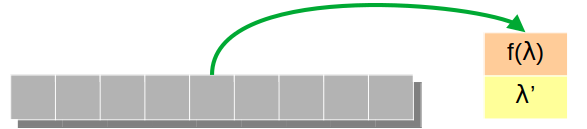
\includegraphics[width=\textwidth]{oracle}
  \label{fig:qafny-oracle-analog}
\end{minipage}
\hfill
\begin{minipage}[t]{0.5\textwidth}
\subcaption{App Function Modeling}
  \begin{mathpar}

    \inferrule[]{\forall j.\;\slen{c_{j1}}=n \\ \Omega;\sigma;\varphi\models \sch{m}{z_j}{\denote{\mu}(c_{j1}).c_{j2}\,\beta_j} \mapsto q}
          {\Omega;\sigma;\varphi\models \eth \;n.\denote{\mu}(\sch{m}{z_j}{c_{j1}.c_{j2}\,\beta_j}) 
              \mapsto q }
  \end{mathpar}
  \label{fig:qafny-mu-model}
\end{minipage}

\begin{minipage}[t]{\textwidth}
\subcaption{Semantic/Proof Rules}
  \begin{mathpar}


    \inferrule[SH-N]{ FV(\emptyset,l)= \kappa \\ \varphi(\kappa)=\ket{c} }{ (\varphi,\ssassign{l}{}{\texttt{H}}) \longrightarrow (\varphi[\kappa\mapsto \shad{2^{\slen{c}}}{\slen{c}}{\alpha(\frac{1}{2^{c[j]}})}],\{\}) }

    \inferrule[PH-N]{FV(\Omega,l)=\kappa \\ \sigma(\kappa)=\tau}
                {\fivepule{\Omega}{\sigma}{g}{P[\eth \;\kappa.\denote{\texttt{H}}(\kappa) / \kappa]}{\ssassign{l}{}{\texttt{H}}}{P}}

  \end{mathpar}
  \label{fig:qafny-oracle-rules}
\end{minipage}
}
\caption{Oracle application and state preparation rules. $\eth$ is an array map operation, where $\eth \;\kappa.\denote{\mu}(\kappa \uplus \kappa')$ means that for every basis state in the state of $\kappa \uplus \kappa'$, we apply $\denote{\mu}$ to $\kappa$ part of session. }
\label{fig:exp-proofsystem-2}
\end{figure*}

\ignore{

\begin{minipage}[t]{0.4\textwidth}
\subcaption{Application Analogy}
  \vspace{1cm}
  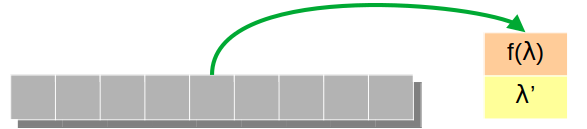
\includegraphics[width=\textwidth]{oracle}
  \label{fig:qafny-oracle-analog}
\end{minipage}
\hfill
\begin{minipage}[t]{0.5\textwidth}
\subcaption{App Function Modeling}
  \begin{mathpar}

}

{\footnotesize
  \begin{mathpar}
\mprset{flushleft}
\inferrule[]{
   \inferrule[]
   { \inferrule[] {
    \fivepule{\Omega}{\sigma_2}{\mmode}{X(\snext{j}) * \{y[0..n]\}\mapsto C(j).1}{ s }{X(\snext{j}) * \{y[0..n]\}\mapsto C'(j).1} }
  { \fivepule{\Omega}{\sigma_2}{\mmode}{X(\snext{j}) * \mathpzc{M}(b,\{y[0..n]\})\mapsto 0.C(j)+1.C(j)}{ s }{X(\snext{j}) * \{y[0..n]\}\mapsto C'(j).1} } }
   {  \Omega,\sigma_1\vdash_{\mmode} \{X(\snext{j}) * \{x[0..\snext{j}],y[0..n]\}\mapsto 0.C(j)+1.C(j)\} \sifq{x[j]}{s}
     \\\\\qquad\qquad \{ X(\snext{j}) * \mathpzc{U}(\neg x[j],\{x[0..\snext{j}],y[0..n]\})\mapsto 0.C(j)
          * \mathpzc{U}(x[j],\{x[0..\snext{j}],y[0..n]\})\mapsto C'(j).1\}
     } } {
\fivepule{\Omega}{\sigma}{\mmode}{X(j) * \{x[0..j],y[0..n]\}\mapsto C(j)}{ \sifq{x[j]}{s} }{X(j\,\sminus\,1) * \{x[0..\snext{j}],y[0..n]\} \mapsto 0.C(j)+1.C'(j)} }
  \end{mathpar}
{\hspace*{-1.5em}
$\begin{array}{l}
X(j)=\shad{2^{n \,\sminus\,  j}}{n \,\sminus\, j}{}
\quad
C(j)=\sch{2^k}{\frac{1}{\sqrt{2^k}}}{\tos{j}^{k}.\tos{a^{\tos{j}^k}\;\%\;N}}
\quad
i.C(j)=\sch{2^{\snext{k}}}{\frac{1}{\sqrt{2^{\snext{k}}}}}{\tos{j}^k.i.\tos{a^{\tos{j}^k}\;\%\;N}}
\\
C'(j).i=\sch{2^{\snext{k}}}{\frac{1}{\sqrt{2^{\snext{k}}}}}{\tos{a^{\tos{j}^k.1}\;\%\;N}\,|\,\tos{j}^k.i}
\qquad
i.C'(j)=\sch{2^{\snext{k}}}{\frac{1}{\sqrt{2^{\snext{k}}}}}{\tos{j}^k.i.\tos{a^{\tos{j}^k.1}\;\%\;N}}
\\
\sigma_1=\{x[0..n\,\sminus\,\snext{j}] \mapsto \thadt, \{x[0..\snext{j}],y[0..n]\} \mapsto \tcht \}
\quad
\sigma=\{x[0..n\,\sminus\,\snext{j}] \mapsto \thadt, y[0..n] \mapsto \tcht \}
\quad
s=\ssassign{y}{}{a^{2^j}y\;\%\; N}
\end{array}$
}
}


\subsection{Additional Proof Rules}\label{appx:proof-rules}

The proof is built from bottom up. We first cut the $\thadt$ type state into two sessions ($x[0..n\,\sminus\,\snext{j}]$ and $x[j]$), join $x[j]$ with session $\{x[0..j],y[0..n]\}$, and double the state elements to be $0.C(j)+1.C(j)$, which is proved by applying the consequence rules. Notice that the type environment is also transitioned from $\sigma$ to $\sigma_1$.
By the same strategy of the $\mathpzc{U}$ rule in \Cref{fig:qafny-mu-model}, we combine the two $\mathpzc{U}$ terms into the final result. 
The second step applies rule \textsc{PIF} to substitute session $\{x[0..\snext{j}],y[0..n]\}$ with the mask construct $\mathpzc{M}(b,\{y[0..n]\})$ in the pre-condition and create two $\mathpzc{U}$ terms in the post-condition. The step on the top applies the modulo multiplication on every element in the masked state $\mapsto C(j).1$ by rule \textsc{PA-CH}.

\begin{figure*}[t]
{\small
  \begin{mathpar}

\hspace*{-1em}
    \inferrule[Frame]{FV(s)\cap FV(R)=\emptyset \\ FV(s)\subseteq \dom{\sigma} \\\\
       \sigma\bot\sigma' \\ \fivepule{\Omega}{\sigma}{g}{P}{s}{Q}}
                {\fivepule{\Omega}{\sigma\cup\sigma'}{g}{P * R}{s}{Q * R}}

    \inferrule[]{\sigma \bot \sigma' \\ \varphi \bot \varphi' 
      \\ \Omega;\sigma; \psi; \varphi \models_g P \\ \Omega;\sigma';\psi; \varphi' \models_g Q}
        {\Omega;\sigma \cup \sigma';\psi; \varphi \cup \varphi'\models_g P * Q }

    \inferrule[SSeq-1]{(\psi,\varphi,s_1) \longrightarrow (\psi',\varphi',s'_1)}{(\psi,\varphi,\sseq{s_1}{s_2})\longrightarrow (\psi',\varphi',\sseq{s'_1}{s_2}) }
\quad
    \inferrule[SSeq-2]{}{(\psi,\varphi,\sseq{\{\}}{s_2})\longrightarrow (\psi,\varphi,s_2) }
\quad
    \inferrule[PSeq]{
          \Omega;\sigma\vdash_g s_1 \triangleright \sigma' \\\\
       \fivepule{\Omega}{\sigma}{g}{P}{s_1}{R} \quad
           \fivepule{\Omega}{\sigma[\uparrow \sigma']}{g}{R}{s_2}{Q}}
                {\fivepule{\Omega}{\sigma}{g}{P}{\sseq{s_1}{s_2}}{Q}}


    \inferrule[PConL]{
       (\Omega,\sigma,P) \Rightarrow (\Omega,\sigma',P') \\ \fivepule{\Omega}{\sigma'}{g}{P'}{s}{Q}}
                {\fivepule{\Omega}{\sigma}{g}{P}{s}{Q}}

    \inferrule[PConR]{\Omega,\sigma\vdash_g s_1 \triangleright \sigma'\\\\
          \fivepule{\Omega}{\sigma'}{g}{P}{s}{Q'} \\(\Omega,\sigma'',Q') \nRightarrow (\Omega,\sigma[\uparrow \sigma'],Q) }
                {\fivepule{\Omega}{\sigma}{g}{P}{s}{Q}}
  \end{mathpar}
}
{\footnotesize
\[
\begin{array}{l}
\\
(\Omega,\sigma,P) \Rightarrow (\Omega,\sigma',P') \triangleq \Omega,\sigma\vdash P \wedge \Omega,\sigma' \vdash P' \wedge \sigma \preceq \sigma' \wedge P \Rightarrow P'
\\[0.2em]
(\Omega,\sigma,Q) \nRightarrow (\Omega,\sigma',Q') \triangleq \Omega,\sigma\vdash Q \wedge \Omega,\sigma' \vdash Q' \wedge \sigma' \preceq \sigma \wedge Q \Rightarrow Q'
\ignore{
\\[0.2em]
\varphi \equiv \varphi' \wedge \varphi \models P \wedge \varphi' \models P' \Rightarrow (P \Leftrightarrow P') 

\\[0.2em]
 q(c_j) = \scha{m}{z_j}{c_{j}}{\beta_j}
\qquad \llbracket \mu \rrbracket c_{j} = z'_j\ket{c'_{j}}
}
\end{array}
\]
}
\caption{Sequence and Consequence Rules}
\label{fig:exp-proofsystem-seq}
\end{figure*}

\subsection{Well-formed Sessions and Predicates}\label{appx:well-formed}

\begin{definition}[Well-formed session domain]\label{def:well-formed-ses}\rm 
  The domain of a environment $\sigma$ (or state $\varphi$) is \emph{well-formed}, written as
  $\Omega \vdash \dom{\sigma}$ (or $\dom{\varphi}$), iff for every session $\kappa\in \dom{\sigma}$ (or $\dom{\varphi}$):
\begin{itemize}
\item $\kappa$ is disjoint unioned, i.e., for every two ranges $x[i..j]$ and $y[i'..j']$, $x[i..j]\cap y[i'..j']=\emptyset$.

\item For every range $x[i..j]\in\kappa$, $\Omega(x)=\qmode{n}$ and $[i,j) \subseteq [0,n)$.
\end{itemize}
\end{definition}

\begin{definition}[Well-formed state predicate]\label{def:well-formed-pred}\rm 
  A predicate $P$ is well-formed, written as $\Omega,\sigma \vdash P$, iff every variable and session appearing in $P$ is defined in $\Omega$ and $\sigma$, respectively; particularly, if $P=\kappa \mapsto q * P'$, $\kappa \in \dom{\sigma}$.
\end{definition}

\begin{figure}{h}
  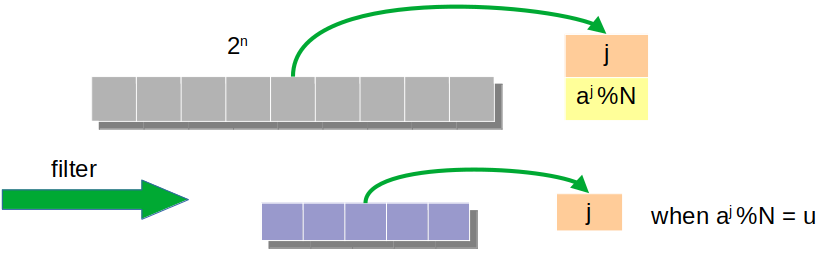
\includegraphics[width=.60\textwidth]{shorsmap}
  \caption{The array analogy of Shor's first half in \Cref{fig:shorqafny}. }
\label{fig:shorsanalog}
\end{figure}




\end{document}
